% Statistiek-samenvatting.tex
% =============================================================================
%           SAMENVATTING STATISTIEK - KU Leuven Industriële Ingenieurs
%           Gebaseerd op: Statistics 12th Edition - McClave & Sincich
% =============================================================================

\documentclass[a4paper,11pt]{article}
% Allow LaTeX to accept files with non-UTF8 bytes (fallback for some editors/encodings)
\UseRawInputEncoding
\usepackage{../../school-macros}

% =============================================================================
%  Fix: colupper=vscodeWhite in codeblock breaks listings catcode setup for
%  special chars (#, _) in Python/SQL code. Use lstnewenvironment directly.
% =============================================================================
\lstnewenvironment{pyblock}[1][]
{%
  \lstset{%
    language=Python,
    basicstyle=\ttfamily\footnotesize\color{vscodeWhite},
    keywordstyle=\color{vscodeBlue}\bfseries,
    stringstyle=\color{vscodeOrange},
    commentstyle=\color{vscodeGreen}\itshape,
    numbers=left, numberstyle=\tiny\color{vscodeGray},
    breaklines=true, tabsize=4,
    showstringspaces=false,
    backgroundcolor=\color{codeBackground},
    xleftmargin=25pt, framexleftmargin=15pt,
    frame=single, framesep=5pt, framerule=0pt,
    fillcolor=\color{codeBackground},
    rulecolor=\color{codeBackground},
    #1%
  }%
}{}

% =============================================================================
%                           DOCUMENT INFO
% =============================================================================
\newcommand{\titel}{Statistiek \& Databeheer -- Statistiek}
\newcommand{\auteur}{KUL Industriële Ingenieurs}
\newcommand{\academiejaar}{Academiejaar 2025-2026}

% =============================================================================
%                              DOCUMENT
% =============================================================================
\begin{document}

\kuleuventitle{\titel}{}{\auteur}{\academiejaar}

\begin{abstract}
Samenvatting van de statistiekcursus (Ch.\ 1--7): beschrijvende statistiek, kansrekening,
discrete en continue kansverdelingen, steekproefverdelingen en betrouwbaarheidsintervallen.\\
Beschikbaar op GitHub: \url{https://github.com/KUL-Industriele-ingenieurs/Samenvattingen-Ku-leuven-Industriele-ingenieurs}
\end{abstract}

\tableofcontents
\newpage

% =============================================================================
%  HOOFDSTUK 1: STATISTISCH DENKEN
% =============================================================================
\section{Ch.\ 1 -- Statistisch denken, Data en Statistiek}

\begin{conceptbox}[Populatie vs.\ Sample]
\textbf{Populatie} \sym{N}{Populatiegrootte}{--} is de volledige verzameling data die we willen bestuderen.\\
\textbf{Sample (steekproef)} \sym{n}{Steekproefgrootte}{--} is een \emph{deelverzameling} van de populatie.\\
\textbf{Experimentele eenheid} is het object waarover we data verzamelen (persoon, ding, transactie\ldots).
\end{conceptbox}

\subsection{Soorten statistiek}
\begin{itemize}
  \item \textbf{Beschrijvende statistiek} -- patronen zoeken en presenteren in bestaande data (een gegeven dataset beschrijven).
  \item \textbf{Verklarende/voorspellende statistiek} -- een sample gebruiken om uitspraken (schattingen, beslissingen, voorspellingen) te doen over de populatie.
\end{itemize}

\subsection{Soorten data}

\begin{conceptbox}[Kwantitatief vs.\ Kwalitatief]
\begin{itemize}
  \item \textbf{Kwantitatief (numeriek)} -- meetbare waarden op een numerieke schaal, bv.\ $47\,\text{ms}$, $13\,\text{ms}$.
  \item \textbf{Kwalitatief (categorisch)} -- categorieën zonder natuurlijke numerieke schaal, bv.\ Porsche / Audi / BMW of Ja / Nee.
\end{itemize}
\end{conceptbox}

\subsection{Soorten steekproeven \& dataverzameling}
\begin{itemize}
  \item \textbf{Ontworpen experiment} -- de onderzoeker heeft volledige controle over de eigenschappen van de experimentele eenheden (bv.\ controlegroep vs.\ behandelingsgroep).
  \item \textbf{Waarnemend (observationeel) onderzoek} -- eenheden worden geobserveerd in hun natuurlijke omgeving, zonder controle.
  \item \textbf{Representatieve steekproef} -- weerspiegelt de populatie correct.
  \item \textbf{Willekeurige (aselecte) steekproef} -- elk element heeft gelijke kans om gekozen te worden.
\end{itemize}

\begin{conceptbox}[Typische fouten bij dataverzameling]
\begin{itemize}
  \item \textbf{Selectiebias} -- een deel van de populatie wordt systematisch uitgesloten.
  \item \textbf{Non-response bias} -- geselecteerde eenheden zijn niet bereikbaar (bv.\ politieke enquêtes).
  \item \textbf{Meetfout} -- onnauwkeurigheden in de geregistreerde data (bv.\ dubbelzinnige vragen).
\end{itemize}
\end{conceptbox}

\newpage
% =============================================================================
%  HOOFDSTUK 2: BESCHRIJVEN VAN DATASETS
% =============================================================================
\section{Ch.\ 2 -- Methodes voor het beschrijven van datasets}

\subsection{Kwalitatieve data}
Kwalitatieve data wordt ingedeeld in \textbf{klassen}:
\begin{itemize}
  \item \textbf{Class frequency} -- hoe vaak een observatie in een klasse voorkomt.
  \item \textbf{Relatieve class frequency} -- class frequency gedeeld door $n$; kan in \% uitgedrukt worden.
\end{itemize}
Grafieken: pie chart, bar graph, Pareto-diagram.

\subsection{Kwantitatieve data -- Centrummaten}

\begin{figure}[h!]
  \centering
  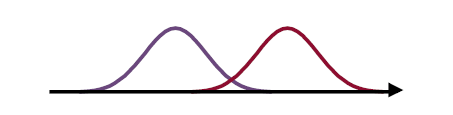
\includegraphics[width=0.55\textwidth]{assets/central tendency.png}
  \caption{Centrale tendentie (centrum) en spreiding van een dataset.}
\end{figure}

\frm{Steekproefgemiddelde}{\bar{x} = \frac{\displaystyle\sum_{i=1}^{n} x_i}{n}}{%
  $\bar{x}$ = steekproefgemiddelde, $x_i$ = waarnemingen, $n$ = steekproefgrootte.
  Wordt gebruikt om het populatiegemiddelde \sym{\mu}{Populatiegemiddelde}{--} te schatten.}

\begin{conceptbox}[Mediaan]
De \textbf{mediaan} $M$ is de middelste waarde na sortering in oplopende volgorde.
\begin{itemize}
  \item Als $n$ oneven: mediaan = middelste getal.
  \item Als $n$ even: mediaan = gemiddelde van de twee middelste getallen.
\end{itemize}
De mediaan is \emph{minder gevoelig voor uitschieters} dan het gemiddelde.
Het oppervlak links van de mediaan in het histogram = oppervlak rechts.
\end{conceptbox}

\begin{conceptbox}[Modus]
De \textbf{modus} is de waarde die het \emph{vaakst voorkomt} in de dataset.
\end{conceptbox}

\begin{figure}[h!]
  \centering
  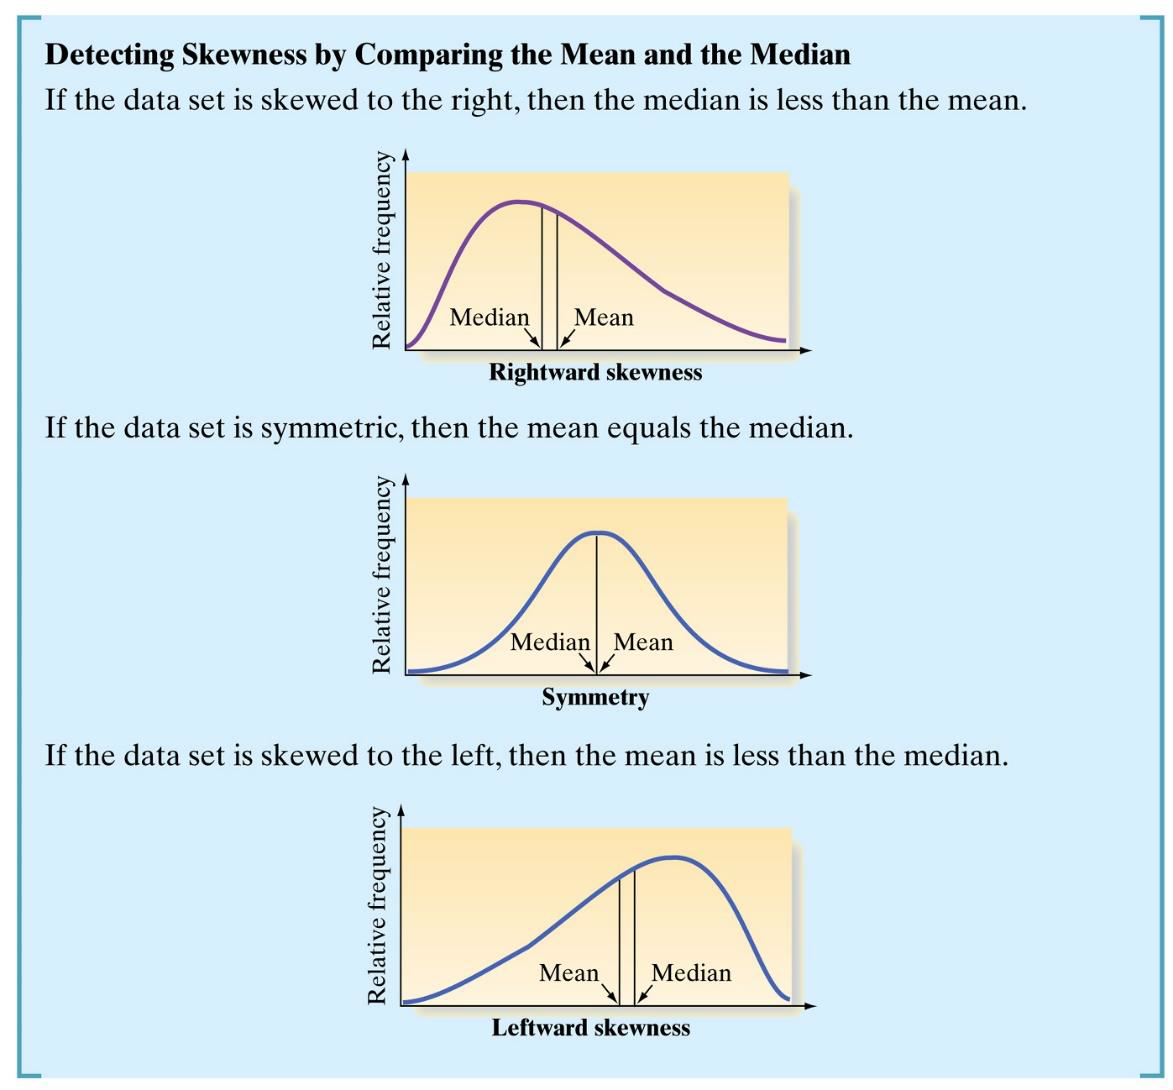
\includegraphics[width=0.65\textwidth]{assets/verschilmediaangemiddelde.png}
  \caption{Verschil tussen mediaan en gemiddelde bij scheve data (skewed).}
\end{figure}

\begin{conceptbox}[Scheefheid (Skewness)]
Bij een \textbf{scheve verdeling} heeft één staart meer extreme waarden dan de andere:
\begin{itemize}
  \item \textbf{Rechts scheef (positief)}~-- lange staart naar rechts; gemiddelde $>$ mediaan.
  \item \textbf{Links scheef (negatief)}~-- lange staart naar links; gemiddelde $<$ mediaan.
\end{itemize}
Bij een symmetrische, klokvormige verdeling vallen gemiddelde, mediaan en modus samen.
\end{conceptbox}

\subsection{Kwantitatieve data -- Spreidingsmaten}

\frm{Bereik (range)}{R = x_{\max} - x_{\min}}{Eenvoudigste spreidingsmaat; gevoelig voor uitschieters.}

\frm{Sample variantie}{s^2 = \frac{\displaystyle\sum_{i=1}^{n}(x_i - \bar{x})^2}{n-1}}{%
  $s^2$ = steekproefvariantie \sym{s^2}{Steekproefvariantie}{--}.
  Deling door $n-1$ (niet $n$) voorkomt onderschatting van de populatievariantie.}

\frm{Populatievariantie}{\sigma^2 = \frac{\displaystyle\sum_{i=1}^{N}(x_i - \mu)^2}{N}}{%
  $\sigma^2$ = populatievariantie \sym{\sigma^2}{Populatievariantie}{--}, $N$ = populatiegrootte.}

\frm{Standaardafwijking}{s = \sqrt{s^2} \quad \text{(sample)} \qquad \sigma = \sqrt{\sigma^2} \quad \text{(populatie)}}{%
  \sym{s}{Steekproef standaardafwijking}{--} \quad \sym{\sigma}{Populatie standaardafwijking}{--}}

\begin{figure}[h!]
  \centering
  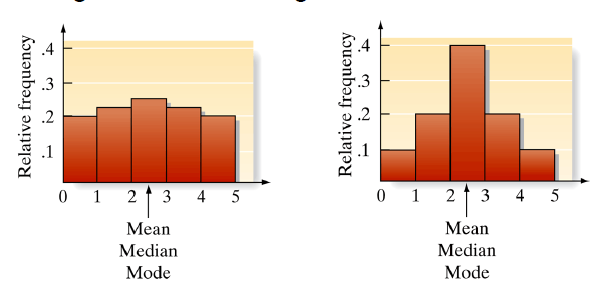
\includegraphics[width=0.6\textwidth]{assets/spreiding.png}
  \caption{Visuele weergave van spreiding/variabiliteit van een dataset.}
\end{figure}


\begin{pyblock}
import numpy as np

data = [4, 7, 13, 2, 1, 9, 6]
print(np.mean(data))            # gemiddelde
print(np.median(data))          # mediaan
print(np.std(data, ddof=1))     # steekproef std s
print(np.var(data, ddof=1))     # steekproef variantie s^2
Q1, Q3 = np.percentile(data, [25, 75])
print(f"IQR = {Q3 - Q1}")
# Z-score van een waarde:
z = (9 - np.mean(data)) / np.std(data, ddof=1)
\end{pyblock}
\subsection{Betekenis van de standaardafwijking}

\begin{theorieblok}[Empirische Regel -- geldig voor klokvormige (symmetrische) verdelingen]
\begin{itemize}
  \item \textbf{68\%} van alle metingen ligt tussen $\bar{x} - s$ en $\bar{x} + s$ \quad (of $\mu \pm \sigma$).
  \item \textbf{95\%} van alle metingen ligt tussen $\bar{x} - 2s$ en $\bar{x} + 2s$ \quad (of $\mu \pm 2\sigma$).
  \item \textbf{99{,}7\%} van alle metingen ligt tussen $\bar{x} - 3s$ en $\bar{x} + 3s$ \quad (of $\mu \pm 3\sigma$).
\end{itemize}
\end{theorieblok}

\begin{figure}[h!]
  \centering
  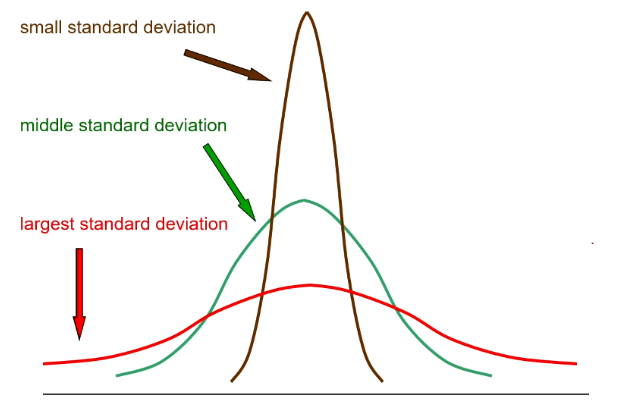
\includegraphics[width=0.65\textwidth]{assets/Standaardafwijking effect.png}
  \caption{Effect van de standaardafwijking op de verdeling.}
\end{figure}

\subsection{Percentielenpositie en Z-score}

\begin{conceptbox}[Percentielen en Kwartielen]
Het \textbf{$p$-de percentiel} is de waarde waarbij $p\%$ van de data hieronder valt en $(100-p)\%$ hierboven.
\begin{itemize}
  \item \sym{Q_1}{25\%-percentiel (onderste kwartiel)}{--} -- 25\% van alle waarnemingen ligt hieronder.
  \item $Q_2$ = mediaan (50\%-percentiel).
  \item \sym{Q_3}{75\%-percentiel (bovenste kwartiel)}{--} -- 75\% van alle waarnemingen ligt hieronder.
  \item \sym{\text{IQR}}{Interkwartielafstand}{--} $= Q_3 - Q_1$ \quad (bevat 50\% van de data).
\end{itemize}
\end{conceptbox}

\frm{Z-score (sample)}{z = \frac{x - \bar{x}}{s}}{Gestandaardiseerde afstand van een waarde tot het gemiddelde.}

\frm{Z-score (populatie)}{z = \frac{x - \mu}{\sigma}}{}

\begin{conceptbox}[Interpretatie Z-score]
\begin{itemize}
  \item 68\% van alle metingen: $-1 < z < 1$
  \item 95\% van alle metingen: $-2 < z < 2$
  \item 99{,}7\% van alle metingen: $-3 < z < 3$
  \item Mogelijke uitschieter: $|z| > 2$
  \item Uitschieter: $|z| > 3$ (heel verdacht)
\end{itemize}
\end{conceptbox}

\subsection{Boxplot en uitschieters detecteren}

\begin{figure}[h!]
  \centering
  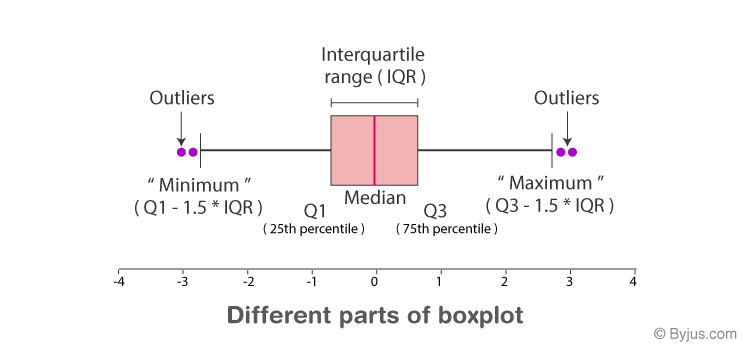
\includegraphics[width=0.72\textwidth]{assets/boxplot.png}
  \caption{Boxplot -- handige tool om uitschieters te detecteren.}
\end{figure}

\begin{conceptbox}[Uitschieters via IQR -- boxplot]
\begin{itemize}
  \item \textbf{Verdachte uitschieter} als kleiner dan $Q_1 - 1{,}5 \cdot \text{IQR}$ of groter dan $Q_3 + 1{,}5 \cdot \text{IQR}$.
  \item \textbf{Extreem verdachte uitschieter} als verder dan $Q_1 - 3 \cdot \text{IQR}$ of $Q_3 + 3 \cdot \text{IQR}$ (equivalent met $|z| > 3$).
\end{itemize}
Oorzaken van uitschieters: (1) meetfout, (2) waarde afkomstig van andere populatie, (3) correcte maar zeldzame waarde.
\end{conceptbox}

\newpage
% =============================================================================
%  HOOFDSTUK 3: PROBABILITEIT (KANSREKENING)
% =============================================================================
\section{Ch.\ 3 -- Probabiliteit (Kansrekening)}

\subsection{Basisconcepten}

\begin{conceptbox}[Terminologie]
\begin{itemize}
  \item \textbf{Experiment} -- een handeling die een uitkomst geeft die niet zeker bepaald is (bv.\ dobbelsteen gooien, munt opgooien).
  \item \textbf{Sample point} -- de meest basale mogelijke uitkomst van een experiment (bv.\ ``kop'' of ``munt'').
  Bij 2 munten gooien heb je 4 sample points: KK, KM, MK, MM.
  \item \textbf{Sample space $S$} -- de verzameling van \emph{alle} mogelijke sample points, weergegeven via boomdiagram of Venn-diagram.
  \item \textbf{Event} -- een specifieke deelverzameling van sample points. Bv.\ ``even getal'' bij dobbelsteen = $\{2, 4, 6\}$.
\end{itemize}
\end{conceptbox}

\begin{figure}[h!]
  \centering
  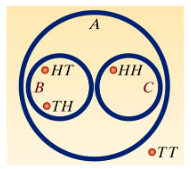
\includegraphics[width=0.6\textwidth]{assets/munten met meerdere events.png}
  \caption{Sample space bij het gooien van meerdere munten.}
\end{figure}

\begin{theorieblok}[Kansregels voor sample points]
Als $p_i$ de kans is voor sample point $i$:
\begin{enumerate}
  \item $0 \leq p_i \leq 1$
  \item $\displaystyle\sum_i p_i = 1$ \quad (som van alle kansen in de sample space is 1)
\end{enumerate}
\textbf{De kans op een event} = som van de kansen van de bijhorende sample points.\\
Bv.\ bij dobbelsteen: $P(\text{even}) = P(2) + P(4) + P(6) = \tfrac{1}{6}+\tfrac{1}{6}+\tfrac{1}{6} = \tfrac{1}{2}$.
\end{theorieblok}

\begin{figure}[h!]
  \centering
  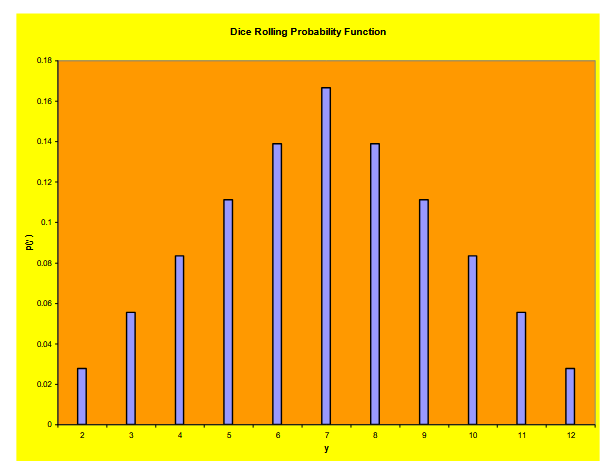
\includegraphics[width=0.6\textwidth]{assets/kansverdeling-2dobbelstenen.png}
  \caption{Kansverdeling bij het gooien van 2 dobbelstenen.}
\end{figure}

\subsection{Vereniging, Doorsnede en Complement}

\begin{figure}[h!]
  \centering
  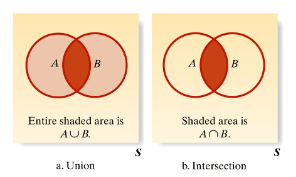
\includegraphics[width=0.55\textwidth]{assets/union and intersection.png}
  \caption{Unie $A \cup B$ en Doorsnede $A \cap B$ via Venn-diagram.}
\end{figure}

\begin{conceptbox}[Union, Intersection \& Complement]
Stel: $A$ = even getallen $= \{2,4,6\}$ en $B$ = 3 of kleiner $= \{1,2,3\}$ bij een dobbelsteen.
\begin{itemize}
  \item \textbf{Unie} $A \cup B$ -- alles in A \emph{of} B: $\{1,2,3,4,6\}$.
  \item \textbf{Doorsnede} $A \cap B$ -- alles in A \emph{en} B: $\{2\}$.
  \item \textbf{Complement} $A^c = S - A$ -- alle sample points \emph{niet} in A: $\{1,3,5\}$.
\end{itemize}
\end{conceptbox}

\frm{Somregel (Additive Rule)}{P(A \cup B) = P(A) + P(B) - P(A \cap B)}{%
  Aftrekken van de doorsnede om dubbeltelling te vermijden.}

\frm{Complementregel}{P(A) + P(A^c) = 1}{}

\begin{conceptbox}[Mutueel exclusief (disjunct)]
A en B zijn \textbf{mutueel exclusief} als ze geen gemeenschappelijke sample points hebben:
\[P(A \cap B) = 0 \;\Rightarrow\; P(A \cup B) = P(A) + P(B)\]
Complementaire events zijn \emph{altijd} mutueel exclusief, maar het omgekeerde geldt niet altijd.
Mutueel exclusieve events zijn \emph{afhankelijk} van elkaar.
\end{conceptbox}

\begin{figure}[h!]
  \centering
  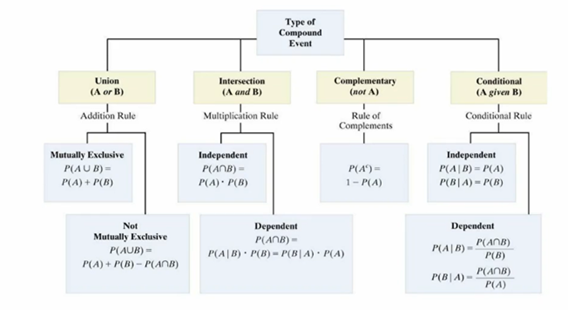
\includegraphics[width=0.65\textwidth]{assets/samenvatting kansrekenen.png}
  \caption{Samenvatting van de kansrekenregels.}
\end{figure}

\subsection{Voorwaardelijke kans}

\frm{Voorwaardelijke kans}{P(A \mid B) = \frac{P(A \cap B)}{P(B)}}{%
  $P(A \mid B)$ = kans dat A optreedt, \emph{wetende} dat B al is gebeurd.\\
  Bv.\ bij dobbelsteen, $B$ = getal is 3 of kleiner:
  $P(2 \mid B) = \dfrac{P(\{2\})}{P(\{1,2,3\})} = \dfrac{1/6}{3/6} = \dfrac{1}{3}$ (normaal was $\tfrac{1}{6}$).}

\frm{Productregel (Multiplicative Rule)}{P(A \cap B) = P(B) \cdot P(A \mid B) = P(A) \cdot P(B \mid A)}{}

\begin{conceptbox}[Onafhankelijke events]
A en B zijn \textbf{onafhankelijk} als het optreden van B \emph{geen invloed} heeft op de kans van A:
\[P(A \mid B) = P(A) \quad\Leftrightarrow\quad P(B \mid A) = P(B) \quad\Leftrightarrow\quad P(A \cap B) = P(A) \cdot P(B)\]
\textbf{Opmerking:} dit werkt in beide richtingen -- je kan $P(A \cap B) = P(A) \cdot P(B)$ gebruiken om onafhankelijkheid te \emph{bewijzen of te weerleggen}. Onafhankelijkheid kan \emph{niet} worden afgelezen uit een Venn-diagram.
\end{conceptbox}

\subsection{Combinatieleer}

\frm{Multiplicatieregel}{n_1 \cdot n_2 \cdot n_3 \cdots n_k}{%
  Bij $k$ sets met resp.\ $n_1, n_2, \ldots, n_k$ elementen: zo veel verschillende steekproeven (neem 1 element uit elke set).}

\frm{Permutatie}{P_n^N = N(N-1)(N-2)\cdots(N-n+1) = \frac{N!}{(N-n)!}}{%
  Aantal manieren om $n$ elementen te \emph{rangschikken} (volgorde telt!) uit een groep van $N$.
  De set wordt na elk trekken steeds kleiner.}

\frm{Partitie}{\frac{N!}{n_1!\, n_2!\, \cdots\, n_k!}}{%
  Verdeel groep van $N$ in $k$ groepen waarbij $n_1 + n_2 + \cdots + n_k = N$.
  Aantal verschillende indelingen.}

\frm{Combinatie}{\binom{N}{n} = \frac{N!}{n!\,(N-n)!}}{%
  Aantal manieren om $n$ elementen te kiezen uit $N$ \emph{zonder} teruglegging (volgorde telt \emph{niet}).
  Speciaal geval van partitie met $k=2$.}

\subsection{Regel van Bayes}

\begin{theorieblok}[Regel van Bayes]
Gegeven oorzaken $B_1, B_2, \ldots, B_k$ die \emph{mutueel exclusief} zijn en waarvan de som van de kansen 1 is.
Gegeven gevolg $A$:
\[
  P(B_i \mid A) = \frac{P(B_i)\cdot P(A \mid B_i)}{\displaystyle\sum_{j=1}^{k} P(B_j)\cdot P(A \mid B_j)}
\]
\textbf{Vraag:} wat is de kans op oorzaak $B_i$, gegeven dat gevolg $A$ heeft plaatsgevonden?\\
\textbf{Voorwaarden:} (1) oorzaken kunnen niet tegelijkertijd optreden, (2) som van kansen van oorzaken = 1.
\end{theorieblok}

\begin{figure}[h!]
  \centering
  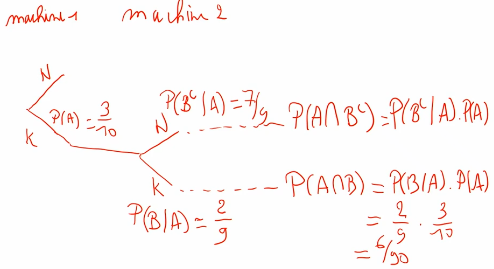
\includegraphics[width=0.62\textwidth]{assets/boomdiagram.png}
  \caption{Boomdiagram -- handig hulpmiddel bij kansberekeningen met meerdere stappen.}
\end{figure}

\newpage
% =============================================================================
%  HOOFDSTUK 4: DISCRETE RANDOM VARIABLES
% =============================================================================
\section{Ch.\ 4 -- Discrete Random Variables (Discrete Kansverdeling)}

\begin{conceptbox}[Stochastische variabele (random variable)]
Een \textbf{willekeurige (stochastische) variabele} is een variabele die een \emph{numerieke} waarde toegewezen krijgt op basis van een kansexperiment, zodat je ermee kan rekenen.

Bv.\ bij 2 munten gooien ken je aan elke uitkomst het aantal keer kop $x$ toe:
\begin{center}
KK $\to x=2$, \quad KM $\to x=1$, \quad MK $\to x=1$, \quad MM $\to x=0$
\end{center}

\textbf{Soorten:}
\begin{itemize}
  \item \textbf{Discrete stochastische variabele (tellen)} -- telbare waarden (vaak geheel).
  Bv.\ aantal keer kop, aantal defecten.
  \item \textbf{Continue stochastische variabele (meten)} -- kan elke mogelijke reële waarde aannemen.
  Bv.\ temperatuur, tijd, gewicht.
\end{itemize}
\end{conceptbox}

\subsection{Probability Mass Function (PMF)}

\begin{theorieblok}[Kansverdelingsfunctie voor discrete variabele]
Een \textbf{Probability Mass Function (PMF)} is een grafiek, tabel of formule die de kans $p(x)$ geeft op elke mogelijke uitkomst $x$ van de stochastische variabele.

\textbf{Twee voorwaarden:}
\begin{enumerate}
  \item $p(x) \geq 0$ voor alle waarden van $x$
  \item $\displaystyle\sum_{\text{alle } x} p(x) = 1$
\end{enumerate}
\end{theorieblok}

\frm{Cumulatieve verdelingsfunctie (CDF)}{F(x_0) = \sum_{x \leq x_0} p(x)}{%
  Telt de kansen \emph{oplopend} op van de kleinste waarde tot en met $x_0$.
  Bij de maximale waarde: $F(x_{\max}) = 1$.}


\begin{pyblock}
from scipy import stats as sts

# Voorbeeld: binomiaal (zie sectie 4.4)
rv = sts.binom(n=10, p=0.3)
print(rv.pmf(3))    # P(X = 3) -- puntskans
print(rv.cdf(3))    # P(X <= 3) -- cumulatief
print(rv.sf(3))     # P(X > 3) = 1 - cdf(3)
\end{pyblock}
\subsection{Verwachtingswaarde en Spreiding}

\frm{Verwachtingswaarde (gemiddelde)}{\mu = E(x) = \sum x \cdot p(x)}{%
  \sym{\mu}{Verwachtingswaarde van discrete variabele}{--}
  Gewogen gemiddelde van alle mogelijke uitkomsten.}

\frm{Variantie}{\sigma^2 = E\!\left[(x-\mu)^2\right] = \sum (x-\mu)^2 \cdot p(x) = \sum x^2 \cdot p(x) - \mu^2}{}

\frm{Standaardafwijking}{\sigma = \sqrt{\sigma^2}}{}

\subsection{Chebyshev vs.\ Empirische Regel}

\begin{figure}[h!]
  \centering
  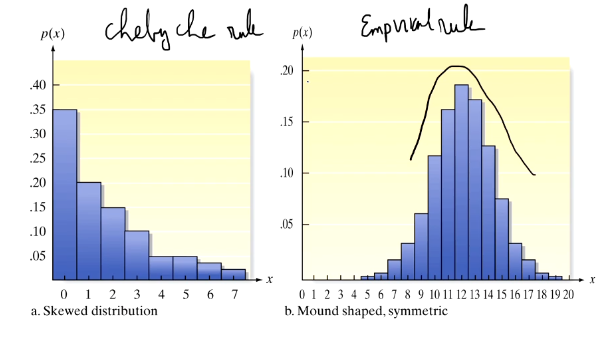
\includegraphics[width=0.68\textwidth]{assets/cheby VS emperical.png}
  \caption{Vergelijking Chebyshev vs.\ Empirische Regel -- geldigheid en grenzen.}
\end{figure}

\begin{theorieblok}[Regel van Chebyshev -- altijd geldig]
\begin{itemize}
  \item Minstens $\tfrac{3}{4}$ (75\%) van de waarnemingen valt tussen $\mu \pm 2\sigma$.
  \item Minstens $\tfrac{8}{9} \approx 89\%$ van de waarnemingen valt tussen $\mu \pm 3\sigma$.
  \item Geen garantie voor $\mu \pm \sigma$.
\end{itemize}
\end{theorieblok}

\begin{examenbox}
De empirische regel geldt \emph{alleen} bij symmetrische/klokvormige verdelingen.
De regel van Chebyshev geldt \emph{altijd} (ook bij scheve verdelingen).
\end{examenbox}

\subsection{De Binomiale Verdeling}

\begin{conceptbox}[Wanneer gebruik je de binomiale verdeling?]
\begin{itemize}
  \item Precies 2 mogelijke uitkomsten per experiment: Succes (S) of Faal (F).
  \item $n$ \emph{onafhankelijke} experimenten.
  \item Kans op succes $p$ blijft constant; kans op faal $q = 1 - p$.
  \item $x$ = totaal aantal successen in $n$ experimenten; $x = 0, 1, 2, \ldots, n$.
\end{itemize}
\end{conceptbox}

\frm{Binomiale PMF}{p(x) = \binom{n}{x} p^x q^{n-x}}{%
  $\binom{n}{x} = \dfrac{n!}{x!\,(n-x)!}$ \quad (aantal manieren om $x$ successen te kiezen uit $n$ pogingen)}

\frm{Gemiddelde (binomiaal)}{\mu = np}{}

\frm{Variantie (binomiaal)}{\sigma^2 = npq \qquad \sigma = \sqrt{npq}}{}

\begin{figure}[h!]
  \centering
  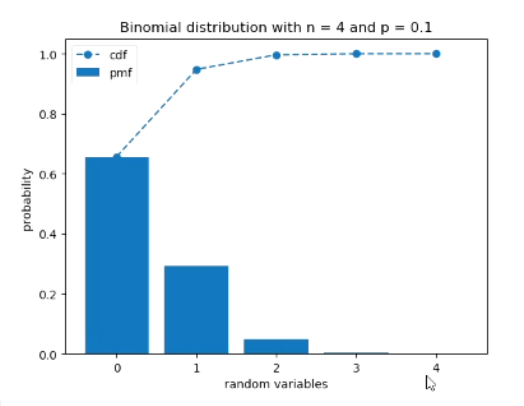
\includegraphics[width=0.65\textwidth]{assets/binomiale-verdeling.png}
  \caption{Voorbeeld van een binomiale kansverdeling.}
\end{figure}


\begin{pyblock}
from scipy import stats as sts
import numpy as np

rv = sts.binom(n=10, p=0.3)       # n pogingen, p slagingskans

# Kansen:
print(rv.pmf(3))                   # P(X = 3)
print(rv.cdf(3))                   # P(X <= 3)
print(1 - rv.cdf(3))               # P(X > 3)
print(rv.cdf(5) - rv.cdf(2))       # P(3 <= X <= 5)

# Statistieken:
print(rv.mean(), rv.std())         # mu = np, sigma = sqrt(npq)

# Inverse (percentielen):
print(rv.ppf(0.95))                # kleinste x met P(X<=x) >= 0.95
\end{pyblock}
\subsection{De Poisson-verdeling}

\begin{conceptbox}[Wanneer gebruik je de Poisson-verdeling?]
De Poisson-verdeling telt het \emph{aantal keren} dat een event optreedt in een gegeven tijdseenheid, oppervlakte of volume:
\begin{itemize}
  \item De kans dat een event optreedt is dezelfde voor alle eenheden.
  \item Events in verschillende eenheden zijn \emph{onafhankelijk}.
  \item Het gemiddeld aantal events per eenheid is $\lambda$ \sym{\lambda}{Gemiddeld aantal events per eenheid (Poisson)}{--}.
\end{itemize}
\end{conceptbox}

\frm{Poisson PMF}{p(x) = \frac{\lambda^x e^{-\lambda}}{x!} \qquad x = 0, 1, 2, \ldots}{%
  $\lambda$ = gemiddeld aantal events per eenheid, $e \approx 2{,}718$.}

\frm{Gemiddelde \& variantie (Poisson)}{\mu = \lambda \qquad \sigma^2 = \lambda \qquad \sigma = \sqrt{\lambda}}{}

\newpage
% =============================================================================
%  HOOFDSTUK 5: CONTINUE RANDOM VARIABLES
% =============================================================================

\begin{pyblock}
from scipy import stats as sts

rv = sts.poisson(mu=2.5)           # lambda = 2.5

print(rv.pmf(3))                   # P(X = 3)
print(rv.cdf(3))                   # P(X <= 3)
print(rv.sf(3))                    # P(X > 3)
print(rv.mean(), rv.std())         # mu=lambda, sigma=sqrt(lambda)
\end{pyblock}
\section{Ch.\ 5 -- Continue Random Variables (Continue Kansverdeling)}

% Introductie
In het vorige hoofdstuk werkten we met \emph{discrete} stochastische variabelen -- variabelen die je kan \emph{tellen} (0, 1, 2, \ldots). Nu stappen we over naar \emph{continue} variabelen: dingen die je \emph{meet}, zoals tijd, temperatuur of gewicht. Deze kunnen oneindig veel waarden aannemen en we kunnen ze niet meer als losse sprongen tekenen.

\subsection{5.1 -- PDF vs.\ PMF: het grote verschil}

\begin{figure}[h!]
  \centering
  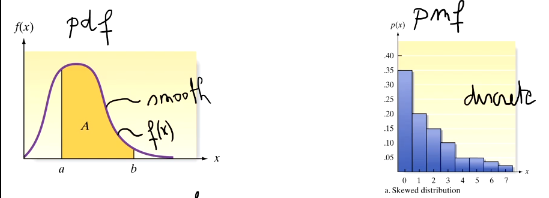
\includegraphics[width=0.70\textwidth]{assets/pdf vs pmf.png}
  \caption{Links de PMF (discrete spikes), rechts de PDF (vloeiende curve). De kans zit in de \emph{oppervlakte}, niet in de hoogte.}
\end{figure}

\begin{conceptbox}[Discreet vs.\ Continu -- het kernverschil]
Bij een \textbf{discrete} variabele (PMF) heeft elke waarde een hoogte = kans, en je telt gewoon alle kansen bij elkaar op.

Bij een \textbf{continue} variabele (PDF) heeft een enkel punt \emph{geen} kans: $P(x = a) = 0$. Dat klinkt raar, maar denk eraan: wat is de kans dat iemand exact 1{,}8000000\ldots m groot is? Nul. Wél zinvol is de kans dat iemand tussen 1{,}79 m en 1{,}81 m valt -- dat is een \emph{oppervlakte} onder de curve.

\textbf{Gevolg:} $P(a < x < b) = P(a \leq x \leq b)$ -- het maakt niet uit of de grenzen inclusief of exclusief zijn bij continue variabelen.
\end{conceptbox}

\frm{PDF -- Kans over een interval}{P(a < x < b) = \int_a^b f(x)\,dx}{%
  \sym{f(x)}{Probability Density Function (kansdichtheidsfunctie)}{--}
  De volledige oppervlakte onder de curve is altijd 1: $\displaystyle\int_{-\infty}^{+\infty} f(x)\,dx = 1$.}

\begin{figure}[h!]
  \centering
  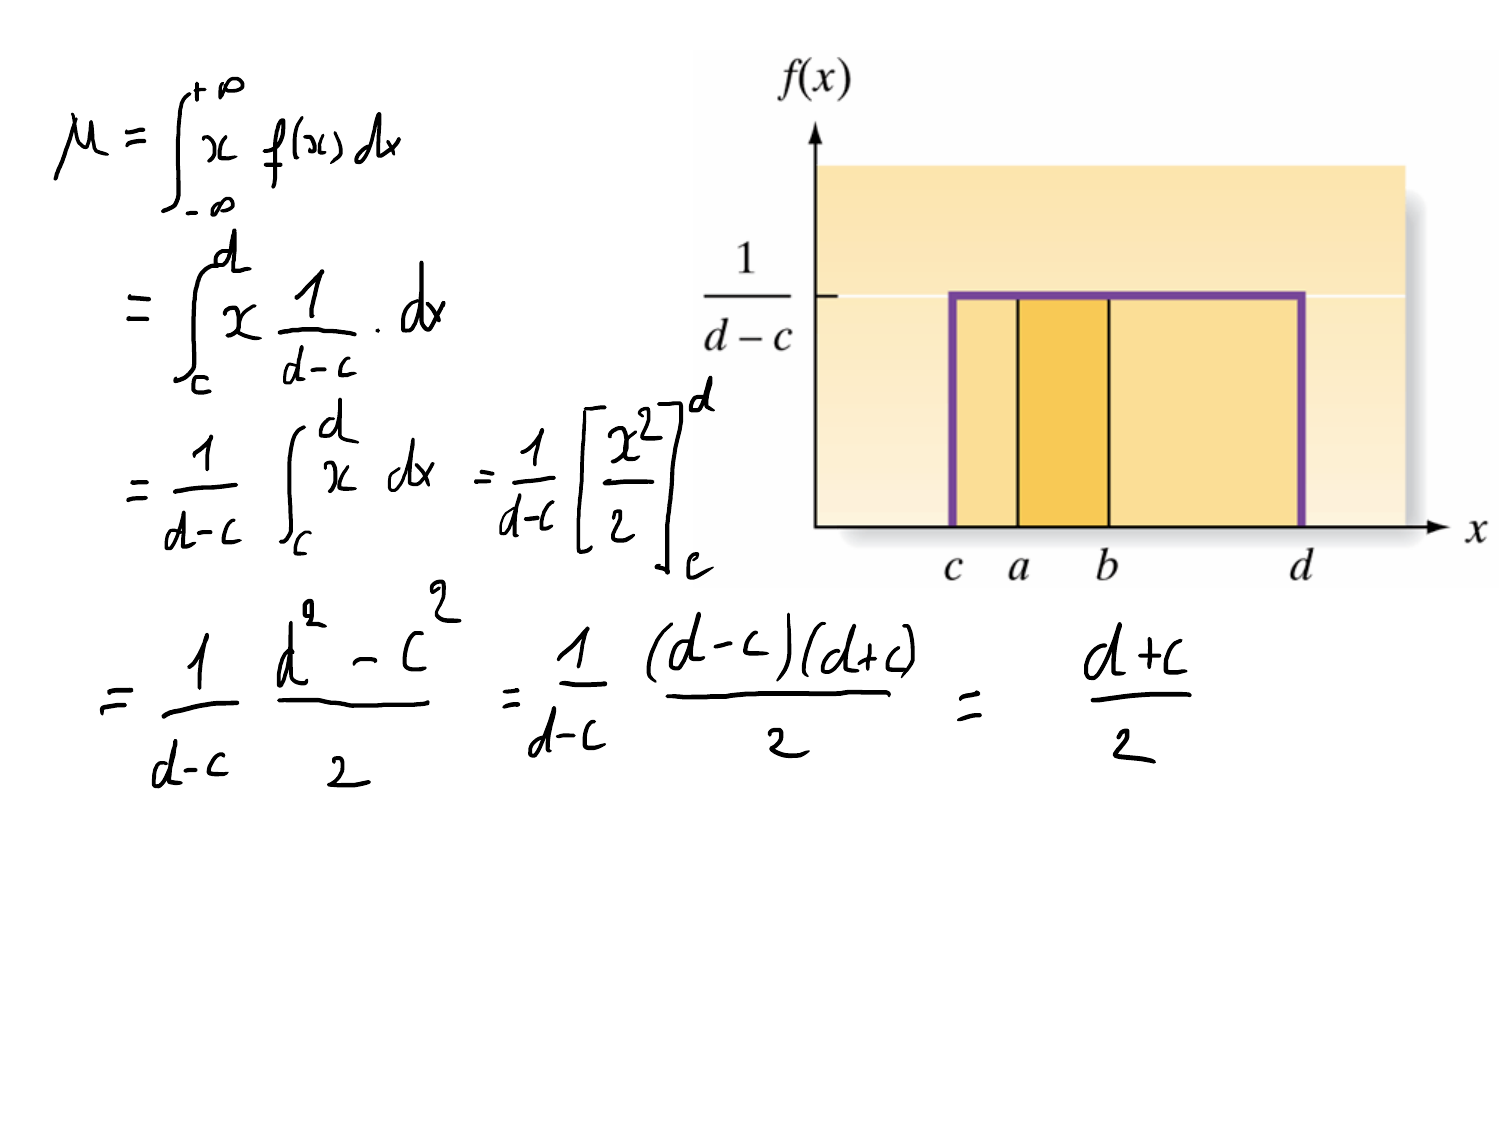
\includegraphics[width=0.72\textwidth]{assets/ch5-mean-variance-continue.png}
  \caption{Gemiddelde en variantie voor een continue kansverdeling $f(x)$.}
\end{figure}

\frm{Gemiddelde (continue variabele)}{\mu = E(x) = \int_{-\infty}^{+\infty} x\, f(x)\,dx}{%
  Hetzelfde idee als bij discrete variabelen ($\mu = \sum x \cdot p(x)$), maar de som wordt een integraal.}

\frm{Variantie (continue variabele)}{\sigma^2 = E\!\left[(x-\mu)^2\right] = \int_{-\infty}^{+\infty}(x-\mu)^2\, f(x)\,dx = E(x^2) - \mu^2}{}

\subsection{5.2 -- De Uniforme verdeling}



\begin{conceptbox}[Intuïtie: uniforme verdeling]
Stel je voor dat een bus elke 10 minuten passeert en je aankomt op een willekeurig tijdstip. De wachttijd $x$ is uniform verdeeld tussen 0 en 10 minuten -- elke wachttijd tussen 0 en 10 min is even waarschijnlijk. De PDF is een plat blok met hoogte $\frac{1}{d-c}$ zodat het totale oppervlak precies 1 is.
\end{conceptbox}

\frm{Uniforme PDF}{f(x) = \frac{1}{d-c} \qquad c \leq x \leq d \quad \text{(en } f(x)=0 \text{ buiten dit interval)}}{%
  $c$ = minimum, $d$ = maximum.}

\frm{Kans over deelinterval}{P(a < x < b) = \frac{b-a}{d-c} \qquad c \leq a < b \leq d}{%
  Dit is gewoon de breedte van het gewenste stuk gedeeld door de totale breedte -- logisch!}

\frm{Gemiddelde en standaardafwijking (uniform)}{\mu = \frac{c+d}{2} \qquad \sigma = \frac{d-c}{\sqrt{12}}}{%
  Het gemiddelde ligt precies in het midden. De standaardafwijking is iets kleiner dan de helft van de breedte.}


\begin{pyblock}
from scipy import stats as sts

c, d = 2, 8                        # minimum, maximum
rv = sts.uniform(loc=c, scale=d-c) # let op: scale = d - c !

print(rv.pdf(5))                   # f(5) = 1/(d-c)
print(rv.cdf(5))                   # P(X <= 5)
print(rv.mean(), rv.std())         # mu=(c+d)/2, sigma=(d-c)/sqrt(12)
# Kans op interval [a, b]:
a, b = 3, 6
print(rv.cdf(b) - rv.cdf(a))      # P(a < X < b)
\end{pyblock}
\subsection{5.3 -- De Normale verdeling}

De \textbf{normale verdeling} is veruit de belangrijkste continue verdeling in de statistiek. Ze duikt op bij bijna alles: lengte van mensen, meetfouten, testresultaten, \ldots. Dit is geen toeval -- de Centrale Limietstelling (Ch.\ 6) legt uit \emph{waarom} dat zo is.

\begin{figure}[h!]
  \centering
  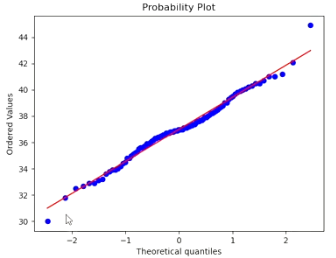
\includegraphics[width=0.65\textwidth]{assets/normaal verdeling plot.png}
  \caption{De klassieke klokvorm van de normale verdeling, symmetrisch rond $\mu$.}
\end{figure}

\frm{Normale PDF}{f(x) = \frac{1}{\sigma\sqrt{2\pi}}\, \exp\!\left[-\frac{1}{2}\left(\frac{x-\mu}{\sigma}\right)^2\right]}{%
  $\mu$ = gemiddelde (bepaalt de ligging), $\sigma$ = standaardafwijking (bepaalt de breedte).\\
  De curve is volledig bepaald door deze twee parameters. Notatie: $x \sim \mathcal{N}(\mu, \sigma^2)$.}

\begin{figure}[h!]
  \centering
  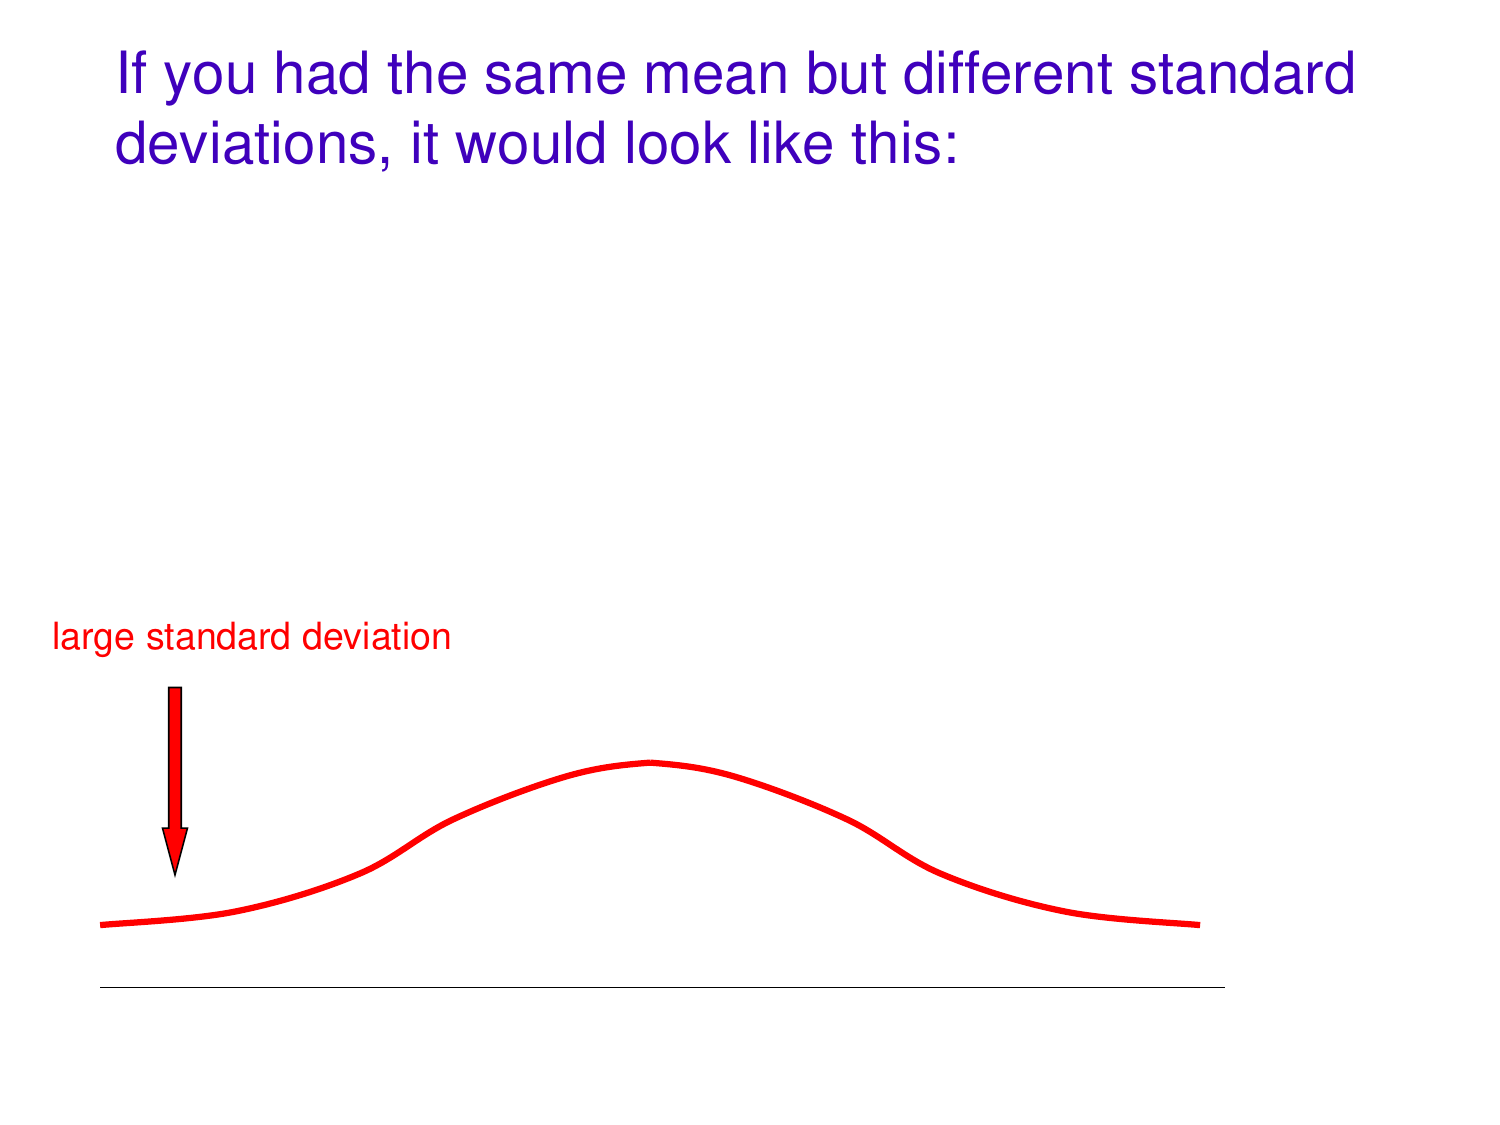
\includegraphics[width=0.65\textwidth]{assets/ch5-zelfde-sigma-verschillende-mu.png}
  \caption{Zelfde $\sigma$, verschillende $\mu$: de curve schuift naar links of rechts.}
\end{figure}

\begin{figure}[h!]
  \centering
  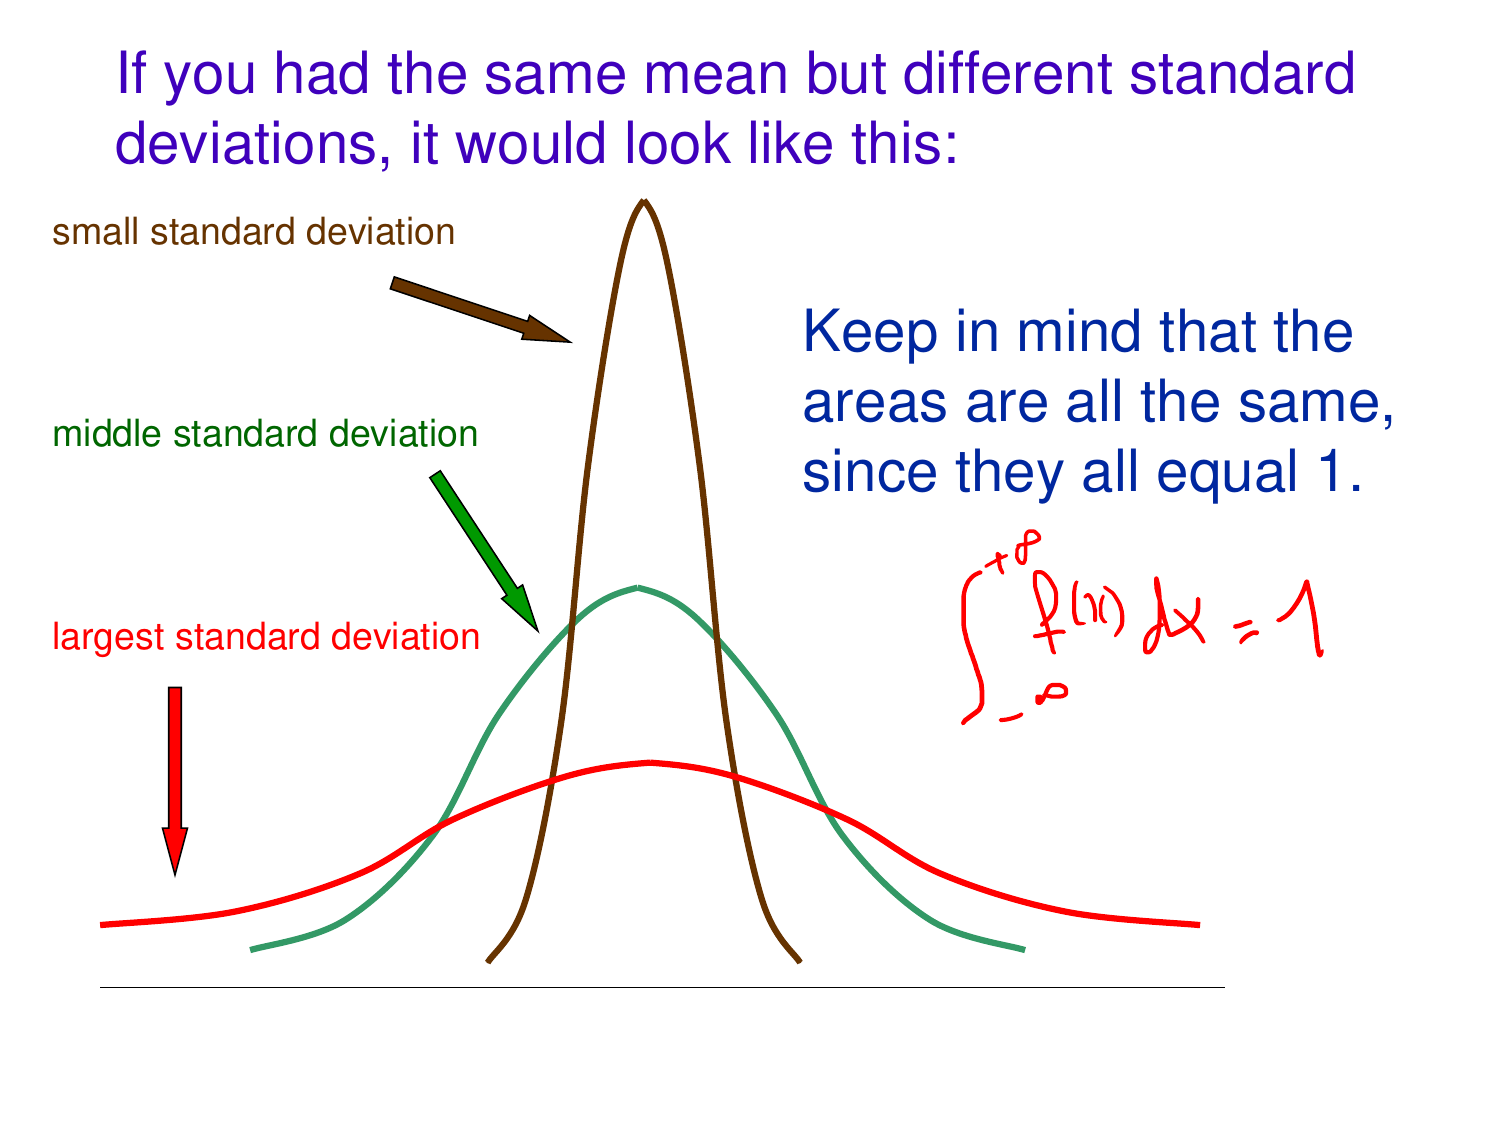
\includegraphics[width=0.65\textwidth]{assets/ch5-zelfde-mu-verschillende-sigma.png}
  \caption{Zelfde $\mu$, verschillende $\sigma$: grotere $\sigma$ = bredere, lagere curve. Oppervlakte blijft altijd 1.}
\end{figure}

\begin{conceptbox}[Eigenschappen van de normale verdeling]
\begin{itemize}
  \item Klokvormig en \emph{symmetrisch} rond $\mu$ -- de linker- en rechterhelft zijn spiegelbeelden.
  \item \emph{Grotere} $\sigma$ = bredere, lagere curve (meer spreiding).
  \item \emph{Kleinere} $\sigma$ = smallere, hogere curve (data geconcentreerder rond $\mu$).
  \item De totale oppervlakte is altijd 1, ongeacht $\mu$ en $\sigma$.
  \item De empirische 68-95-99,7\%-regel geldt voor \emph{elke} normale verdeling.
\end{itemize}
\end{conceptbox}

\subsection{5.3 -- Standaard Normale verdeling en kansen berekenen}

\begin{conceptbox}[Het probleem en de oplossing]
Er zijn oneindig veel normale verdelingen (één voor elk paar $\mu, \sigma$). Om kansen te kunnen berekenen zonder voor elke combinatie een andere tabel te maken, standaardiseren we alles naar \emph{één} vaste verdeling: de \textbf{standaard normale verdeling} met $\mu = 0$ en $\sigma = 1$.
\end{conceptbox}

\frm{Omzetting naar standaard normaal (z-score)}{z = \frac{x - \mu}{\sigma}}{%
  Als $x \sim \mathcal{N}(\mu, \sigma^2)$, dan is $z \sim \mathcal{N}(0, 1)$.\\
  De z-score zegt hoeveel standaardafwijkingen $x$ verwijderd is van $\mu$:\\
  $z = 1{,}5$ betekent: $x$ ligt 1,5 $\sigma$ boven het gemiddelde.}

\begin{theorieblok}[Stappenplan: kans berekenen voor normale variabele]
\begin{enumerate}
  \item \textbf{Schets} de normale verdeling, markeer $\mu$ en arceer het gewenste gebied.
  \item \textbf{Standardiseer}: bereken $z = \dfrac{x - \mu}{\sigma}$ voor elke grens.
  \item \textbf{Zoek} de oppervlakte op in de z-tabel (of Python: \texttt{sts.norm.cdf(z)}).
  \item \textbf{Gebruik symmetrie}: $P(z < -a) = P(z > a) = 1 - P(z < a)$.\\
  Elke helft heeft oppervlakte 0{,}5, dus $P(z > 0) = 0{,}5$.
\end{enumerate}
\textit{Voorbeeld:} $x \sim \mathcal{N}(10, 1{,}5^2)$, gevraagd $P(8 < x < 12)$:\\
$z_1 = (8-10)/1{,}5 = -1{,}33$ en $z_2 = (12-10)/1{,}5 = 1{,}33$\\
$P(-1{,}33 < z < 1{,}33) = 1 - 2 \cdot P(z < -1{,}33) = 1 - 2 \cdot 0{,}0918 = 0{,}8164$
\end{theorieblok}

\begin{figure}[h!]
  \centering
  
\includegraphics[width=0.60\textwidth]{assets/z-score-oefening.png}
  \caption{Voorbeeld z-score berekening: het arceerde gebied is de gevraagde kans.}
\end{figure}


\begin{pyblock}
from scipy import stats as sts

# Willekeurige normaalverdeling X ~ N(mu, sigma^2)
mu, sigma = 70, 10
rv = sts.norm(loc=mu, scale=sigma)

print(rv.cdf(80))                  # P(X <= 80)
print(rv.sf(80))                   # P(X > 80) = 1 - cdf(80)
print(rv.cdf(80) - rv.cdf(60))    # P(60 < X < 80)
print(rv.ppf(0.95))                # 95e percentiel (inverse CDF)

# Standaard normaal Z ~ N(0,1):
z = sts.norm(0, 1)
print(z.cdf(1.96))                 # 0.9750
print(z.ppf(0.975))                # 1.96
print(z.ppf(0.005))                # -2.576 (voor alpha=0.01 tweezijdig)
\end{pyblock}
\subsection{5.4 -- Normaliteit beoordelen}

\begin{conceptbox}[Waarom controleren we normaliteit?]
Veel statistische technieken (t-testen, betrouwbaarheidsintervallen voor kleine steekproeven\ldots) veronderstellen dat de data normaal verdeeld is. Als die aanname niet klopt, zijn de resultaten onbetrouwbaar. Hieronder staan 4 manieren om dit te controleren.
\end{conceptbox}

\begin{figure}[h!]
  \centering
  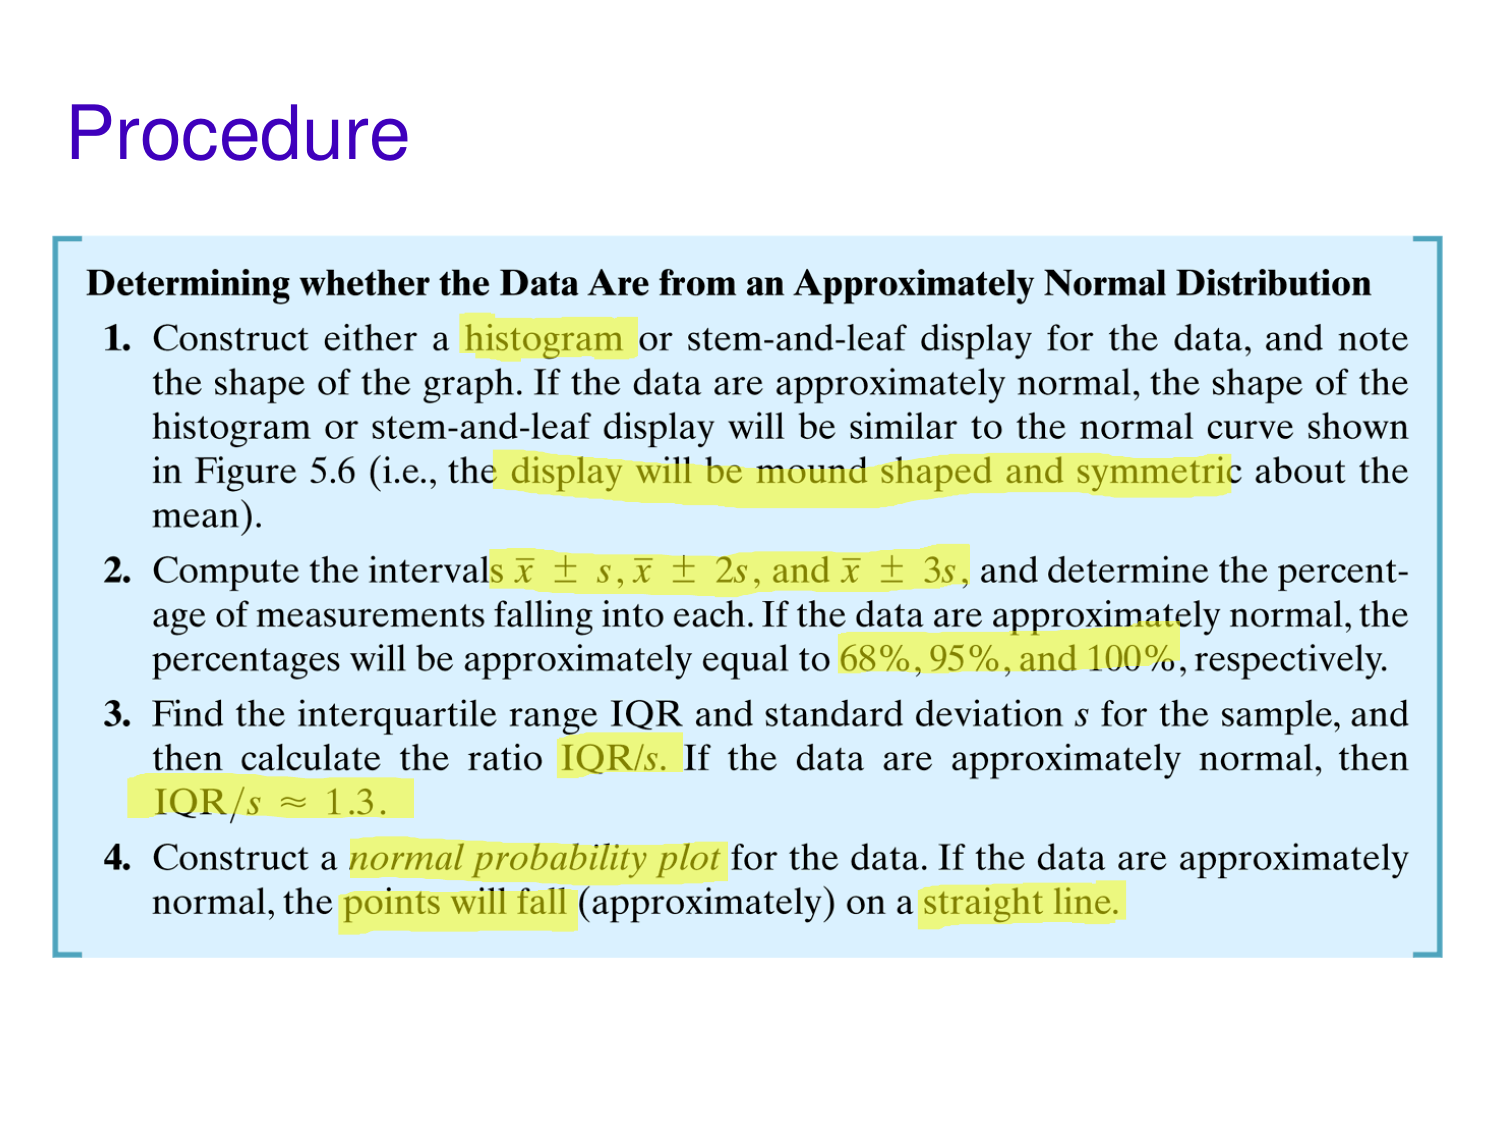
\includegraphics[width=0.72\textwidth]{assets/ch5-normaliteit-beoordelen.png}
  \caption{Stappenplan om normaliteit te beoordelen (uit de slides).}
\end{figure}

\begin{theorieblok}[4 manieren om normaliteit te controleren]
\begin{enumerate}
  \item \textbf{Histogram} -- moet klokvormig en symmetrisch zijn (geen duidelijke scheefheid).
  \item \textbf{Empirische regel} -- bereken $\bar{x} \pm s$, $\bar{x} \pm 2s$, $\bar{x} \pm 3s$ en controleer of $\approx 68\%$, $95\%$, $99{,}7\%$ van de data erin valt.
  \item \textbf{IQR/s-ratio} -- bereken $\dfrac{\text{IQR}}{s}$. Bij een normale verdeling is dit $\approx 1{,}3$.
  \item \textbf{Normal probability plot} -- plot de gesorteerde datapunten op de y-as versus de verwachte z-scores van een normale verdeling op de x-as. Als de punten \emph{op een rechte lijn} liggen, is de data normaal verdeeld.
\end{enumerate}
\end{theorieblok}

\subsection{5.4 -- Benadering Binomiaal via Normaal}

\begin{conceptbox}[Wanneer is dit nuttig?]
De binomiale formule wordt rekenintensief bij grote $n$. Gelukkig benadert de binomiale verdeling voor grote $n$ een normale verdeling met $\mu = np$ en $\sigma = \sqrt{npq}$. Je moet dan wel een kleine correctie toepassen omdat je een discrete verdeling benadert met een continue.
\end{conceptbox}

\begin{theorieblok}[Stappenplan: normale benadering van de binomiale verdeling]
\begin{enumerate}
  \item Controleer of $np \pm 3\sqrt{npq}$ volledig binnen $[0, n]$ valt -- zo niet, werkt de benadering slecht.
  \item Schrijf de gevraagde kans als $P(x \leq a)$ of een verschil ervan.
  \item Pas de \textbf{continuiteitscorrectie} toe: vervang $a$ door $(a + 0{,}5)$ (je vult het ``gat'' op tussen de discrete waarden).
  \item Bereken de z-waarde: $z = \dfrac{(a + 0{,}5) - np}{\sqrt{npq}}$.
\end{enumerate}
\end{theorieblok}

\subsection{5.5 -- Twee stochastische variabelen: Joint distributies}

Soms wil je twee variabelen \emph{tegelijk} bestuderen -- bv.\ het aantal GSM-balken ($x_1$) en de reactietijd in seconden ($x_2$). Dan heb je een \textbf{joint (gezamenlijke) kansverdeling} nodig.

\begin{figure}[h!]
  \centering
  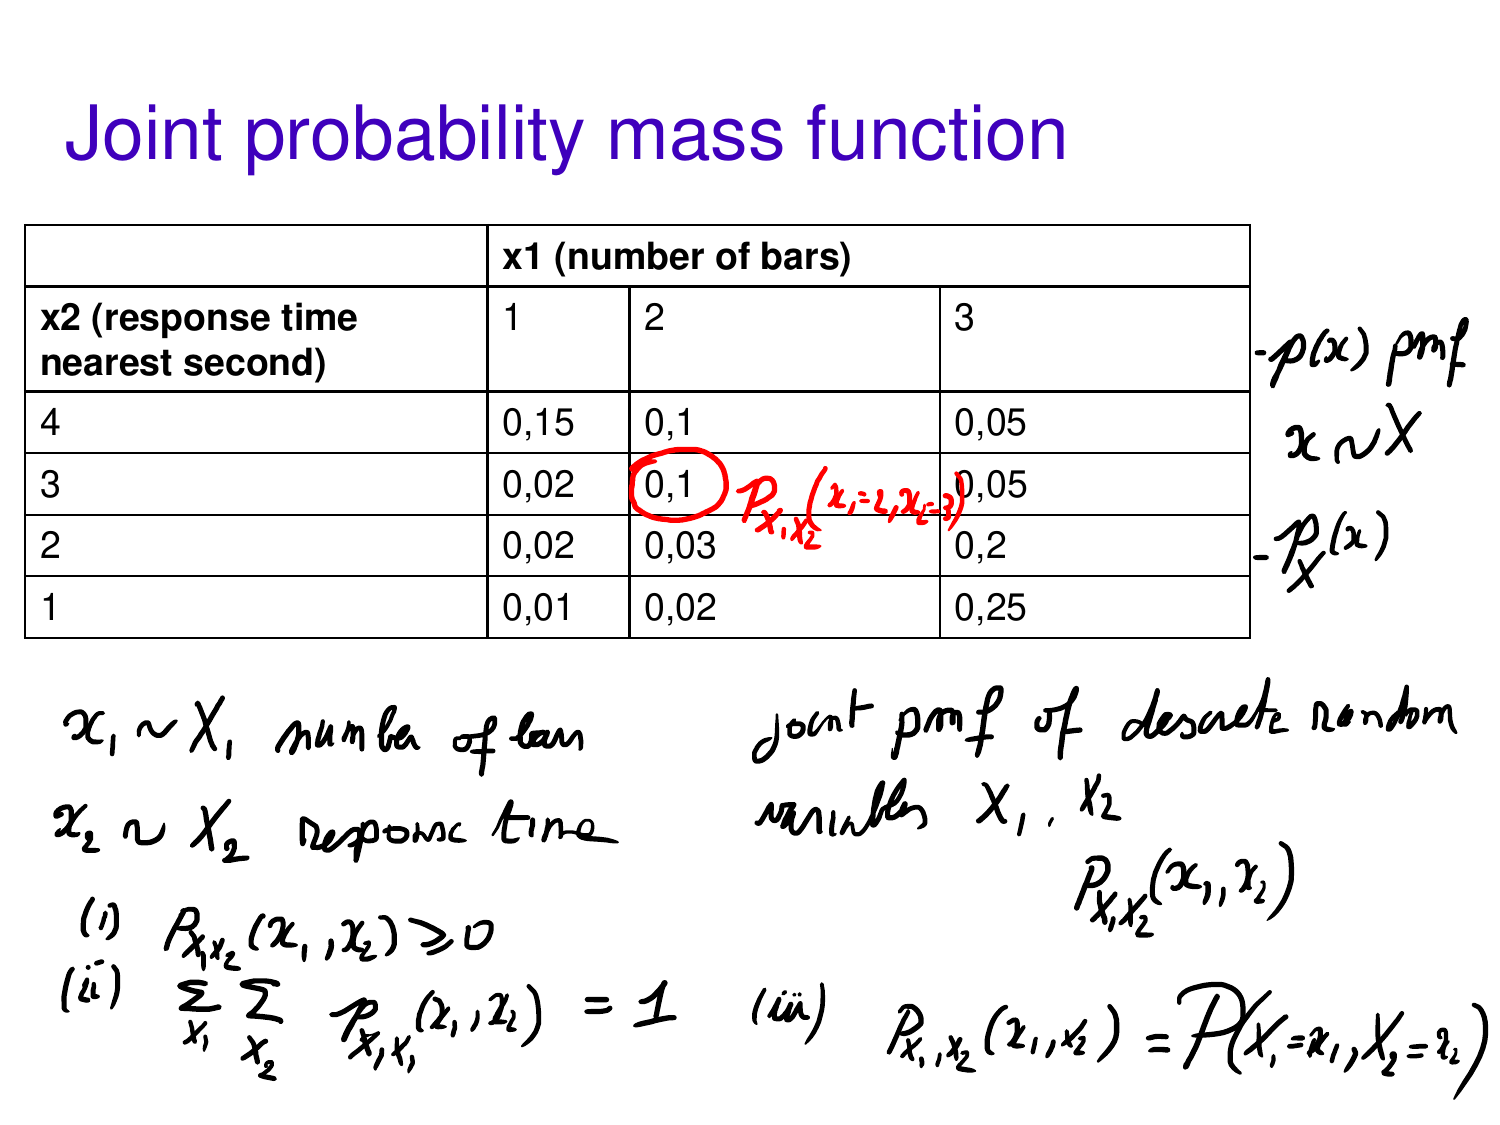
\includegraphics[width=0.68\textwidth]{assets/ch5-joint-pmf-tabel.png}
  \caption{Joint PMF in tabelvorm: rijen = $x_2$, kolommen = $x_1$. Elke cel = $p(x_1, x_2)$.}
\end{figure}

\begin{conceptbox}[Joint PMF en PDF]
\begin{itemize}
  \item \textbf{Joint PMF} (discreet): $p(x_1, x_2)$ = kans dat $x_1$ én $x_2$ gelijktijdig die waarden aannemen. Alle kansen samen sommeren tot 1.
  \item \textbf{Joint PDF} (continu): $f(x_1, x_2)$ -- kansen zijn dubbelintegralen over een 2D-gebied.
\end{itemize}
\end{conceptbox}

\begin{figure}[h!]
  \centering
  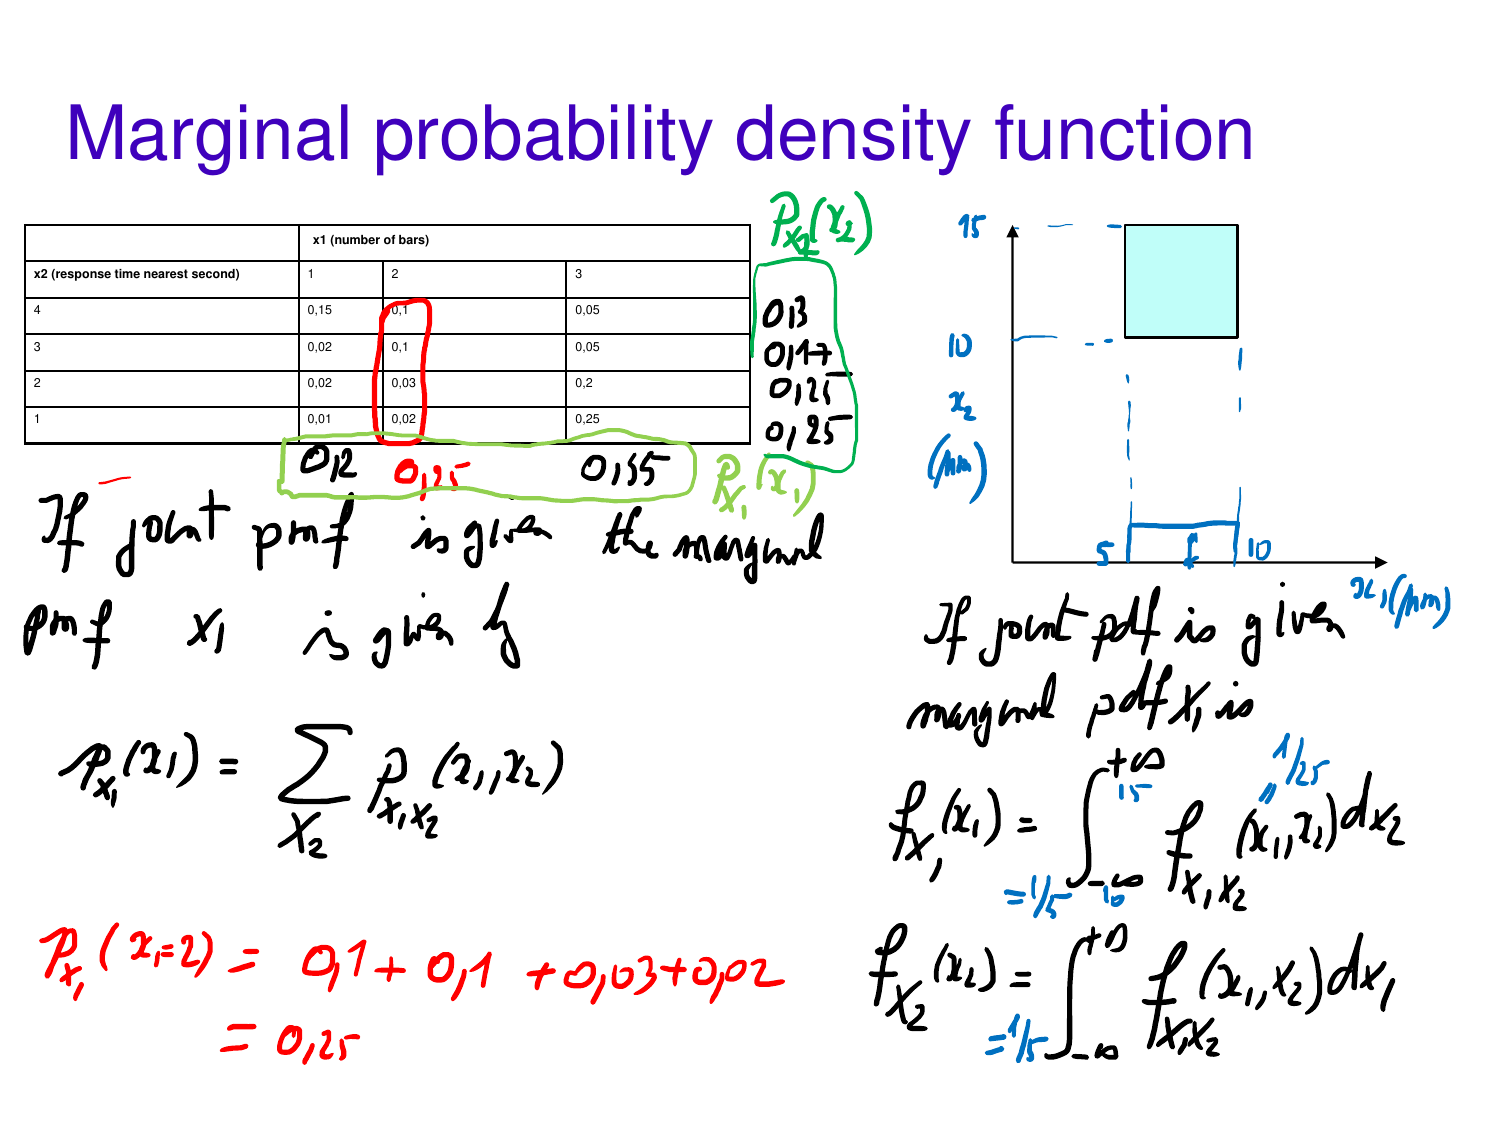
\includegraphics[width=0.65\textwidth]{assets/ch5-marginale-verdeling.png}
  \caption{De marginale verdeling van $x_1$: sommeer over alle waarden van $x_2$ (rijsommen of kolomsommen).}
\end{figure}

\begin{conceptbox}[Marginale kansverdeling]
Als je alleen geïnteresseerd bent in één variabele, ``marginaliseer'' je de andere weg -- je telt gewoon over alle waarden van de andere variabele:
\[p_1(x_1) = \sum_{\text{alle } x_2} p(x_1, x_2) \qquad \text{(discreet)} \qquad f_1(x_1) = \int_{-\infty}^{+\infty} f(x_1, x_2)\,dx_2 \qquad \text{(continu)}\]
Dit zijn de \emph{kolomsommen} (of rijtotalen) van de joint PMF-tabel.
\end{conceptbox}

\begin{figure}[h!]
  \centering
  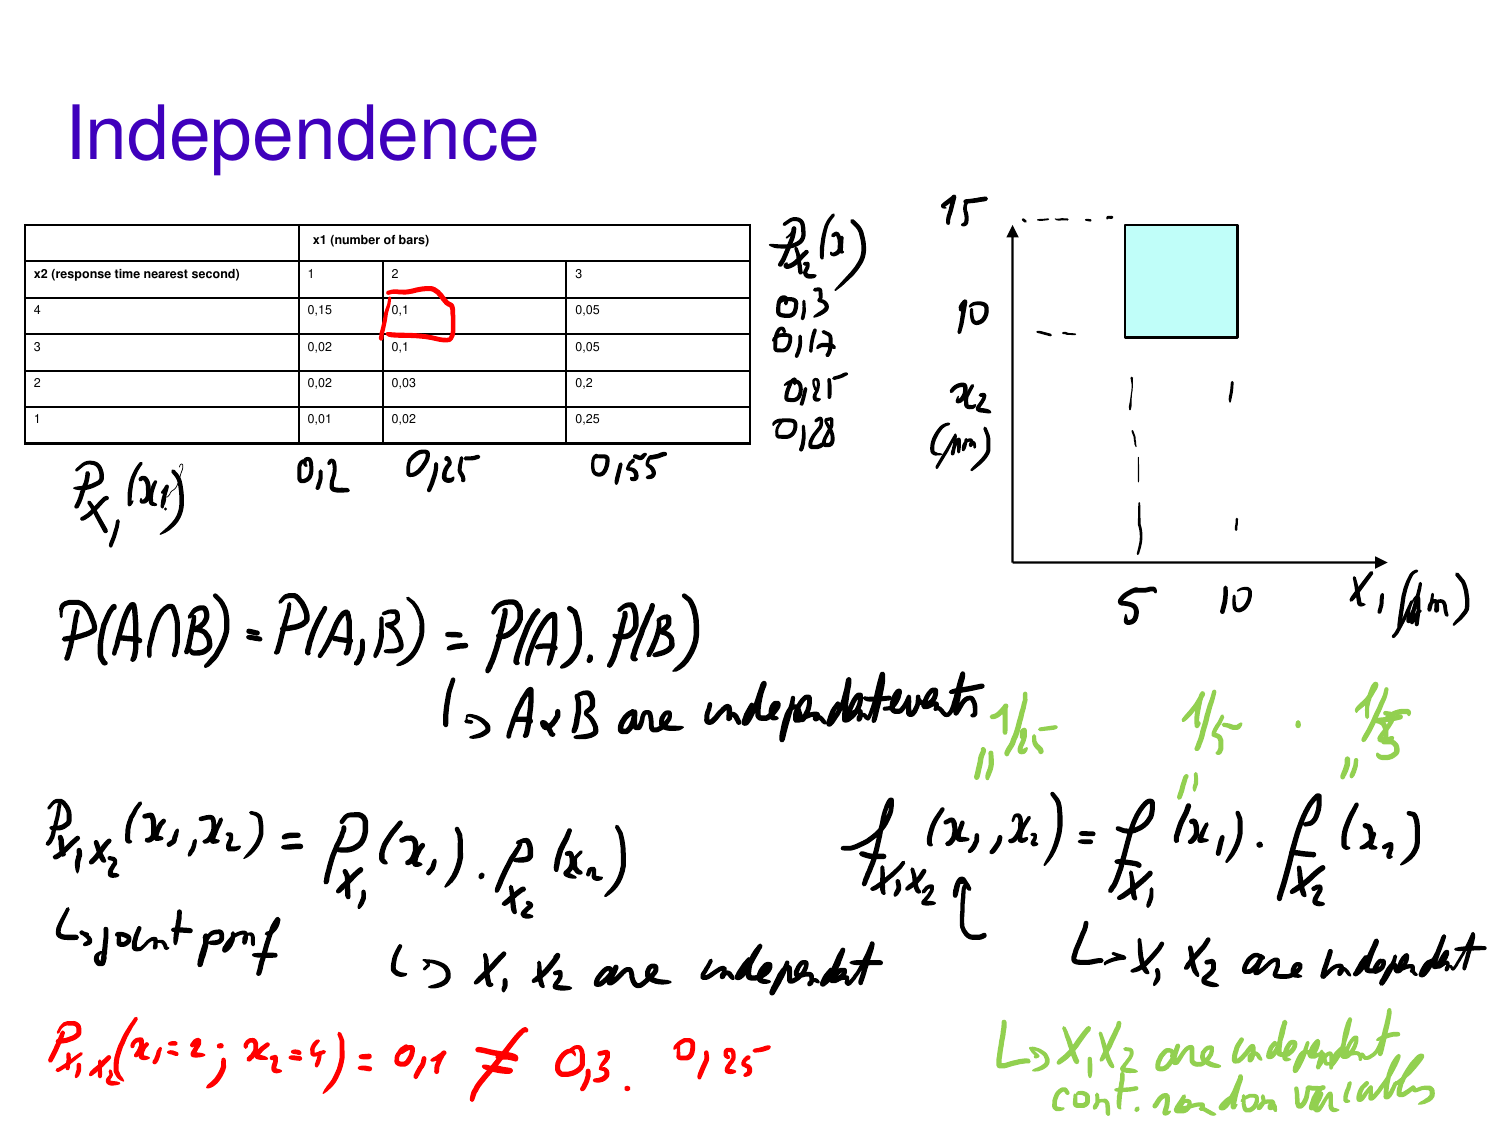
\includegraphics[width=0.68\textwidth]{assets/ch5-onafhankelijkheid-2var.png}
  \caption{Onafhankelijkheidscontrole: is $p(x_1, x_2) = p_1(x_1) \cdot p_2(x_2)$ voor elke combinatie?}
\end{figure}

\begin{conceptbox}[Onafhankelijkheid van twee variabelen]
$x_1$ en $x_2$ zijn \textbf{onafhankelijk} als de joint PMF gelijk is aan het product van de marginale PMFs voor \emph{alle} combinaties:
\[p(x_1, x_2) = p_1(x_1) \cdot p_2(x_2) \quad \forall (x_1, x_2)\]
Praktisch: bereken $p_1(x_1) \cdot p_2(x_2)$ voor elke cel en vergelijk met de tabel. Als ook maar één cel niet klopt, zijn ze afhankelijk.
\end{conceptbox}

\subsection{5.5 -- Covariantie}

\begin{figure}[h!]
  \centering
  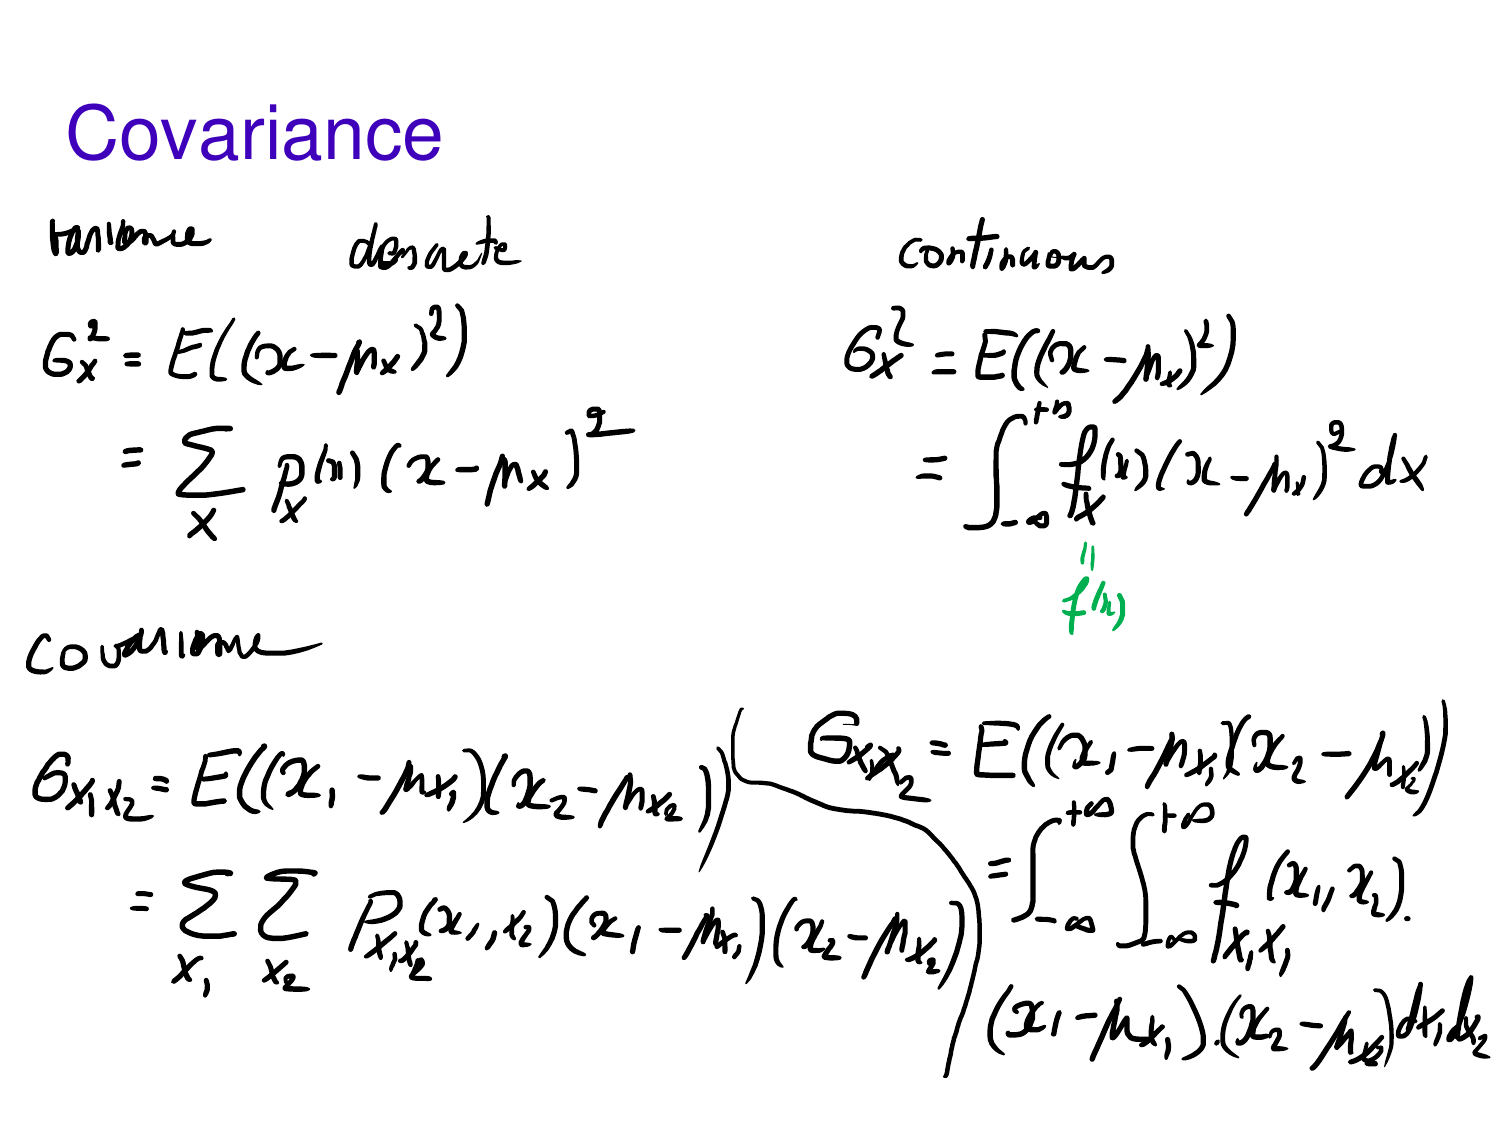
\includegraphics[width=0.68\textwidth]{assets/ch5-covariantie.png}
  \caption{Formule en interpretatie van de covariantie uit de slides.}
\end{figure}

\frm{Covariantie}{\sigma_{12} = \text{Cov}(x_1, x_2) = E\!\left[(x_1-\mu_1)(x_2-\mu_2)\right]}{%
  Voor discrete variabelen: $\sigma_{12} = \sum_{x_1}\sum_{x_2}(x_1-\mu_1)(x_2-\mu_2)\,p(x_1,x_2)$.\\
  $\sigma_{12} > 0$: positieve samenhang (beide stijgen samen). \quad
  $\sigma_{12} < 0$: negatieve samenhang. \quad
  $\sigma_{12} = 0$: geen lineaire samenhang.}

\begin{conceptbox}[$\sigma_{12}$ -- Covariantie]
\sym{sigmatwaalfnl}{Covariantie van $x_1$ en $x_2$ ($\sigma_{12}$)}{--}
\textbf{Interpretatie:}
\begin{itemize}
  \item $\sigma_{12} > 0$: als $x_1$ boven $\mu_1$ ligt, is $x_2$ ook vaak boven $\mu_2$ -- \emph{positieve} samenhang.
  \item $\sigma_{12} < 0$: als $x_1$ boven $\mu_1$ ligt, is $x_2$ vaak onder $\mu_2$ -- \emph{negatieve} samenhang.
  \item $\sigma_{12} = 0$: geen lineaire samenhang (maar de variabelen kunnen nog afhankelijk zijn op een niet-lineaire manier!).
\end{itemize}
\end{conceptbox}

\subsection{5.6 -- Bivariate Gaussiaanse verdeling}

De \textbf{bivariate Gaussiaan} is de 2D-versie van de normale verdeling. In plaats van een klokvorm in 1D, krijg je een ``klokvormige heuvel'' in 2D.

\begin{conceptbox}[Bivariate Gaussiaan]
\[\mathbf{x} = \begin{pmatrix}x_1\\x_2\end{pmatrix} \sim \mathcal{N}(\boldsymbol{\mu},\,\boldsymbol{\Sigma}) \qquad \text{met} \qquad \boldsymbol{\mu} = \begin{pmatrix}\mu_1\\\mu_2\end{pmatrix},\quad \boldsymbol{\Sigma} = \begin{pmatrix}\sigma_1^2 & \sigma_{12}\\ \sigma_{12} & \sigma_2^2\end{pmatrix}\]
$\boldsymbol{\Sigma}$ is de \textbf{covariantiematrix}: symmetrisch en semi-positief definiet (alle eigenwaarden $\geq 0$).
De ``hoogtelijnen'' (isocontours) zijn ellipsen.
\end{conceptbox}

\frm{Bivariate Gaussiaanse PDF}{f(\mathbf{x}) = \frac{1}{2\pi\|\boldsymbol{\Sigma}\|^{1/2}}\exp\!\left(-\tfrac{1}{2}(\mathbf{x}-\boldsymbol{\mu})^T\boldsymbol{\Sigma}^{-1}(\mathbf{x}-\boldsymbol{\mu})\right)}{}

\begin{conceptbox}[Effect van de covariantiematrix op de vorm]
\begin{itemize}
  \item \textbf{Diagonale $\boldsymbol{\Sigma}$} ($\sigma_{12} = 0$): $x_1$ en $x_2$ zijn onafhankelijk -- de ellipsen zijn evenwijdig met de assen.
  \item \textbf{Positieve off-diagonaal} ($\sigma_{12} > 0$): de ellipsen kantelen rechtsboven/linksonder -- als $x_1$ stijgt, stijgt $x_2$ ook.
  \item \textbf{Negatieve off-diagonaal} ($\sigma_{12} < 0$): omgekeerde kanteling -- als $x_1$ stijgt, daalt $x_2$.
  \item De diagonaalelementen $\sigma_1^2$ en $\sigma_2^2$ bepalen de \emph{breedte} van de ellips langs elke as.
\end{itemize}
\end{conceptbox}

\subsection{5.7 -- Lineaire combinaties van stochastische variabelen}

\begin{conceptbox}[Wat is een lineaire combinatie?]
Als je twee onafhankelijke metingen hebt (bv.\ gewicht van twee pakketten), en je wilt de totale verwachting en spreiding berekenen, gebruik je de regels voor lineaire combinaties.
Stel $y = a_1 x_1 + a_2 x_2 + \cdots + a_k x_k$.
\end{conceptbox}

\frm{Gemiddelde van lineaire combinatie}{E(y) = a_1\mu_1 + a_2\mu_2 + \cdots + a_k\mu_k}{%
  Altijd geldig, ongeacht onafhankelijkheid.}

\frm{Variantie van lineaire combinatie (onafhankelijke $x_i$)}{\sigma_y^2 = a_1^2\sigma_1^2 + a_2^2\sigma_2^2 + \cdots + a_k^2\sigma_k^2}{%
  Enkel geldig als $x_1, x_2, \ldots, x_k$ \emph{onafhankelijk} zijn. Let op: de varianties tellen op, de standaardafwijkingen s\emph{niet}!}

\newpage
% =============================================================================
%  HOOFDSTUK 6: SAMPLING DISTRIBUTIONS (VERDELING VAN STEEKPROEFGROOTHEDEN)
% =============================================================================
\section{Ch.\ 6 -- Sampling Distributions (Verdeling van steekproefgrootheden)}

In de vorige hoofdstukken werkten we met de verdeling van individuele meetwaarden $x$. Nu gaan we een stap verder: wat als je telkens een \emph{steekproef} neemt en het \emph{gemiddelde} berekent? Dat gemiddelde is zelf ook een stochastische variabele met een eigen verdeling -- de \textbf{steekproefverdeling}.

\begin{conceptbox}[Parameter vs.\ Steekproefgrootheid]
\begin{itemize}
  \item \textbf{Parameter} -- een getal dat de \emph{populatie} beschrijft, bv.\ $\mu$ (populatiegemiddelde) of $\sigma^2$ (populatievariantie). Je kent dit getal meestal \emph{niet}.
  \item \textbf{Steekproefgrootheid (sample statistic)} -- een getal berekend uit de \emph{steekproef}, bv.\ $\bar{x}$ (steekproefgemiddelde) of $s^2$ (steekproefvariantie). Je gebruikt dit als \emph{schatting} voor de parameter.
\end{itemize}
Omdat elke nieuwe steekproef andere waarden geeft, is een steekproefgrootheid zelf een \emph{stochastische variabele} -- ze heeft een kansverdeling, een gemiddelde en een standaardafwijking.
\end{conceptbox}

\begin{figure}[h!]
  \centering
  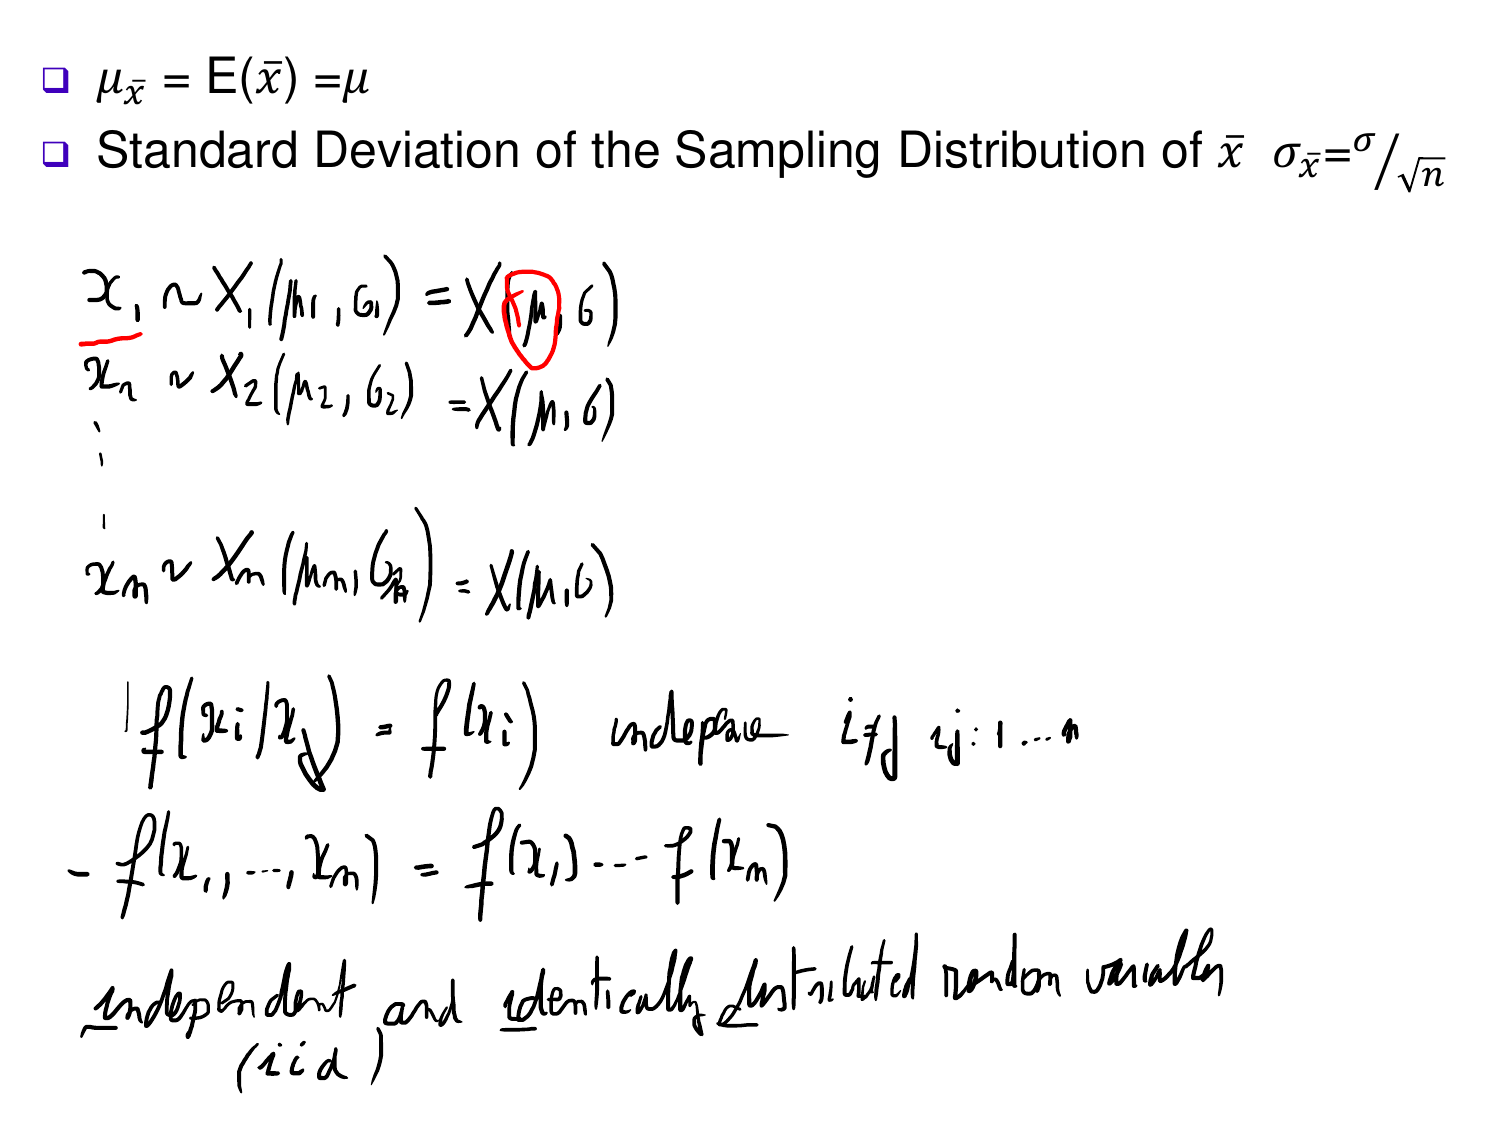
\includegraphics[width=0.72\textwidth]{assets/ch6-sampling-dist-eigenschappen.png}
  \caption{De twee sleuteleigenschappen van de steekproefverdeling van $\bar{x}$ (uit de slides).}
\end{figure}

\subsection{6.1 -- Eigenschappen van de steekproefverdeling van $\bar{x}$}

\begin{theorieblok}[De twee fundamentele eigenschappen]
Stel dat je herhaaldelijk steekproeven van grootte $n$ trekt uit een populatie met gemiddelde $\mu$ en standaardafwijking $\sigma$. Dan geldt voor de steekproefverdeling van $\bar{x}$:

\textbf{Eigenschap 1 -- Het gemiddelde:}
\[\mu_{\bar{x}} = E(\bar{x}) = \mu\]
Het gemiddelde van alle mogelijke steekproefgemiddelden is gelijk aan het populatiegemiddelde. Dit betekent dat $\bar{x}$ een \textbf{zuivere schatting} (\emph{unbiased estimator}) is van $\mu$ -- gemiddeld gezien zit je er niet naast.

\textbf{Eigenschap 2 -- De standaardfout:}
\[\sigma_{\bar{x}} = \frac{\sigma}{\sqrt{n}}\]
De spreiding van de steekproefgemiddelden neemt af als $n$ groeit. Bij grotere steekproeven liggen alle $\bar{x}$-waarden dichter bij $\mu$. Deze $\sigma_{\bar{x}}$ noemen we de \textbf{standaardfout van het gemiddelde}.
\end{theorieblok}

\frm{Standaardfout van het gemiddelde}{\sigma_{\bar{x}} = \frac{\sigma}{\sqrt{n}}}{%
  $\sigma_{\bar{x}}$ = standaardfout van het gemiddelde (standaardafwijking van de steekproefverdeling van $\bar{x}$).\\
  Hoe groter $n$, hoe kleiner de standaardfout en hoe betrouwbaarder de schatting.}

\begin{figure}[h!]
  \centering
  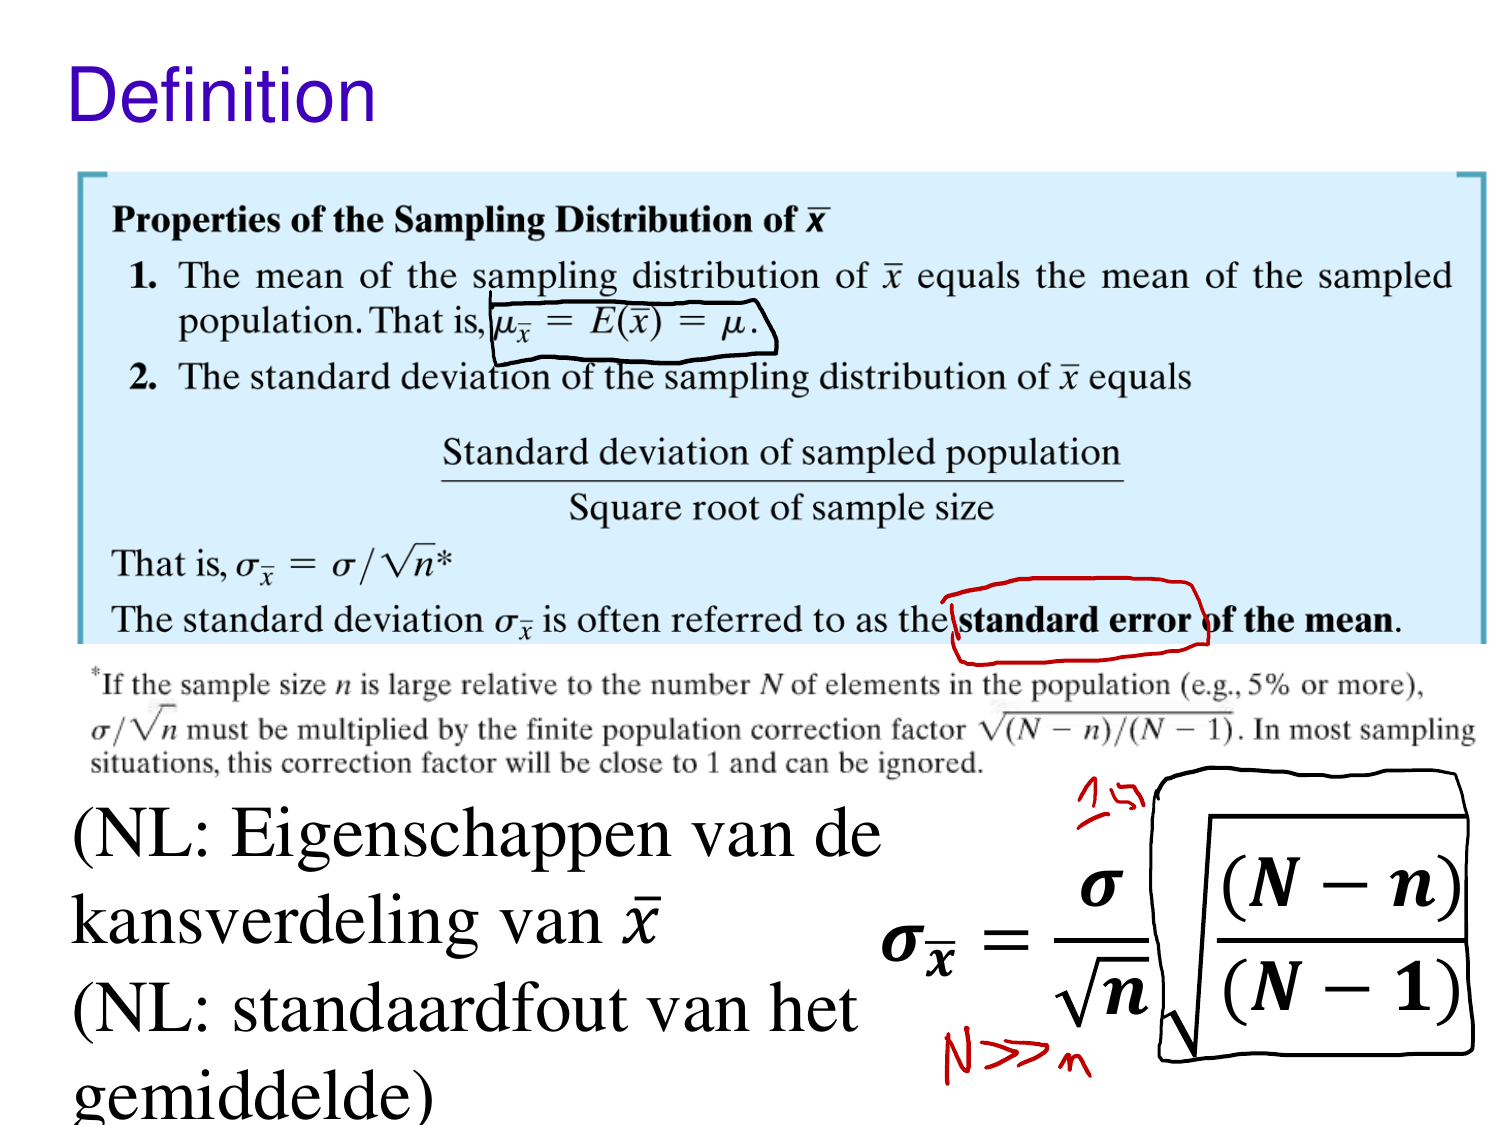
\includegraphics[width=0.72\textwidth]{assets/ch6-standaardfout-correctie.png}
  \caption{Correctiefactor voor eindige populaties: wanneer $n$ groot is t.o.v.\ $N$.}
\end{figure}

\begin{conceptbox}[Correctiefactor voor eindige populatie]
Als de populatie \emph{eindig} is (grootte $N$) en de steekproef $n$ is meer dan ~5\% van $N$, gebruik dan:
\[\sigma_{\bar{x}} = \frac{\sigma}{\sqrt{n}} \cdot \sqrt{\frac{N-n}{N-1}}\]
De factor $\sqrt{\frac{N-n}{N-1}}$ heet de \textbf{eindige populatiecorrectiefactor}. Ze is kleiner dan 1 en maakt de standaardfout kleiner -- logisch, want als je bijna de hele populatie hebt gemeten, weet je het bijna zeker.
\end{conceptbox}

\begin{conceptbox}[Zuivere schatting vs.\ scheve schatting]
\begin{itemize}
  \item \textbf{Zuivere schatting (unbiased)} -- het gemiddelde van de steekproefverdeling = de populatieparameter. $\bar{x}$ is een zuivere schatting van $\mu$.
  \item \textbf{Scheve schatting (biased)} -- het gemiddelde van de steekproefverdeling $\neq$ de populatieparameter.
  \item \textbf{Minimum-variantie zuivere schatting} -- van alle zuivere schattingen is $\bar{x}$ degene met de \emph{kleinste variantie}. Dat maakt $\bar{x}$ de beste keuze om $\mu$ te schatten.
\end{itemize}
\end{conceptbox}

\subsection{6.2 -- De Centrale Limietstelling (CLT)}

De Centrale Limietstelling is één van de belangrijkste stellingen in de statistiek. Ze legt uit waarom de normale verdeling zo vaak opduikt in de natuur.

\begin{figure}[h!]
  \centering
  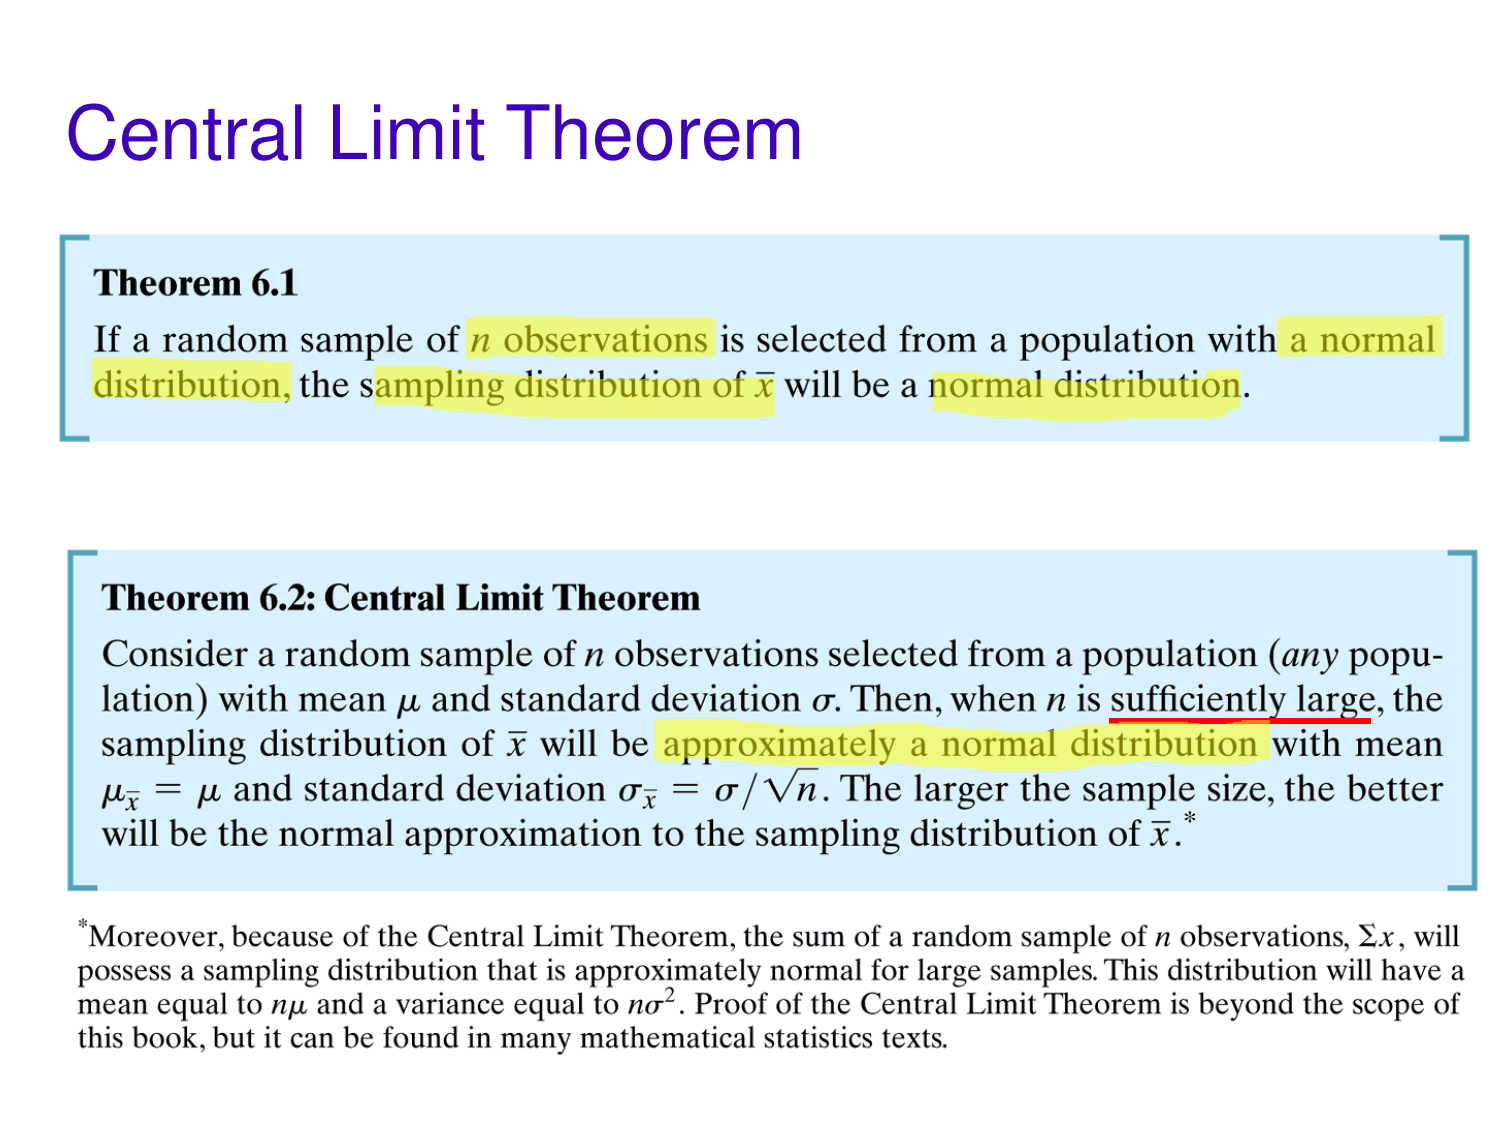
\includegraphics[width=0.72\textwidth]{assets/ch6-centrale-limietstelling.png}
  \caption{De formele definitie van de Centrale Limietstelling (uit de slides).}
\end{figure}

\begin{theorieblok}[Centrale Limietstelling (CLT)]
Beschouw een willekeurige steekproef van $n$ observaties uit een populatie met gemiddelde $\mu$ en standaardafwijking $\sigma$.

\textbf{Voor normale populaties:} de steekproefverdeling van $\bar{x}$ is \emph{altijd} normaal verdeeld, ongeacht $n$.

\textbf{Voor elke andere populatie:} als $n$ groot genoeg is, is de steekproefverdeling van $\bar{x}$ \emph{bij benadering} normaal verdeeld:
\[\bar{x} \;\dot{\sim}\; \mathcal{N}\!\left(\mu,\; \frac{\sigma^2}{n}\right)\]
In beide gevallen kan je $\bar{x}$ standaardiseren als:
\[z = \frac{\bar{x} - \mu}{\sigma/\sqrt{n}}\]
\end{theorieblok}

\begin{figure}[h!]
  \centering
  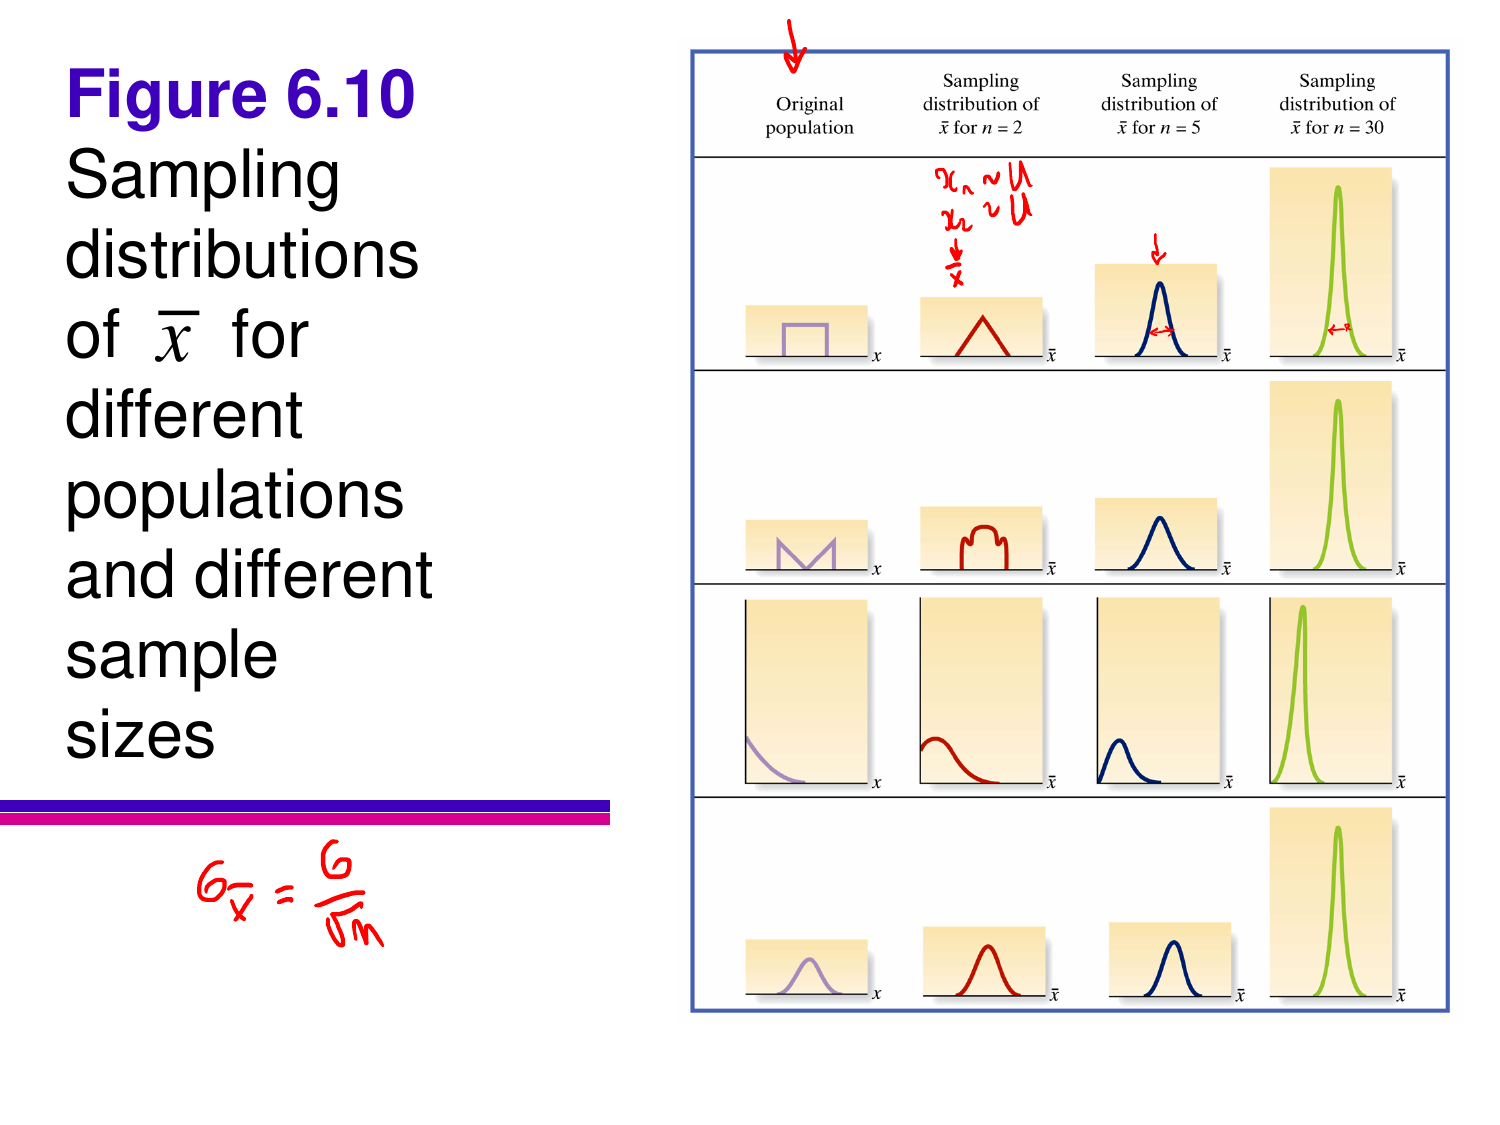
\includegraphics[width=0.72\textwidth]{assets/ch6-clt-verschillende-populaties.png}
  \caption{De CLT in actie: voor uniforme, scheve en normale populaties convergeert de verdeling van $\bar{x}$ steeds sneller naar normaal als $n$ toeneemt.}
\end{figure}

\begin{figure}[h!]
  \centering
  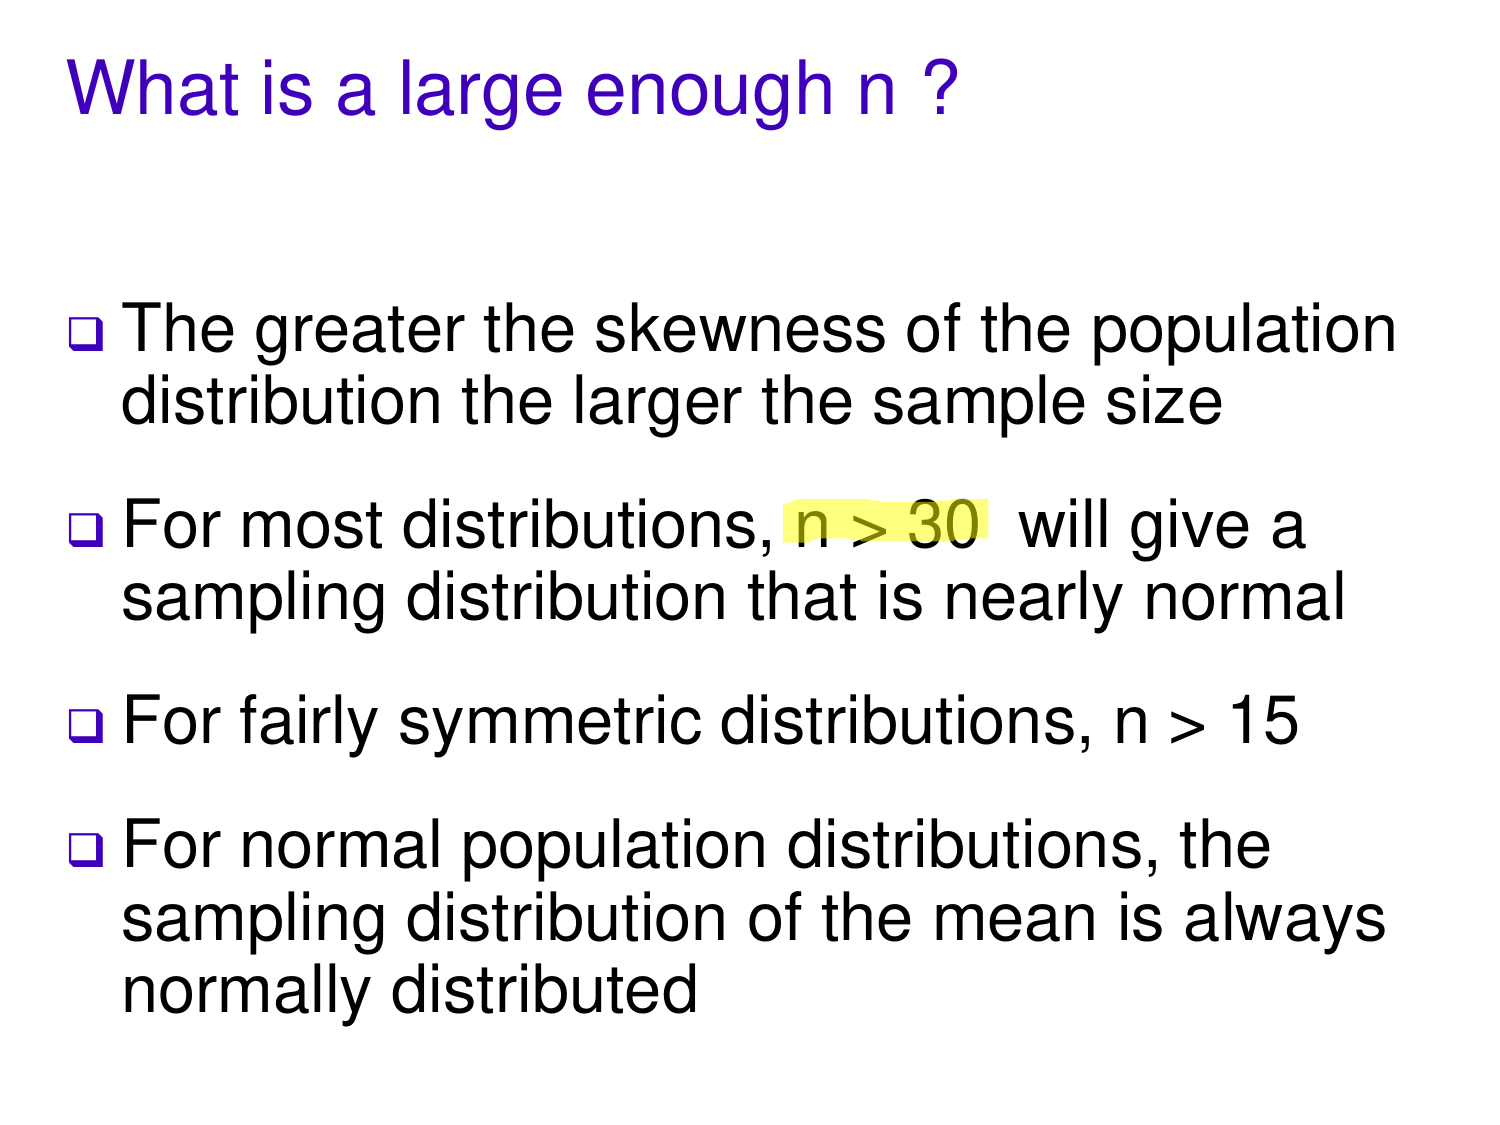
\includegraphics[width=0.72\textwidth]{assets/ch6-grote-n-vraag.png}
  \caption{Hoe groot moet $n$ zijn? Dat hangt af van de scheefheid van de populatie.}
\end{figure}

\begin{conceptbox}[Hoe groot moet $n$ zijn voor de CLT?]
\begin{itemize}
  \item \textbf{Normale populatie:} de steekproefverdeling is altijd normaal, voor elke $n$.
  \item \textbf{Vrij symmetrische populatie:} $n > 15$ is al voldoende.
  \item \textbf{Scheve populatie:} $n > 30$ geeft een bijna normale steekproefverdeling.
  \item \textbf{Sterk scheve populatie:} je hebt een nog grotere $n$ nodig.
\end{itemize}
\textit{Vuistregel:} gebruik $n > 30$ als je niet zeker bent van de verdeling van de populatie.
\end{conceptbox}

\begin{figure}[h!]
  \centering
  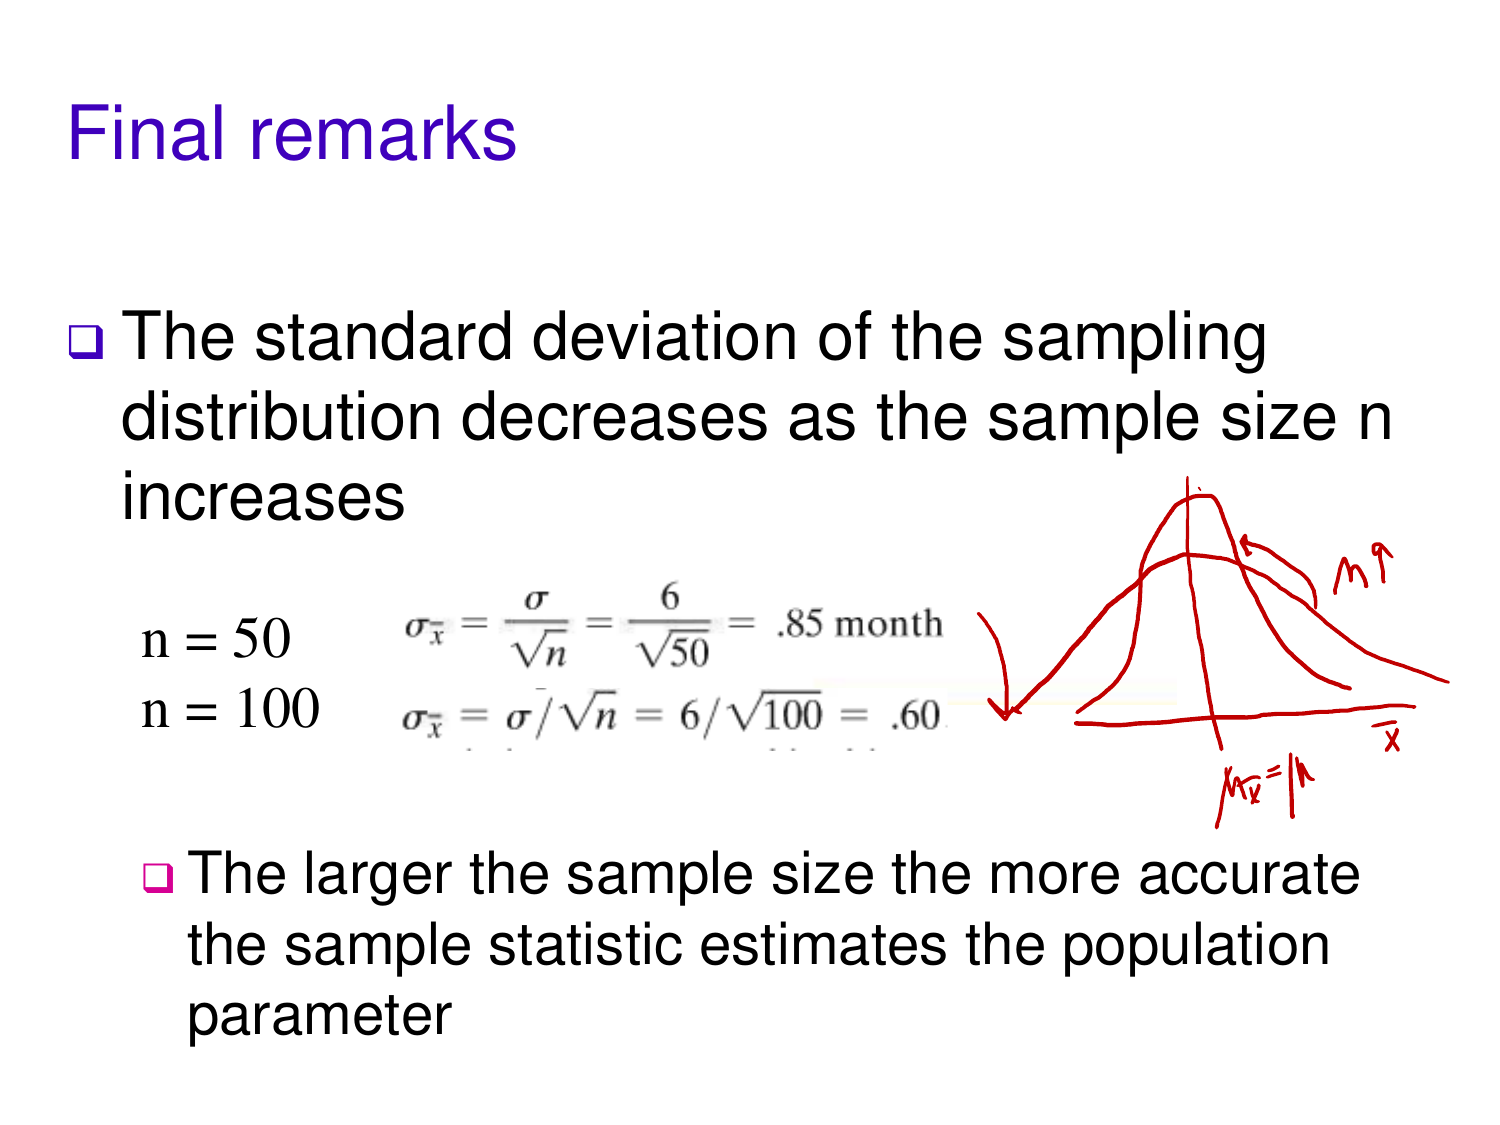
\includegraphics[width=0.68\textwidth]{assets/ch6-standaardfout-daalt.png}
  \caption{Naarmate $n$ groter wordt, worden de steekproefgemiddelden steeds dichter bij $\mu$ gegroepeerd.}
\end{figure}

\begin{examenbox}
\textbf{Intuïtie achter de CLT:} veel fenomenen in de natuur zijn de \emph{som} van vele kleine onafhankelijke bijdragen (bv.\ regenval = som van bijdragen van duizenden druppels). De CLT zegt dat zo'n som altijd normaal verdeeld wordt, ongeacht hoe de individuele bijdragen verdeeld zijn. Dát is waarom de normale verdeling overal opduikt.
\end{examenbox}

\newpage
% =============================================================================
%  HOOFDSTUK 7: BETROUWBAARHEIDSINTERVALLEN
% =============================================================================
\section{Ch.\ 7 -- Betrouwbaarheidsintervallen gebaseerd op één steekproef}

Tot nu toe leerden we hoe we $\mu$ kunnen \emph{schatten} met $\bar{x}$. Maar $\bar{x}$ is slechts een \emph{puntschatting} -- één enkel getal. In de praktijk wil je ook weten: \emph{hoe zeker ben ik?} Dat doen we met een \textbf{betrouwbaarheidsinterval}.

\begin{conceptbox}[Puntschatting vs.\ Intervalschatting]
\begin{itemize}
  \item \textbf{Puntschatting} -- één getal als schatting van de parameter, bv.\ $\bar{x} = 4{,}5$ dagen. Eenvoudig, maar geeft geen idee van de onzekerheid.
  \item \textbf{Intervalschatting (betrouwbaarheidsinterval)} -- een interval dat de parameter met een bepaalde kans bevat, bv.\ ``$\mu$ ligt met 95\% kans tussen 3{,}7 en 5{,}3 dagen''.
\end{itemize}
\end{conceptbox}

\subsection{7.1 -- Doelparameter bepalen}

Voor je een interval berekent, moet je weten \emph{welke} parameter je wilt schatten:

\begin{conceptbox}[Welke parameter schat je?]
\begin{itemize}
  \item \textbf{Gemiddelde $\mu$} -- sleutelwoorden: gemiddelde, mean, verwachting. Data is kwantitatief.
  \item \textbf{Proportie $p$} -- sleutelwoorden: fractie, percentage, verhouding, rate. Data is kwalitatief (ja/nee).
  \item \textbf{Variantie $\sigma^2$} -- sleutelwoorden: spreiding, variabiliteit. Data is kwantitatief.
\end{itemize}
\end{conceptbox}

\subsection{7.2 -- CI voor \texorpdfstring{$\mu$}{mu} met z-statistiek (grote steekproef, $n>30$)}

\begin{conceptbox}[De redenering achter het CI]
We weten (uit Ch.\ 6) dat voor grote $n$:
\[\bar{x} \sim \mathcal{N}\!\left(\mu,\, \frac{\sigma^2}{n}\right) \qquad \Rightarrow \qquad z = \frac{\bar{x} - \mu}{\sigma/\sqrt{n}} \sim \mathcal{N}(0,1)\]
Uit de z-tabel weten we dat $P(-1{,}96 < z < 1{,}96) = 0{,}95$. We draaien dit om:
\[P\!\left(\bar{x} - 1{,}96\,\frac{\sigma}{\sqrt{n}} < \mu < \bar{x} + 1{,}96\,\frac{\sigma}{\sqrt{n}}\right) = 0{,}95\]
Dat is ons 95\%-betrouwbaarheidsinterval!
\end{conceptbox}

\begin{figure}[h!]
  \centering
  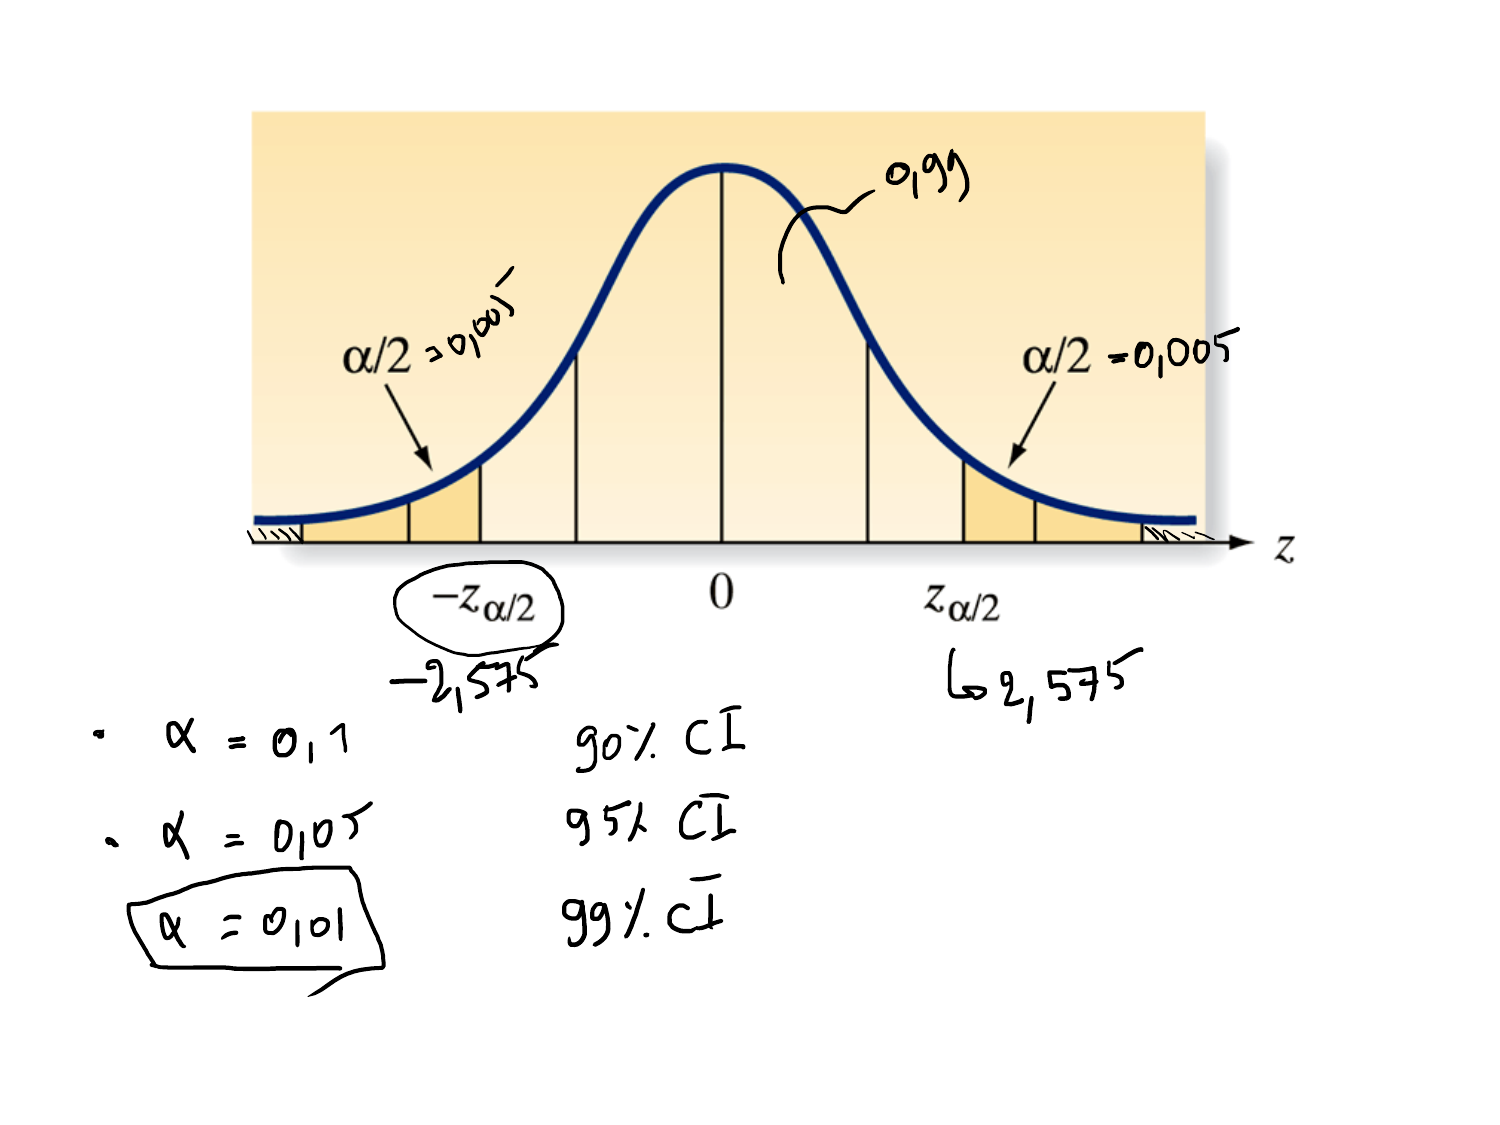
\includegraphics[width=0.68\textwidth]{assets/ch7-sampling-dist-xbar.png}
  \caption{De steekproefverdeling van $\bar{x}$ en hoe we de z-waarde gebruiken.}
\end{figure}

\begin{figure}[h!]
  \centering
  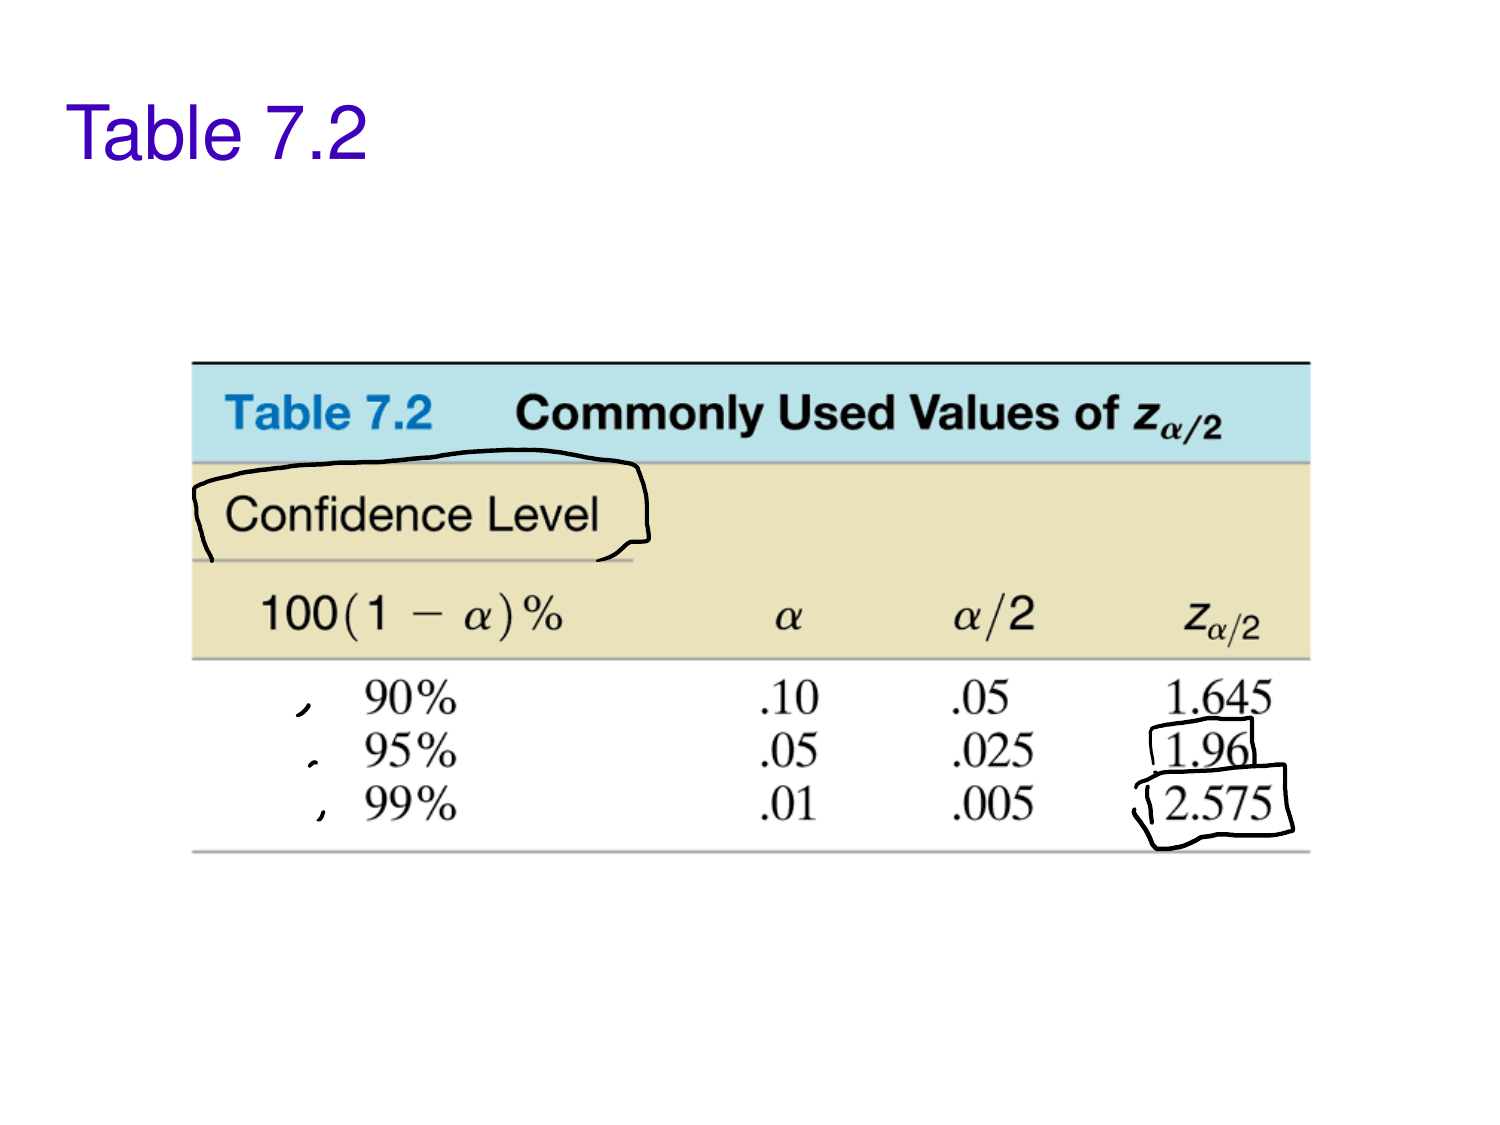
\includegraphics[width=0.68\textwidth]{assets/ch7-z-waarden-tabel.png}
  \caption{Veelgebruikte z-waarden voor betrouwbaarheidsintervallen.}
\end{figure}

\frm{Betrouwbaarheidsinterval voor $\mu$ (grote steekproef)}{\bar{x} \pm z_{\alpha/2} \cdot \frac{\sigma}{\sqrt{n}} \approx \bar{x} \pm z_{\alpha/2} \cdot \frac{s}{\sqrt{n}}}{%
  $z_{\alpha/2}$ = z-waarde zodat $P(z > z_{\alpha/2}) = \alpha/2$ (rechterstaart heeft oppervlak $\alpha/2$).\\
  Als $\sigma$ onbekend is (praktisch altijd), gebruik je $s$ als schatting. Geldig voor $n > 30$.\\
  Veelgebruikte waarden: $z_{0{,}025} = 1{,}96$ (95\% CI), $z_{0{,}005} = 2{,}575$ (99\% CI).}

\begin{figure}[h!]
  \centering
  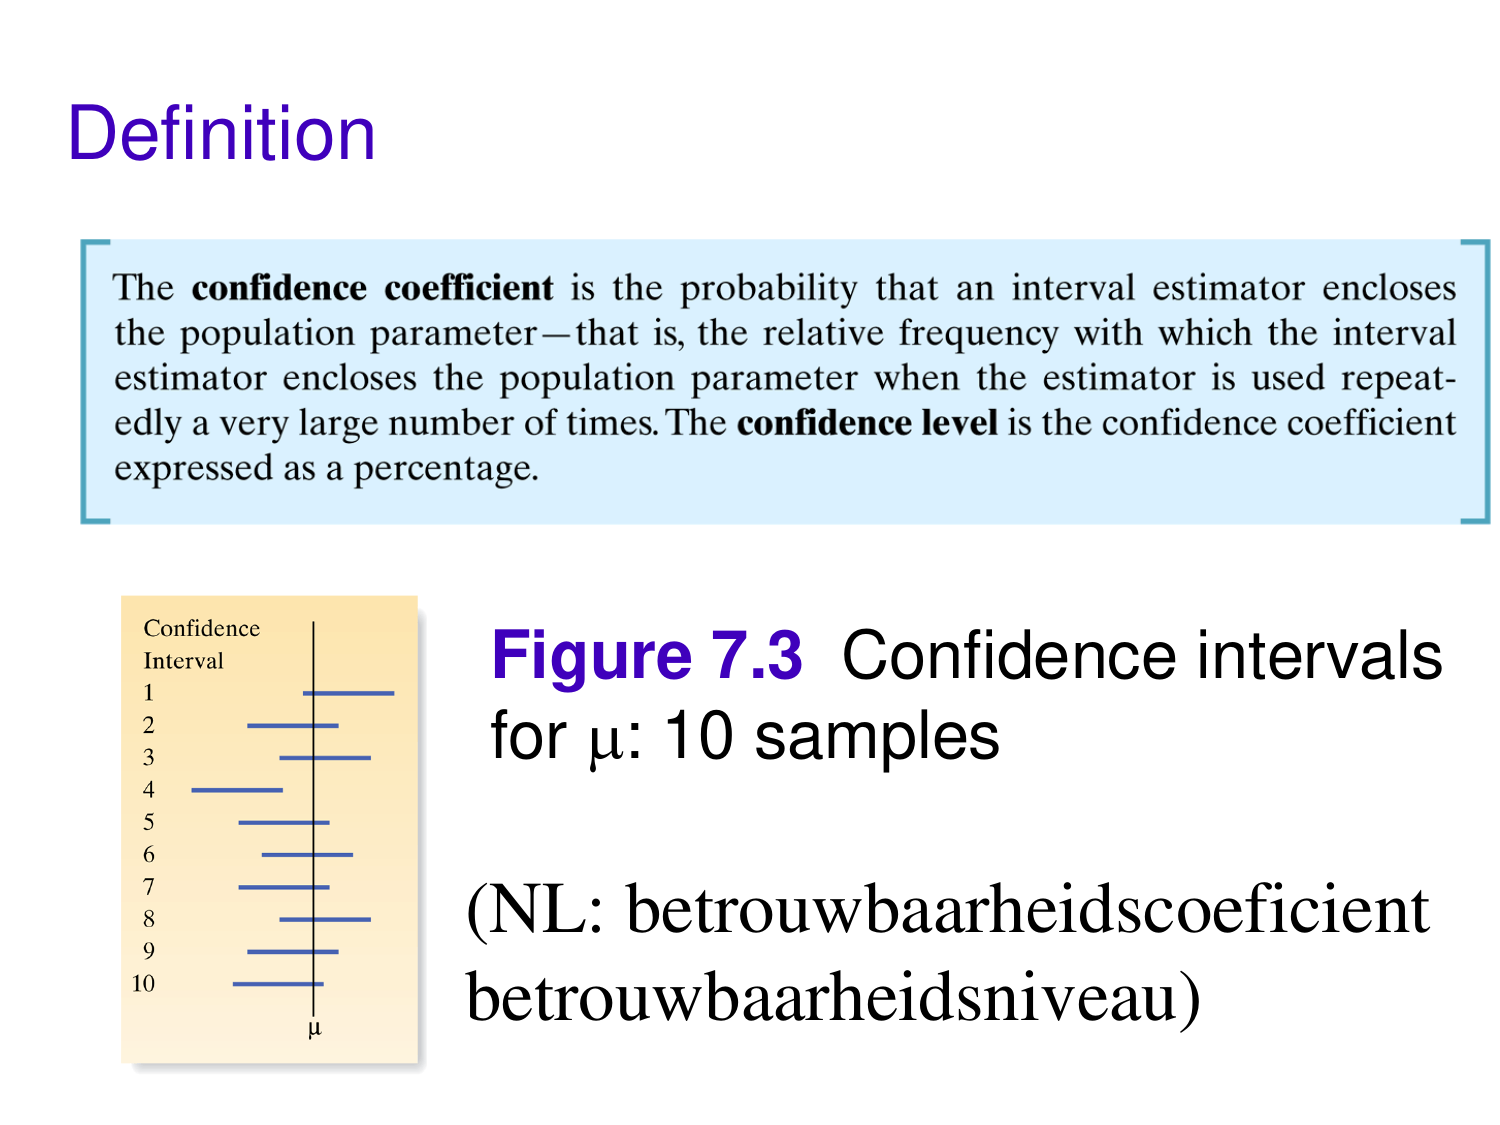
\includegraphics[width=0.72\textwidth]{assets/ch7-betrouwbaarheidsinterval-concept.png}
  \caption{Betrouwbaarheidsintervallen voor 10 verschillende steekproeven: gemiddeld 95\% van de intervallen bevatten $\mu$.}
\end{figure}

\begin{conceptbox}[Juiste interpretatie van een 95\%-CI]
\textbf{Correct:} ``Als we dit experiment heel vaak herhalen, zal 95\% van de zo berekende intervallen de werkelijke $\mu$ bevatten.''

\textbf{Fout:} ``Er is 95\% kans dat $\mu$ in dit specifieke interval ligt.'' ($\mu$ is een vaste waarde, niet stochastisch!)

Eenmaal berekend bevat een specifiek interval $\mu$ of niet -- je weet alleen niet welke van de twee het is.
\end{conceptbox}

\begin{figure}[h!]
  \centering
  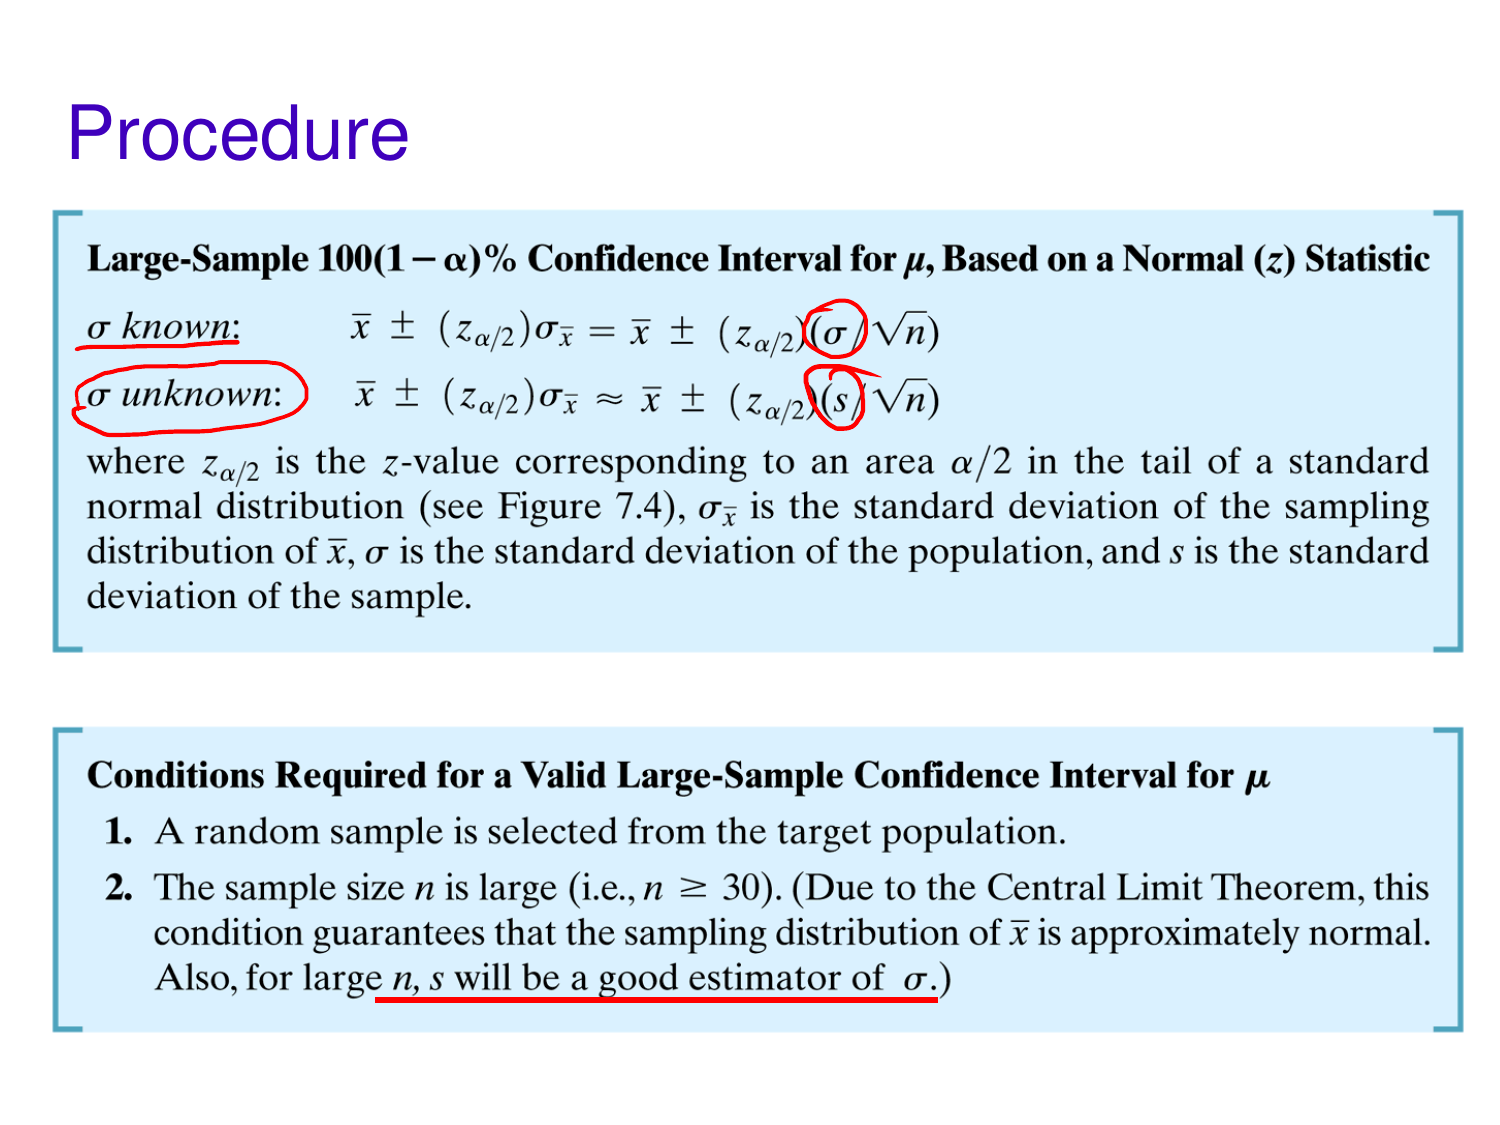
\includegraphics[width=0.72\textwidth]{assets/ch7-procedure-ci-z.png}
  \caption{Stappenplan voor het berekenen van een CI voor $\mu$ bij grote steekproeven (uit de slides).}
\end{figure}


\begin{pyblock}
import numpy as np
from scipy import stats as sts

n, xbar, s = 100, 5.2, 1.3
alpha = 0.05

# Methode 1: handmatig
z = sts.norm.ppf(1 - alpha/2)     # 1.96 voor 95%
marge = z * s / np.sqrt(n)
print(f"95% CI: ({xbar-marge:.3f}, {xbar+marge:.3f})")

# Bekende z-waarden: alpha=0.05 -> z=1.645 (eenzijdig) of 1.96 (tweezijdig)
#                   alpha=0.01 -> z=2.326 (eenzijdig) of 2.576 (tweezijdig)
\end{pyblock}
\subsection{7.3 -- CI voor $\mu$ met t-statistiek (kleine steekproef, $n < 30$)}

Voor kleine steekproeven ($n < 30$) werkt de z-aanpak niet goed meer: we schatten $\sigma$ met $s$, maar bij kleine steekproeven is $s$ zelf vrij onnauwkeurig. Dit voegt extra onzekerheid toe die de t-verdeling opvangt.

\begin{conceptbox}[De t-verdeling]
De \textbf{t-verdeling} lijkt op de standaard normale verdeling, maar heeft \emph{dikkere staarten} -- ze houdt rekening met de extra onzekerheid door $s$ te gebruiken in plaats van $\sigma$.

Kenmerken:
\begin{itemize}
  \item Symmetrisch en klokvormig rond 0, net als $z$.
  \item Heeft \textbf{vrijheidsgraden} (degrees of freedom): $\text{df} = n - 1$.
  \item Hoe kleiner $n$ (en dus $\text{df}$), hoe dikker de staarten.
  \item Voor grote $n$ ($> 100$) benadert de t-verdeling de standaard normale verdeling.
\end{itemize}
\end{conceptbox}

\begin{figure}[h!]
  \centering
  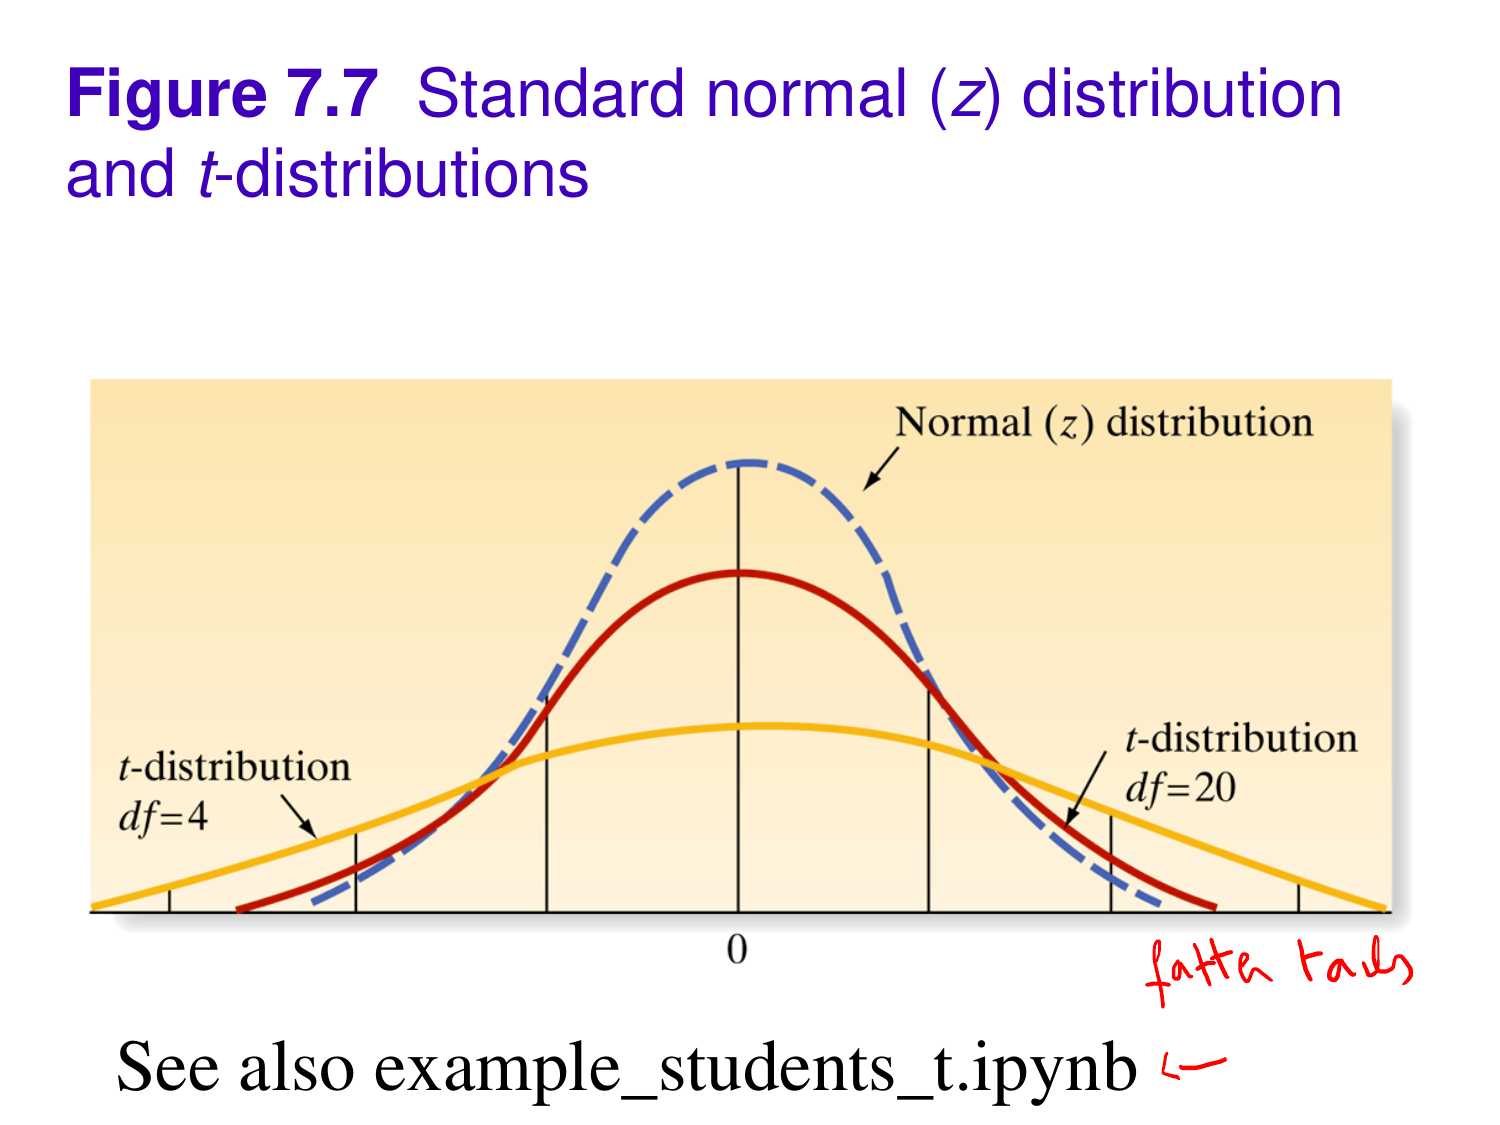
\includegraphics[width=0.68\textwidth]{assets/ch7-t-vs-z-verdeling.png}
  \caption{t-verdeling vs.\ standaard normale verdeling: de t heeft dikkere staarten voor kleine $n$.}
\end{figure}

\frm{t-statistiek}{t = \frac{\bar{x} - \mu}{s/\sqrt{n}}}{%
  Zelfde structuur als de z-score, maar met $s$ in plaats van $\sigma$. Heeft $n-1$ vrijheidsgraden (df).}

\frm{Betrouwbaarheidsinterval voor $\mu$ (kleine steekproef)}{\bar{x} \pm t_{\alpha/2,\, n-1} \cdot \frac{s}{\sqrt{n}}}{%
  $t_{\alpha/2,\,n-1}$ = t-waarde met $\text{df} = n-1$ vrijheidsgraden en oppervlak $\alpha/2$ in elke staart.\\
  \textbf{Voorwaarde:} de populatie moet (bij benadering) normaal verdeeld zijn!\\
  \textit{Controleer dit via histogram of normal probability plot.}}

\begin{figure}[h!]
  \centering
  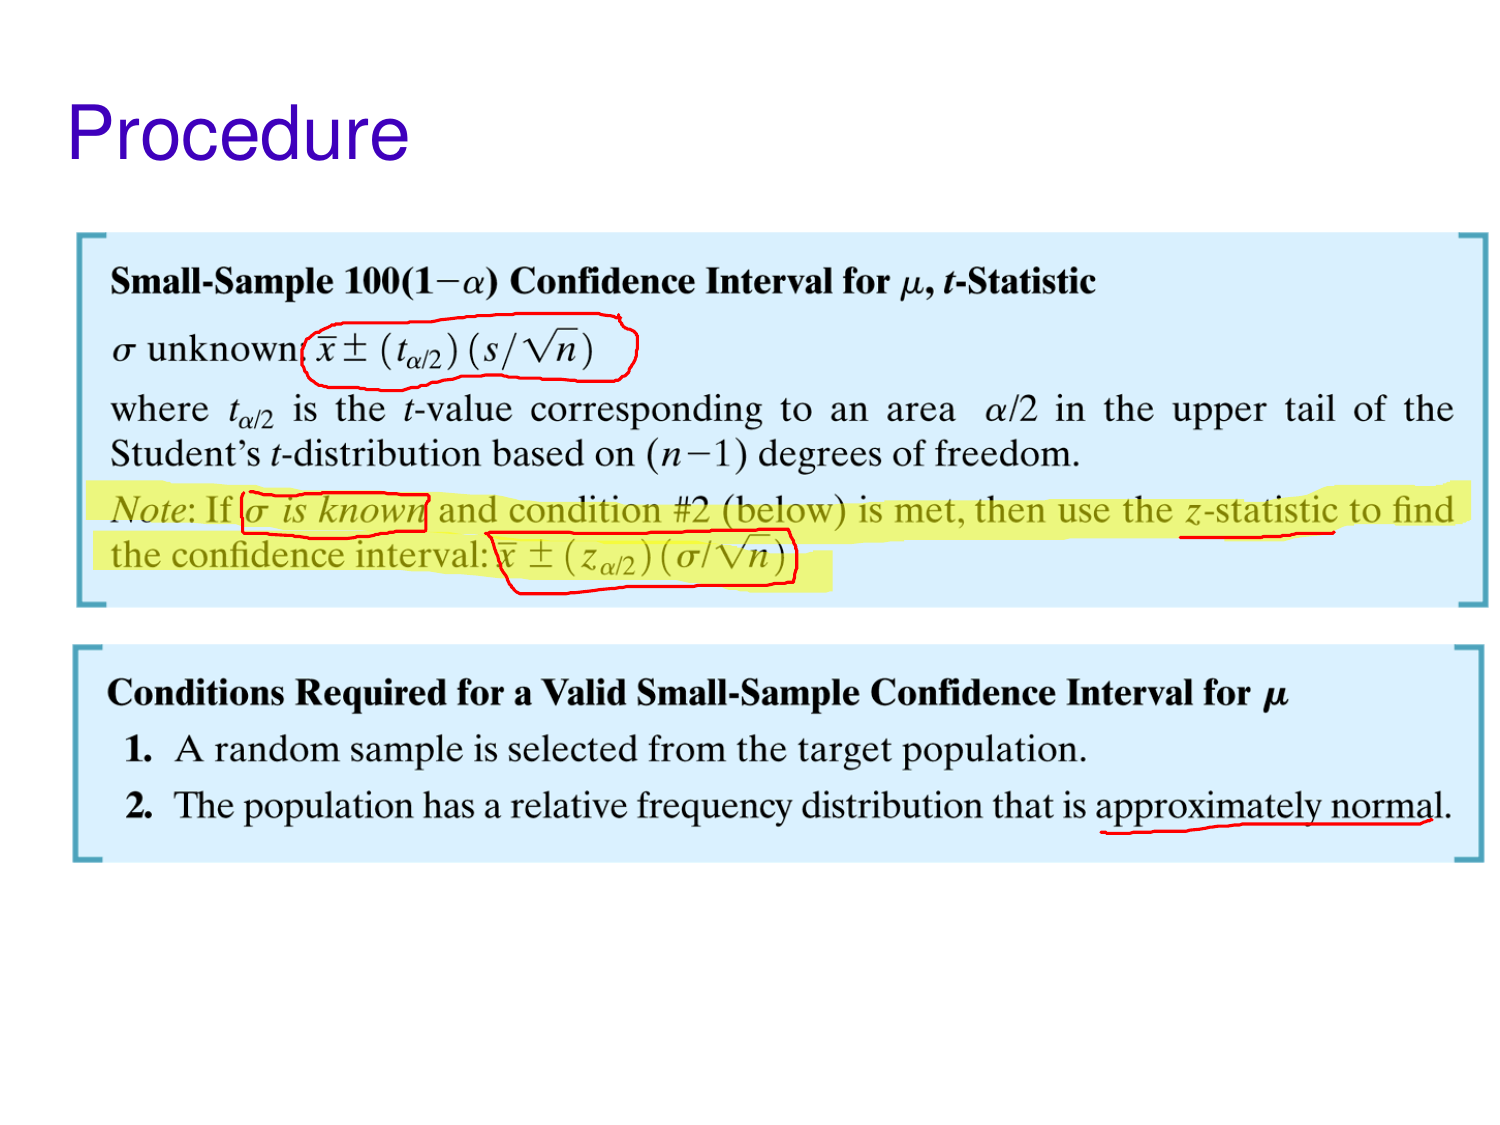
\includegraphics[width=0.68\textwidth]{assets/ch7-procedure-ci-t.png}
  \caption{Stappenplan voor CI voor $\mu$ bij kleine steekproeven (t-statistiek).}
\end{figure}

\begin{examenbox}
\textbf{Kies z of t?}
\begin{itemize}
  \item $n > 30$ en $\sigma$ gekend: gebruik $z$ met $\sigma$.
  \item $n > 30$ en $\sigma$ onbekend: gebruik $z$ met $s$ als benadering (CLT geldt).
  \item $n < 30$ en populatie normaal verdeeld: gebruik $t$ met $s$ en $\text{df} = n-1$.
  \item $n < 30$ en populatie \emph{niet} normaal: geen van beide technieken werkt -- overweeg niet-parametrische methodes.
\end{itemize}
\end{examenbox}


\begin{pyblock}
import numpy as np
from scipy import stats as sts

n, xbar, s = 15, 5.2, 1.3
alpha = 0.05

t = sts.t.ppf(1 - alpha/2, df=n-1)  # t-kritieke waarde
marge = t * s / np.sqrt(n)
print(f"95% CI: ({xbar-marge:.3f}, {xbar+marge:.3f})")

# Of met ruwe data:
# CI = sts.t.interval(1-alpha, df=n-1, loc=xbar, scale=s/np.sqrt(n))
\end{pyblock}
\subsection{7.4 -- CI voor een populatiefractie \texorpdfstring{$p$}{p} (grote steekproef)}

Soms wil je niet het gemiddelde schatten, maar een \emph{proportie} -- bv.\ het percentage klanten dat tevreden is, of de fractie defecte producten.

\begin{conceptbox}[Puntschatting van $p$]
De \textbf{steekproeffractie} $\hat{p}$ (schatting van de populatiefractie $p$) is:
\[\hat{p} = \frac{x}{n}\]
waarbij $x$ = aantal ``successen'' (bv.\ tevreden klanten) en $n$ = steekproefgrootte.

Voor grote steekproeven ($np \geq 15$ én $nq \geq 15$) geldt via de CLT:
\[\hat{p} \;\dot{\sim}\; \mathcal{N}\!\left(p,\, \frac{pq}{n}\right)\]
\end{conceptbox}

\frm{Betrouwbaarheidsinterval voor $p$ (grote steekproef)}{\hat{p} \pm z_{\alpha/2}\sqrt{\frac{\hat{p}\,\hat{q}}{n}}}{%
  met $\hat{q} = 1 - \hat{p}$.\\
  \textbf{Geldigheidsvoorwaarde:} $n\hat{p} \geq 15$ én $n\hat{q} \geq 15$.}

\begin{figure}[h!]
  \centering
  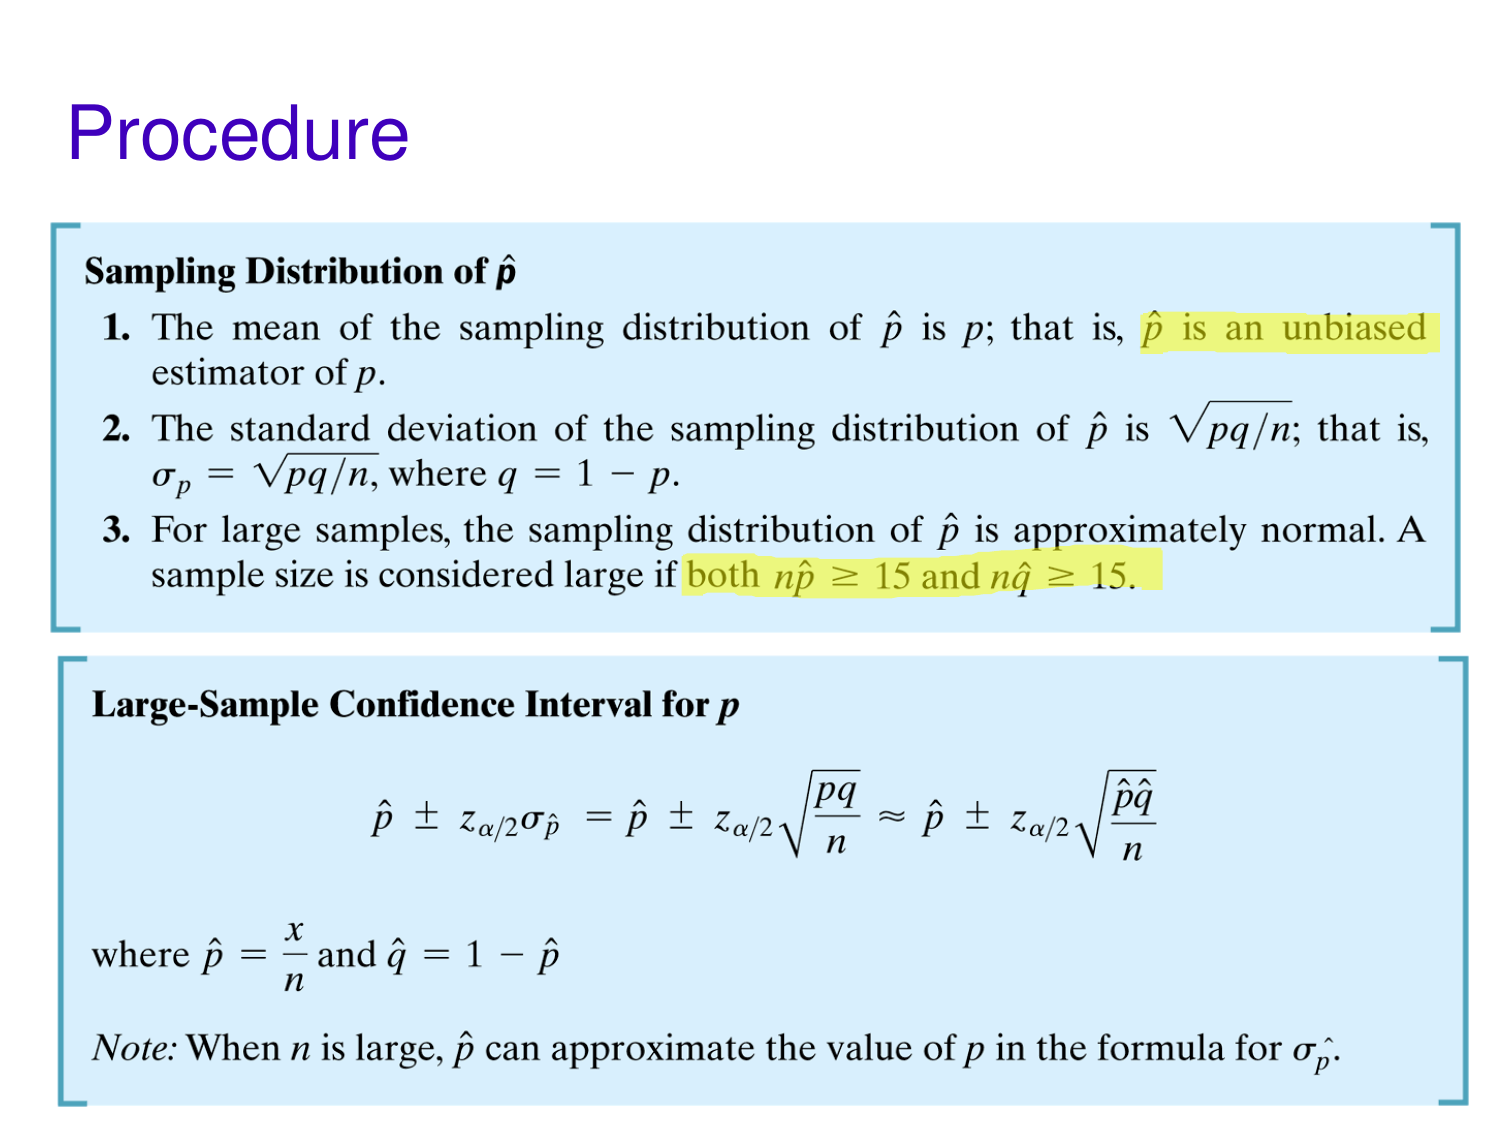
\includegraphics[width=0.68\textwidth]{assets/ch7-procedure-ci-proportie.png}
  \caption{Stappenplan voor CI voor populatiefractie $p$ (grote steekproef).}
\end{figure}

\begin{conceptbox}[Wilson's aanpassing voor kleine steekproeven of extreme $p$]
Als $n$ klein is, of $p$ dicht bij 0 of 1 ligt, werkt het grote-steekproefinterval slecht (je kan zelfs negatieve kansen krijgen). Wilson's aanpassing voegt kunstmatig 2 successen en 2 mislukkingen toe:
\[\tilde{p} = \frac{x+2}{n+4}, \qquad \tilde{n} = n + 4\]
en berekent het CI als: $\tilde{p} \pm z_{\alpha/2}\sqrt{\dfrac{\tilde{p}(1-\tilde{p})}{\tilde{n}}}$.
\end{conceptbox}


\begin{pyblock}
import numpy as np
from scipy import stats as sts

n, x = 200, 40                     # 40 successen in 200 pogingen
phat = x / n                       # = 0.20
alpha = 0.05

z = sts.norm.ppf(1 - alpha/2)
marge = z * np.sqrt(phat*(1-phat)/n)
print(f"95% CI: ({phat-marge:.4f}, {phat+marge:.4f})")

# Steekproefomvang berekenen (als p onbekend, gebruik phat=0.5):
SE = 0.03
n_nodig = int(np.ceil((z/SE)**2 * phat*(1-phat)))
print(f"Benodigde n: {n_nodig}")
\end{pyblock}
\subsection{7.5 -- Steekproefomvang bepalen}

Soms wil je van tevoren vastleggen hoe nauwkeurig je schatting moet zijn. Dan bereken je de benodigde steekproefgrootte $n$.

\begin{conceptbox}[De sampling error (SE)]
De \textbf{sampling error} (steekproeffout) is de \emph{halve breedte} van het betrouwbaarheidsinterval:
\[\text{SE} = z_{\alpha/2} \cdot \frac{\sigma}{\sqrt{n}}\]
Je kiest hoe groot de fout maximaal mag zijn, en berekent dan hoe groot $n$ moet zijn.
\end{conceptbox}

\frm{Benodigde steekproefomvang voor $\mu$}{n = \left(\frac{z_{\alpha/2} \cdot \sigma}{\text{SE}}\right)^2}{%
  \textbf{Afronden:} altijd \emph{naar boven} afronden (je wil zeker genoeg data).\\
  Als $\sigma$ onbekend: schat $\sigma \approx R/4$ (met $R$ het verwachte bereik) of gebruik een pilotstudie.\\
  Als $n < 30$: zet $n = 30$.}

\begin{figure}[h!]
  \centering
  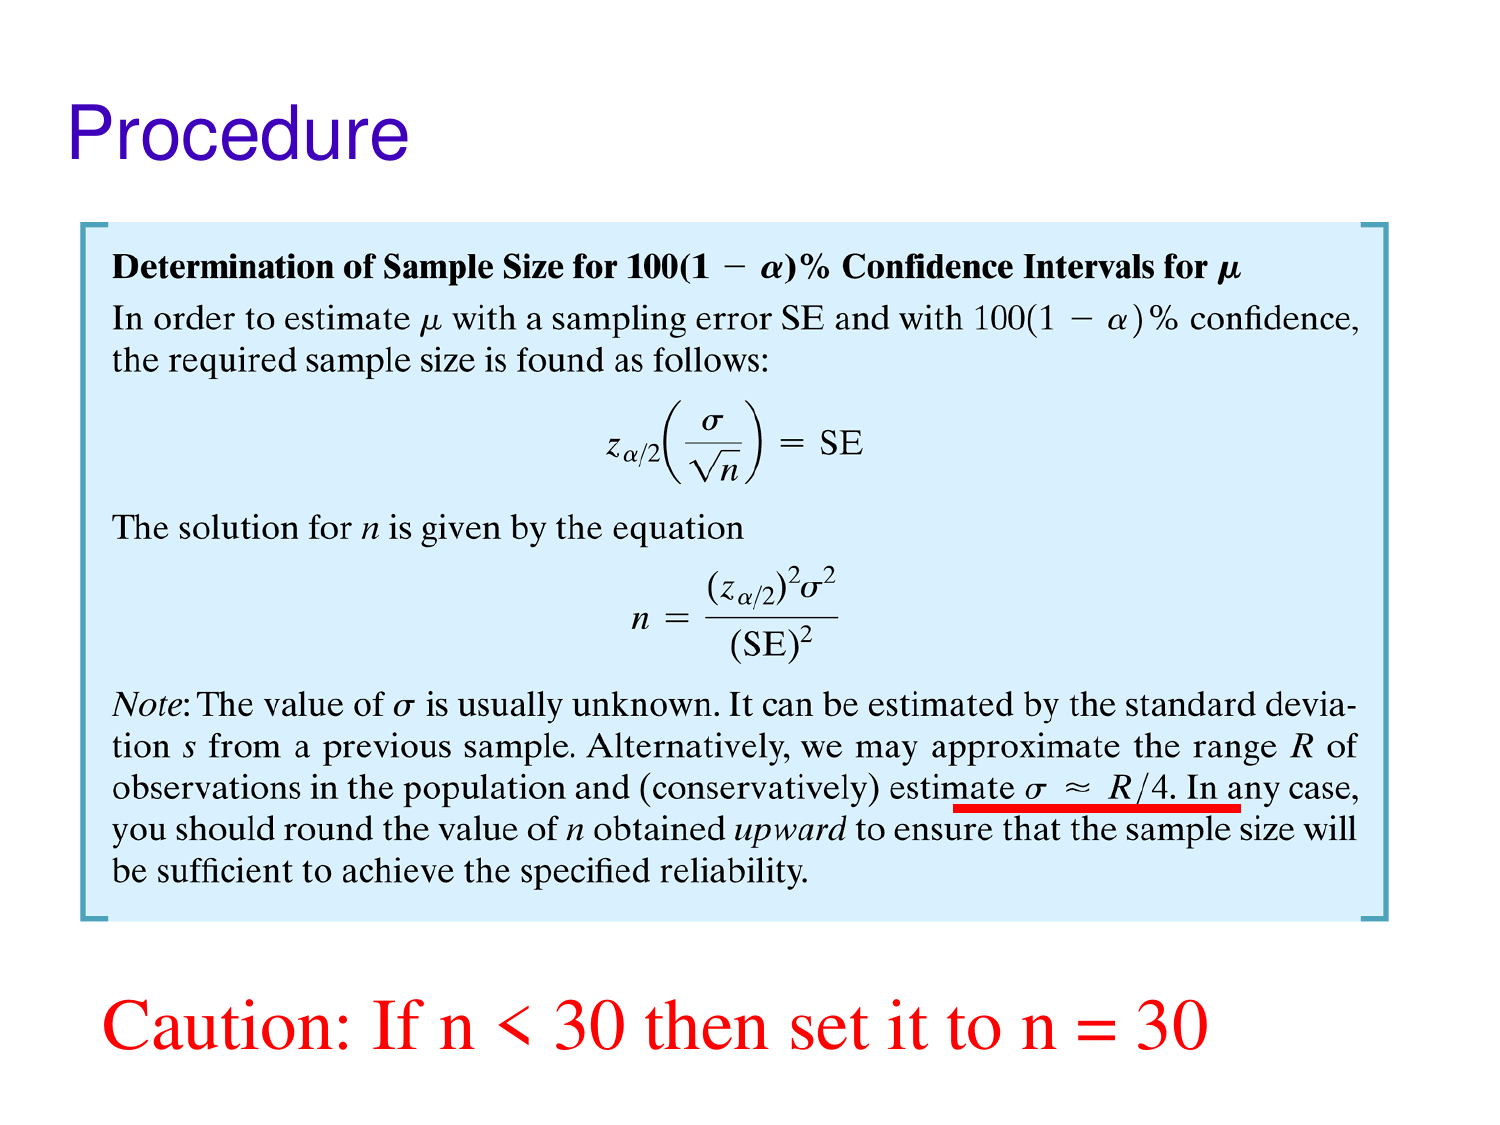
\includegraphics[width=0.72\textwidth]{assets/ch7-procedure-steekproefomvang-mu.png}
  \caption{Stappenplan voor het bepalen van de steekproefomvang voor $\mu$.}
\end{figure}

\frm{Benodigde steekproefomvang voor $p$}{n = \left(\frac{z_{\alpha/2}}{\text{SE}}\right)^2 \cdot \hat{p}\,\hat{q}}{%
  Als $p$ onbekend: gebruik de \emph{conservatieve} schatting $\hat{p} = 0{,}5$ (geeft maximale $n$).\\
  Als je een ruwe schatting van $p$ hebt, gebruik die -- je kan $n$ zo verlagen.}

\begin{figure}[h!]
  \centering
  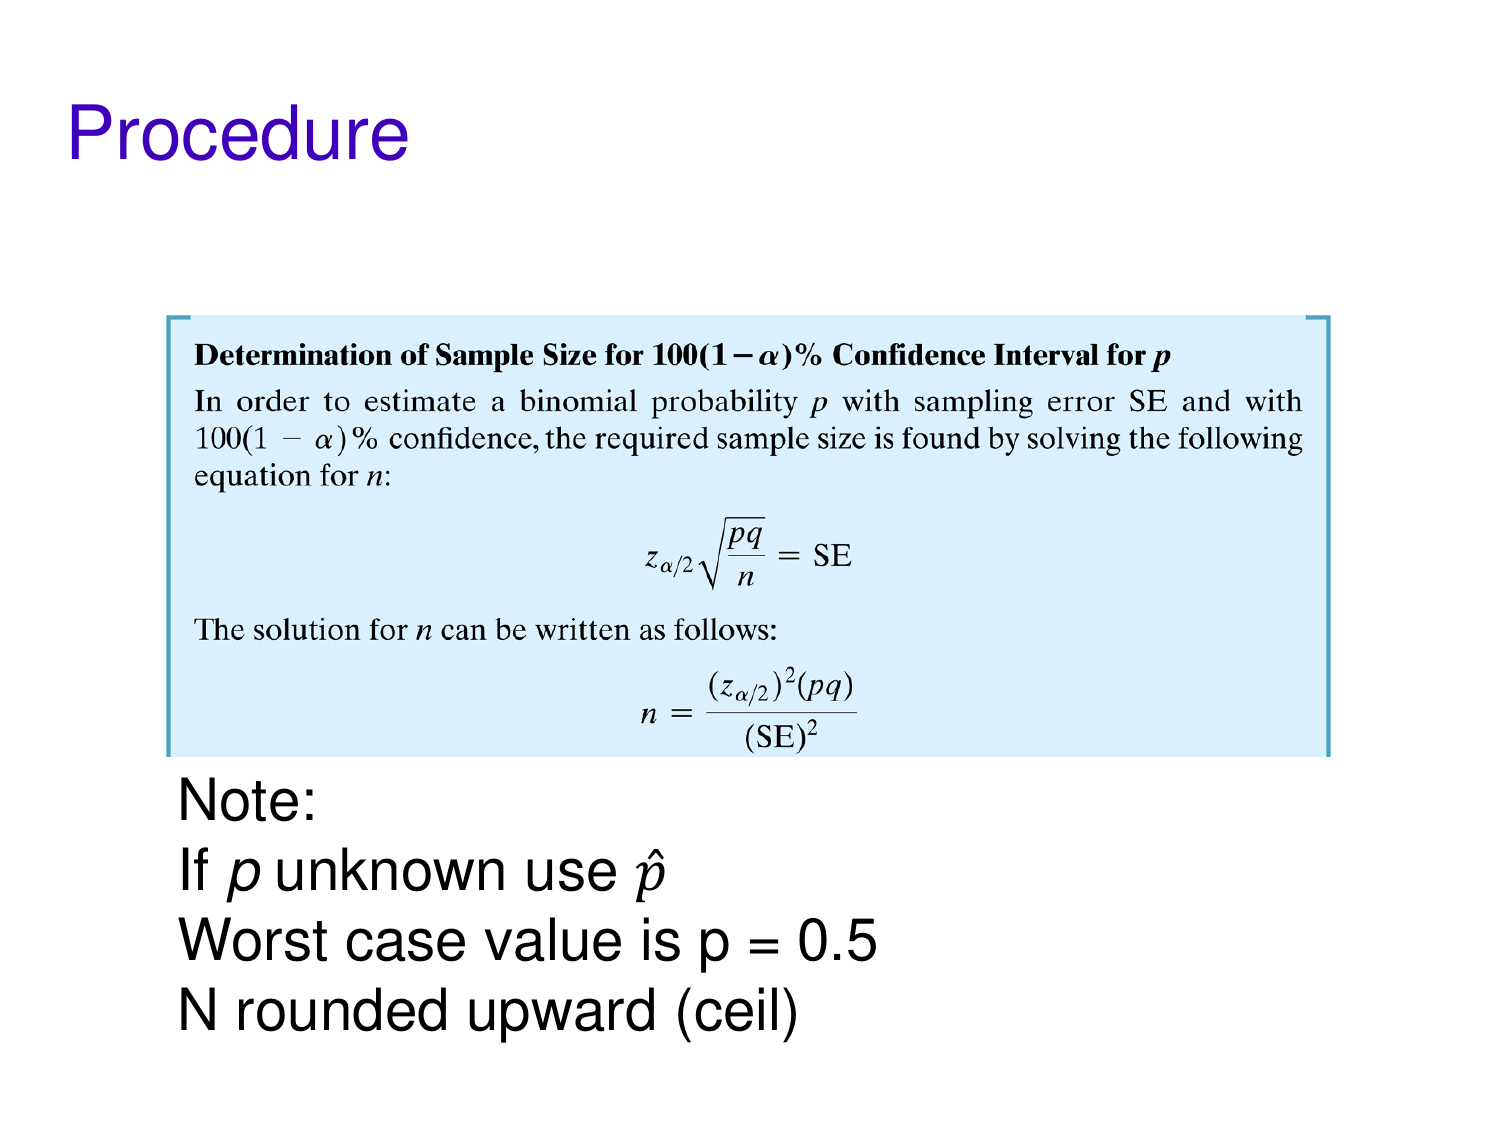
\includegraphics[width=0.72\textwidth]{assets/ch7-procedure-steekproefomvang-p.png}
  \caption{Stappenplan voor het bepalen van de steekproefomvang voor $p$.}
\end{figure}

\begin{figure}[h!]
  \centering
  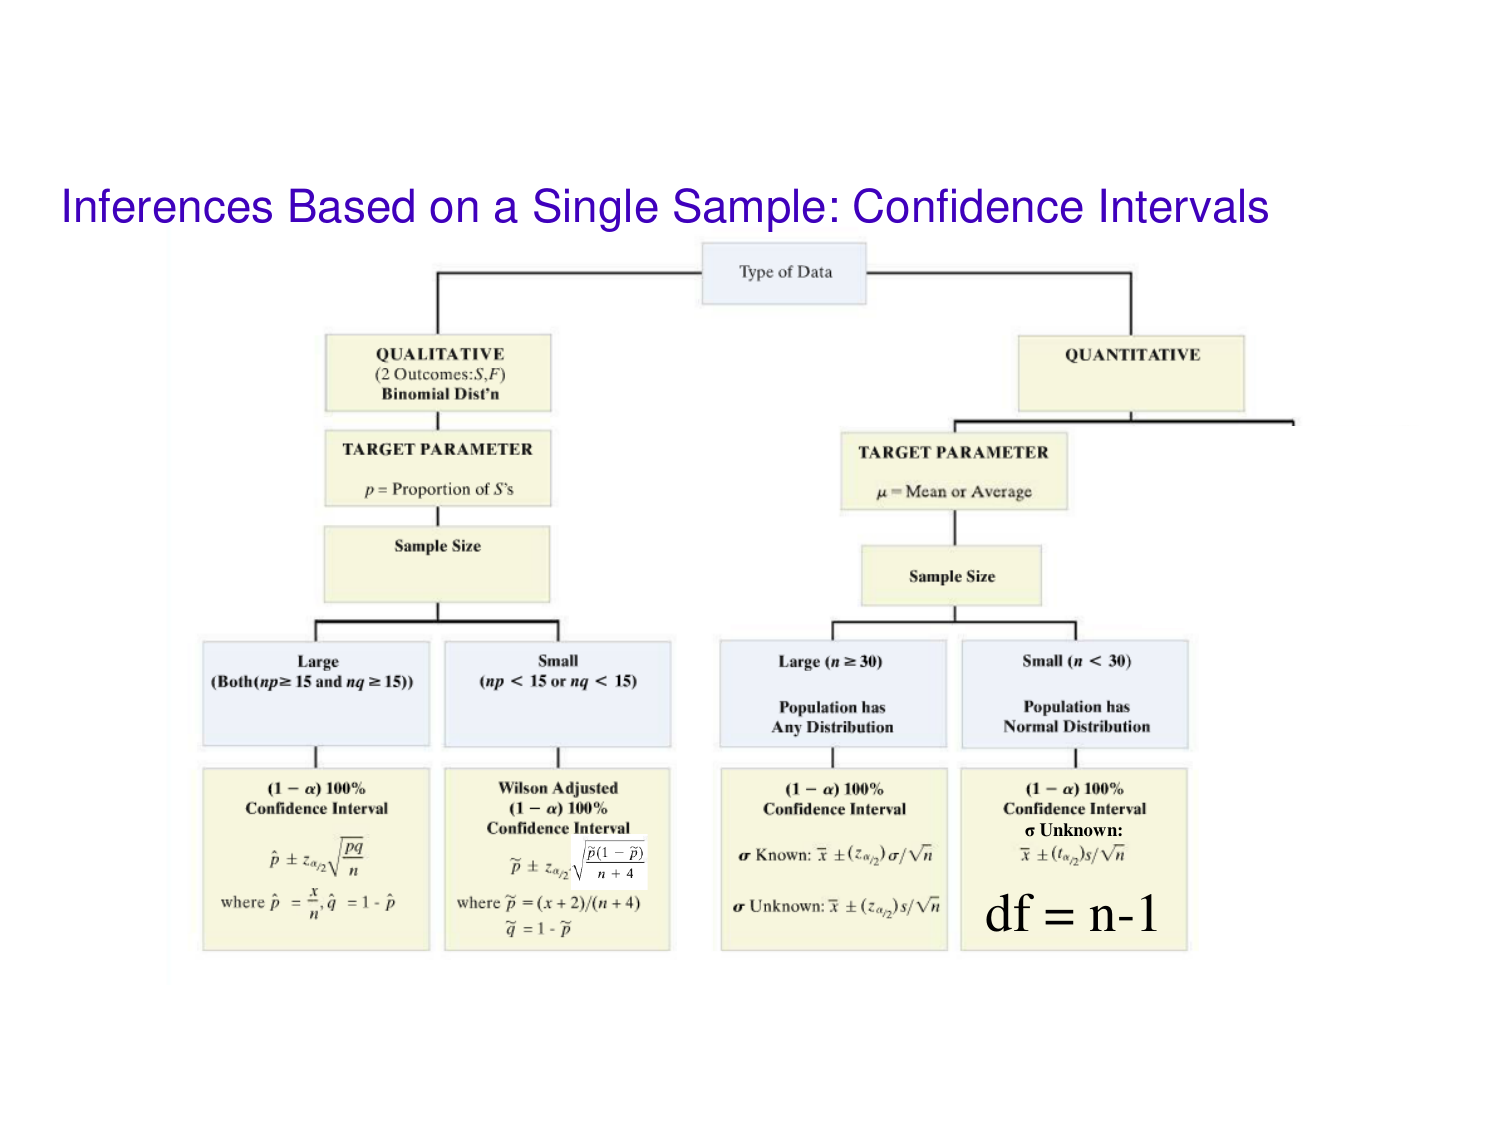
\includegraphics[width=0.72\textwidth]{assets/ch7-overzicht-formules.png}
  \caption{Overzicht van alle CI-formules uit Ch.\ 7 (uit de slides).}
\end{figure}

% =============================================================================
\section{Ch.\ 8 -- Toetsen van Hypothesen (één steekproef)}
% =============================================================================

\begin{conceptbox}{Wat is een hypothesetoets?}
Bij een \textbf{hypothesetoets} stel je een bewering op over een populatieparameter (bijv.\ $\mu = 2400$) en gebruik je steekproefdata om te beslissen of die bewering houdbaar is. Het is een formeel beslissingsproces met een vaste foutmarge.

\medskip
\textbf{Intuïtie:} Je stelt nooit vast dat iets \emph{zeker} waar is -- je toetst of de data \emph{voldoende bewijs} leveren om de nulhypothese te verwerpen.
\end{conceptbox}

\subsection{De elementen van een hypothesetoets}

\begin{theorieblok}{Hypothesen en toetsingsgrootheid}
\begin{itemize}
  \item \textbf{Nulhypothese} $H_0$: de bewering die je \emph{wil weerleggen} (altijd een gelijkheid, bijv.\ $\mu = \mu_0$).
  \item \textbf{Alternatieve hypothese} $H_a$: wat je wilt aantonen (eenzijdig of tweezijdig).
  \item \textbf{Toetsingsgrootheid} (\emph{test statistic}): een berekende waarde uit de steekproef (bijv.\ $z$ of $t$) die zegt hoe ver je steekproefgemiddelde van $\mu_0$ ligt.
  \item \textbf{Kritiek gebied} (\emph{rejection region}): het gebied van waarden waarvoor je $H_0$ verwerpt.
  \item \textbf{Significantieniveau} $\alpha$: de kans op een fout van de eerste soort (kans op onterecht verwerpen van $H_0$). Typisch $\alpha = 0{,}05$ of $0{,}01$.
\end{itemize}
\end{theorieblok}

\begin{figure}[h!]
  \centering
  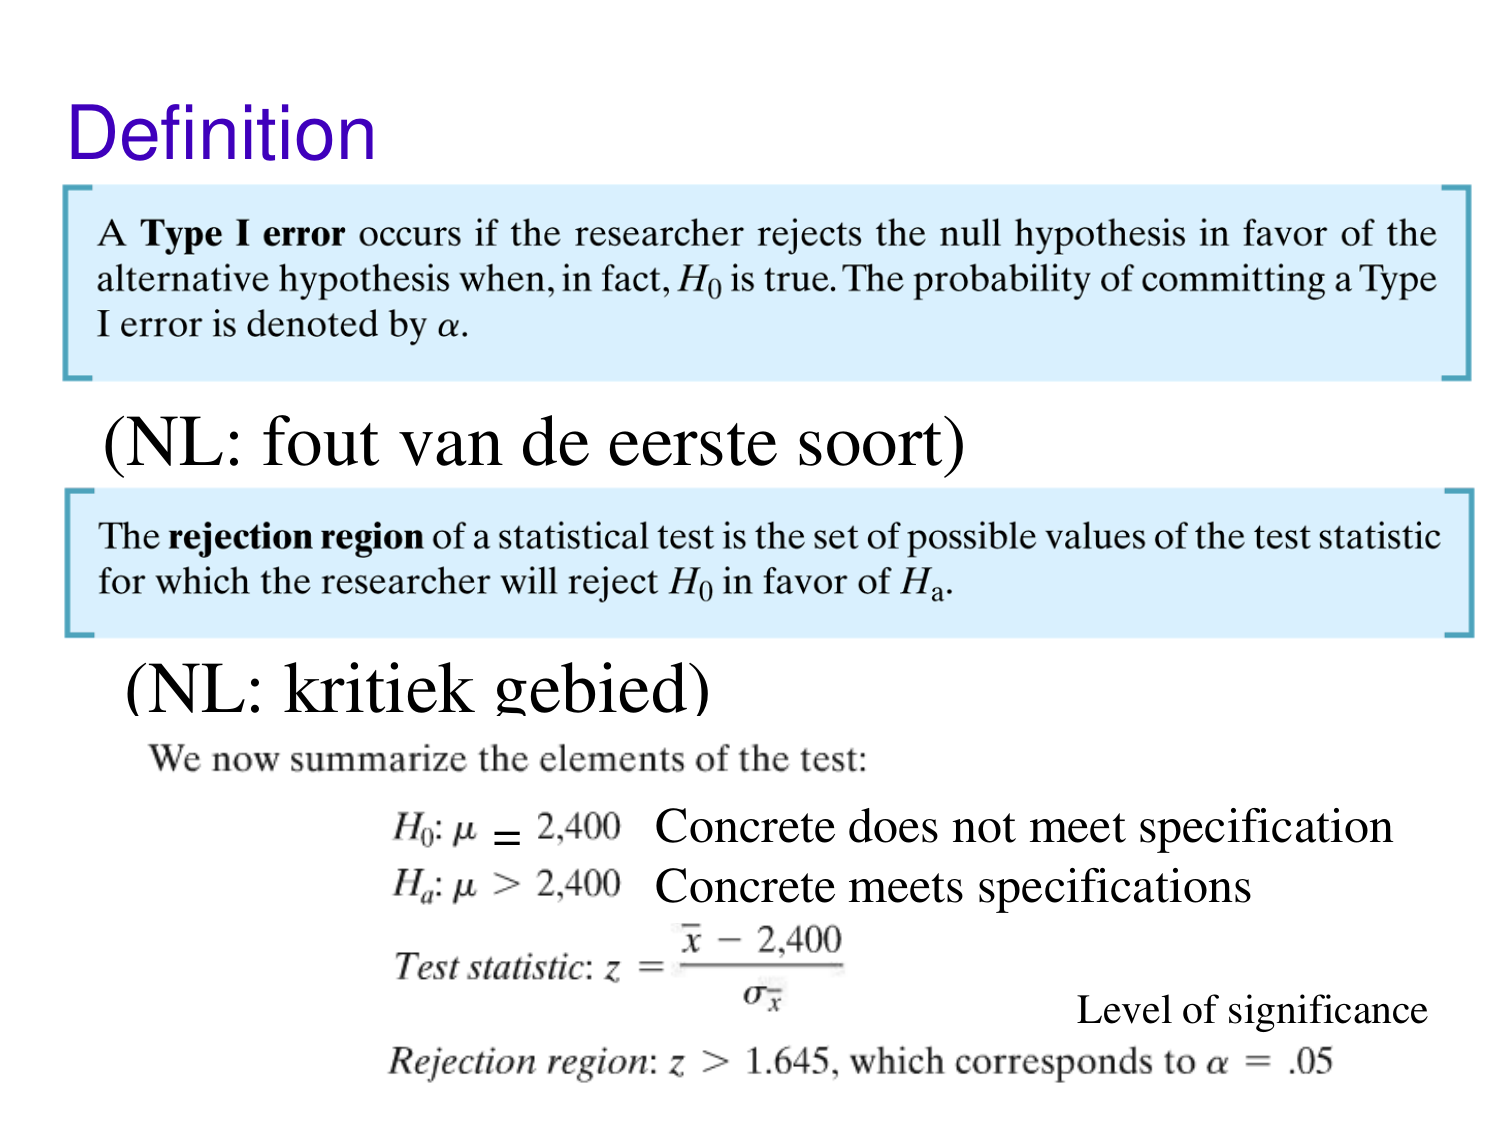
\includegraphics[width=0.75\textwidth]{assets/ch8-type1-type2-errors.png}
  \caption{Type I en Type II fouten: $\alpha$ = kans op vals positief (FP), $\beta$ = kans op vals negatief (FN).}
\end{figure}

\begin{conceptbox}{Type I en Type II fouten}
\begin{tabular}{lll}
  \hline
  & $H_0$ \textbf{is waar} & $H_0$ \textbf{is fout} \\
  \hline
  \textbf{Verwerp} $H_0$ & Type I fout ($\alpha$) & Correct (power $= 1-\beta$) \\
  \textbf{Verwerp niet} $H_0$ & Correct & Type II fout ($\beta$) \\
  \hline
\end{tabular}

\medskip
Als je $\alpha$ verlaagt, stijgt $\beta$ (en omgekeerd). De enige manier om beide tegelijk te verlagen is de steekproefgrootte $n$ verhogen.
\end{conceptbox}

\sym{alpha}{Significantieniveau (kans op Type I fout)}{--}
\sym{beta}{Kans op Type II fout}{--}

\subsection{Eenzijdige en tweezijdige toetsen}

\begin{theorieblok}{Formulering van $H_a$}
\[
  H_a: \mu > \mu_0 \quad \text{(rechtszijdig)} \qquad
  H_a: \mu < \mu_0 \quad \text{(linkszijdig)} \qquad
  H_a: \mu \neq \mu_0 \quad \text{(tweezijdig)}
\]
\begin{itemize}
  \item \textbf{Rechtszijdig}: kritiek gebied in de rechterstaart; verwerp als $z > z_\alpha$.
  \item \textbf{Linkszijdig}: kritiek gebied in de linkerstaart; verwerp als $z < -z_\alpha$.
  \item \textbf{Tweezijdig}: kritiek gebied in beide staarten; verwerp als $|z| > z_{\alpha/2}$.
\end{itemize}
\end{theorieblok}

\begin{figure}[h!]
  \centering
  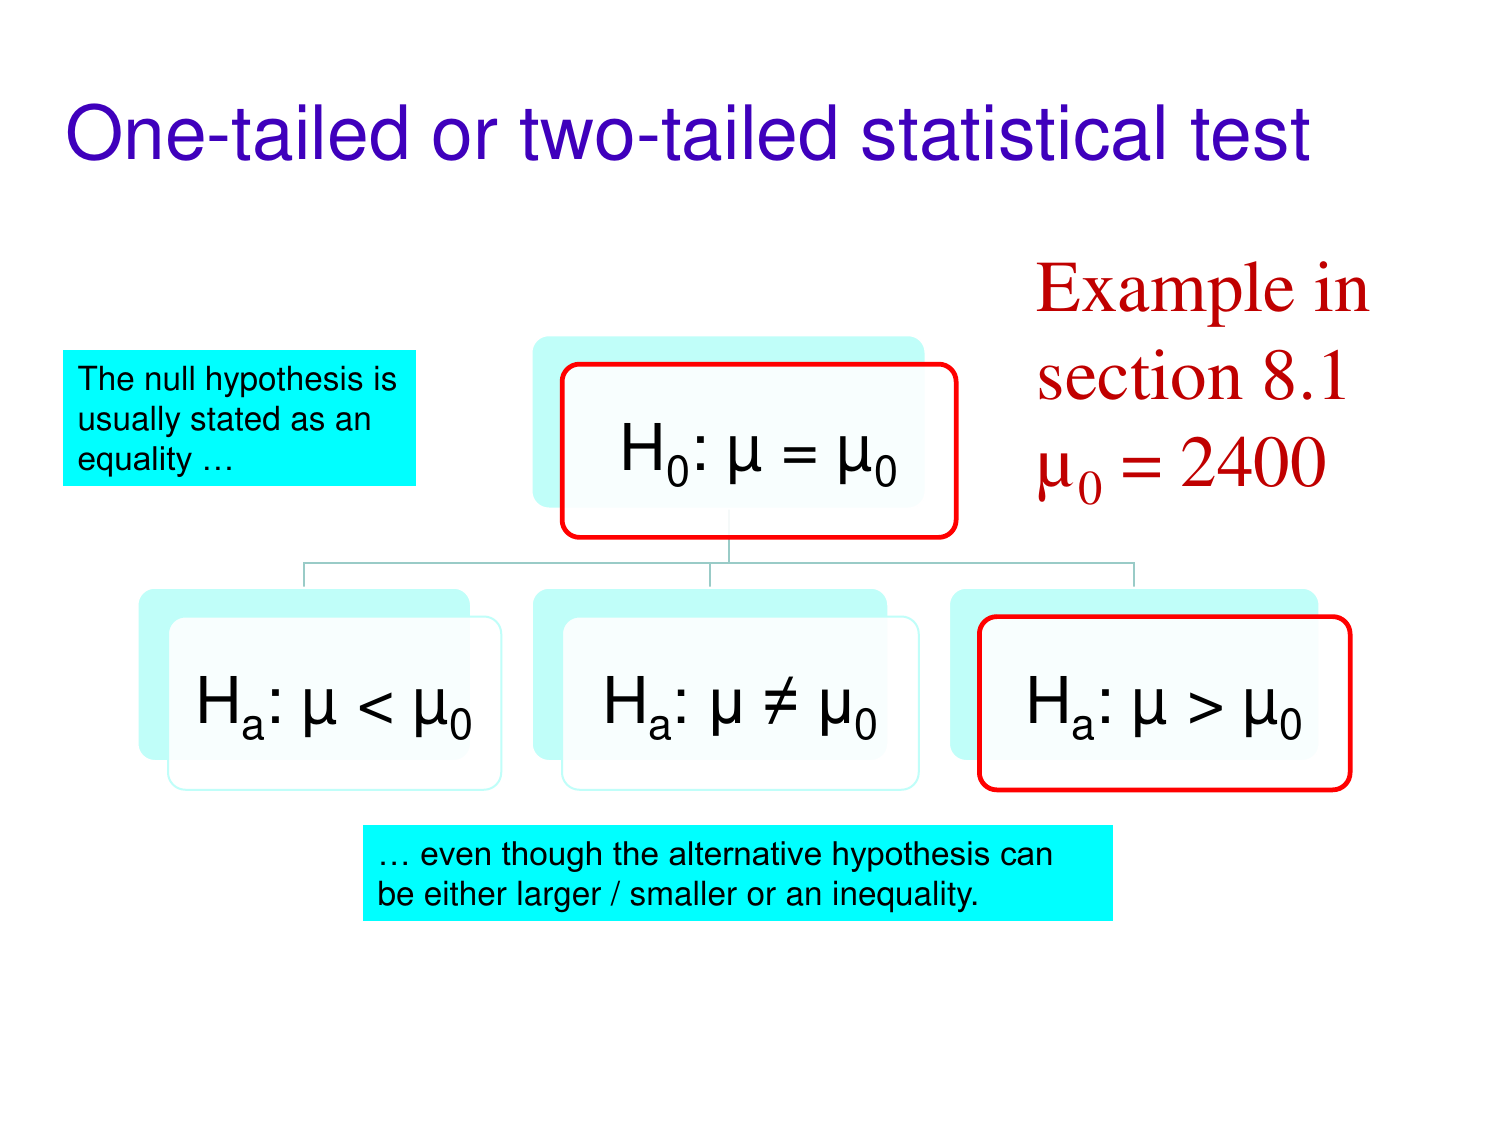
\includegraphics[width=0.78\textwidth]{assets/ch8-eenzijdig-tweezijdig.png}
  \caption{Kritieke gebieden voor eenzijdige en tweezijdige toetsen (uit de slides).}
\end{figure}

\subsection{Z-toets voor het populatiegemiddelde (grote steekproef)}

Gebruik als $n \geq 30$ of $\sigma$ bekend is.

\frm{Toetsingsgrootheid $z$ voor $\mu$}{z = \frac{\bar{x} - \mu_0}{\sigma / \sqrt{n}}}{%
  $\bar{x}$ = steekproefgemiddelde, $\mu_0$ = getoetste waarde onder $H_0$, $\sigma$ = populatiestandaardafwijking (of $s$ bij $n \geq 30$), $n$ = steekproefgrootte.
  Verwerp $H_0$ als $z$ in het kritieke gebied valt.}

\begin{figure}[h!]
  \centering
  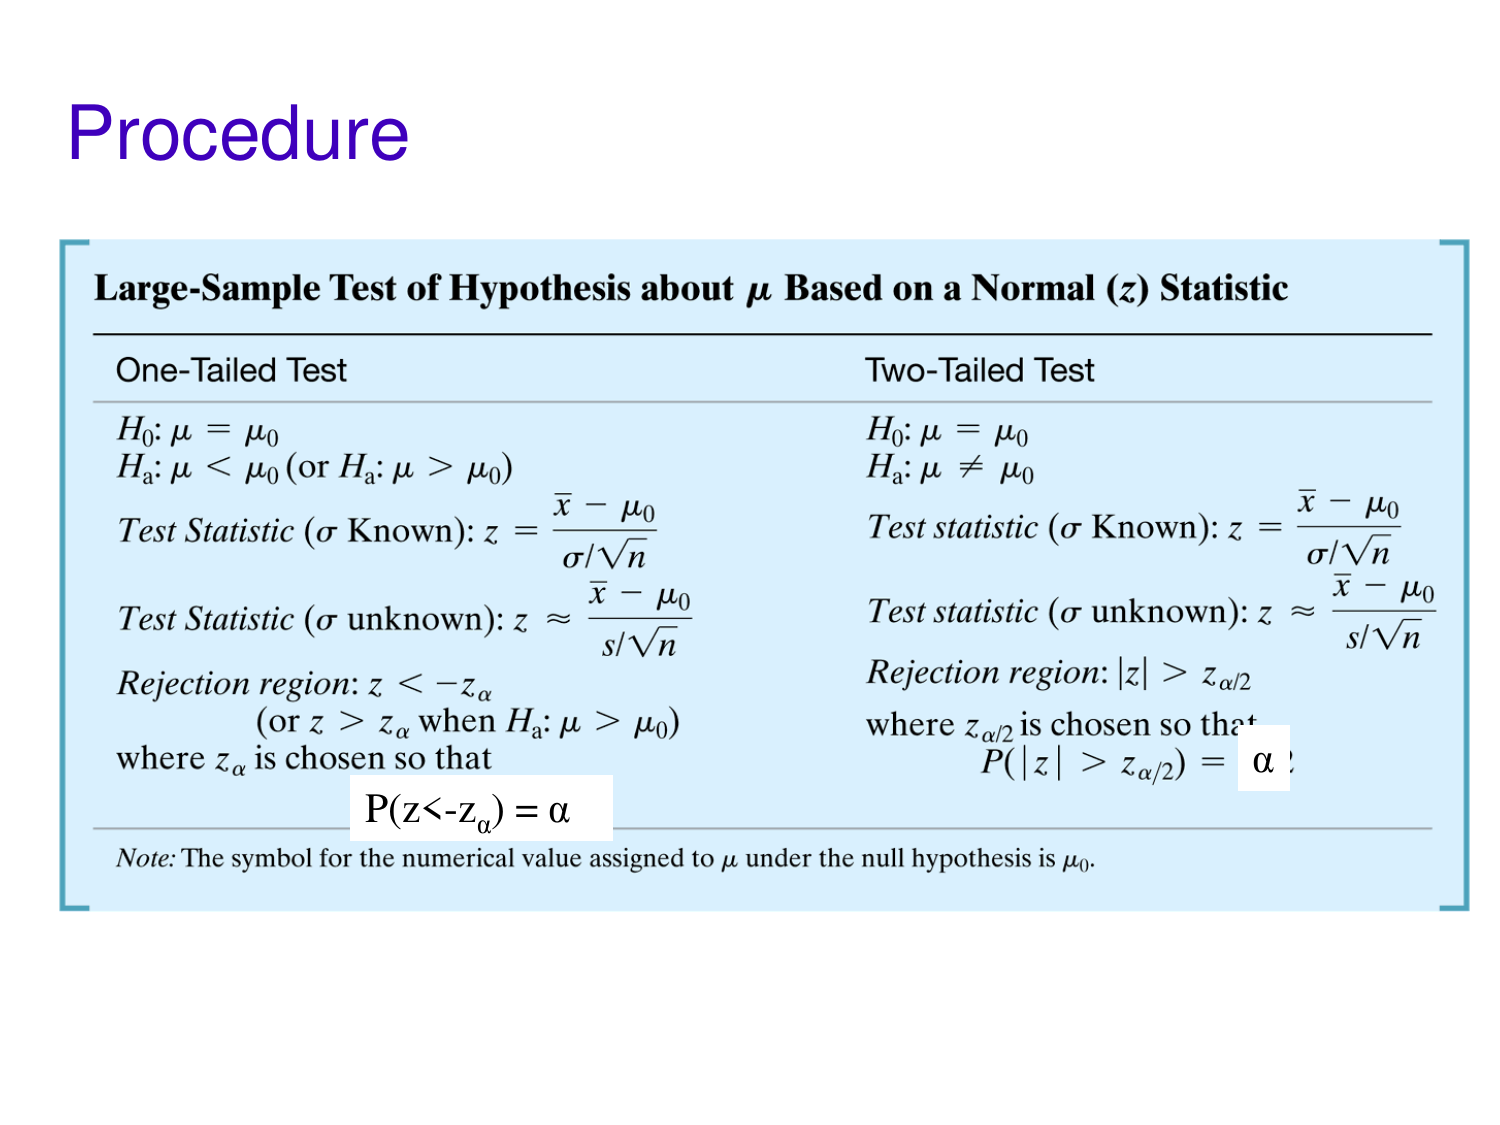
\includegraphics[width=0.78\textwidth]{assets/ch8-z-toets-procedure.png}
  \caption{Stappenplan voor de z-toets (grote steekproef).}
\end{figure}

\begin{examenbox}
\textbf{Stappenplan hypothesetoets:}
\begin{enumerate}
  \item Stel $H_0$ en $H_a$ op.
  \item Kies de toetsingsgrootheid.
  \item Bepaal het kritieke gebied (op basis van $\alpha$ en de richting van $H_a$).
  \item Controleer de aannames.
  \item Bereken de toetsingsgrootheid uit de steekproef.
  \item Trek een conclusie: verwerp of verwerp niet $H_0$.
\end{enumerate}
\end{examenbox}

\begin{figure}[h!]
  \centering
  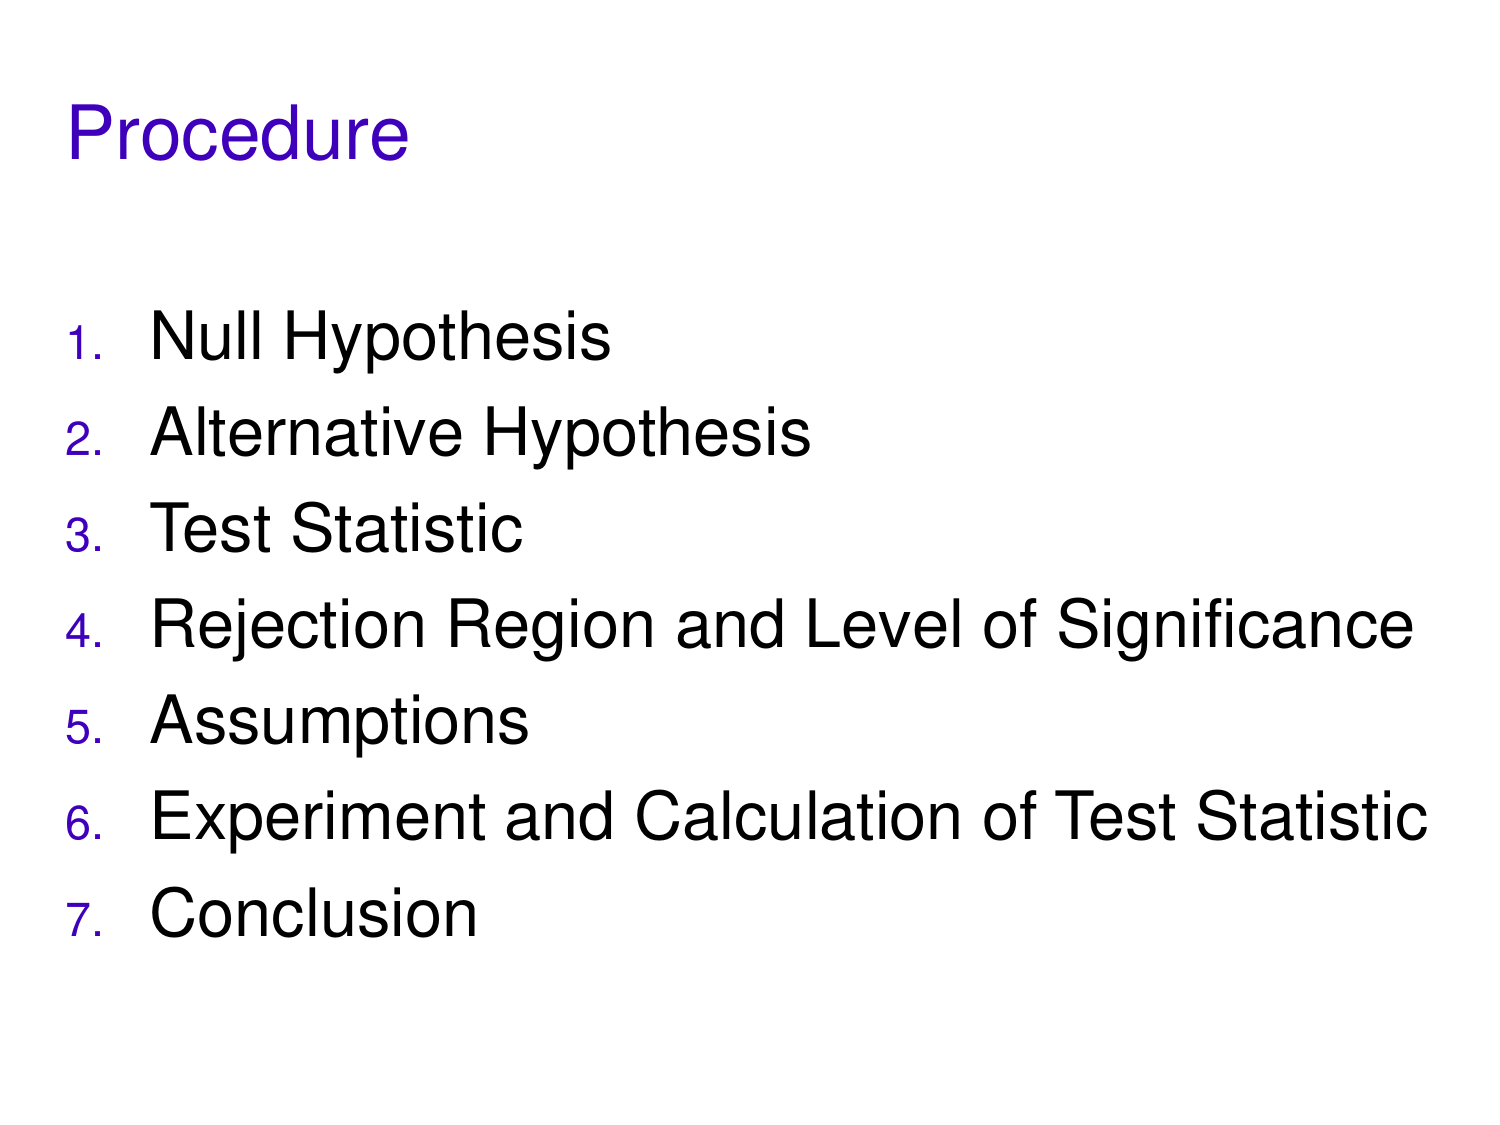
\includegraphics[width=0.78\textwidth]{assets/ch8-procedure-stappen.png}
  \caption{Visueel stappenplan uit de slides.}
\end{figure}


\begin{voorbeeld}[Voorbeeld: betonsterkte (rechtszijdige z-toets)]
Eis: $\mu > 2400$ kPa. Steekproef: $n=50$, $\bar{x}=2460$, $s=200$.

$H_0: \mu = 2400$, $H_a: \mu > 2400$, $\alpha = 0{,}05 \Rightarrow z_\alpha = 1{,}645$.
$$z = \frac{2460 - 2400}{200/\sqrt{50}} = \frac{60}{28{,}28} = 2{,}12$$
Beslissing: $2{,}12 > 1{,}645$ $\Rightarrow$ verwerp $H_0$. Beton voldoet.
\end{voorbeeld}

\begin{pyblock}
import numpy as np
from scipy import stats as sts

# Invoer
xbar, mu0, s, n = 2460, 2400, 200, 50
alpha = 0.05

# Toetsingsgrootheid
z = (xbar - mu0) / (s / np.sqrt(n))
print(f"z = {z:.3f}")             # 2.121

# p-waarden:
p_rechts  = sts.norm.sf(z)        # P(Z > z) -- rechtszijdig H_a: mu > mu0
p_links   = sts.norm.cdf(z)       # P(Z < z) -- linkszijdig H_a: mu < mu0
p_twee    = 2 * sts.norm.sf(abs(z))  # tweezijdig H_a: mu != mu0
print(f"p (rechts) = {p_rechts:.4f}")   # 0.0170

# Kritieke waarden:
z_rechts = sts.norm.ppf(1 - alpha)      # 1.645 (rechtszijdig)
z_twee   = sts.norm.ppf(1 - alpha/2)   # 1.960 (tweezijdig)
\end{pyblock}
\subsection{De p-waarde (overschrijdingskans)}

\begin{conceptbox}{Wat is de p-waarde?}
De \textbf{p-waarde} is de kans om, als $H_0$ waar is, een toetsingsgrootheid te observeren die \emph{minstens zo extreem} is als de berekende waarde. Hoe kleiner de p-waarde, hoe sterker het bewijs tegen $H_0$.

\medskip
\textbf{Beslissingsregel:} Als $p\text{-waarde} \leq \alpha$ $\Rightarrow$ verwerp $H_0$. Anders: onvoldoende bewijs.

\medskip
In Python: \texttt{1 - sts.norm.cdf(z)} (rechtszijdig), \texttt{sts.norm.cdf(z)} (linkszijdig), \texttt{2*(1 - sts.norm.cdf(|z|))} (tweezijdig).
\end{conceptbox}

\begin{figure}[h!]
  \centering
  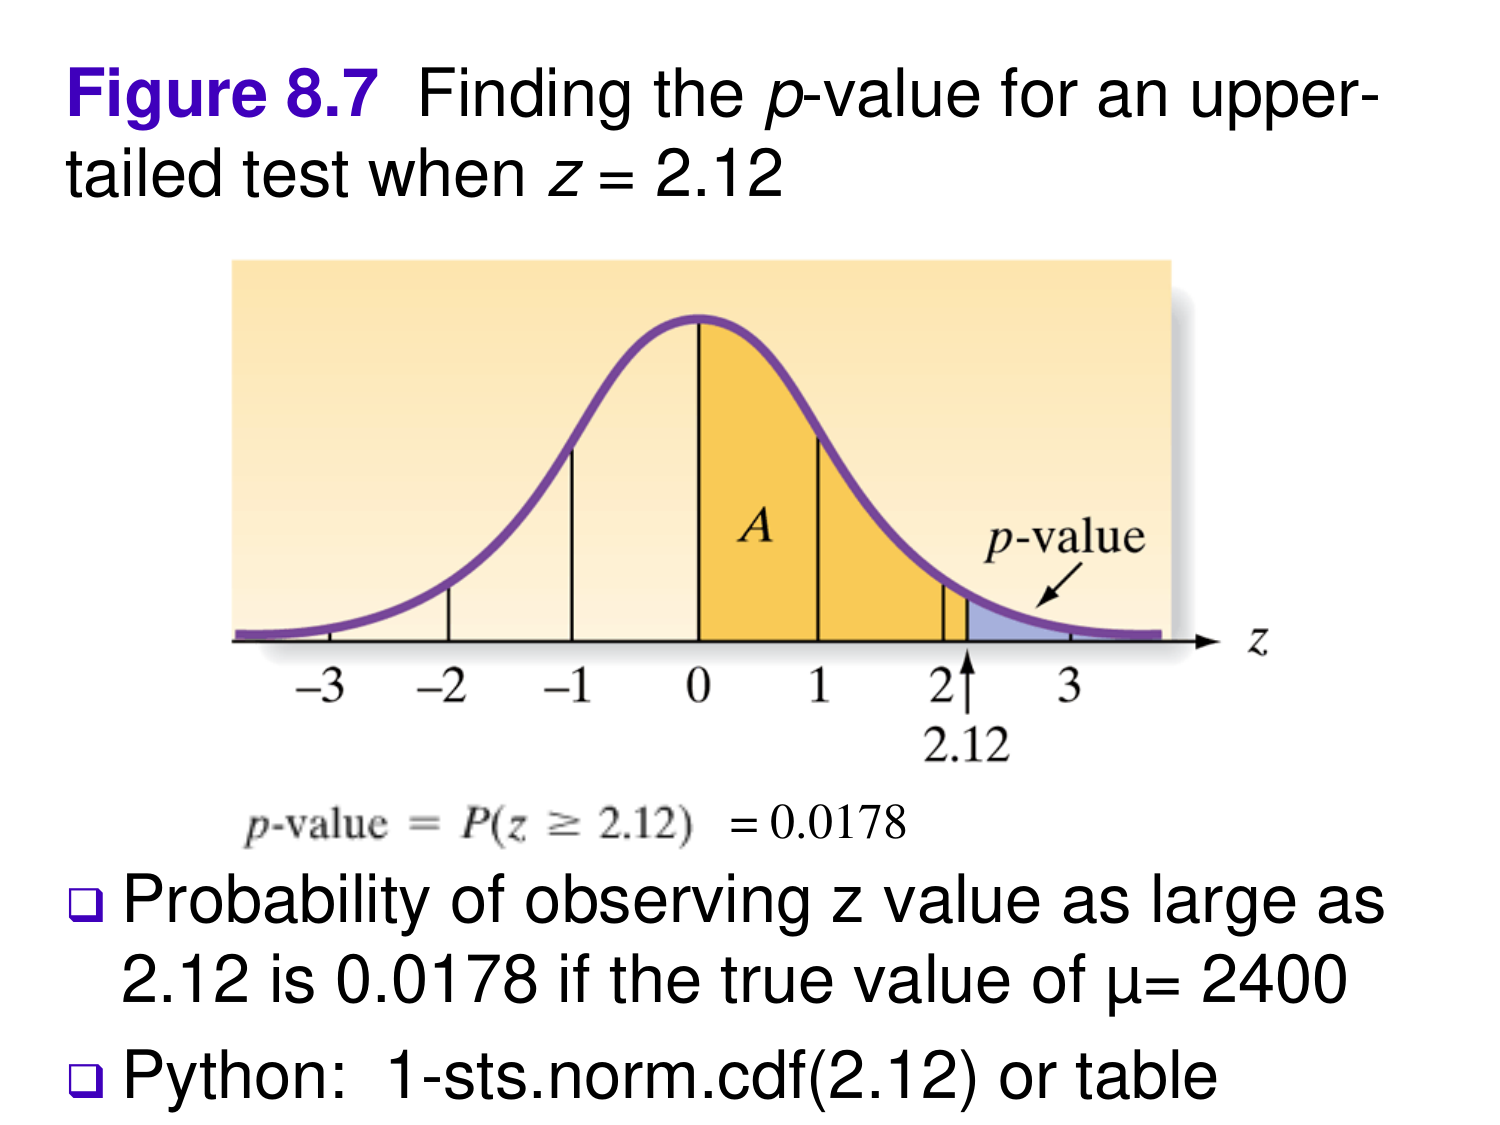
\includegraphics[width=0.75\textwidth]{assets/ch8-pwaarde-rechtszijdig.png}
  \caption{Grafische weergave van de p-waarde voor een rechtszijdige z-toets.}
\end{figure}

\frm{P-waarde rechtszijdige toets}{p = P(Z > z_{\text{berekend}}) = 1 - \Phi(z)}{%
  $\Phi(z)$ = cumulatieve standaard normaalverdeling. Tweezijdig: $p = 2\,P(Z > |z|)$.}


\begin{pyblock}
from scipy import stats as sts

# Als je z al berekend hebt:
z = 2.121
p_rechts   = sts.norm.sf(z)             # = 1 - norm.cdf(z)
p_links    = sts.norm.cdf(z)
p_tweezijdig = 2 * sts.norm.sf(abs(z))

# Als je t al berekend hebt (kleine steekproef, df=n-1):
t, df = -3.0, 9
p_tweezijdig = 2 * sts.t.cdf(-abs(t), df=df)

# Beslissing: p <= alpha => verwerp H_0
alpha = 0.05
print("Verwerp H_0" if p_rechts <= alpha else "Verwerp H_0 NIET")
\end{pyblock}
\subsection{T-toets voor het populatiegemiddelde (kleine steekproef)}

Gebruik als $n < 30$ én de populatie normaal verdeeld is (of vrijwel normaal).

\frm{Toetsingsgrootheid $t$ voor $\mu$ (klein $n$)}{t = \frac{\bar{x} - \mu_0}{s / \sqrt{n}}}{%
  $s$ = steekproefstandaardafwijking, vrijheidsgraden $= n-1$. Gebruik de $t$-verdeling in plaats van de $z$-verdeling.}

\begin{figure}[h!]
  \centering
  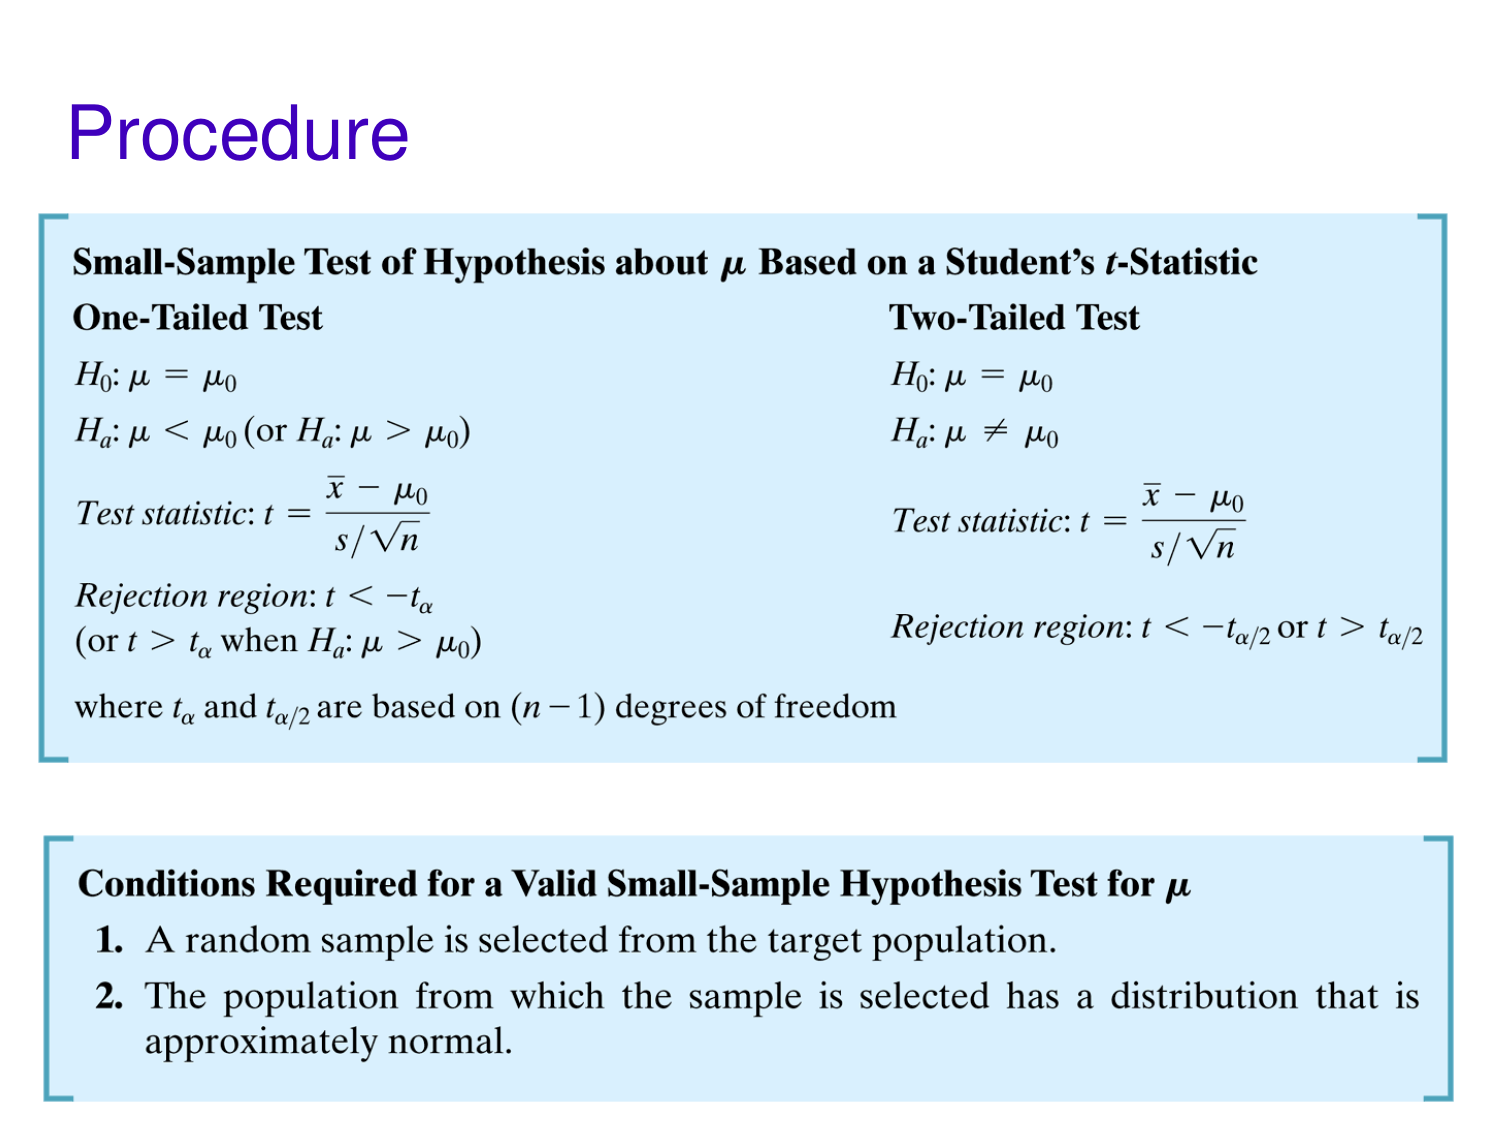
\includegraphics[width=0.78\textwidth]{assets/ch8-t-toets-procedure.png}
  \caption{Stappenplan voor de t-toets (kleine steekproef).}
\end{figure}

\begin{conceptbox}{Waarom $t$ en niet $z$ bij kleine steekproeven?}
Bij kleine $n$ is $s$ geen betrouwbare schatting van $\sigma$. De $t$-verdeling heeft bredere staarten dan de normaalverdeling, wat de extra onzekerheid compenseert. Naarmate $n$ toeneemt, nadert de $t$-verdeling de standaard normaalverdeling.
\end{conceptbox}


\begin{voorbeeld}[Voorbeeld: t-toets voor motoremissie]
Test of een nieuwe motor aan de norm $\mu < 20$ ppm voldoet. Steekproef $n=10$: $\bar{x}=17{,}1$, $s=4{,}7$.

$H_0: \mu = 20$, $H_a: \mu < 20$, $\alpha = 0{,}01$ $\Rightarrow$ $t_{0.01, 9} = -2{,}821$.
$$t = \frac{17{,}1 - 20}{4{,}7/\sqrt{10}} = \frac{-2{,}9}{1{,}486} = -1{,}95$$
$-1{,}95 > -2{,}821$ $\Rightarrow$ verwerp $H_0$ \textbf{niet}. Onvoldoende bewijs dat de motor voldoet.
\end{voorbeeld}

\begin{pyblock}
import numpy as np
from scipy import stats as sts

# Methode 1: als je de ruwe data hebt
data = [15.2, 19.8, 17.0, 18.3, 14.9, 16.1, 20.2, 18.0, 15.8, 17.1]
t_stat, p_two = sts.ttest_1samp(data, popmean=20)
p_eenzijdig = p_two / 2            # linkszijdig als t < 0

# Methode 2: als je enkel xbar, s, n hebt
xbar, mu0, s, n = 17.1, 20, 4.7, 10
t = (xbar - mu0) / (s / np.sqrt(n))
p_links = sts.t.cdf(t, df=n-1)    # P(T < t) -- linkszijdig

# Kritieke waarde:
t_krit = sts.t.ppf(0.01, df=n-1)  # -2.821 voor alpha=0.01 linkszijdig
print(f"t = {t:.3f}, t_krit = {t_krit:.3f}")
\end{pyblock}
\subsection{Toets voor een populatiefractie (grote steekproef)}

Gebruik als $np_0 \geq 15$ en $nq_0 \geq 15$.

\frm{Toetsingsgrootheid $z$ voor $p$}{z = \frac{\hat{p} - p_0}{\sqrt{p_0\,q_0 / n}}}{%
  $\hat{p}$ = steekproeffractie, $p_0$ = getoetste waarde onder $H_0$, $q_0 = 1 - p_0$. Let op: $\sigma_{\hat{p}}$ gebruikt $p_0$ (niet $\hat{p}$), omdat we rekenen onder de aanname dat $H_0$ waar is.}

\begin{figure}[h!]
  \centering
  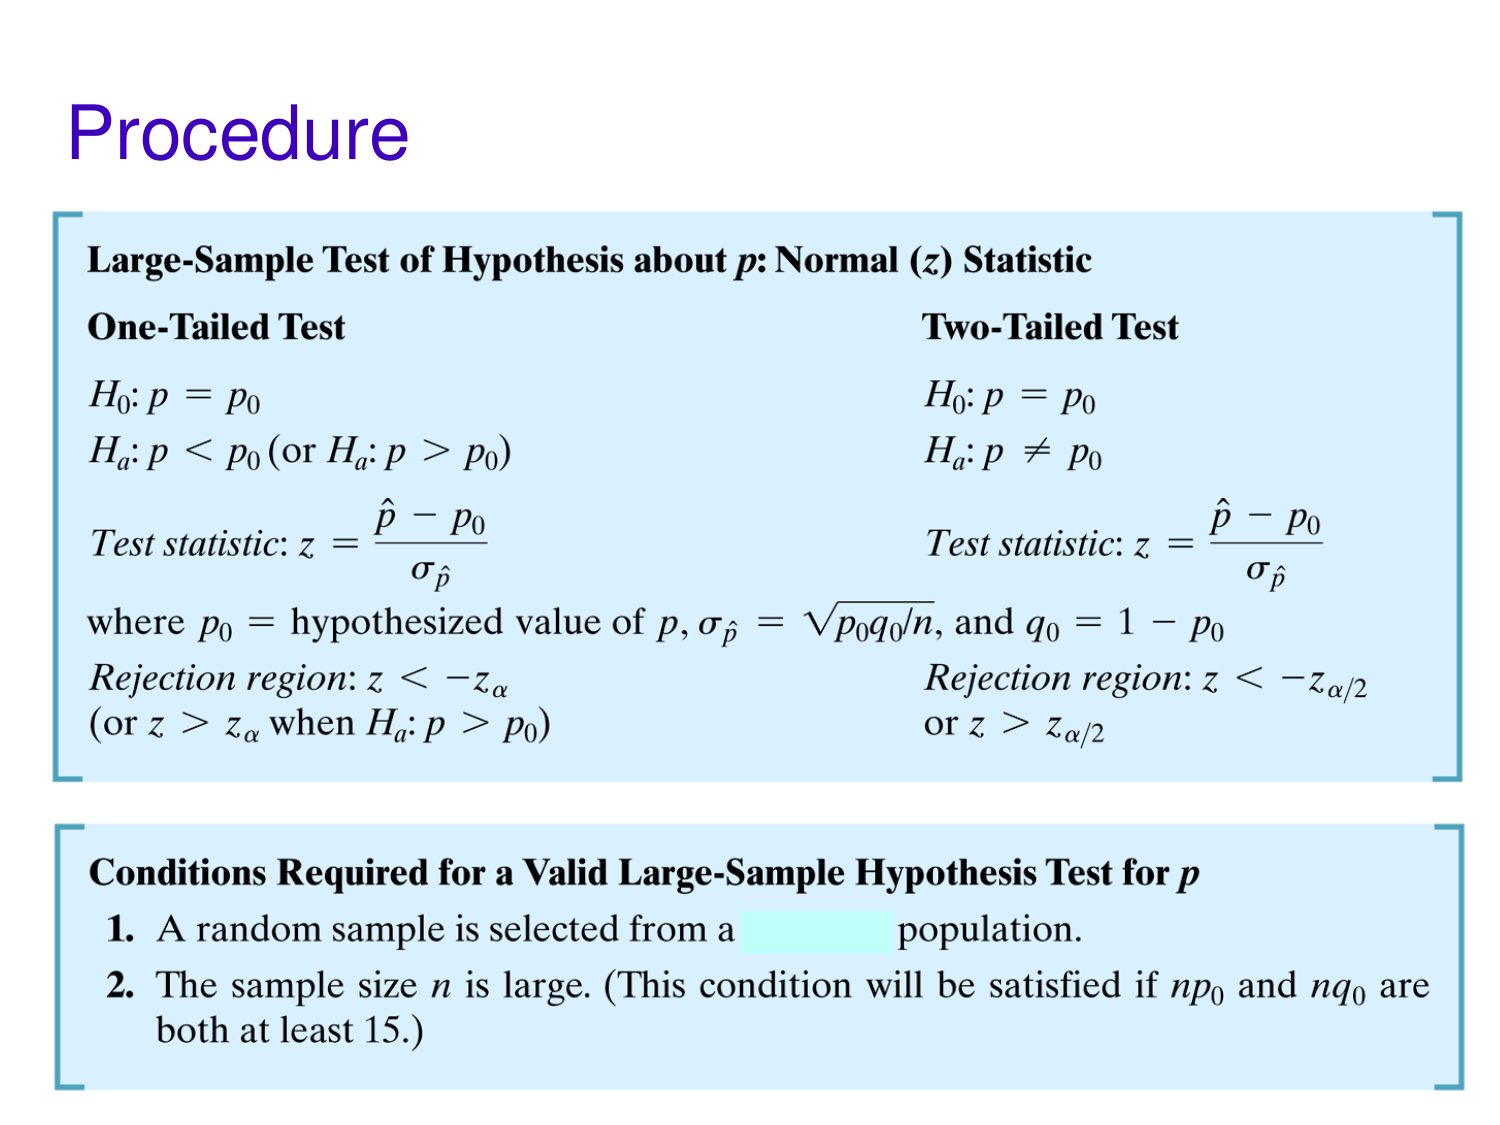
\includegraphics[width=0.78\textwidth]{assets/ch8-proportie-toets-procedure.png}
  \caption{Stappenplan voor de toets over een populatiefractie.}
\end{figure}


\begin{voorbeeld}[Voorbeeld: defecte batterijen (proportietoets)]
Vraag: is de fractie defecte batterijen $< 0{,}05$? Steekproef: $n=300$, $x=9$ defecten ($\hat{p}=0{,}03$).

$H_0: p=0{,}05$, $H_a: p<0{,}05$, $\alpha=0{,}01$. Verificatie: $np_0 = 15 \geq 15$
$$z = \frac{0{,}03 - 0{,}05}{\sqrt{0{,}05 \cdot 0{,}95/300}} = \frac{-0{,}02}{0{,}01258} = -1{,}59$$
$z=-1{,}59 > z_{0.01}=-2{,}33$ $\Rightarrow$ verwerp $H_0$ niet. Onvoldoende bewijs.
\end{voorbeeld}

\begin{pyblock}
import numpy as np
from scipy import stats as sts

phat, p0, n = 0.03, 0.05, 300
z = (phat - p0) / np.sqrt(p0*(1-p0)/n)
print(f"z = {z:.3f}")

p_links = sts.norm.cdf(z)         # linkszijdig (H_a: p < p0)
p_rechts = sts.norm.sf(z)         # rechtszijdig (H_a: p > p0)
p_twee = 2 * sts.norm.cdf(-abs(z))  # tweezijdig

# Kritieke waarde alpha=0.01 linkszijdig: -2.326
z_krit = sts.norm.ppf(0.01)
\end{pyblock}
\subsection{Fout van de tweede soort en onderscheidingsvermogen}

\begin{theorieblok}{$\beta$ berekenen en het onderscheidingsvermogen}
Het \textbf{onderscheidingsvermogen} (\emph{power}) van een toets $= 1 - \beta$ is de kans om $H_0$ correct te verwerpen als $H_a$ waar is.

\medskip
\textbf{Hoe $\beta$ berekenen (grote steekproef, eenzijdige toets):}
\begin{enumerate}
  \item Bepaal de grens van het acceptatiegebied: $\bar{x}_0 = \mu_0 + z_\alpha \cdot \sigma/\sqrt{n}$.
  \item Bereken de $z$-waarde van $\bar{x}_0$ onder de alternatieve verdeling ($\mu = \mu_a$): $z = (\bar{x}_0 - \mu_a)/(\sigma/\sqrt{n})$.
  \item $\beta = P(\bar{x} < \bar{x}_0 \mid \mu = \mu_a) = \Phi(z)$.
\end{enumerate}
Als $\mu_a$ verder van $\mu_0$ ligt, daalt $\beta$ (en stijgt de power).
\end{theorieblok}

\begin{figure}[h!]
  \centering
  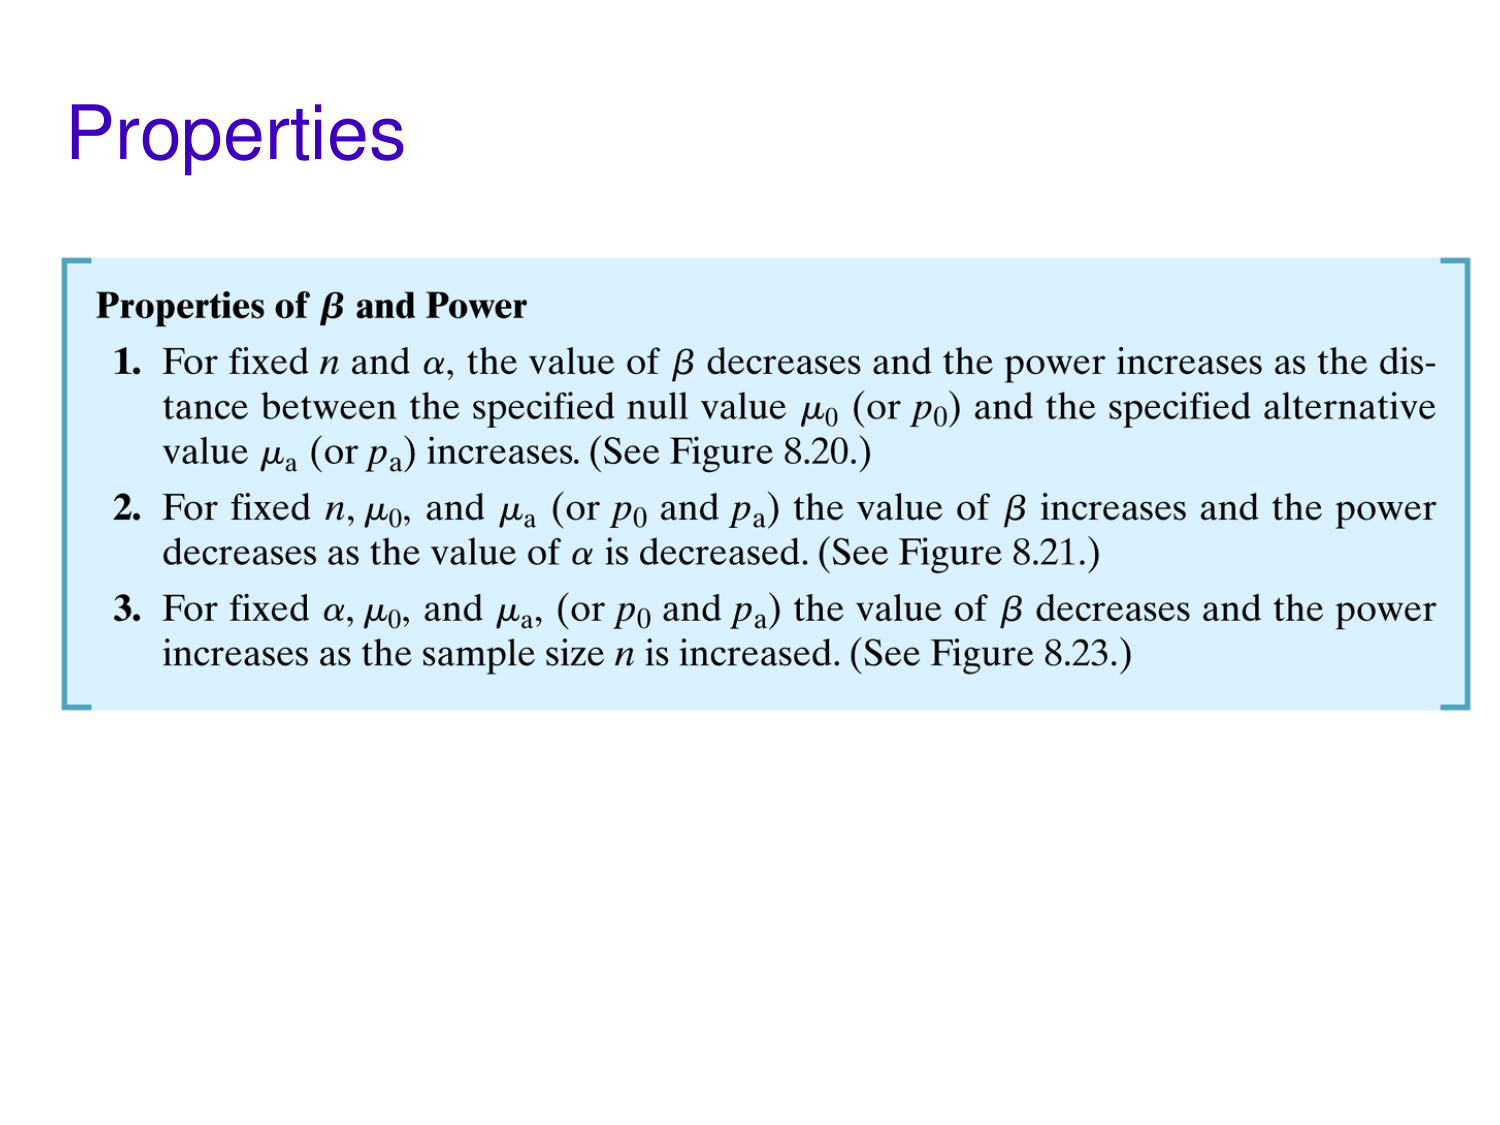
\includegraphics[width=0.72\textwidth]{assets/ch8-eigenschappen-alpha-beta.png}
  \caption{Relatie tussen $\alpha$, $\beta$ en $n$: verlagen van $\alpha$ verhoogt $\beta$; grotere $n$ verlaagt beiden.}
\end{figure}

% =============================================================================
\section{Ch.\ 9 -- Gevolgtrekkingen op basis van twee steekproeven}
% =============================================================================

\begin{conceptbox}{Wanneer gebruik je twee steekproeven?}
Als je twee groepen wil \textbf{vergelijken} -- bijv.\ twee diëten, twee productiemethoden, twee machines -- stel je een parameter voor het \emph{verschil} centraal: $\mu_1 - \mu_2$ of $p_1 - p_2$. Het type methode hangt af van of de steekproeven \emph{onafhankelijk} of \emph{gepaard} zijn.
\end{conceptbox}

\subsection{Vergelijking van twee gemiddelden: onafhankelijke steekproeven}

\subsubsection{Grote steekproeven ($n_1 \geq 30$ en $n_2 \geq 30$)}

\begin{figure}[h!]
  \centering
  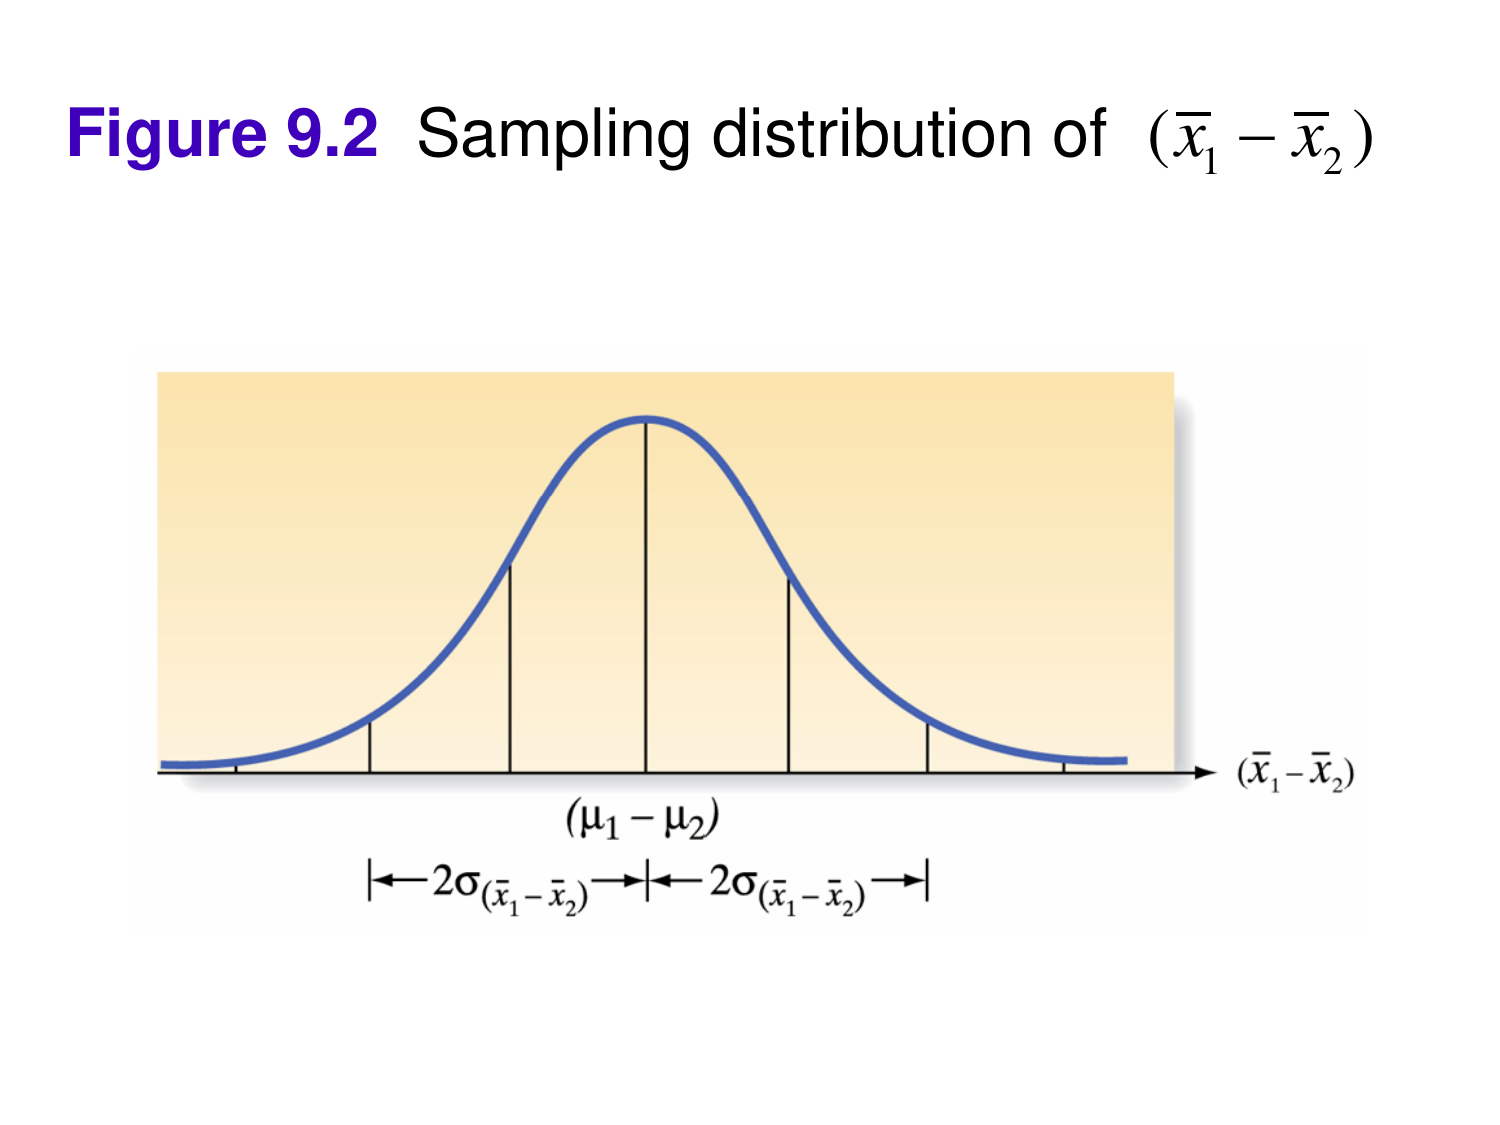
\includegraphics[width=0.75\textwidth]{assets/ch9-steekproeverdeling-verschil.png}
  \caption{Steekproeverdeling van $\bar{x}_1 - \bar{x}_2$ (uit de slides).}
\end{figure}

\frm{Betrouwbaarheidsinterval voor $\mu_1 - \mu_2$ (groot $n$)}{(\bar{x}_1 - \bar{x}_2) \pm z_{\alpha/2}\sqrt{\frac{\sigma_1^2}{n_1} + \frac{\sigma_2^2}{n_2}}}{%
  Gebruik $s_1$ en $s_2$ als schatters voor $\sigma_1$ en $\sigma_2$ als de varianties onbekend zijn. Als nul buiten het interval valt, verschilt $\mu_1$ significant van $\mu_2$.}

\frm{Toetsingsgrootheid $z$ voor $\mu_1 - \mu_2$ (groot $n$)}{z = \frac{(\bar{x}_1 - \bar{x}_2) - D_0}{\sqrt{\dfrac{s_1^2}{n_1} + \dfrac{s_2^2}{n_2}}}}{%
  $D_0$ = getoetste waarde van het verschil onder $H_0$ (meestal 0). Verwerp $H_0: \mu_1 - \mu_2 = D_0$ als $|z| > z_{\alpha/2}$ (tweezijdig).}

\begin{figure}[h!]
  \centering
  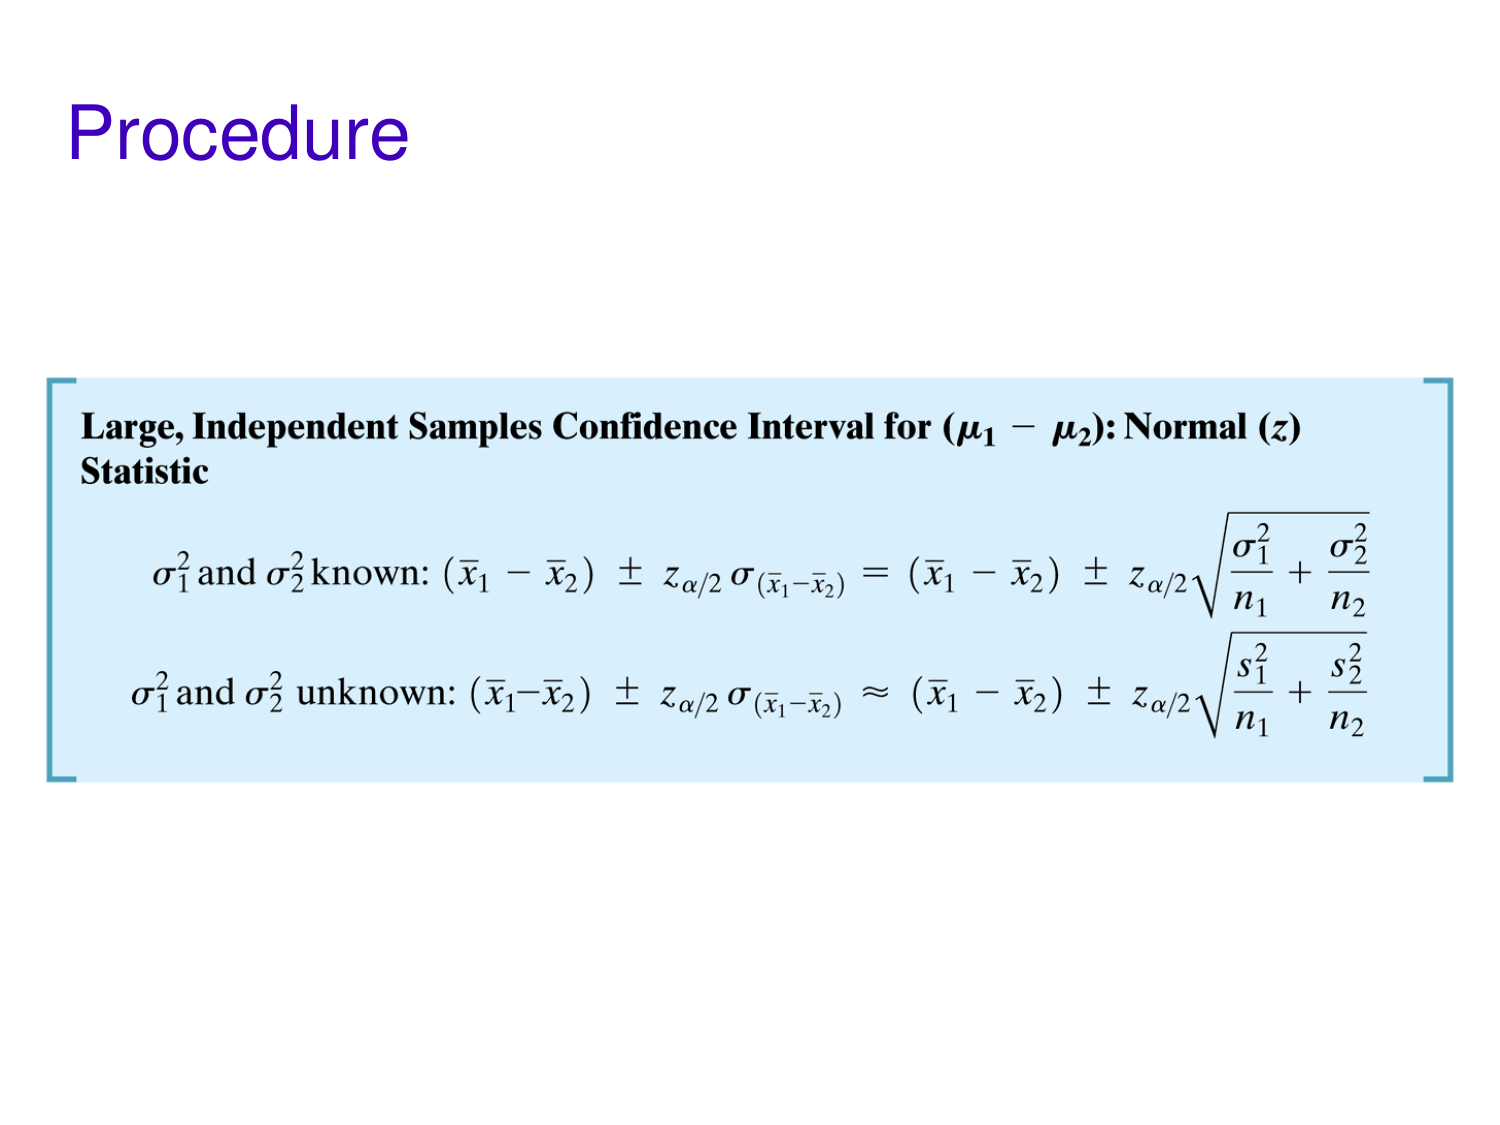
\includegraphics[width=0.78\textwidth]{assets/ch9-CI-grote-steekproef.png}
  \caption{Procedure voor het CI en de toets bij grote onafhankelijke steekproeven.}
\end{figure}


\begin{voorbeeld}[Voorbeeld: gewichtsverlies twee diëten]
Dieet 1: $n_1=42$, $\bar{x}_1=9{,}31$, $s_1=4{,}67$. Dieet 2: $n_2=42$, $\bar{x}_2=7{,}40$, $s_2=4{,}04$.

$H_0: \mu_1-\mu_2=0$, $H_a: \mu_1-\mu_2\neq 0$, $\alpha=0{,}05$.
$$z = \frac{9{,}31 - 7{,}40}{\sqrt{4{,}67^2/42 + 4{,}04^2/42}} = \frac{1{,}91}{0{,}618} = 3{,}09$$
$p = 2(1-\Phi(3{,}09)) = 0{,}002 < 0{,}05$ $\Rightarrow$ verwerp $H_0$. Diëten verschillen significant.
\end{voorbeeld}

\begin{pyblock}
import numpy as np
from scipy import stats as sts

# Als je enkel xbar, s, n hebt:
x1bar, s1, n1 = 9.31, 4.67, 42
x2bar, s2, n2 = 7.40, 4.04, 42
z = (x1bar - x2bar) / np.sqrt(s1**2/n1 + s2**2/n2)
p = 2 * sts.norm.sf(abs(z))
print(f"z = {z:.3f}, p = {p:.4f}")

# Als je ruwe data hebt (kleine n):
# Gelijke varianties (pooled):
t, p = sts.ttest_ind(data1, data2, equal_var=True)
# Ongelijke varianties (Welch - veiliger):
t, p = sts.ttest_ind(data1, data2, equal_var=False)

# CI voor mu1 - mu2:
diff = x1bar - x2bar
marge = sts.norm.ppf(0.975) * np.sqrt(s1**2/n1 + s2**2/n2)
print(f"95% CI: ({diff-marge:.2f}, {diff+marge:.2f})")
\end{pyblock}
\subsubsection{Kleine steekproeven ($n_1 < 30$ of $n_2 < 30$)}

Aannames: beide populaties normaal verdeeld, gelijke (maar onbekende) varianties, steekproeven onafhankelijk.



\frm{Gepoolde variantie $s_p^2$}{s_p^2 = \frac{(n_1-1)s_1^2 + (n_2-1)s_2^2}{n_1 + n_2 - 2}}{%
  Gewogen gemiddelde van de twee steekproefvarianties. Vrijheidsgraden $= n_1 + n_2 - 2$.}

\frm{T-toets voor $\mu_1 - \mu_2$ (klein $n$, gelijke varianties)}{t = \frac{(\bar{x}_1 - \bar{x}_2) - D_0}{s_p\sqrt{\dfrac{1}{n_1} + \dfrac{1}{n_2}}}}{%
  $t$-verdeling met $\nu = n_1 + n_2 - 2$ vrijheidsgraden. BI: $(\bar{x}_1 - \bar{x}_2) \pm t_{\alpha/2}\,s_p\sqrt{1/n_1 + 1/n_2}$.}

\begin{figure}[h!]
  \centering
  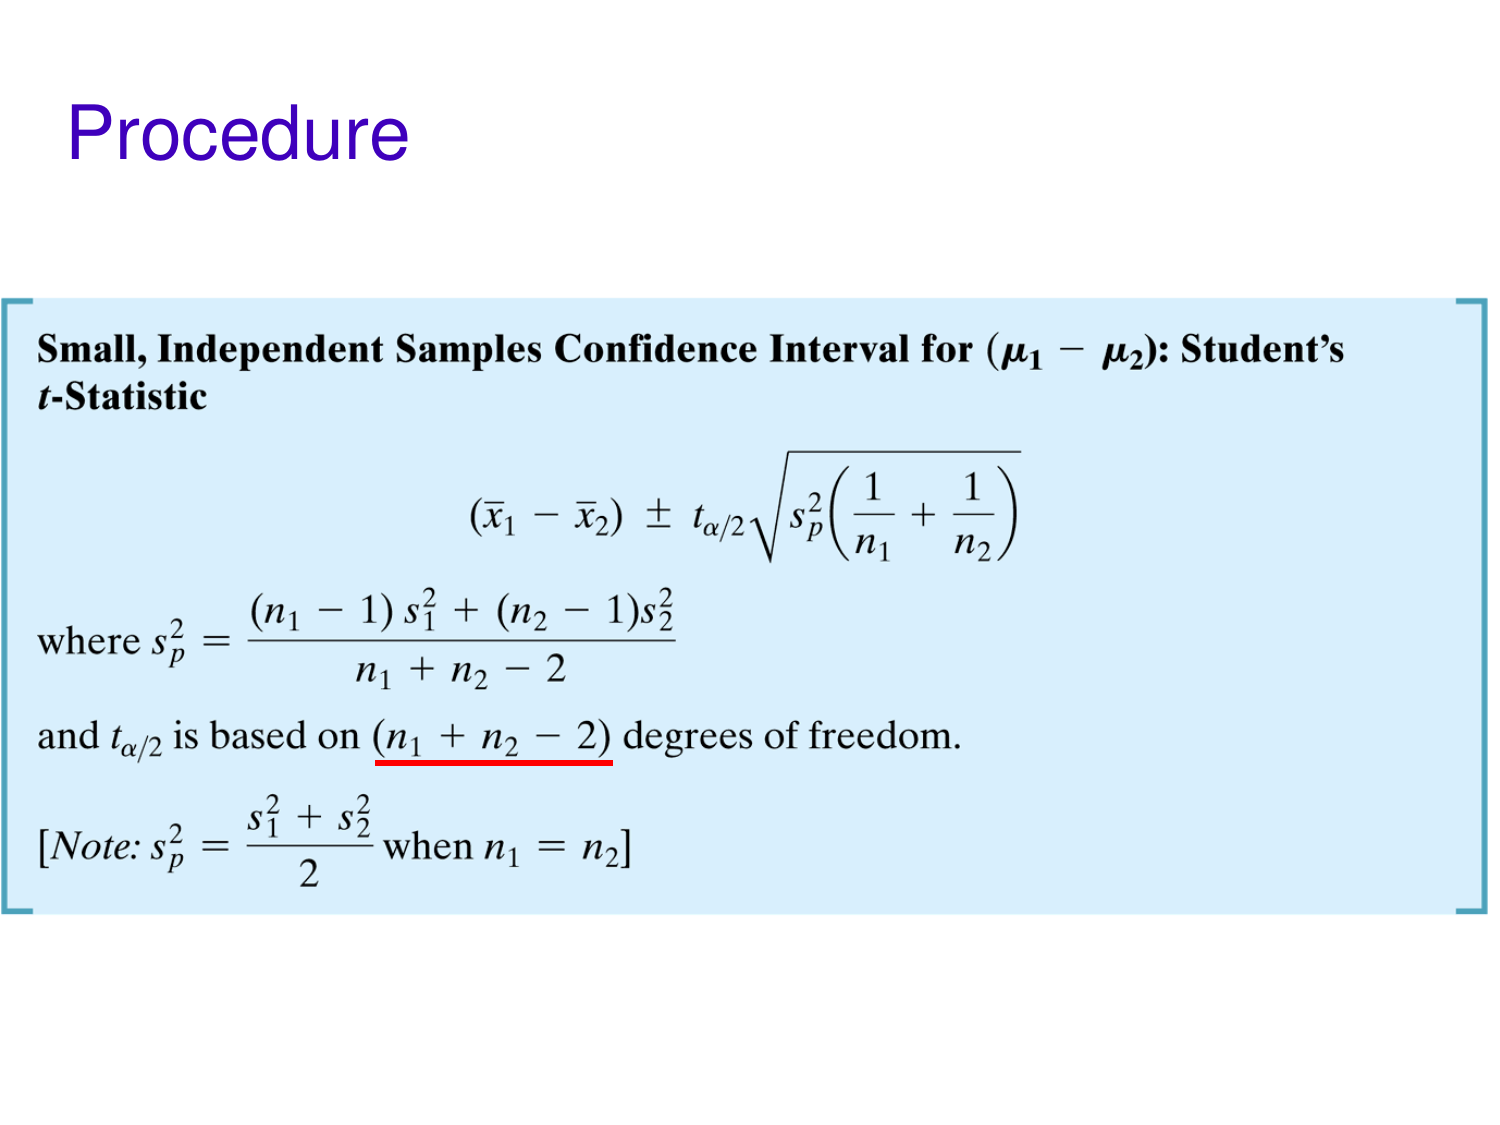
\includegraphics[width=0.78\textwidth]{assets/ch9-t-toets-twee-steekproeven.png}
  \caption{Stappenplan voor de twee-steekproef $t$-toets (kleine steekproeven).}
\end{figure}

\begin{examenbox}
Als nul \emph{binnen} het BI valt $\Rightarrow$ onvoldoende bewijs dat $\mu_1 \neq \mu_2$. Het BI geeft meer informatie dan de hypothesetoets alleen (het toont ook de \emph{grootte} van het verschil).
\end{examenbox}

\subsection{Gepaarde waarnemingen}

\begin{conceptbox}{Wanneer gebruik je gepaarde waarnemingen?}
Als de twee metingen \textbf{niet onafhankelijk} zijn -- bijv.\ dezelfde persoon vóór en na een behandeling, of twee methoden getest op hetzelfde object -- dan zijn de steekproeven \emph{gepaard}. Je analyseert de \textbf{verschillen} $d_i = x_{1i} - x_{2i}$ als een enkele steekproef.

\medskip
\textbf{Voordeel:} Door het koppelen elimineer je storende variabiliteit (bijv.\ verschillen tussen personen), waardoor de toets gevoeliger wordt.
\end{conceptbox}

\begin{figure}[h!]
  \centering
  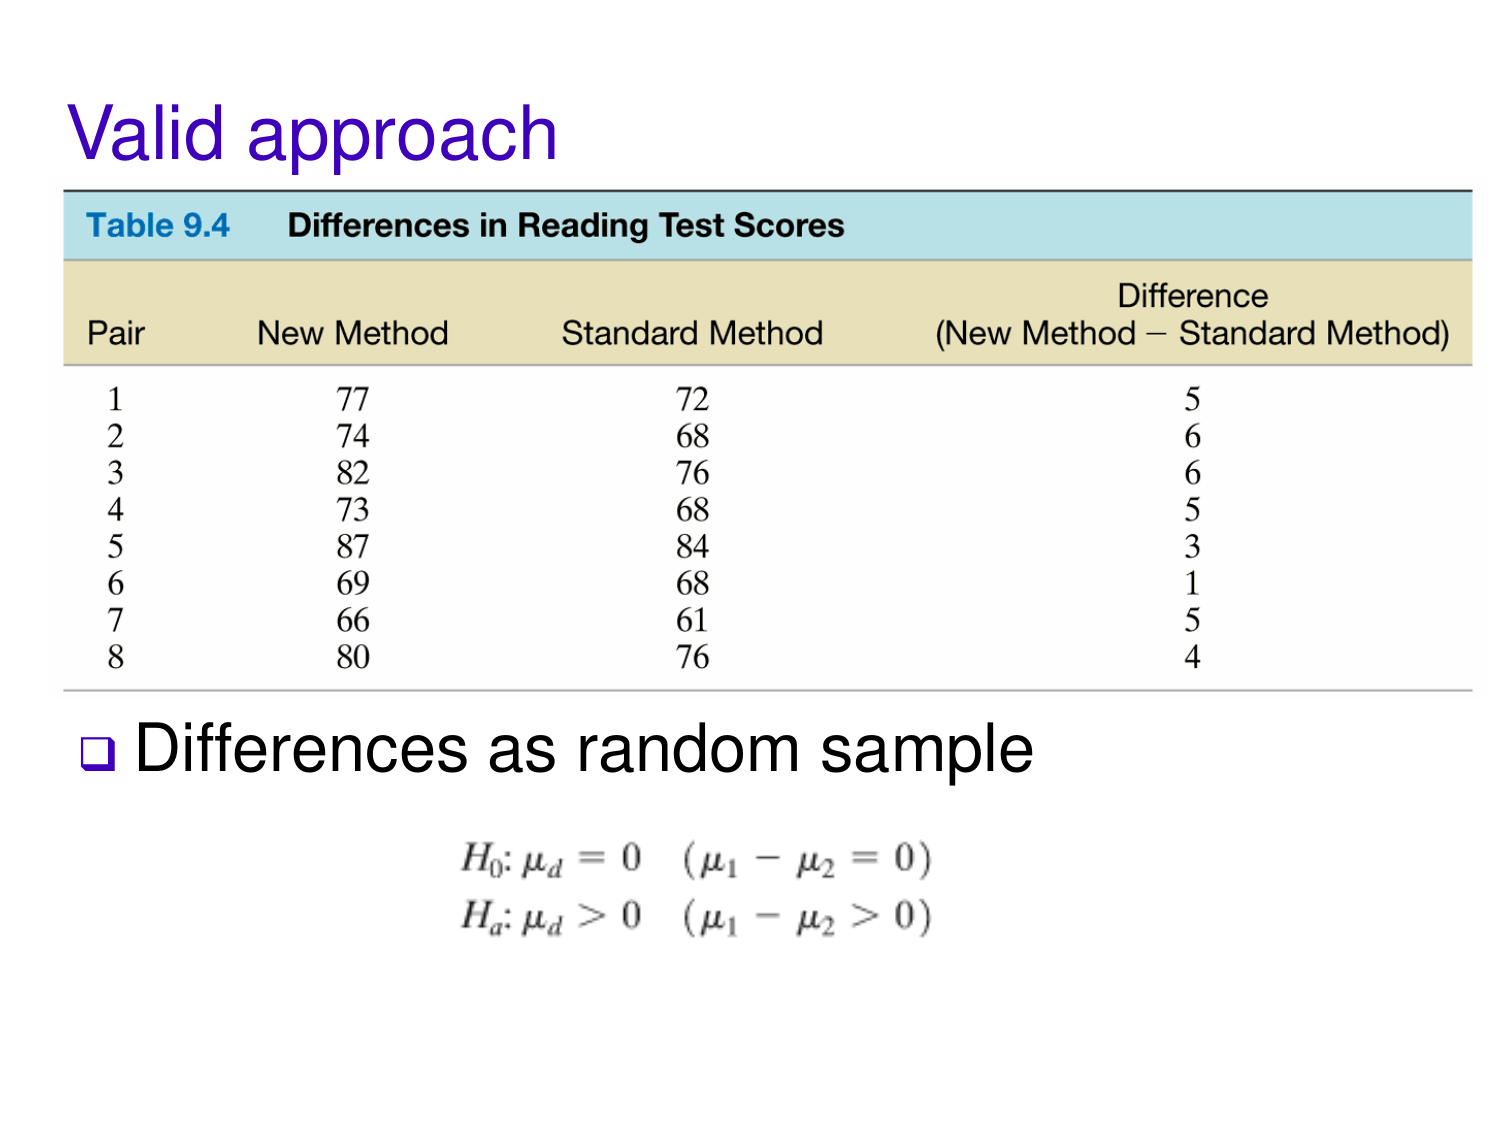
\includegraphics[width=0.75\textwidth]{assets/ch9-gepaarde-waarnemingen.png}
  \caption{Bij gepaarde waarnemingen analyseer je de individuele verschillen $d_i$.}
\end{figure}

\frm{Gemiddeld verschil en standaardafwijking}{%
  \bar{d} = \frac{\displaystyle\sum_{i=1}^{n} d_i}{n}, \quad
  s_d = \sqrt{\frac{\displaystyle\sum (d_i - \bar{d})^2}{n-1}}}{%
  $n$ = aantal paren. Aanname: de verschillen $d_i$ zijn normaal verdeeld (geen aanname van gelijke varianties nodig).}

\frm{T-toets voor gepaarde waarnemingen}{t = \frac{\bar{d} - D_0}{s_d / \sqrt{n}}}{%
  $t$-verdeling met $\nu = n - 1$ vrijheidsgraden. BI: $\bar{d} \pm t_{\alpha/2}\,s_d/\sqrt{n}$.}

\begin{figure}[h!]
  \centering
  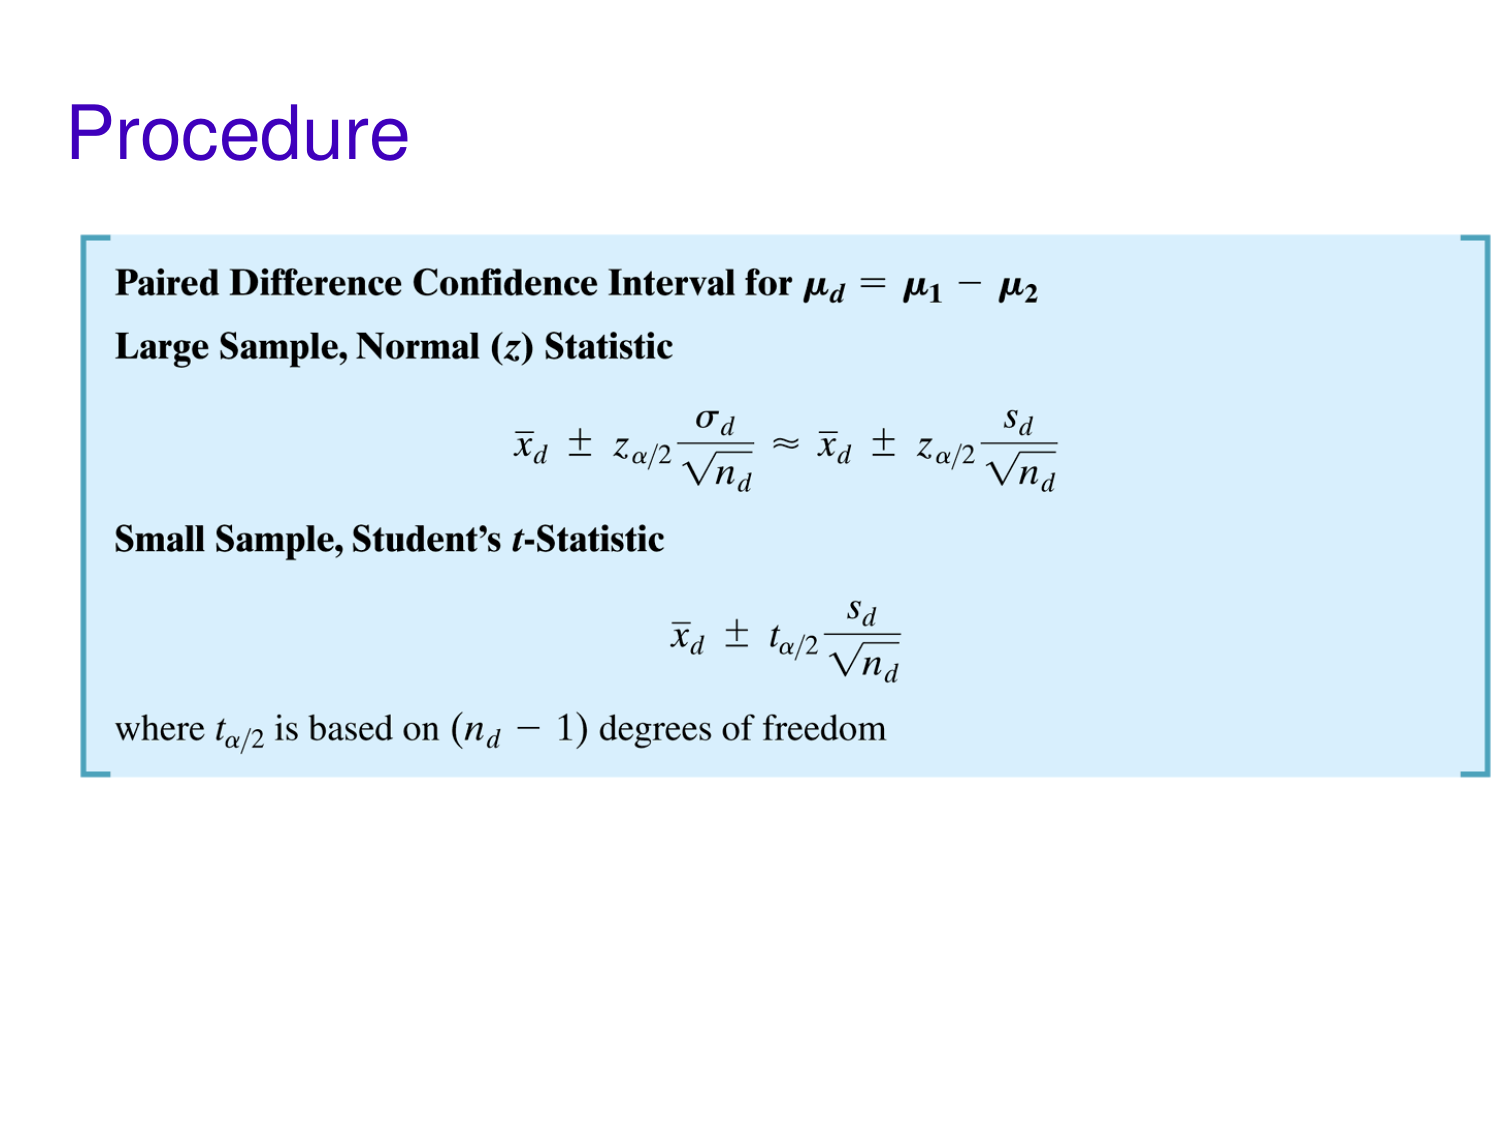
\includegraphics[width=0.78\textwidth]{assets/ch9-procedure-gepaard.png}
  \caption{Stappenplan voor de gepaarde $t$-toets.}
\end{figure}


\begin{voorbeeld}[Voorbeeld: leesmethoden vergeleken (gepaard)]
8 koppels van gelijkwaardige leerlingen ($n=8$). Nieuwe methode vs.\ standaard. Verschillen $d_i$: $5, 6, 6, 5, 3, 1, 5, 4$.
$\bar{d}=4{,}375$, $s_d=1{,}685$.

$H_0: \mu_d=0$, $H_a: \mu_d>0$, $\alpha=0{,}05$. $t_{0.05,7}=1{,}895$.
$$t = \frac{4{,}375}{1{,}685/\sqrt{8}} = \frac{4{,}375}{0{,}596} = 7{,}34$$
$7{,}34 > 1{,}895$ $\Rightarrow$ verwerp $H_0$. Nieuwe methode is significant beter.
\end{voorbeeld}

\begin{pyblock}
import numpy as np
from scipy import stats as sts

nieuw    = [77, 74, 82, 73, 87, 69, 66, 80]
standaard = [72, 68, 76, 68, 84, 68, 61, 76]

# Methode 1: scipy direct
t, p = sts.ttest_rel(nieuw, standaard)
p_eenzijdig = p / 2               # als t > 0 en H_a: mu_d > 0

# Methode 2: handmatig via differences
d = np.array(nieuw) - np.array(standaard)
dbar, sd, n = d.mean(), d.std(ddof=1), len(d)
t_hand = (dbar - 0) / (sd / np.sqrt(n))
print(f"t = {t_hand:.3f}")

# CI voor mu_d:
t_krit = sts.t.ppf(0.975, df=n-1)
marge = t_krit * sd / np.sqrt(n)
print(f"95% CI: ({dbar-marge:.3f}, {dbar+marge:.3f})")
\end{pyblock}
\subsection{Vergelijking van twee fracties (grote steekproeven)}

\frm{Betrouwbaarheidsinterval voor $p_1 - p_2$}{(\hat{p}_1 - \hat{p}_2) \pm z_{\alpha/2}\sqrt{\frac{\hat{p}_1\hat{q}_1}{n_1} + \frac{\hat{p}_2\hat{q}_2}{n_2}}}{%
  $\hat{q}_i = 1 - \hat{p}_i$. Geldig als $n_i\hat{p}_i \geq 15$ en $n_i\hat{q}_i \geq 15$.}

\frm{Toetsingsgrootheid $z$ voor $p_1 - p_2$ (bij $H_0: p_1 = p_2$)}{z = \frac{(\hat{p}_1 - \hat{p}_2)}{\sqrt{\hat{p}\,\hat{q}\!\left(\dfrac{1}{n_1} + \dfrac{1}{n_2}\right)}}}{%
  $\hat{p} = \dfrac{x_1 + x_2}{n_1 + n_2}$ = gepoolde schatting van $p$ (beste schatting als $H_0: p_1 = p_2$ geldt). $\hat{q} = 1 - \hat{p}$.}

\begin{figure}[h!]
  \centering
  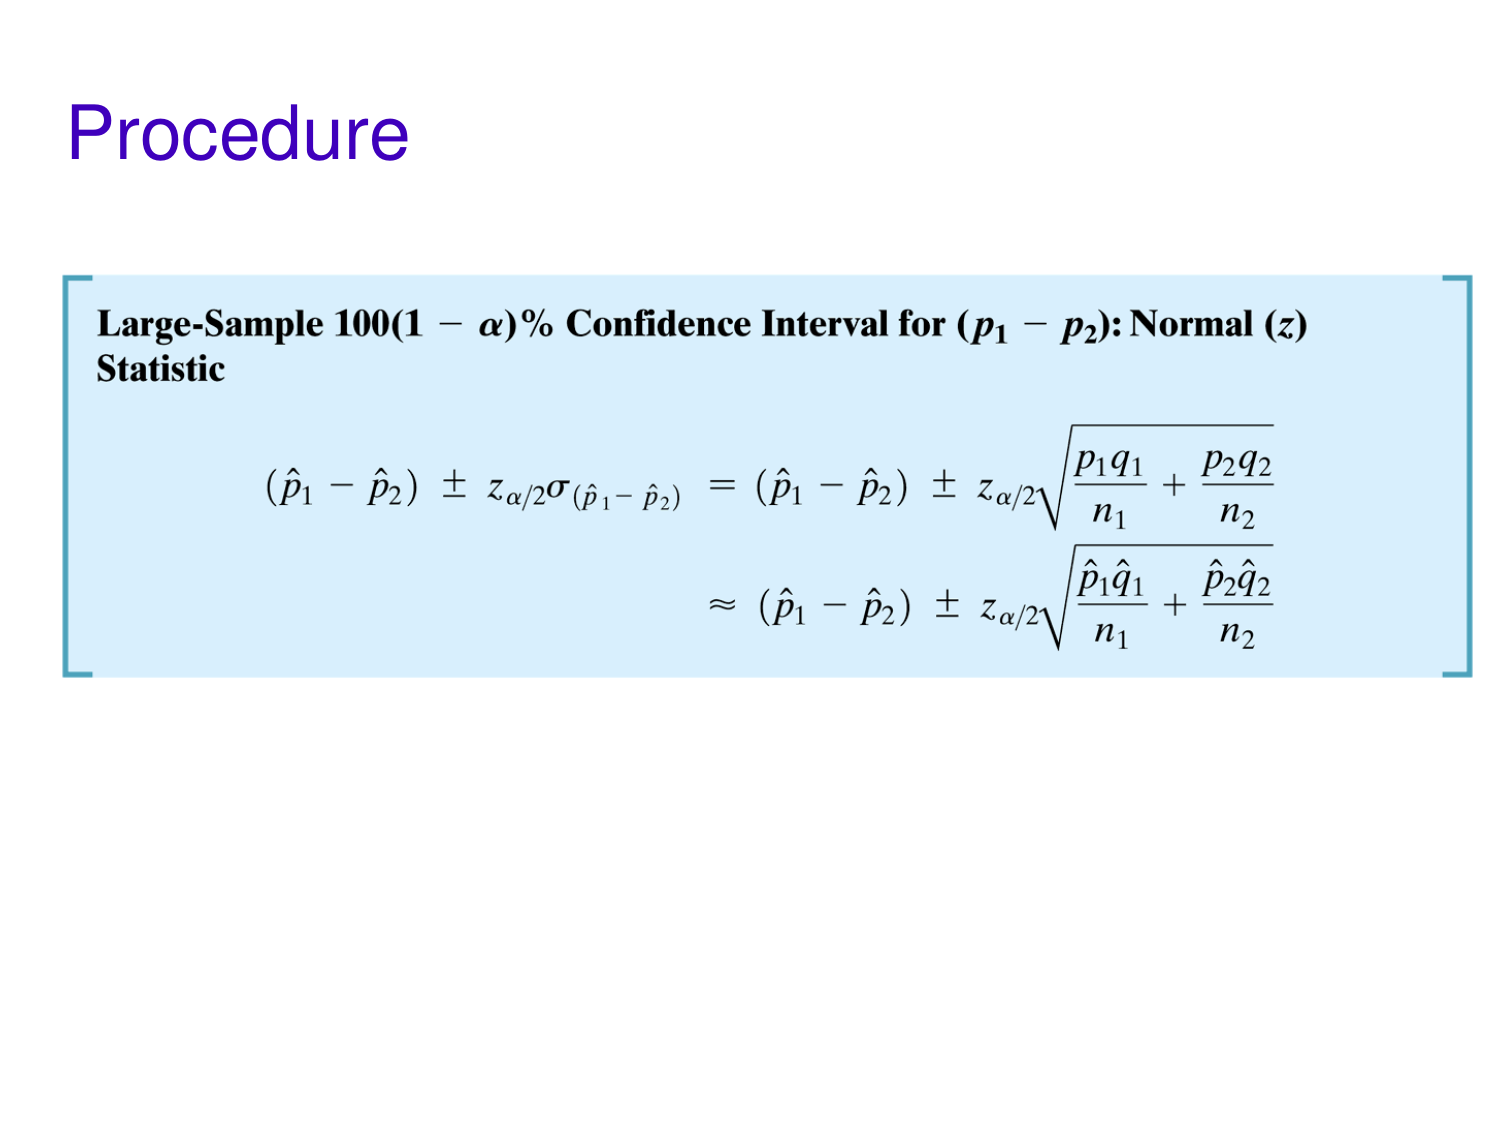
\includegraphics[width=0.78\textwidth]{assets/ch9-CI-twee-fracties.png}
  \caption{Stappenplan voor het CI en de toets voor twee fracties.}
\end{figure}


\begin{pyblock}
import numpy as np
from scipy import stats as sts

# Gegevens
n1, x1 = 1000, 155                 # regio 1
n2, x2 = 1000, 128                 # regio 2
phat1, phat2 = x1/n1, x2/n2

# CI voor p1 - p2:
alpha = 0.05
z = sts.norm.ppf(1 - alpha/2)
marge = z * np.sqrt(phat1*(1-phat1)/n1 + phat2*(1-phat2)/n2)
print(f"95% CI: ({phat1-phat2-marge:.4f}, {phat1-phat2+marge:.4f})")

# Toets H_0: p1 = p2 (pooled schatting van p):
phat_pool = (x1 + x2) / (n1 + n2)
z_toets = (phat1 - phat2) / np.sqrt(phat_pool*(1-phat_pool)*(1/n1 + 1/n2))
p_rechts = sts.norm.sf(z_toets)
print(f"z = {z_toets:.3f}, p = {p_rechts:.4f}")
\end{pyblock}
\subsection{Vergelijking van twee varianties: de F-toets}

\begin{conceptbox}{Wanneer gebruik je de F-toets?}
De $t$-toets voor kleine steekproeven veronderstelt \emph{gelijke varianties}. Je kan dit controleren (of testen) met de \textbf{F-toets}. Ook nuttig om de precisie van twee meetinstrumenten te vergelijken.
\end{conceptbox}

\begin{figure}[h!]
  \centering
  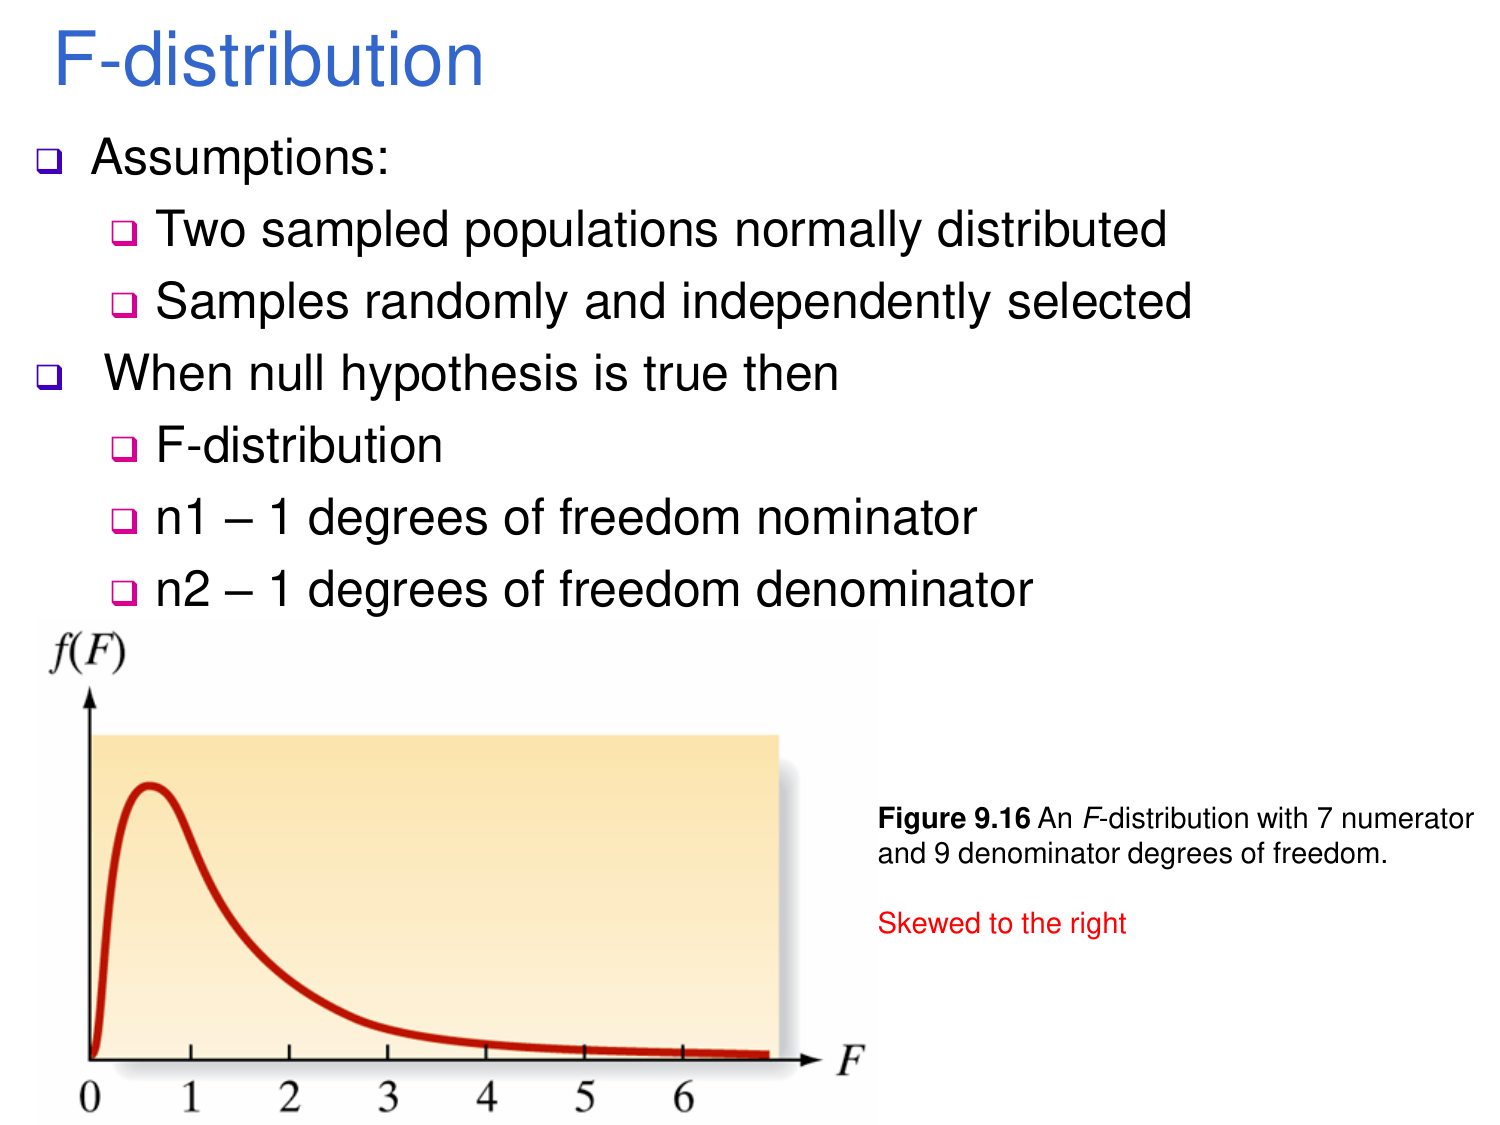
\includegraphics[width=0.75\textwidth]{assets/ch9-F-verdeling.png}
  \caption{De F-verdeling is rechtsscheef. Vrijheidsgraden: teller $n_1-1$, noemer $n_2-1$.}
\end{figure}

\frm{F-toetsingsgrootheid voor $\sigma_1^2 / \sigma_2^2$}{F = \frac{s_1^2}{s_2^2}}{%
  Zet de \emph{grootste} steekproefvariantie in de teller. Verdeling: $F$ met $\nu_1 = n_1 - 1$ en $\nu_2 = n_2 - 1$ vrijheidsgraden. Verwerp $H_0: \sigma_1^2 = \sigma_2^2$ als $F > F_{\alpha/2, \nu_1, \nu_2}$.}

\begin{figure}[h!]
  \centering
  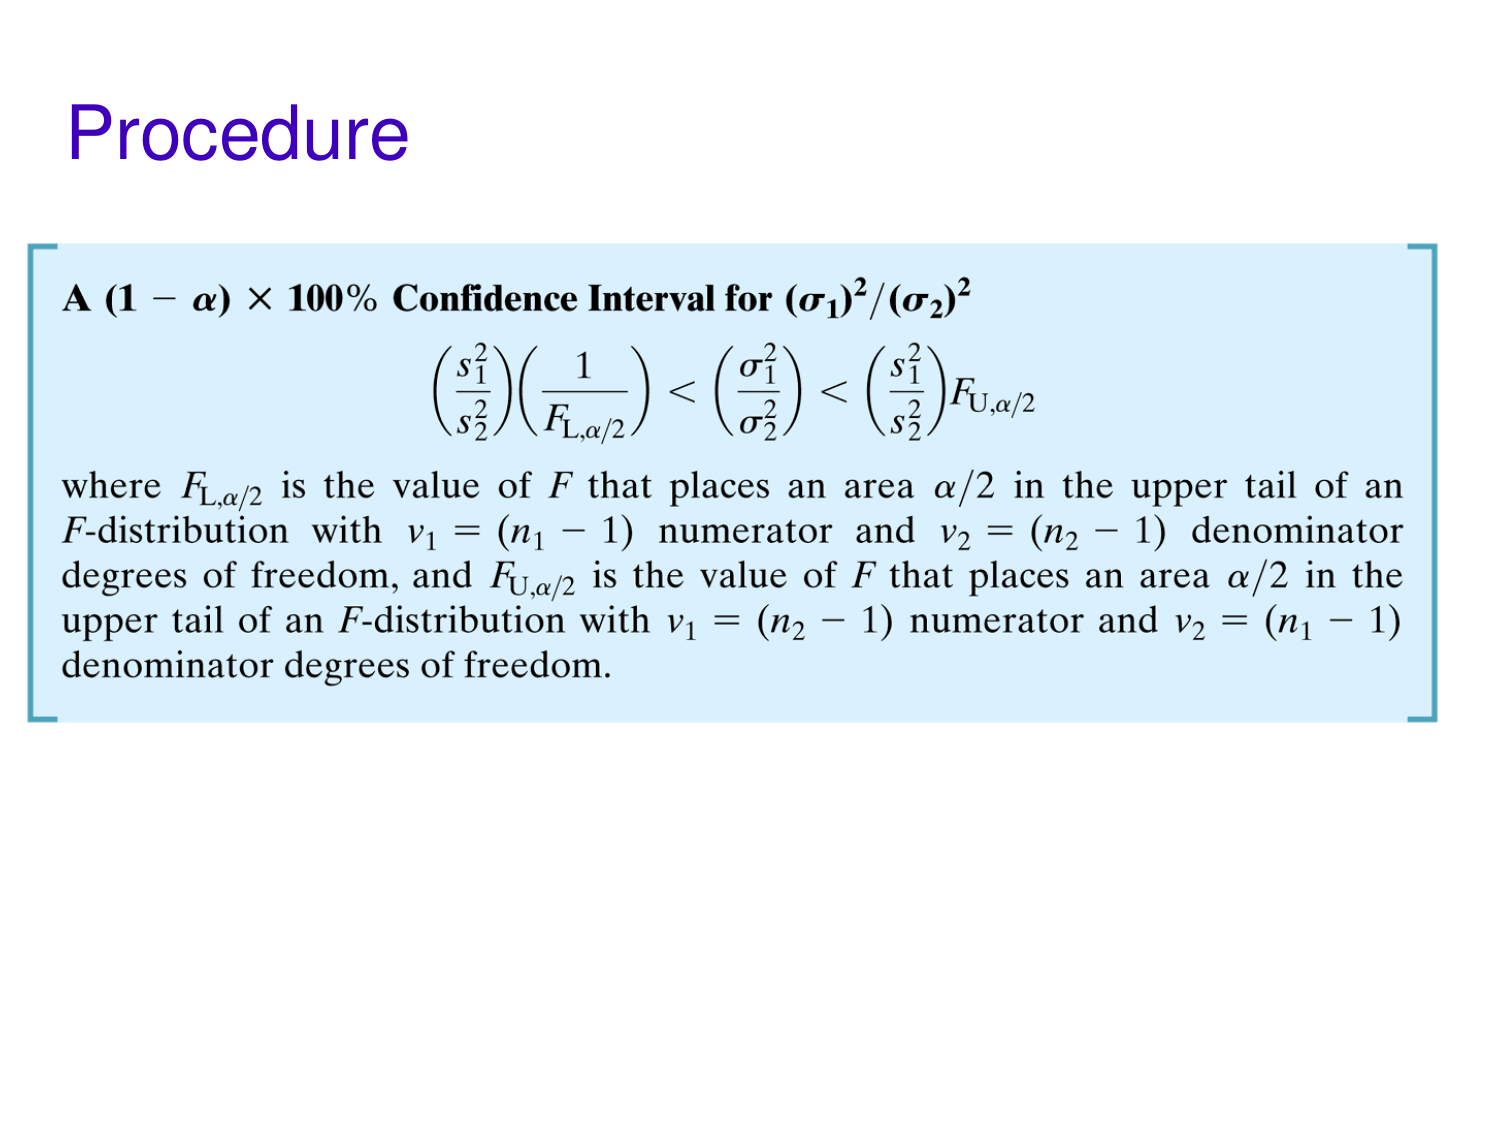
\includegraphics[width=0.78\textwidth]{assets/ch9-F-toets-procedure.png}
  \caption{Stappenplan voor de F-toets (vergelijking van twee varianties).}
\end{figure}

\begin{examenbox}
Bij de tweezijdige F-toets: zet altijd de grootste $s^2$ in de teller, en gebruik dan $\alpha/2$ als drempel (zodat de echte $\alpha$ weer $\alpha$ wordt). In Python: \texttt{sts.f.ppf(0.975, n1-1, n2-1)}.
\end{examenbox}

% =============================================================================

\begin{voorbeeld}[Voorbeeld: variantietoets voor muizen (F-toets)]
Leverancier 1: $n_1=13$, $s_1^2=0{,}0409$. Leverancier 2: $n_2=18$, $s_2^2=0{,}00964$.
$H_0: \sigma_1^2=\sigma_2^2$, $H_a: \sigma_1^2 \neq \sigma_2^2$, $\alpha=0{,}10$.

Grootste variantie in teller: $F = 0{,}0409/0{,}00964 = 4{,}24$.
Drempel bij $\alpha/2=0{,}05$: $F_{0{,}05; 12; 17}=2{,}38$. Verwerp $H_0$.
\end{voorbeeld}

\begin{pyblock}
import numpy as np
from scipy import stats as sts

# Altijd grootste variantie in teller:
s1sq, n1 = 0.0409, 13
s2sq, n2 = 0.00964, 18

F = s1sq / s2sq                    # s1^2 > s2^2
df1, df2 = n1-1, n2-1
p = 2 * sts.f.sf(F, df1, df2)     # tweezijdig
print(f"F = {F:.3f}, p = {p:.4f}")

# Kritieke waarde (alpha=0.10 tweezijdig => alpha/2=0.05):
F_krit = sts.f.ppf(0.95, df1, df2)
print(f"F_krit = {F_krit:.3f}")

# Met ruwe data:
# stat = np.var(data1,ddof=1)/np.var(data2,ddof=1)
# p = 2*min(sts.f.cdf(stat,df1,df2), sts.f.sf(stat,df1,df2))
\end{pyblock}
\section{Ch.\ 10 -- Variantieanalyse (ANOVA)}
% =============================================================================

\begin{conceptbox}{Wat is ANOVA?}
\textbf{Variantieanalyse} (Analysis of Variance, ANOVA) vergelijkt de gemiddelden van \textbf{meer dan twee groepen} tegelijk. Je toetst of minstens één groepsgemiddelde significant verschilt van de andere.

\medskip
\textbf{Kernidee:} als de variabiliteit \emph{tussen} de groepen groot is in verhouding tot de variabiliteit \emph{binnen} de groepen, dan wijken de gemiddelden waarschijnlijk echt van elkaar af.
\end{conceptbox}

\subsection{Begrippen in experimenteel ontwerp}



\begin{theorieblok}{Terminologie}
\begin{itemize}
  \item \textbf{Responsvariabele} (\emph{response variable}): de afhankelijke variabele die je meet (bijv.\ afstand golfbal).
  \item \textbf{Factor}: een verklarende variabele (bijv.\ merk golfbal). Kan kwalitatief of kwantitatief zijn.
  \item \textbf{Niveaus} (\emph{levels}): de waarden die een factor aanneemt (bijv.\ merk A, B, C, D).
  \item \textbf{Behandeling} (\emph{treatment}): een specifieke combinatie van factorniveaus.
  \item \textbf{Experimentele eenheid}: het object waarop een behandeling wordt toegepast.
  \item \textbf{Volledig gerandomiseerd ontwerp}: experimentele eenheden worden \emph{willekeurig} toebedeeld aan behandelingen.
\end{itemize}
\end{theorieblok}

\subsection{De F-toets in het volledig gerandomiseerde ontwerp}

Gegeven $k$ behandelingen, elk met $n_i$ observaties, en totaal $n = \sum n_i$ observaties.

\begin{figure}[h!]
  \centering
  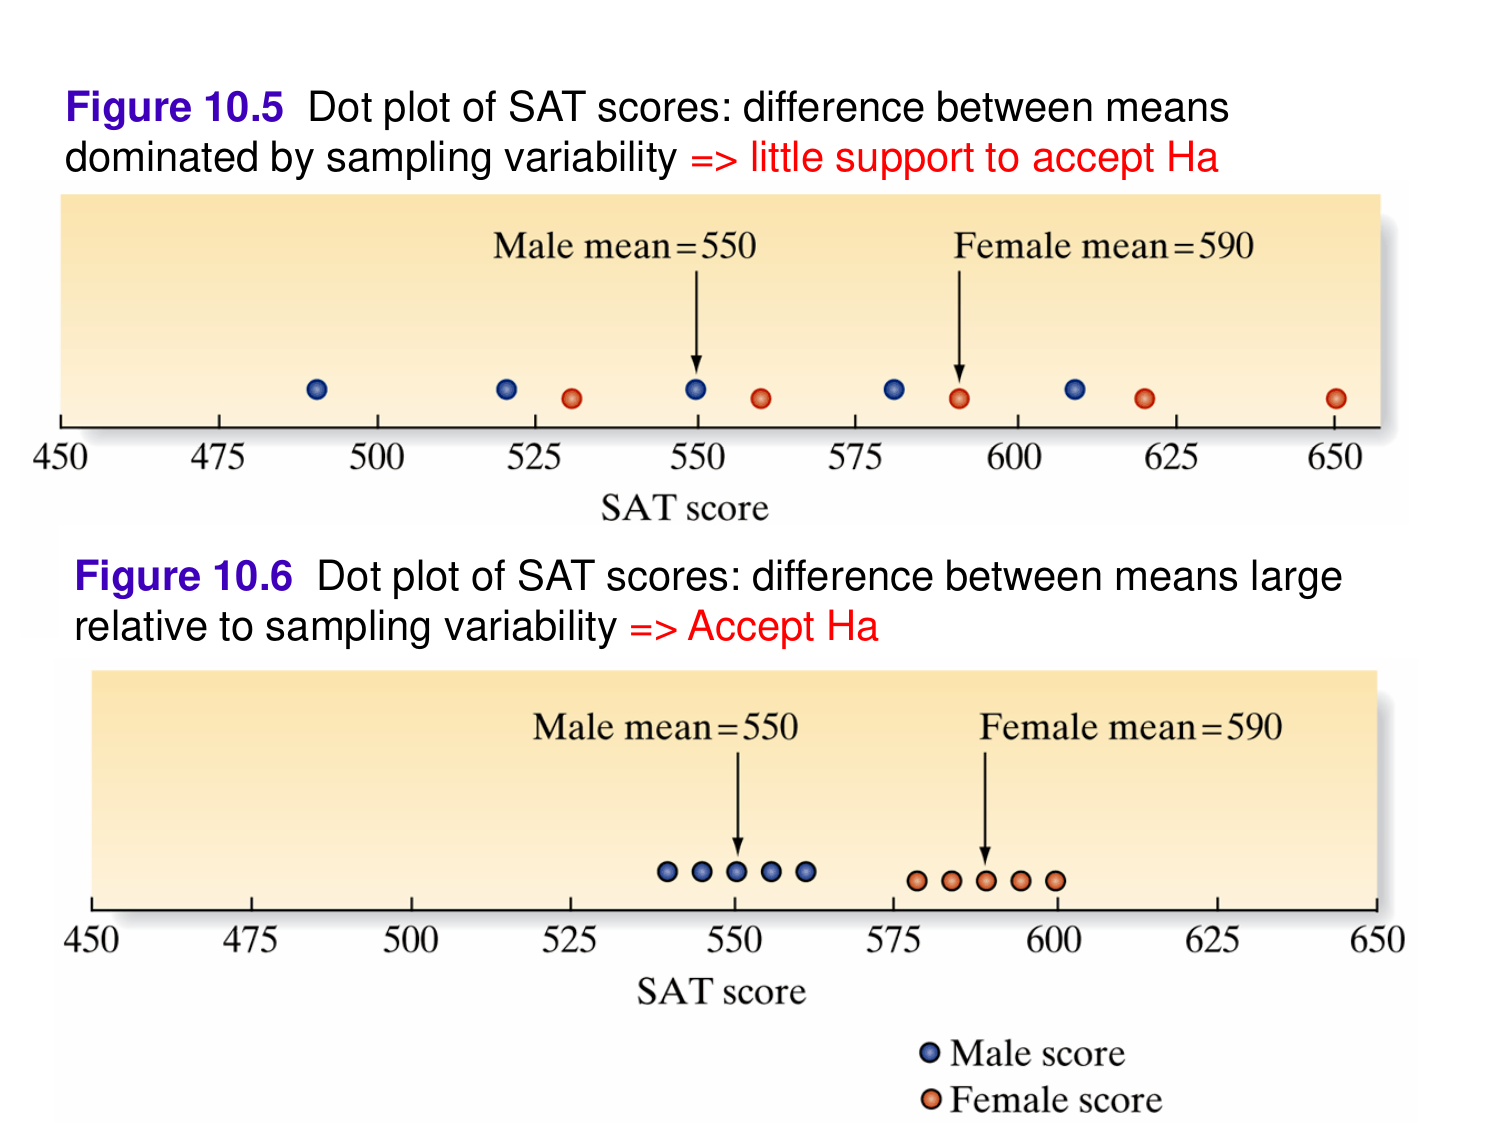
\includegraphics[width=0.72\textwidth]{assets/ch10-variabiliteit-tussen-groepen.png}
  \caption{Vergelijking van situaties: links weinig bewijs voor $H_a$ (grote steekproefvariabiliteit), rechts sterk bewijs (kleine steekproefvariabiliteit).}
\end{figure}

\frm{Kwadratensom behandelingen (SST)}{SST = \sum_{i=1}^{k} n_i (\bar{x}_i - \bar{x})^2}{%
  Maatstaf voor variabiliteit \emph{tussen} de behandelingsgemiddelden. $\bar{x}_i$ = gemiddelde van behandeling $i$, $\bar{x}$ = overall gemiddelde.}

\frm{Kwadratensom fout (SSE)}{SSE = \sum_{i=1}^{k} (n_i - 1) s_i^2}{%
  Maatstaf voor variabiliteit \emph{binnen} de behandelingen (niet verklaard door de factor). $s_i^2$ = steekproefvariantie van behandeling $i$.}

\begin{figure}[h!]
  \centering
  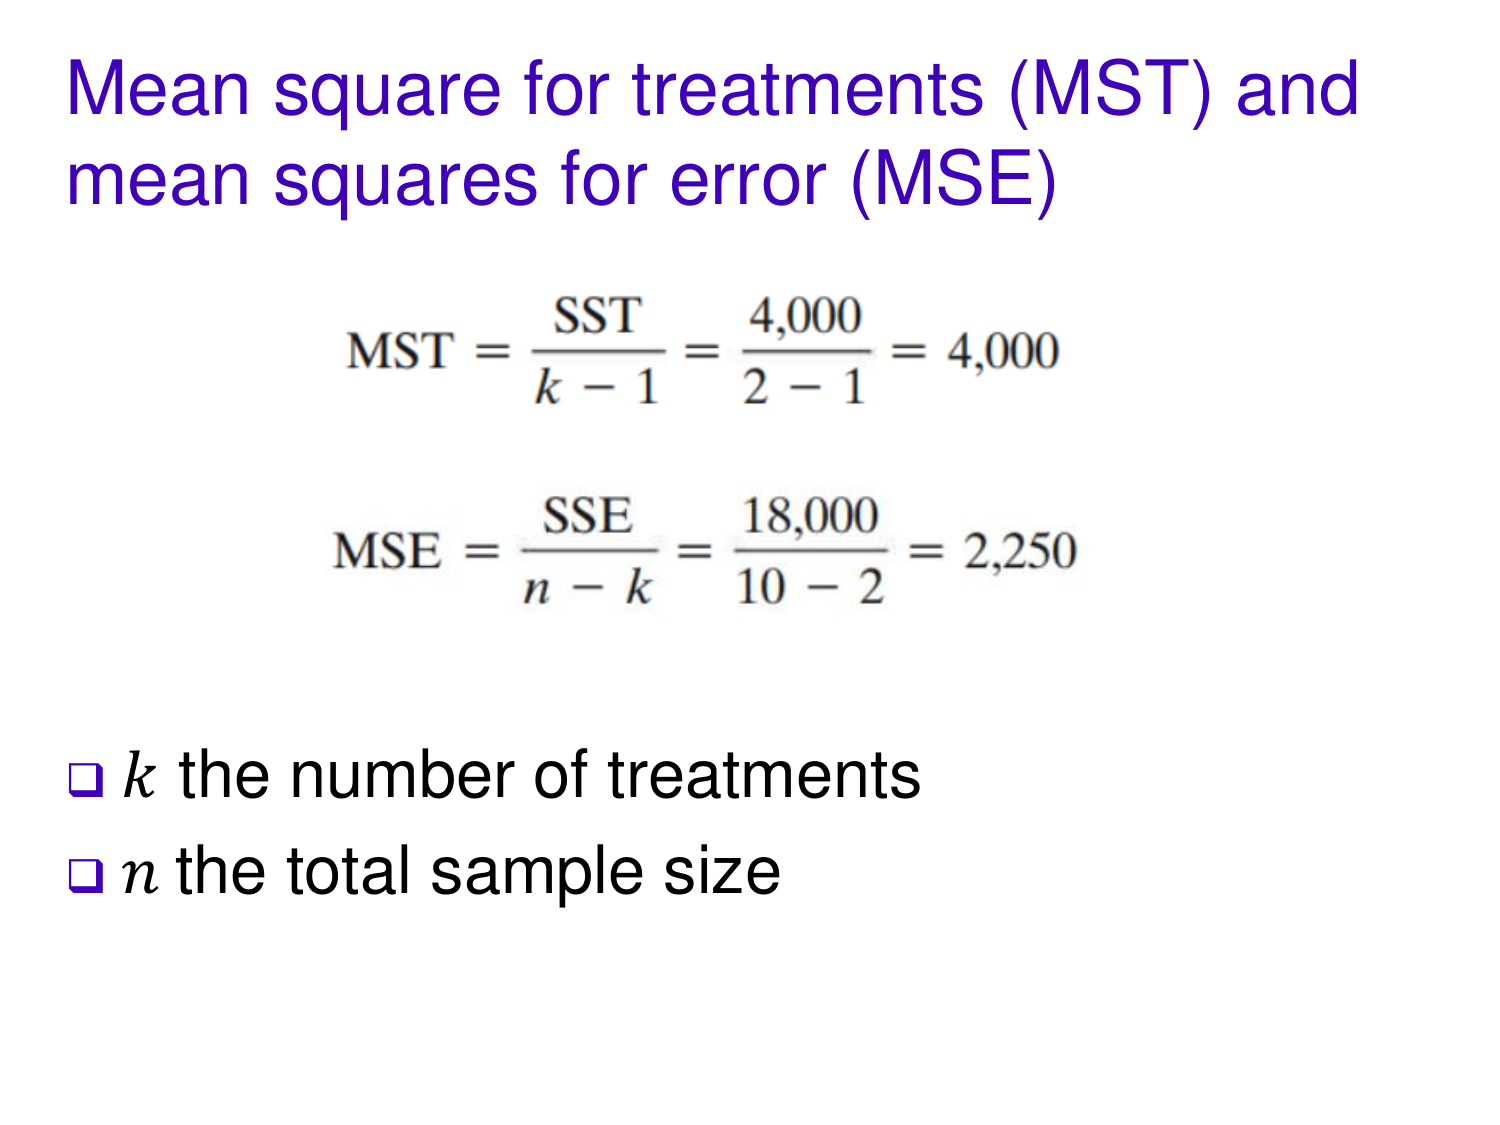
\includegraphics[width=0.78\textwidth]{assets/ch10-MST-MSE.png}
  \caption{Berekening van MST en MSE en de F-statistiek.}
\end{figure}

\frm{Gemiddelde kwadraten en F-statistiek}{F = \frac{MST}{MSE} = \frac{SST/(k-1)}{SSE/(n-k)}}{%
  $MST$ = gemiddelde kwadratensom behandelingen, $MSE$ = gemiddelde kwadratensom fout. $F \approx 1$ als $H_0$ waar is; $F \gg 1$ als minstens één behandelingsgemiddelde afwijkt.}

\begin{figure}[h!]
  \centering
  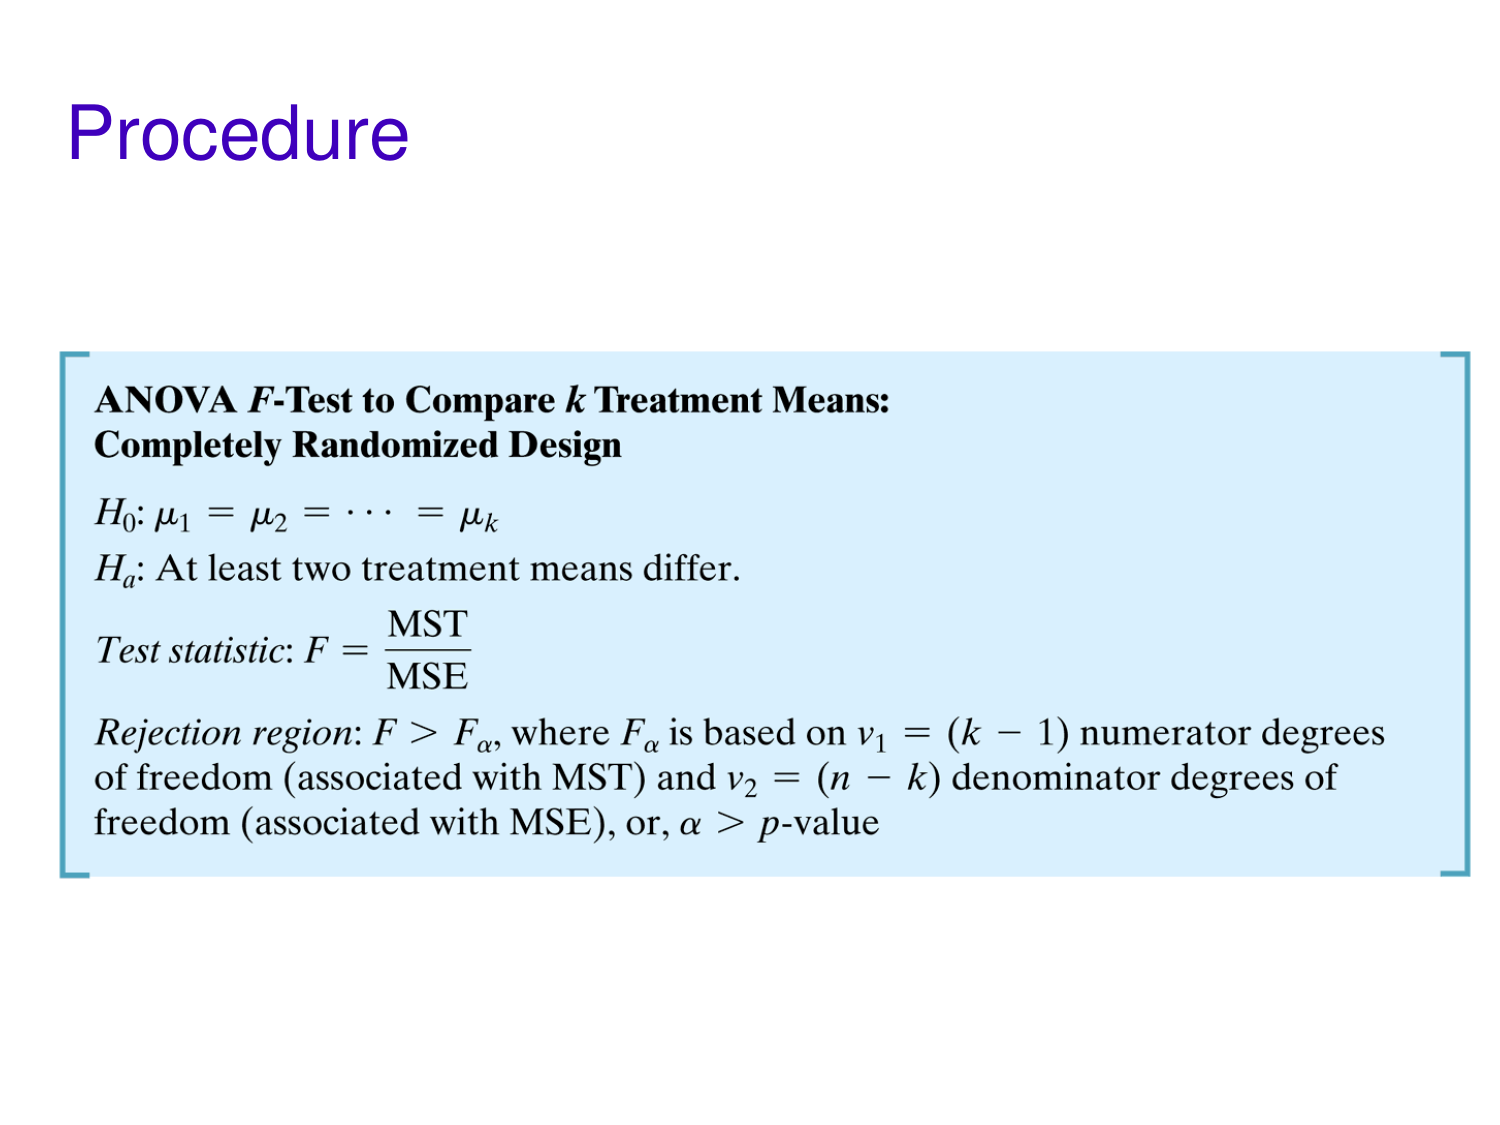
\includegraphics[width=0.78\textwidth]{assets/ch10-anova-procedure.png}
  \caption{Stappenplan voor de ANOVA F-toets.}
\end{figure}

\begin{figure}[h!]
  \centering
  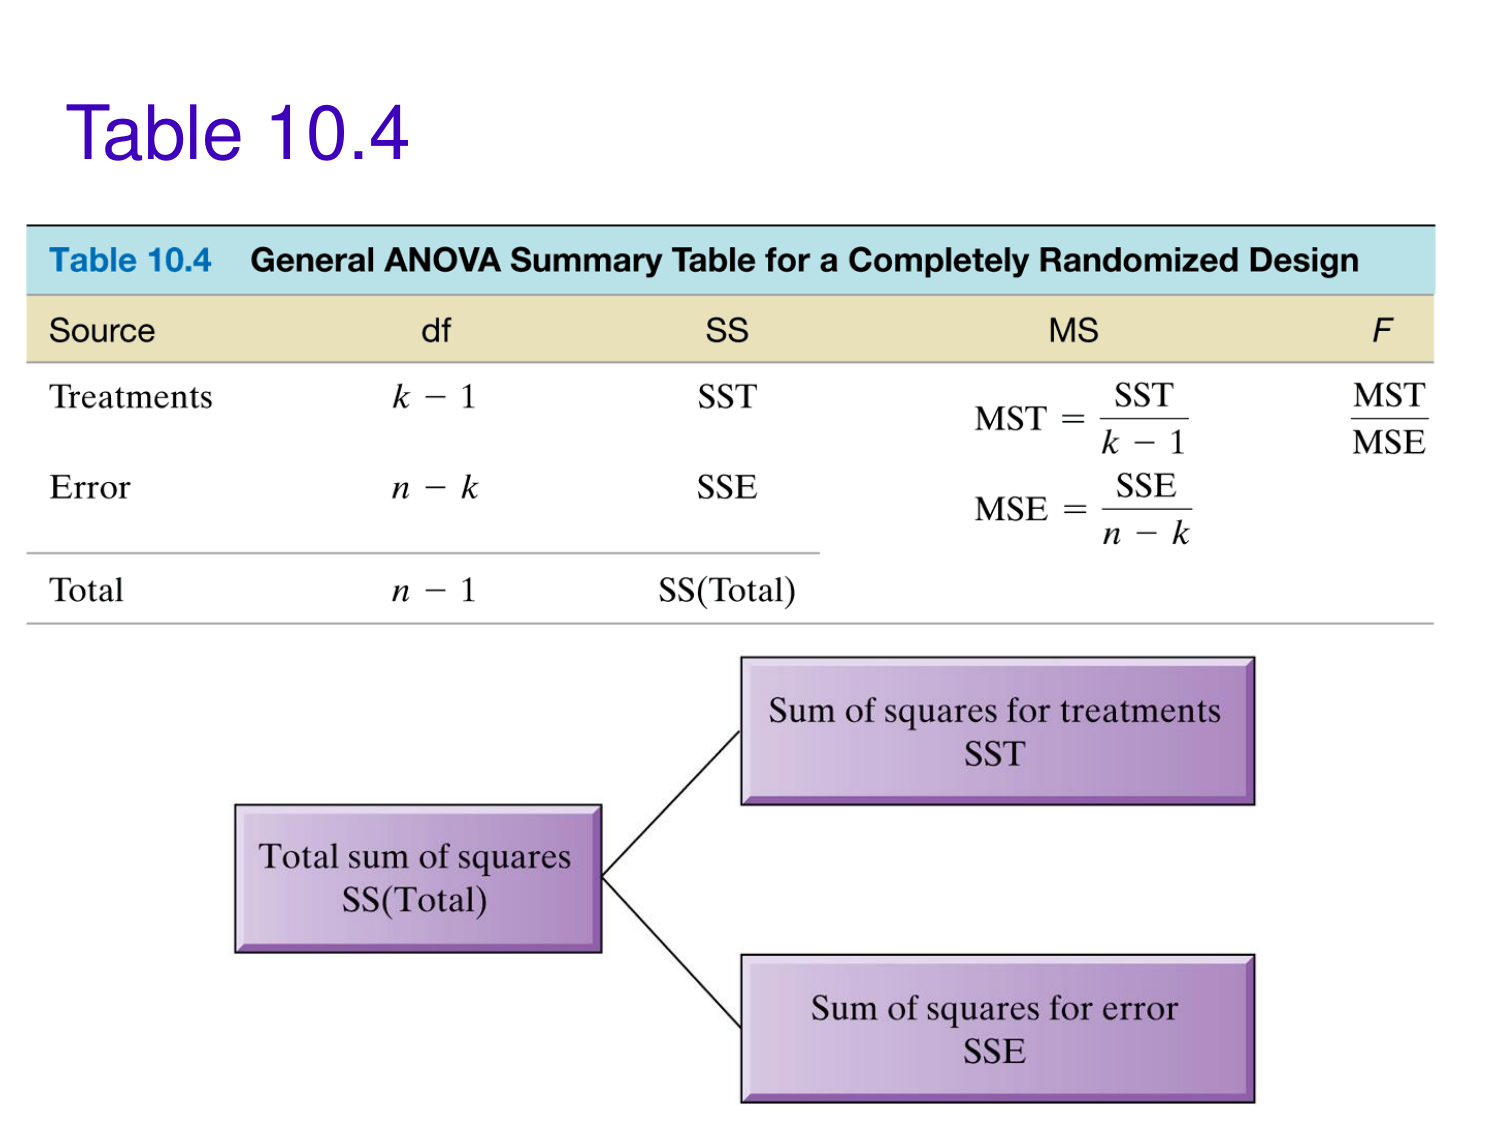
\includegraphics[width=0.72\textwidth]{assets/ch10-anova-tabel.png}
  \caption{ANOVA-tabel met SS, df, MS en F-statistiek.}
\end{figure}

\begin{examenbox}
\textbf{Aannames van ANOVA:}
\begin{enumerate}
  \item Steekproeven worden random en onafhankelijk getrokken uit elke behandelingsgroep.
  \item De responsvariabele is normaal verdeeld binnen elke groep.
  \item Alle behandelingsgroepen hebben \textbf{gelijke varianties} (controleer met boxplots).
\end{enumerate}
ANOVA is robuust voor afwijkingen van normaliteit, maar \emph{niet} robuust voor ongelijke varianties. Gebruik gelijke steekproefgrootten om dit te compenseren.
\end{examenbox}

\begin{conceptbox}{Verband met de $t$-toets}
Als er slechts 2 behandelingen zijn ($k=2$), is $F = t^2$ en zijn de ANOVA F-toets en de twee-steekproef $t$-toets equivalent. Bij meer dan 2 groepen heeft de F-toets een duidelijk voordeel: één toets voor alle groepen tegelijk.
\end{conceptbox}


\begin{voorbeeld}[Voorbeeld: golfbalmerken (ANOVA)]
4 merken golfballen, 10 ballen elk ($n=40$, $k=4$). Gemeten afstand in meter.
Stel: $SST=3855{,}0$, $SSE=7627{,}6$. Dan:
$$MST = \frac{3855{,}0}{3} = 1285{,}0 \qquad MSE = \frac{7627{,}6}{36} = 211{,}9 \qquad F = \frac{1285{,}0}{211{,}9} = 6{,}06$$
$F_{0{,}10; 3; 36} = 2{,}25$. $F = 6{,}06 > 2{,}25$ $\Rightarrow$ verwerp $H_0$. Minstens één merk verschilt.
\end{voorbeeld}

\begin{pyblock}
import numpy as np
from scipy import stats as sts
import pandas as pd

# Methode 1: scipy (meest direct)
merkA = [264, 261, 267, 272, 258, 263, 260, 265, 273, 257]
merkB = [268, 275, 260, 265, 270, 264, 271, 269, 263, 266]
merkC = [270, 273, 269, 274, 267, 271, 268, 272, 275, 266]
merkD = [267, 256, 262, 260, 265, 259, 264, 268, 254, 260]

F, p = sts.f_oneway(merkA, merkB, merkC, merkD)
print(f"F = {F:.3f}, p = {p:.4f}")

# Methode 2: volledige ANOVA-tabel (statsmodels)
import statsmodels.api as sm
from statsmodels.formula.api import ols

data = pd.DataFrame({
    'afstand': merkA + merkB + merkC + merkD,
    'merk': ['A']*10 + ['B']*10 + ['C']*10 + ['D']*10
})
model = ols('afstand ~ C(merk)', data=data).fit()
print(sm.stats.anova_lm(model))   # toont SS, df, MS, F, p
\end{pyblock}
\subsection{Meervoudige vergelijking van gemiddelden (Bonferroni)}

Nadat ANOVA aantoont dat \emph{minstens één} gemiddelde verschilt, wil je weten \emph{welke}. Het probleem: bij $c = \binom{k}{2}$ paargewijze vergelijkingen stijgt de kans op minstens één Type I fout (experiment-wise error rate).

\begin{figure}[h!]
  \centering
  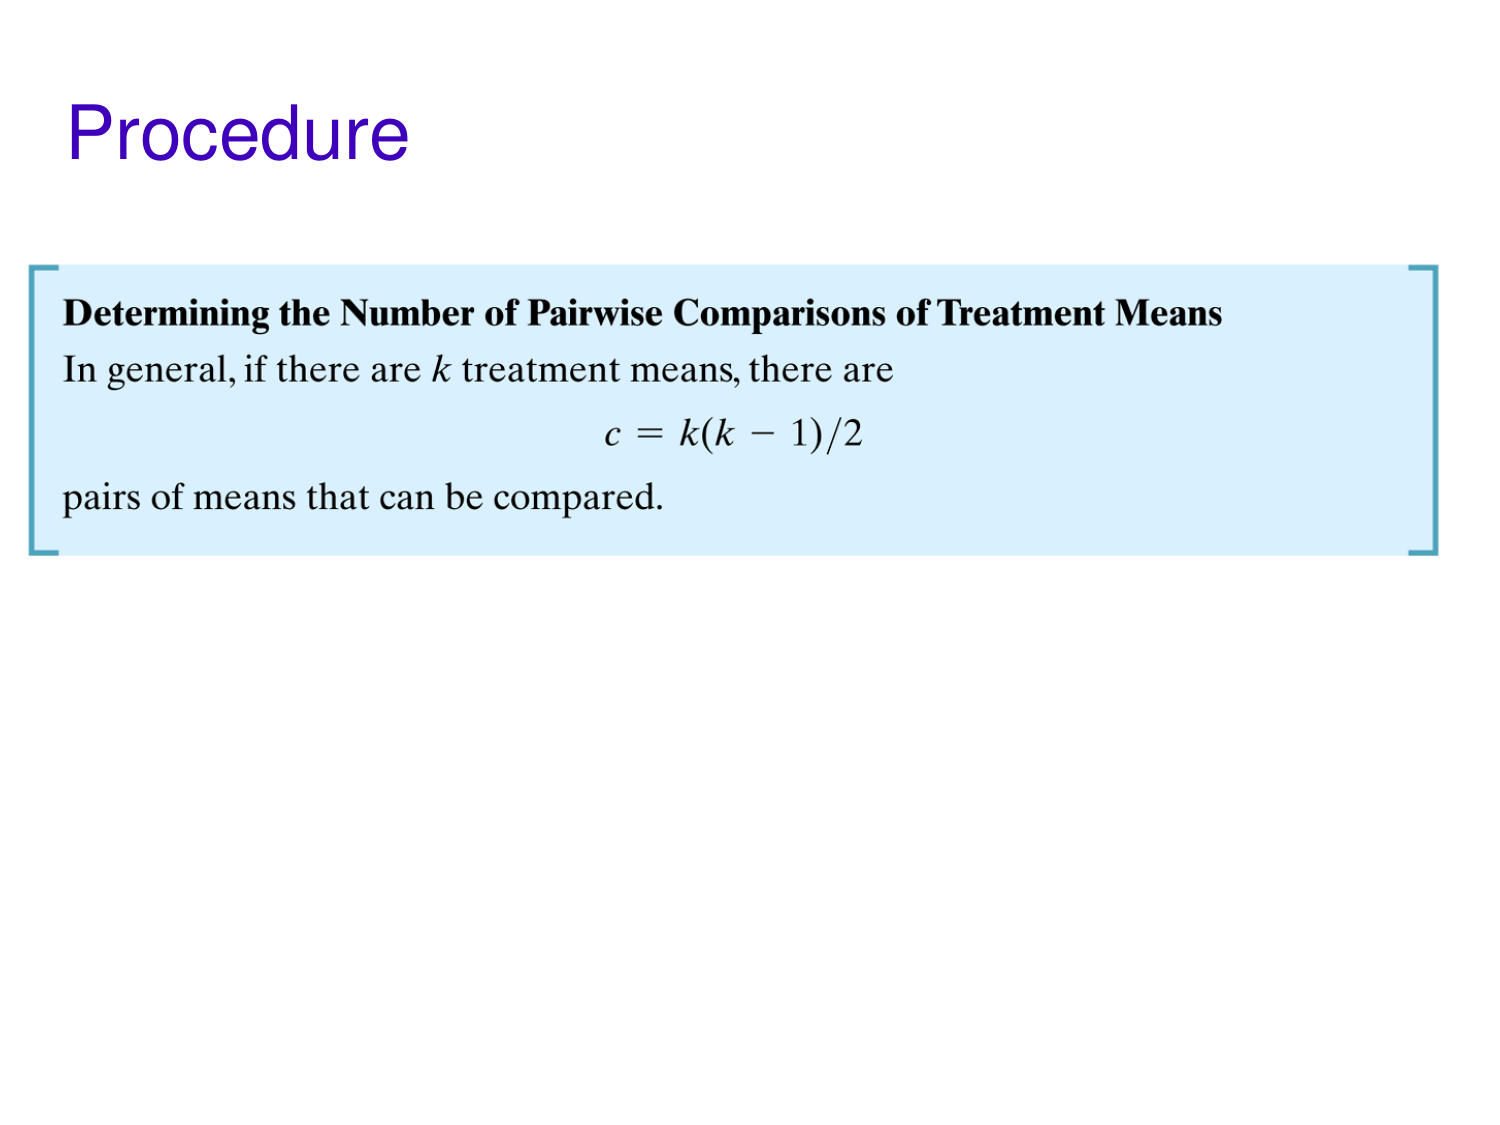
\includegraphics[width=0.72\textwidth]{assets/ch10-bonferroni-procedure.png}
  \caption{Bonferroni meervoudige vergelijkingsprocedure uit de slides.}
\end{figure}

\frm{Bonferroni BI voor $\mu_i - \mu_j$}{(\bar{x}_i - \bar{x}_j) \pm t_{\alpha/(2c),\,n-k} \cdot s_p\sqrt{\frac{1}{n_i} + \frac{1}{n_j}}}{%
  $c = \binom{k}{2}$ = aantal paargewijze vergelijkingen. $s_p = \sqrt{MSE}$ = gepoolde standaardafwijking. Door $\alpha/(2c)$ te gebruiken (Bonferroni-correctie) blijft de experiment-wise error rate $\leq \alpha$.}

\begin{conceptbox}{Experiment-wise foutenkans}
Als je $c$ vergelijkingen uitvoert, elk op niveau $\alpha$, dan is de kans op minstens één fout $\leq c\alpha$ (Bonferroni-ongelijkheid). Door elk afzonderlijk op niveau $\alpha/c$ te toetsen, houdt de totale foutenkans $\leq \alpha$.
\end{conceptbox}

% =============================================================================

\begin{pyblock}
import numpy as np
from scipy import stats as sts
import statsmodels.stats.multicomp as mc

# Bonferroni pairwise na ANOVA:
scores = merkA + merkB + merkC + merkD
groepen = ['A']*10 + ['B']*10 + ['C']*10 + ['D']*10

comp = mc.MultiComparison(scores, groepen)
result = comp.allpairtest(sts.ttest_ind, method='bonf')
print(result[0])                   # overzicht van alle paarsgewijze toetsen

# Handmatig Bonferroni CI voor mu_i - mu_j:
MSE = 211.9
sp = np.sqrt(MSE)
n_i, n_j = 10, 10
k, n = 4, 40
c = 6                              # aantal paren = k*(k-1)/2
alpha_bonf = 0.05 / (2*c)        # gecorrigeerd alpha
t_bonf = sts.t.ppf(1 - alpha_bonf, df=n-k)
diff = np.mean(merkC) - np.mean(merkA)
marge = t_bonf * sp * np.sqrt(1/n_i + 1/n_j)
print(f"CI merkC-merkA: ({diff-marge:.2f}, {diff+marge:.2f})")
\end{pyblock}
\section{Ch.\ 11 -- Enkelvoudige Lineaire Regressie}
% =============================================================================

\begin{conceptbox}{Wat is lineaire regressie?}
\textbf{Lineaire regressie} beschrijft het lineaire verband tussen een \emph{responsvariabele} $y$ en een \emph{verklarende variabele} $x$. Het model laat toe om $y$ te \emph{voorspellen} op basis van $x$ en te toetsen of er een significant lineair verband bestaat.

\medskip
\textbf{Kenmerk:} beide variabelen zijn kwantitatief. Bij slechts één verklarende variabele spreken we van \emph{enkelvoudige} lineaire regressie.
\end{conceptbox}

\subsection{Het probabilistisch model}

\begin{figure}[h!]
  \centering
  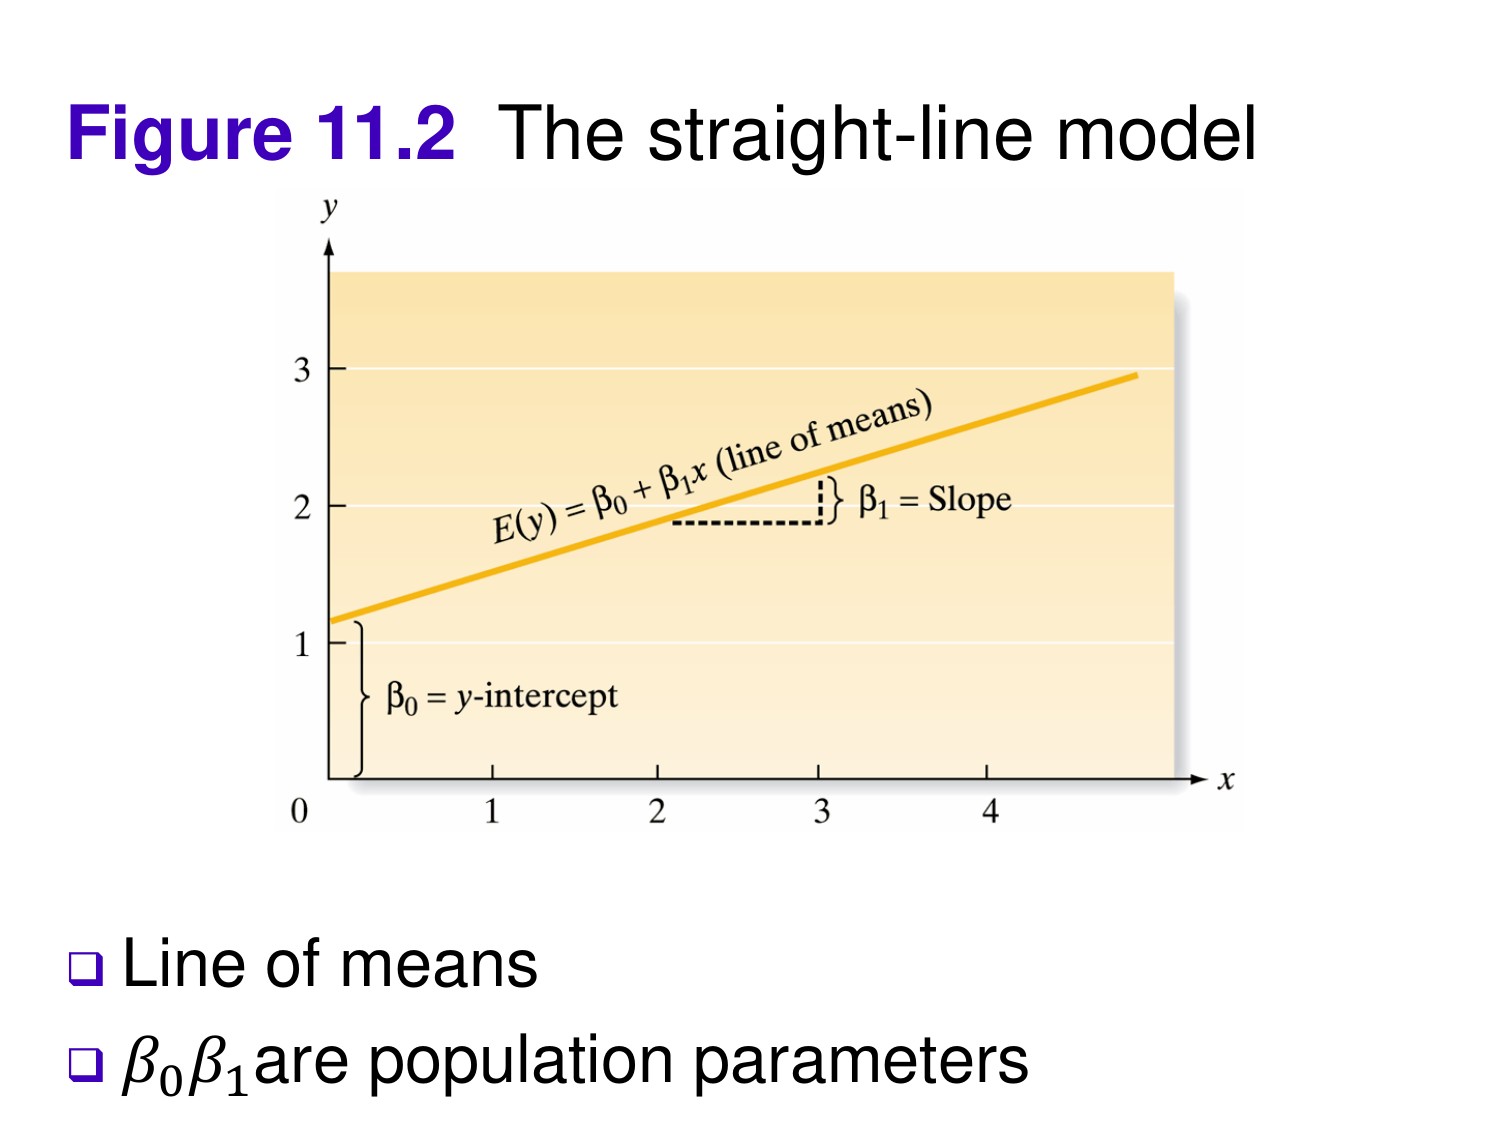
\includegraphics[width=0.72\textwidth]{assets/ch11-regressielijn-model.png}
  \caption{Het rechtelijnmodel: $E(y) = \beta_0 + \beta_1 x$ is de gemiddeldenlijn; $\varepsilon$ is de willekeurige fout.}
\end{figure}

\frm{Enkelvoudig lineair model}{y = \beta_0 + \beta_1 x + \varepsilon}{%
  $\beta_0$ = y-snijpunt (populatieparameter), $\beta_1$ = helling (populatieparameter), $\varepsilon$ = willekeurige fout met $E(\varepsilon)=0$.
  Het \emph{deterministische} deel $\beta_0 + \beta_1 x$ geeft de gemiddelde respons; $\varepsilon$ verklaart de resterende variatie.}

\sym{beta0}{Y-snijpunt van de regressielijn (populatie)}{--}
\sym{beta1}{Helling van de regressielijn (populatie)}{--}

\subsection{De kleinste-kwadratenmethode}

\begin{theorieblok}{Hoe vind je de beste rechte lijn?}
De \textbf{kleinste-kwadratenlijn} minimaliseert de som van gekwadrateerde residuen:
\[
  SSE = \sum_{i=1}^n (y_i - \hat{y}_i)^2 = \sum_{i=1}^n (y_i - \hat{\beta}_0 - \hat{\beta}_1 x_i)^2
\]
Er bestaat precies één lijn die SSE minimaliseert.
\end{theorieblok}

\begin{figure}[h!]
  \centering
  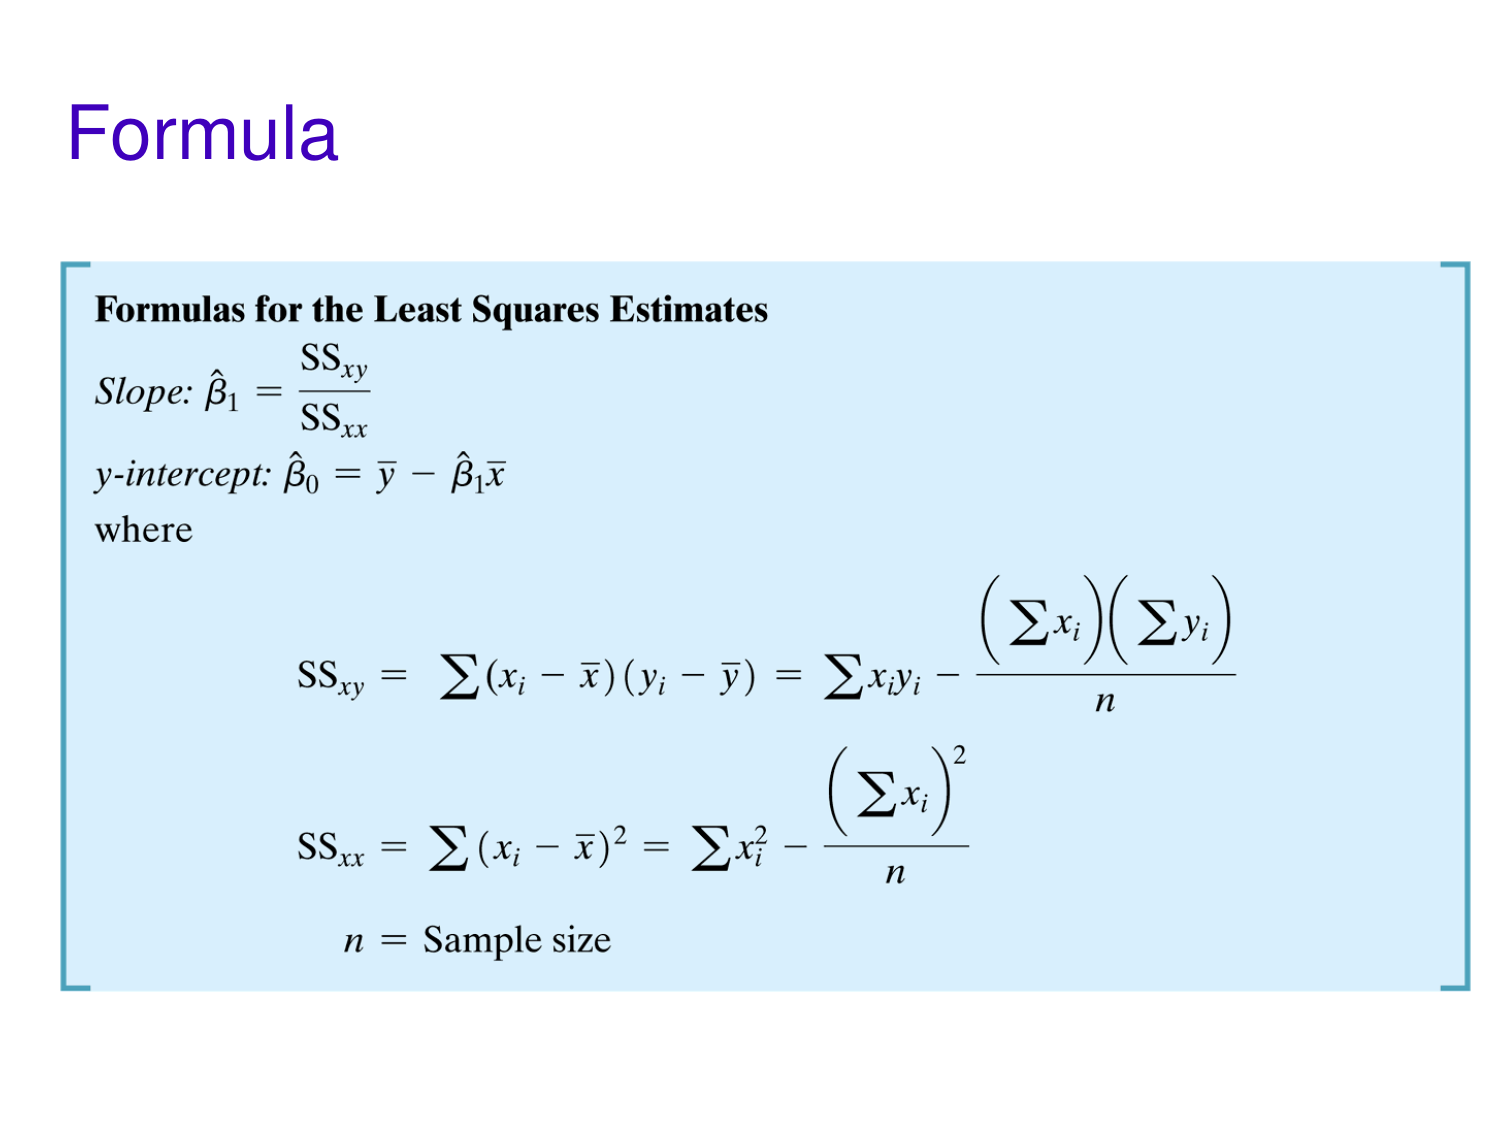
\includegraphics[width=0.72\textwidth]{assets/ch11-kleinste-kwadraten-formule.png}
  \caption{Formules voor de kleinste-kwadratensckatters $\hat{\beta}_0$ en $\hat{\beta}_1$ (uit de slides).}
\end{figure}

\frm{Kleinste-kwadratenschatters}{%
  \hat{\beta}_1 = \frac{SS_{xy}}{SS_{xx}}, \quad
  \hat{\beta}_0 = \bar{y} - \hat{\beta}_1\,\bar{x}}{%
  $SS_{xy} = \sum x_i y_i - n\bar{x}\bar{y}$, $SS_{xx} = \sum x_i^2 - n\bar{x}^2$.
  Interpretatie: $\hat{\beta}_1$ = verandering in gemiddelde $y$ per eenheid toename in $x$; $\hat{\beta}_0$ alleen zinvol als $x=0$ in het bereik van de data ligt.}

\begin{figure}[h!]
  \centering
  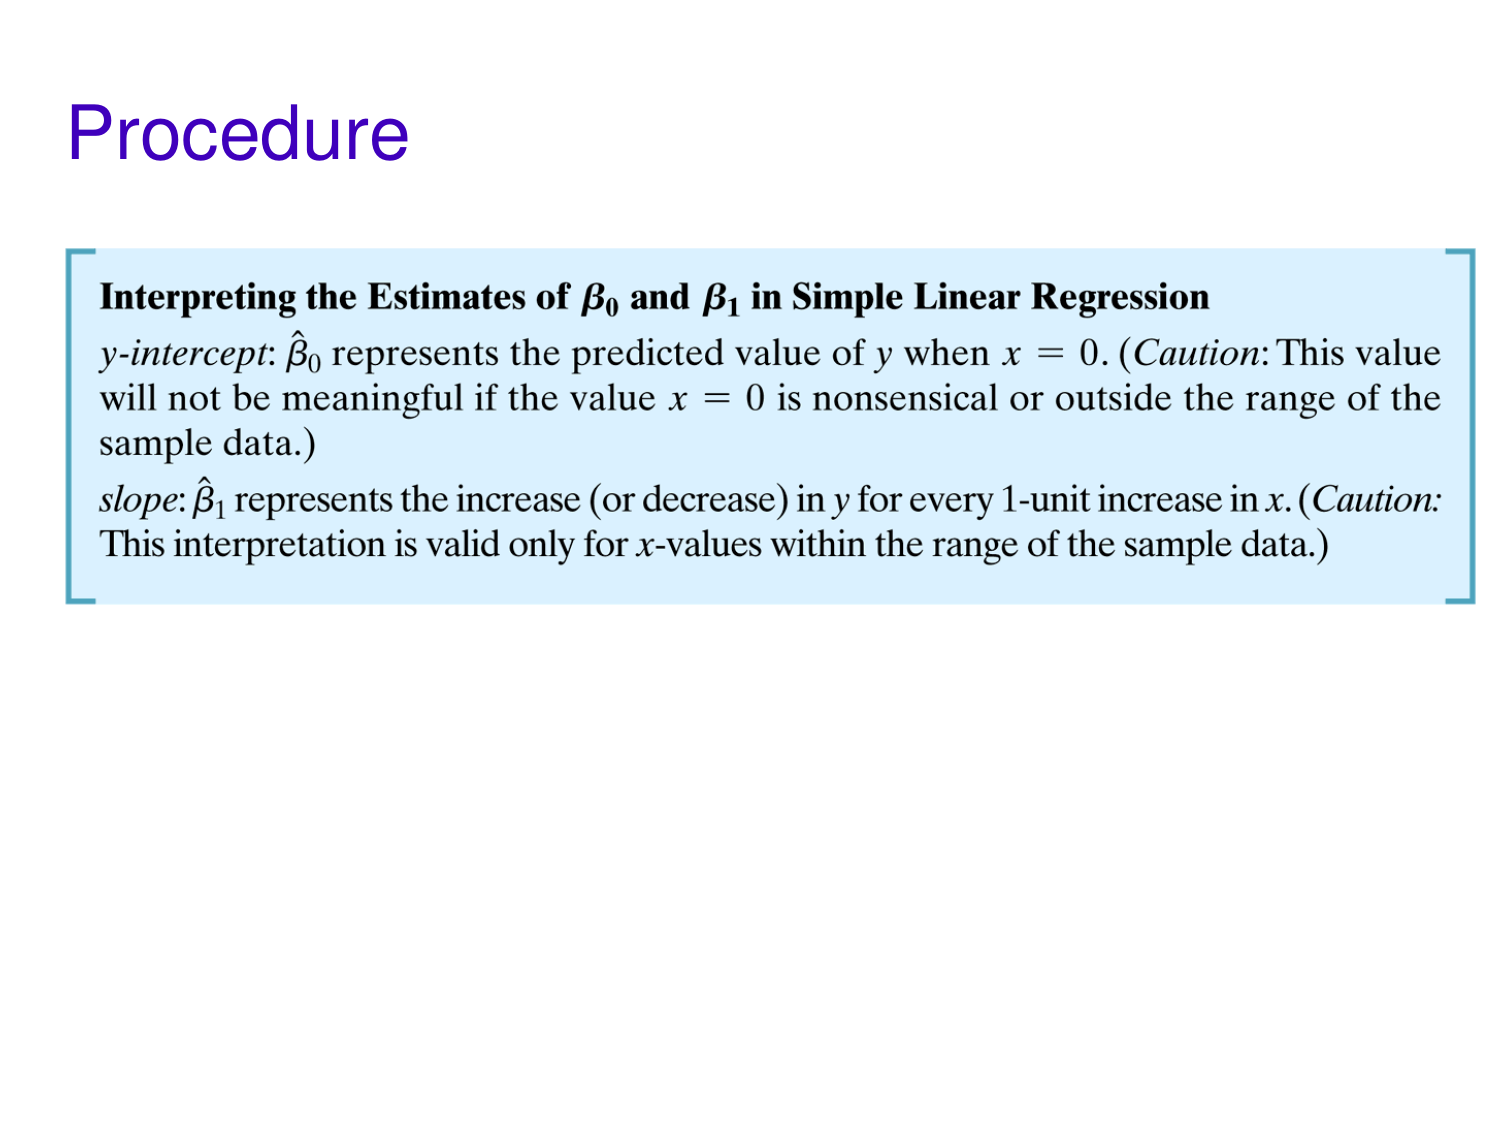
\includegraphics[width=0.72\textwidth]{assets/ch11-interpretatie-parameters.png}
  \caption{Interpretatie van $\hat{\beta}_0$ en $\hat{\beta}_1$ (enkel geldig binnen het bereik van de data).}
\end{figure}


\begin{voorbeeld}[Voorbeeld: drug-reactietijd (regressie)]
5 ratten: $x$ = \% drug, $y$ = reactietijd. Data: $(1,1{,}0)$, $(2,1{,}8)$, $(3,2{,}7)$, $(4,3{,}2)$, $(5,3{,}9)$.

$SS_{xx} = 10$, $SS_{xy} = 7$. Dan: $\hat{\beta}_1 = 7/10 = 0{,}7$ en $\hat{\beta}_0 = 2{,}72 - 0{,}7 \cdot 3 = 0{,}62$.

Model: $\hat{y} = -0{,}1 + 0{,}7x$ (interpretatie: per 1\% extra drug stijgt de reactietijd met 0{,}7 sec).
\end{voorbeeld}

\begin{pyblock}
import numpy as np
from scipy import stats as sts

x = np.array([1, 2, 3, 4, 5])    # verklarende variabele
y = np.array([1.0, 1.8, 2.7, 3.2, 3.9])  # responsvariabele

# Volledige resultaten in 1 functie:
slope, intercept, r, p, se = sts.linregress(x, y)
print(f"y = {intercept:.3f} + {slope:.3f}*x")
print(f"r = {r:.3f},  r^2 = {r**2:.3f}")
print(f"p-waarde helling beta1: {p:.4f}")
print(f"SE van helling: {se:.4f}")

# Voorspelling bij x=3:
y_hat = intercept + slope * 3
print(f"Voorspelling bij x=3: {y_hat:.3f}")

# Residuen:
y_pred = intercept + slope * x
residuals = y - y_pred
SSE = np.sum(residuals**2)
s2 = SSE / (len(x) - 2)           # MSE
print(f"s^2 = {s2:.4f},  s = {np.sqrt(s2):.4f}")
\end{pyblock}
\subsection{Aannames van het model}

\begin{figure}[h!]
  \centering
  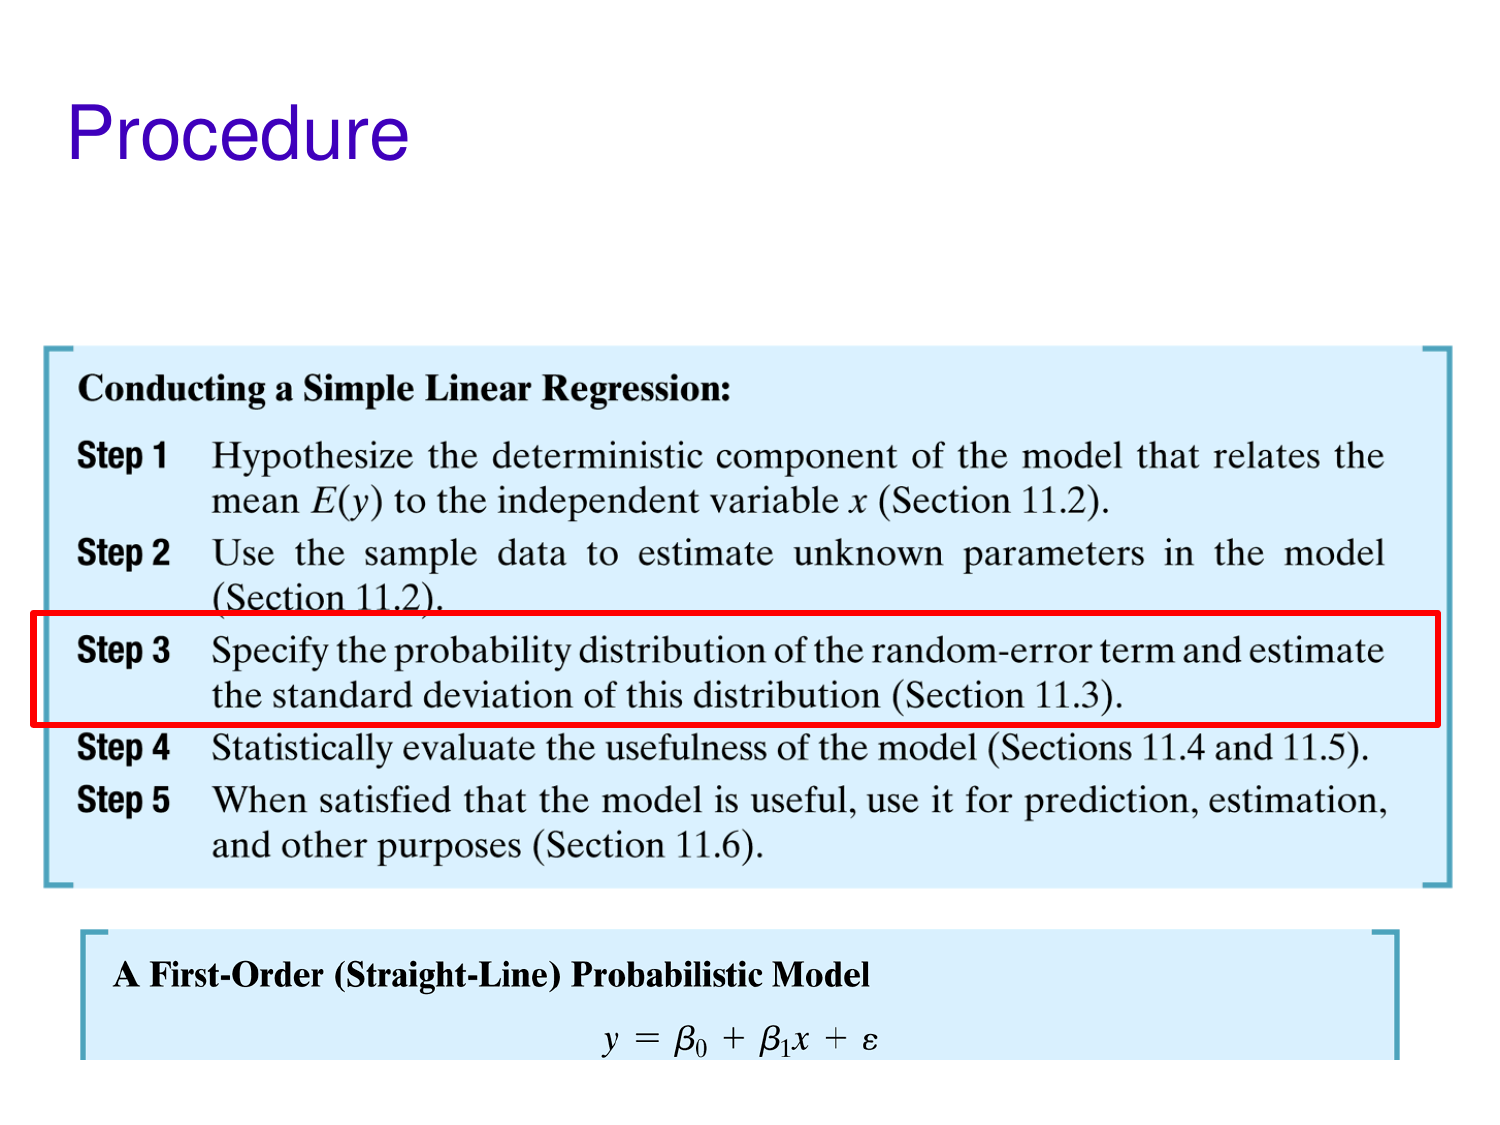
\includegraphics[width=0.72\textwidth]{assets/ch11-modelaannames.png}
  \caption{Aannames voor het lineaire regressiemodel: $\varepsilon \sim N(0, \sigma^2)$, onafhankelijk en homoscedastisch.}
\end{figure}

\frm{Schatting van $\sigma^2$ (MSE)}{s^2 = \frac{SSE}{n-2}}{%
  $SSE = SS_{yy} - \hat{\beta}_1\,SS_{xy}$, $SS_{yy} = \sum y_i^2 - n\bar{y}^2$.
  Vrijheidsgraden $= n-2$ (twee parameters $\hat{\beta}_0$ en $\hat{\beta}_1$ geschat). De meeste datapunten liggen binnen $2s$ van de regressielijn.}

\subsection{Toets en BI voor de helling $\beta_1$}

\begin{conceptbox}{Waarom de helling toetsen?}
Als $\beta_1 = 0$, verandert $E(y)$ niet met $x$ -- er is geen lineaire relatie. De toets $H_0: \beta_1 = 0$ vs.\ $H_a: \beta_1 \neq 0$ bepaalt of $x$ bijdraagt aan de voorspelling van $y$.
\end{conceptbox}

\frm{T-toets voor de helling $\beta_1$}{t = \frac{\hat{\beta}_1}{s/\sqrt{SS_{xx}}}}{%
  $t$-verdeling met $\nu = n-2$ vrijheidsgraden. Verwerp $H_0: \beta_1 = 0$ als $|t| > t_{\alpha/2, n-2}$.}

\begin{figure}[h!]
  \centering
  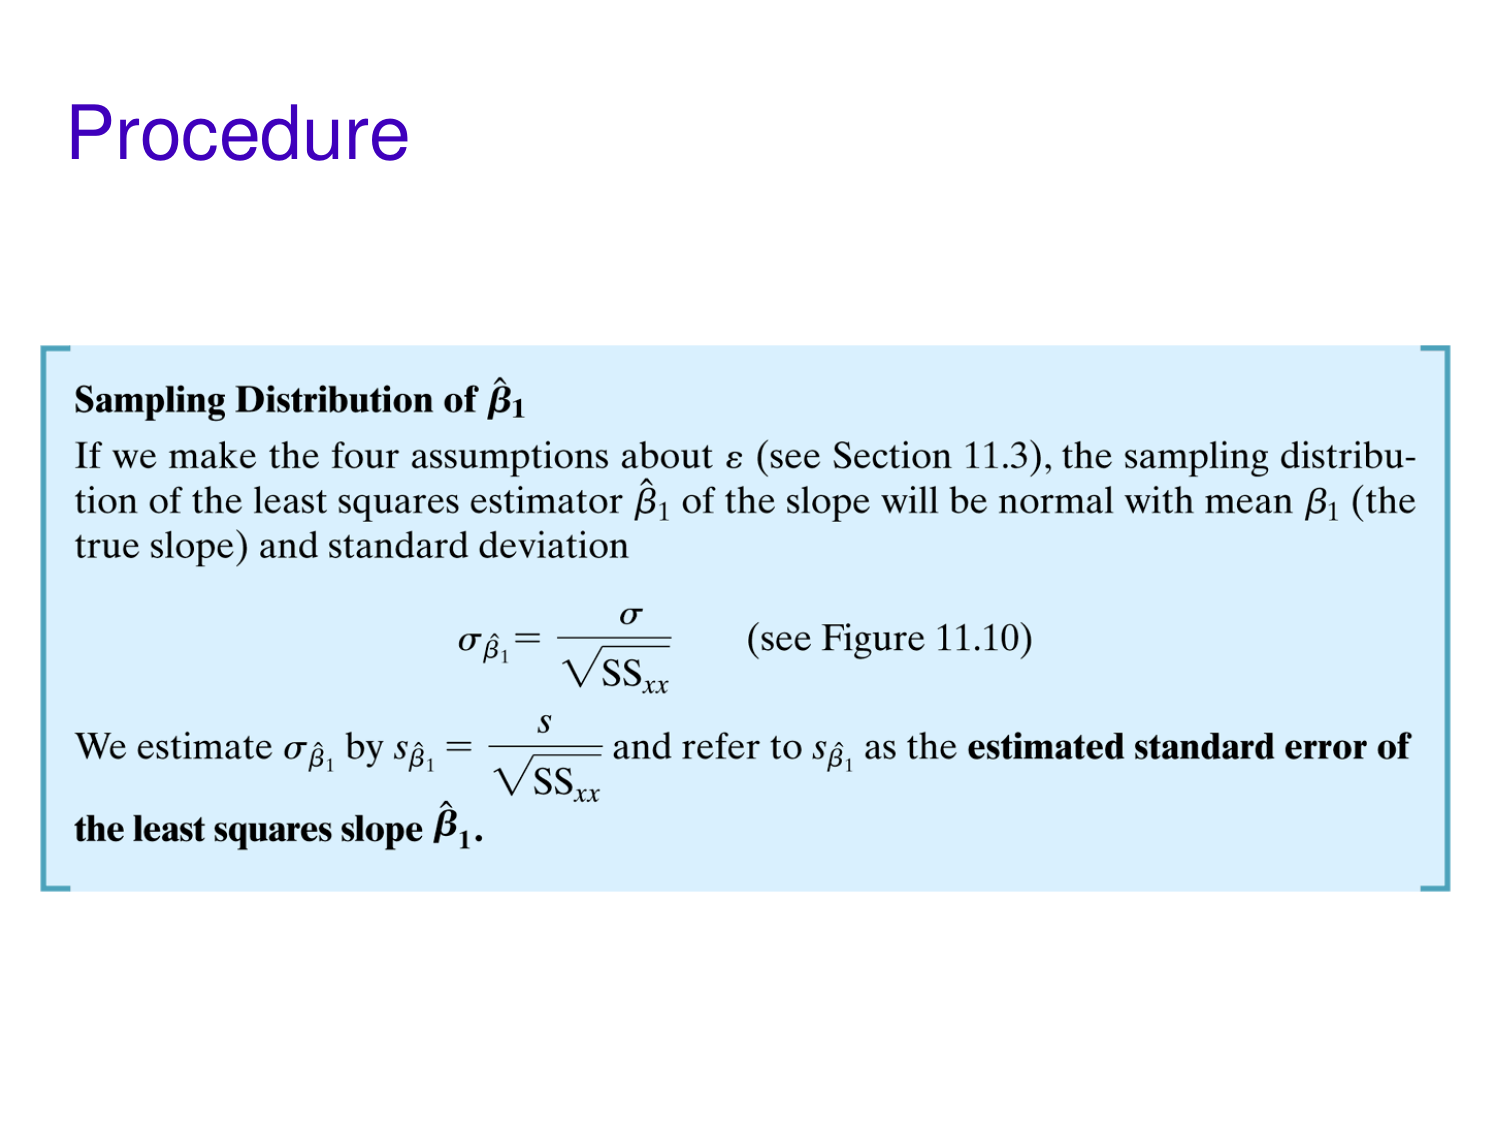
\includegraphics[width=0.78\textwidth]{assets/ch11-t-toets-helling.png}
  \caption{Toets voor de helling: verwerp $H_0$ als $|t|$ het kritieke gebied overschrijdt.}
\end{figure}

\frm{Betrouwbaarheidsinterval voor $\beta_1$}{\hat{\beta}_1 \pm t_{\alpha/2,\,n-2} \cdot \frac{s}{\sqrt{SS_{xx}}}}{%
  Als het BI nul niet bevat, is er significant bewijs voor een lineair verband. Vergroot $SS_{xx}$ (meer data of groter $x$-bereik) om het interval te verkleinen.}

\begin{figure}[h!]
  \centering
  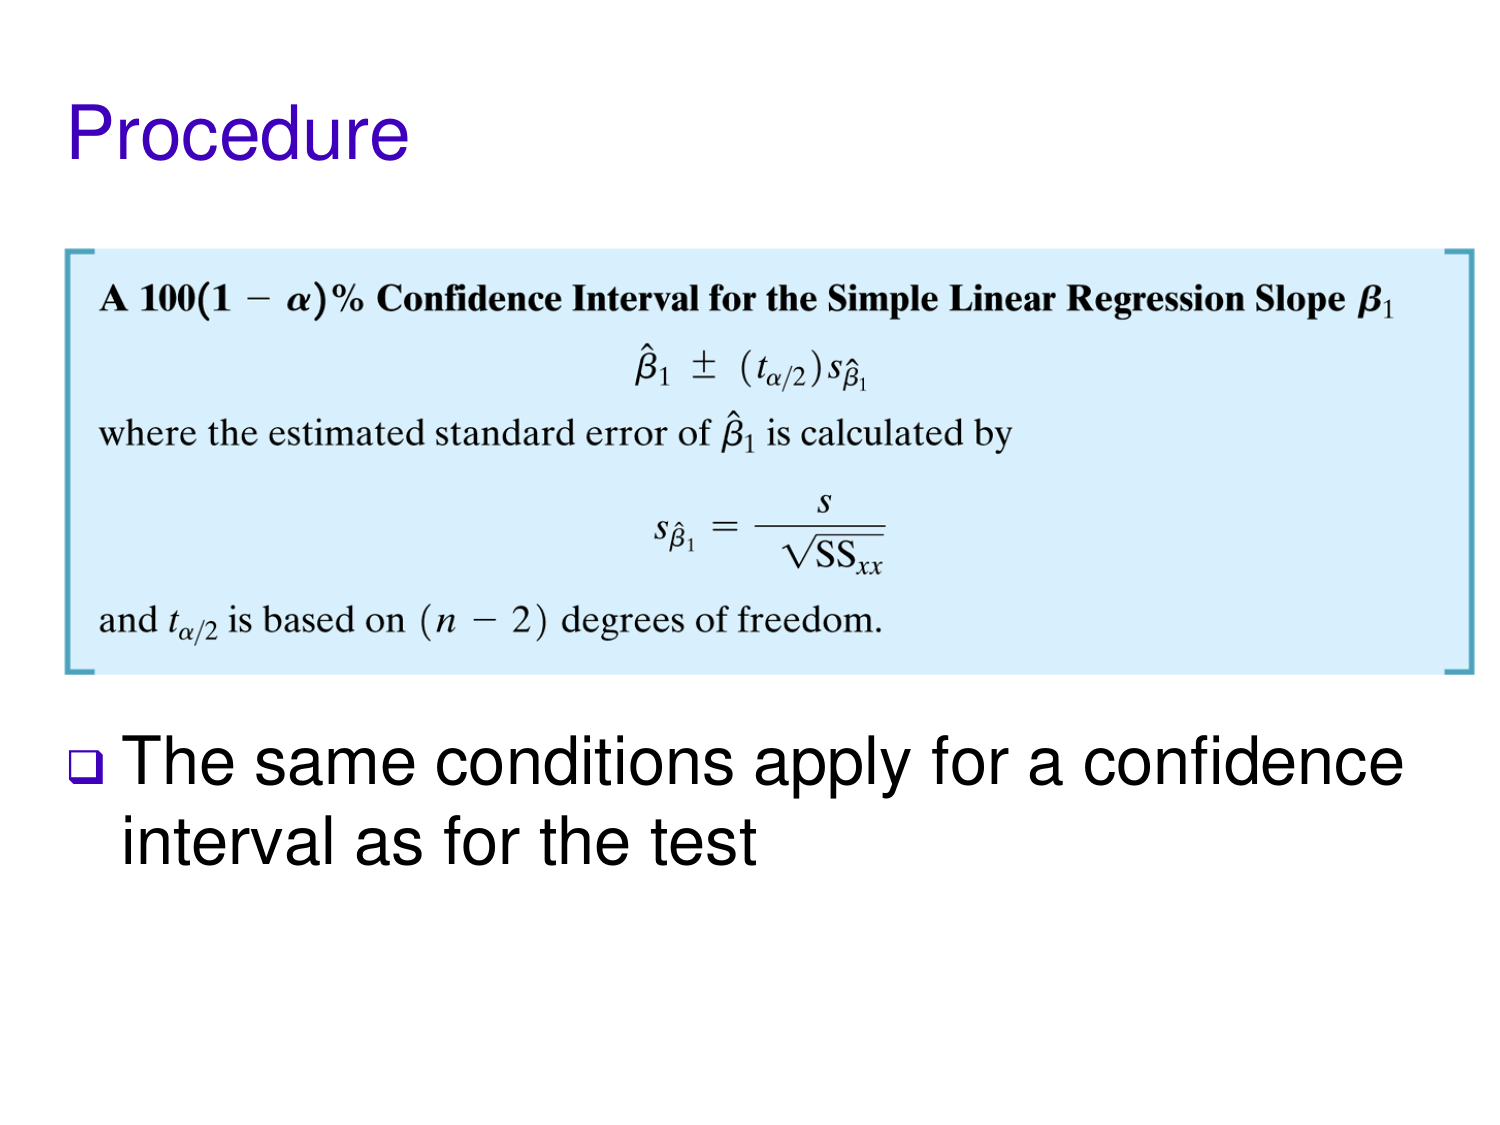
\includegraphics[width=0.72\textwidth]{assets/ch11-CI-helling.png}
  \caption{Procedure voor het betrouwbaarheidsinterval van de helling.}
\end{figure}


\begin{pyblock}
import numpy as np
import statsmodels.formula.api as smf
import pandas as pd

df = pd.DataFrame({'x': [1,2,3,4,5], 'y': [1.0,1.8,2.7,3.2,3.9]})
model = smf.ols('y ~ x', data=df).fit()

# Volledige samenvatting (toetsing beta1, CI, R^2...):
print(model.summary())

# Specifieke waarden:
print(model.params)               # [intercept, slope]
print(model.conf_int(alpha=0.05)) # 95% CI voor beta0 en beta1
print(model.pvalues)              # p-waarden
print(model.rsquared)             # R^2
print(model.mse_resid)            # s^2 = MSE

# Voorspelling:
x_new = pd.DataFrame({'x': [3.5]})
print(model.predict(x_new))       # y_hat bij x=3.5
\end{pyblock}
\subsection{Correlatie- en determinatiecoëfficiënt}

\begin{figure}[h!]
  \centering
  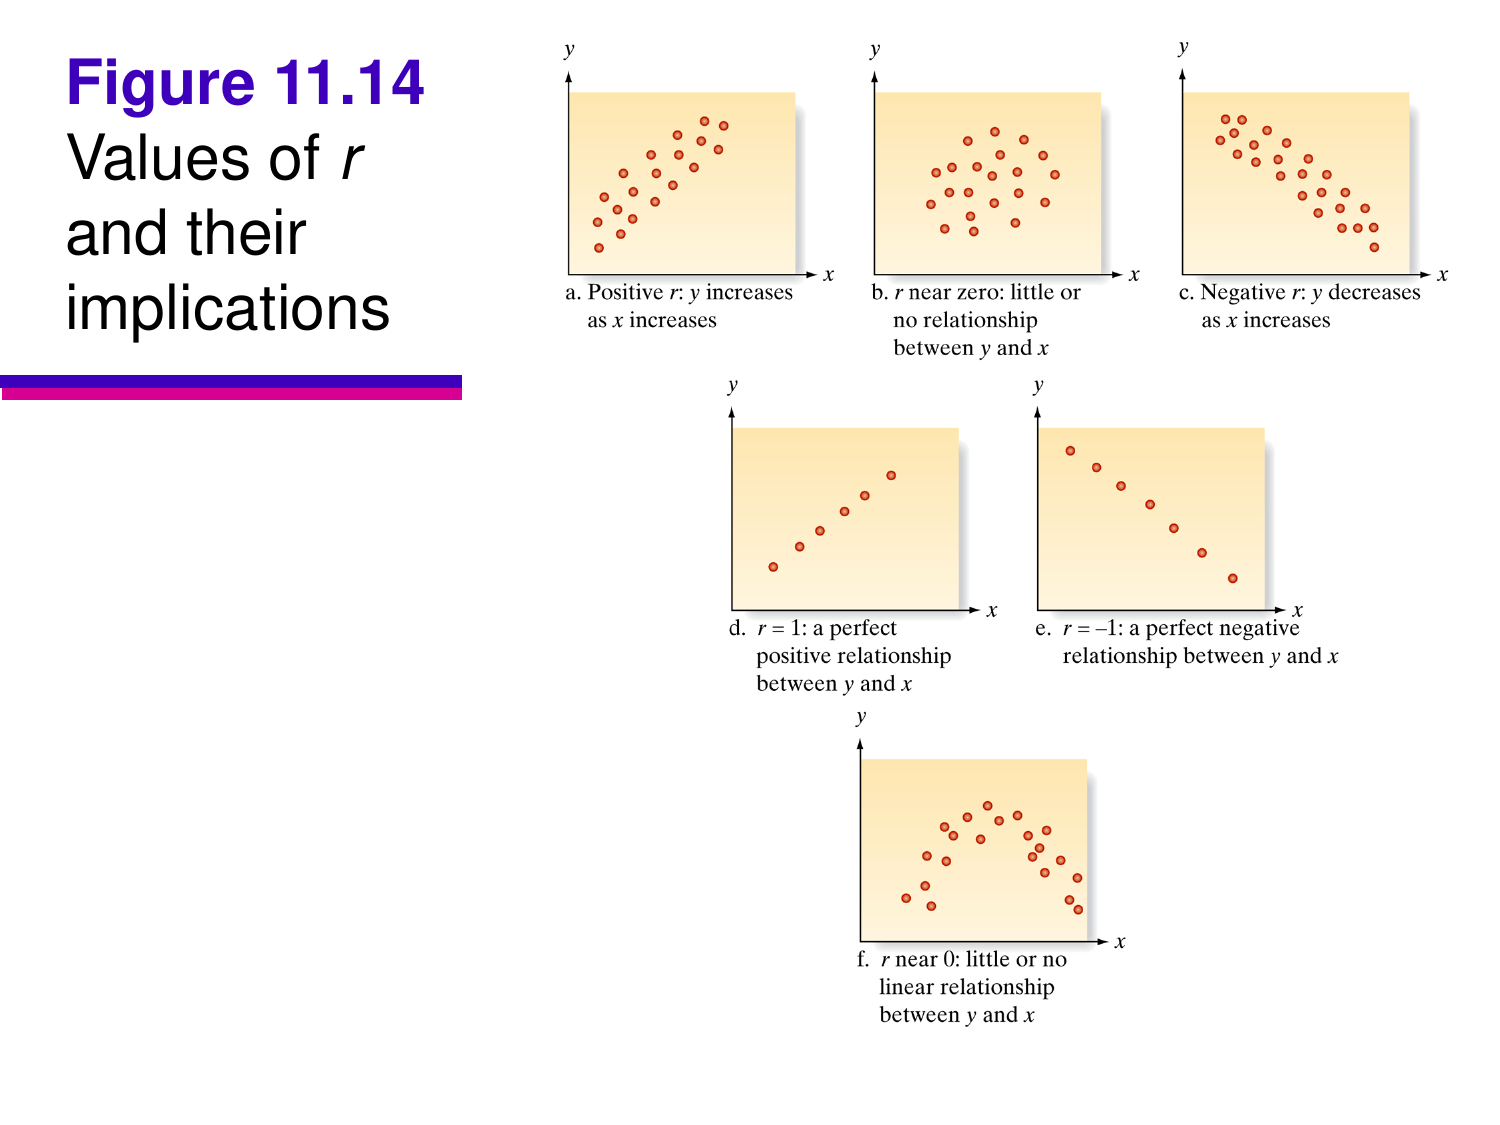
\includegraphics[width=0.72\textwidth]{assets/ch11-correlatiecoefficient.png}
  \caption{Correlatiecoëfficiënt $r$: variatie van $-1$ (perfect negatief) tot $+1$ (perfect positief).}
\end{figure}

\frm{Pearson correlatiecoëfficiënt $r$}{r = \frac{SS_{xy}}{\sqrt{SS_{xx}\,SS_{yy}}}}{%
  $r \in [-1, 1]$. $r = 0$ betekent geen lineair verband; $r = \pm1$ betekent alle punten op de rechte lijn. Let op: correlatie impliceert \emph{geen} causaliteit!
  $r$ heeft hetzelfde teken als $\hat{\beta}_1$.}

\sym{r}{Pearson correlatiecoëfficiënt}{--}

\begin{figure}[h!]
  \centering
  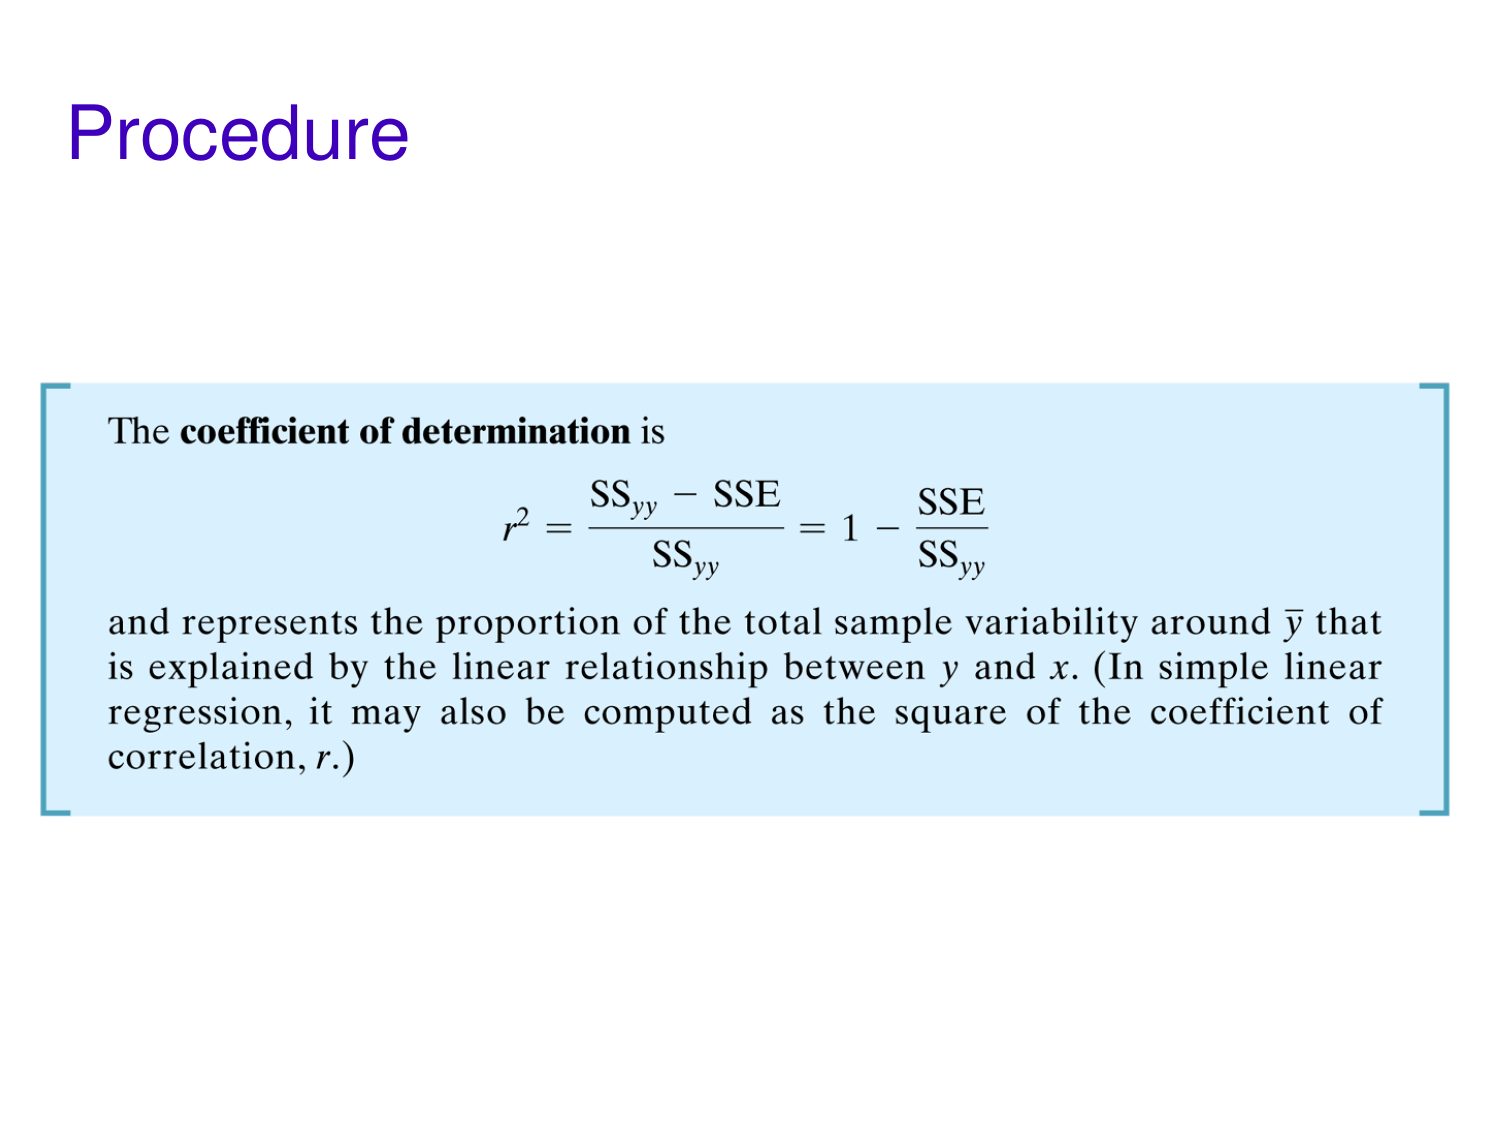
\includegraphics[width=0.72\textwidth]{assets/ch11-determinatiecoefficient.png}
  \caption{Determinatiecoëfficiënt $r^2$: het aandeel van de variatie in $y$ verklaard door het model.}
\end{figure}

\frm{Determinatiecoëfficiënt $r^2$}{r^2 = 1 - \frac{SSE}{SS_{yy}} = \frac{SS_{yy} - SSE}{SS_{yy}}}{%
  $r^2 \in [0, 1]$. $r^2 = 0{,}82$ betekent: 82\% van de steekproefvariatie in $y$ wordt verklaard door het rechtelijnmodel met $x$.
  In enkelvoudige regressie: $r^2 = r \cdot r$ (het kwadraat van de correlatiecoëfficiënt).}

\sym{r2}{Determinatiecoëfficiënt (verklaarde variantie)}{--}


\begin{pyblock}
import numpy as np
from scipy import stats as sts

x = np.array([1, 2, 3, 4, 5])
y = np.array([1.0, 1.8, 2.7, 3.2, 3.9])

# Pearson correlatiecoefficient:
r, p_waarde = sts.pearsonr(x, y)
print(f"r = {r:.3f},  r^2 = {r**2:.3f}")
print(f"p-waarde (H0: rho=0): {p_waarde:.4f}")

# r^2 uit linregress:
slope, intercept, r_val, p, se = sts.linregress(x, y)
print(f"r^2 = {r_val**2:.3f}")   # verklaarde variantie

# Interpretatie:
if abs(r) > 0.9:
    print("Sterk lineair verband")
elif abs(r) > 0.7:
    print("Matig lineair verband")
else:
    print("Zwak lineair verband")
\end{pyblock}


\begin{examenbox}
\textbf{Volgorde bij regressieanalyse:}
\begin{enumerate}
  \item Maak een scatterplot -- is een rechte lijn een goed model?
  \item Bereken $\hat{\beta}_0$, $\hat{\beta}_1$ via de kleinste-kwadratenmethode.
  \item Schat $\sigma^2 = s^2 = SSE/(n-2)$.
  \item Toets $H_0: \beta_1 = 0$ (of bereken het BI voor $\beta_1$).
  \item Bereken $r$ en $r^2$ voor de sterkte en verklaarde variatie.
\end{enumerate}
\textbf{Pas op:} extrapoleer nooit buiten het bereik van de $x$-waarden!
\end{examenbox}


\newpage
\section{Python Referentie -- Statistiek}
\label{sec:python}

\begin{conceptbox}{Basisimports -- altijd bovenaan je notebook}
\begin{verbatim}
import numpy as np
from scipy import stats as sts
import pandas as pd
import statsmodels.formula.api as smf
import statsmodels.api as sm
import matplotlib.pyplot as plt
\end{verbatim}
\end{conceptbox}

\subsection{Beschrijvende statistiek (Ch.\ 1--2)}

\begin{verbatim}
data = [4, 7, 13, 2, 1, 9, 6, 11, 8, 5]

# Centrummaten
np.mean(data)                     # gemiddelde
np.median(data)                   # mediaan

# Spreidingsmaten
np.std(data, ddof=1)              # steekproef s  (ddof=1 !)
np.var(data, ddof=1)              # steekproef s^2
np.std(data, ddof=0)              # populatie sigma
np.max(data) - np.min(data)       # bereik (range)

# Percentielen en kwartielen
np.percentile(data, 25)           # Q1
np.percentile(data, 75)           # Q3
Q1, Q3 = np.percentile(data, [25, 75])
IQR = Q3 - Q1

# Z-score
z = (9 - np.mean(data)) / np.std(data, ddof=1)

# Pandas beschrijvende stat
import pandas as pd
s = pd.Series(data)
print(s.describe())               # count, mean, std, min, Q1, med, Q3, max
\end{verbatim}

\subsection{Discrete verdelingen (Ch.\ 4)}

\begin{verbatim}
from scipy import stats as sts

# ---- Binomiale verdeling: X ~ B(n, p) ----
rv = sts.binom(n=10, p=0.3)
rv.pmf(3)         # P(X = 3)
rv.cdf(3)         # P(X <= 3)
rv.sf(3)          # P(X > 3)  = 1 - cdf(3)
rv.ppf(0.95)      # inverse CDF: kleinste k met P(X<=k) >= 0.95
rv.mean()         # mu = n*p
rv.std()          # sigma = sqrt(n*p*q)

# ---- Poisson-verdeling: X ~ Poi(lambda) ----
rv = sts.poisson(mu=2.5)          # mu = lambda
rv.pmf(3)         # P(X = 3)
rv.cdf(3)         # P(X <= 3)
rv.sf(3)          # P(X > 3)
rv.mean()         # = lambda
rv.std()          # = sqrt(lambda)
\end{verbatim}

\subsection{Continue verdelingen (Ch.\ 5)}

\begin{pyblock}
from scipy import stats as sts

# ---- Uniforme verdeling: X ~ U(c, d) ----
rv = sts.uniform(loc=2, scale=6)  # loc=c, scale=d-c (! let op)
rv.pdf(5)         # f(5) = 1/(d-c)
rv.cdf(5)         # P(X <= 5)
rv.mean()         # (c+d)/2
rv.std()          # (d-c)/sqrt(12)

# ---- Normale verdeling: X ~ N(mu, sigma^2) ----
rv = sts.norm(loc=70, scale=10)   # loc=mu, scale=sigma
rv.cdf(80)        # P(X <= 80)
rv.sf(80)         # P(X > 80)
rv.ppf(0.95)      # x zodat P(X<=x) = 0.95
rv.interval(0.95) # (a, b) zodat P(a<=X<=b) = 0.95
rv.cdf(80) - rv.cdf(60)  # P(60 < X < 80)

# ---- Standaard normaal Z ~ N(0,1) ----
sts.norm.cdf(1.96)     # 0.9750
sts.norm.ppf(0.975)    # 1.96
sts.norm.ppf(0.005)    # -2.576
sts.norm.ppf(0.025)    # -1.960
sts.norm.ppf(0.995)    # 2.576

# ---- t-verdeling met df vrijheidsgraden ----
sts.t.ppf(0.975, df=9)       # t_{0.025, 9} = 2.262
sts.t.cdf(2.0, df=9)         # P(T <= 2.0)
sts.t.sf(2.0, df=9)          # P(T > 2.0)
\end{pyblock}

\subsection{Betrouwbaarheidsintervallen (Ch.\ 7)}

\begin{pyblock}
import numpy as np
from scipy import stats as sts

# ---- CI voor mu -- groot n (z) ----
n, xbar, s = 100, 5.2, 1.3
alpha = 0.05
z = sts.norm.ppf(1 - alpha/2)         # 1.96
marge = z * s / np.sqrt(n)
CI_z = (xbar - marge, xbar + marge)

# ---- CI voor mu -- klein n (t) ----
n, xbar, s = 15, 5.2, 1.3
t = sts.t.ppf(1 - alpha/2, df=n-1)
marge = t * s / np.sqrt(n)
CI_t = (xbar - marge, xbar + marge)
# Of in 1 stap:
CI_t = sts.t.interval(1-alpha, df=n-1, loc=xbar, scale=s/np.sqrt(n))

# ---- CI voor p (grote steekproef) ----
n, x = 200, 40
phat = x / n
marge = sts.norm.ppf(0.975) * np.sqrt(phat*(1-phat)/n)
CI_p = (phat - marge, phat + marge)

# ---- Benodigde steekproefomvang ----
SE = 0.5
sigma_schat = 10
n_mu = int(np.ceil((sts.norm.ppf(0.975) * sigma_schat / SE)**2))

SE_p = 0.03
n_p = int(np.ceil((sts.norm.ppf(0.975) / SE_p)**2 * 0.5 * 0.5))  # worst case
\end{pyblock}

\subsection{Hypothesetoetsen -- één steekproef (Ch.\ 8)}

\begin{pyblock}
import numpy as np
from scipy import stats as sts

# ---- Z-toets voor mu (groot n) ----
xbar, mu0, s, n = 2460, 2400, 200, 50
z = (xbar - mu0) / (s / np.sqrt(n))
p_rechts   = sts.norm.sf(z)          # H_a: mu > mu0
p_links    = sts.norm.cdf(z)         # H_a: mu < mu0
p_twee     = 2 * sts.norm.sf(abs(z)) # H_a: mu != mu0

# ---- T-toets voor mu (klein n, normale populatie) ----
# Met ruwe data:
t, p = sts.ttest_1samp(data, popmean=mu0)
# Met xbar, s, n:
xbar, mu0, s, n = 17.1, 20, 4.7, 10
t = (xbar - mu0) / (s / np.sqrt(n))
p_links = sts.t.cdf(t, df=n-1)       # H_a: mu < mu0
t_krit  = sts.t.ppf(0.01, df=n-1)   # linkszijdig alpha=0.01

# ---- Z-toets voor p (groot n) ----
phat, p0, n = 0.03, 0.05, 300
z = (phat - p0) / np.sqrt(p0*(1-p0)/n)
p_links = sts.norm.cdf(z)            # H_a: p < p0

# ---- Kritieke z-waarden (geheugensteuntje) ----
# alpha=0.10: z=1.282 (eenz) / 1.645 (tweez)
# alpha=0.05: z=1.645 (eenz) / 1.960 (tweez)
# alpha=0.01: z=2.326 (eenz) / 2.576 (tweez)
\end{pyblock}

\subsection{Hypothesetoetsen -- twee steekproeven (Ch.\ 9)}

\begin{pyblock}
import numpy as np
from scipy import stats as sts

# ---- Twee onafhankelijke steekproeven (groot n) ----
x1bar, s1, n1 = 9.31, 4.67, 42
x2bar, s2, n2 = 7.40, 4.04, 42
z = (x1bar - x2bar) / np.sqrt(s1**2/n1 + s2**2/n2)
p = 2 * sts.norm.sf(abs(z))

# ---- Twee onafhankelijke steekproeven (klein n) ----
# Gelijke varianties (pooled t):
t, p = sts.ttest_ind(data1, data2, equal_var=True)
# Ongelijke varianties (Welch -- altijd veilige keuze):
t, p = sts.ttest_ind(data1, data2, equal_var=False)

# ---- Gepaarde waarnemingen ----
t, p = sts.ttest_rel(voor, na)        # of
d = np.array(voor) - np.array(na)
t, p = sts.ttest_1samp(d, popmean=0)

# ---- Twee fracties ----
n1, x1, n2, x2 = 1000, 155, 1000, 128
phat1, phat2 = x1/n1, x2/n2
phat_p = (x1+x2)/(n1+n2)            # gepoolde schatting
z = (phat1-phat2) / np.sqrt(phat_p*(1-phat_p)*(1/n1+1/n2))
p_rechts = sts.norm.sf(z)

# ---- F-toets varianties ----
F = np.var(data1,ddof=1) / np.var(data2,ddof=1)  # groot in teller
df1, df2 = len(data1)-1, len(data2)-1
p = 2 * min(sts.f.cdf(F,df1,df2), sts.f.sf(F,df1,df2))
F_krit = sts.f.ppf(0.975, df1, df2)  # tweezijdig alpha=0.05
\end{pyblock}

\subsection{ANOVA -- variantieanalyse (Ch.\ 10)}

\begin{pyblock}
import numpy as np
from scipy import stats as sts
import pandas as pd, statsmodels.api as sm
from statsmodels.formula.api import ols

# ---- Eenweg ANOVA ----
F, p = sts.f_oneway(groep1, groep2, groep3, groep4)
print(f"F = {F:.3f}, p = {p:.4f}")

# ---- Volledige ANOVA-tabel ----
data = pd.DataFrame({'score': alle_scores, 'groep': groep_labels})
model = ols('score ~ C(groep)', data=data).fit()
print(sm.stats.anova_lm(model))    # SS, df, MS, F, p-value

# ---- Handmatige berekening ----
groepen = [groep1, groep2, groep3]
k = len(groepen)
n = sum(len(g) for g in groepen)
xbar_totaal = np.mean([x for g in groepen for x in g])

SST = sum(len(g)*(np.mean(g)-xbar_totaal)**2 for g in groepen)
SSE = sum((len(g)-1)*np.var(g,ddof=1) for g in groepen)
MST, MSE = SST/(k-1), SSE/(n-k)
F_hand = MST / MSE
p_hand = sts.f.sf(F_hand, k-1, n-k)

# ---- Bonferroni pairwise ----
from statsmodels.stats.multicomp import MultiComparison
mc = MultiComparison(data['score'], data['groep'])
print(mc.allpairtest(sts.ttest_ind, method='bonf')[0])
\end{pyblock}

\subsection{Lineaire regressie (Ch.\ 11)}

\begin{pyblock}
import numpy as np
from scipy import stats as sts
import statsmodels.formula.api as smf
import pandas as pd

x = np.array([1, 2, 3, 4, 5])
y = np.array([1.0, 1.8, 2.7, 3.2, 3.9])

# ---- Methode 1: scipy (snel) ----
slope, intercept, r, p, se_slope = sts.linregress(x, y)
print(f"y = {intercept:.3f} + {slope:.3f}*x")
print(f"r = {r:.3f}, r^2 = {r**2:.3f}, p_beta1 = {p:.4f}")

# ---- Methode 2: statsmodels (volledig) ----
df = pd.DataFrame({'x': x, 'y': y})
model = smf.ols('y ~ x', data=df).fit()
print(model.summary())            # alles: CI, SE, t, p, R^2, F
print(model.rsquared)             # R^2
print(model.mse_resid)            # s^2 (MSE)
print(np.sqrt(model.mse_resid))   # s
print(model.conf_int())           # CI voor [intercept, slope]

# ---- Handmatige berekening ----
n = len(x)
SSxx = np.sum(x**2) - n*np.mean(x)**2
SSxy = np.sum(x*y) - n*np.mean(x)*np.mean(y)
SSyy = np.sum(y**2) - n*np.mean(y)**2
beta1_hat = SSxy / SSxx
beta0_hat = np.mean(y) - beta1_hat*np.mean(x)
y_hat = beta0_hat + beta1_hat*x
SSE = np.sum((y - y_hat)**2)
s2 = SSE / (n-2)
r = SSxy / np.sqrt(SSxx*SSyy)     # correlatiecoefficient
r2 = 1 - SSE/SSyy                 # determinatiecoefficient

# ---- Toets H0: beta1 = 0 ----
se_b1 = np.sqrt(s2/SSxx)
t_stat = beta1_hat / se_b1
p_twee = 2*sts.t.sf(abs(t_stat), df=n-2)

# ---- Voorspelling ----
x_new = 3.5
y_pred = beta0_hat + beta1_hat*x_new
print(f"Voorspelling bij x={x_new}: {y_pred:.3f}")
\end{pyblock}


% =============================================================================
\newpage
\subsection{NumPy (\texttt{np}) -- Basisbibliotheek}

Basisbibliotheek voor wiskundige berekeningen op arrays.

\begin{center}
\renewcommand{\arraystretch}{1.3}
\begin{tabularx}{\linewidth}{@{}lX@{}}
\toprule
\textbf{Functie} & \textbf{Wat doet het?} \\
\midrule
\texttt{np.array([1,2,3])} & Maak een NumPy-array van een lijst \\
\texttt{np.arange(start, stop, step)} & Reeks getallen met vaste stap \\
\texttt{np.linspace(start, stop, n)} & $n$ gelijkmatig verdeelde punten tussen start en stop \\
\texttt{np.empty(n)} & Lege array van grootte $n$ (voor resultaten in een lus) \\
\texttt{np.sqrt(x)} & Vierkantswortel (bv.\ voor standaardafwijking of standaardfout) \\
\texttt{np.abs(x)} & Absolute waarde \\
\texttt{np.sum(array)} & Som van alle elementen \\
\texttt{np.mean(array)} & Gemiddelde \\
\texttt{np.std(array)} & Standaardafwijking \\
\texttt{np.round(x, n)} & Afronden op $n$ decimalen \\
\texttt{np.ceil(x)} & Naar boven afronden (bv.\ steekproefgrootte berekenen) \\
\texttt{np.sign(x)} & Geeft $-1$, $0$ of $+1$ terug afhankelijk van het teken \\
\texttt{np.log(x)} & Natuurlijke logaritme \\
\bottomrule
\end{tabularx}
\end{center}

% =============================================================================
\subsection{Pandas (\texttt{pd}) -- Data \& DataFrames}

Voor het inladen en bewerken van datasets als een tabel (DataFrame).

\subsubsection*{Data inladen}

\begin{center}
\renewcommand{\arraystretch}{1.3}
\begin{tabularx}{\linewidth}{@{}lX@{}}
\toprule
\textbf{Functie} & \textbf{Wat doet het?} \\
\midrule
\texttt{pd.read\_csv('bestand.csv')} & CSV-bestand inladen als DataFrame \\
\texttt{pd.read\_csv('bestand.csv', sep=';')} & CSV met puntkomma als scheidingsteken \\
\texttt{pd.read\_sql\_query('SELECT ...', conn)} & SQL-query uitvoeren en resultaat als DataFrame \\
\texttt{pd.DataFrame(\{'col1': [...]\})} & DataFrame aanmaken vanuit een dictionary \\
\bottomrule
\end{tabularx}
\end{center}

\subsubsection*{Data verkennen}

\begin{center}
\renewcommand{\arraystretch}{1.3}
\begin{tabularx}{\linewidth}{@{}lX@{}}
\toprule
\textbf{Functie} & \textbf{Wat doet het?} \\
\midrule
\texttt{df.head()} & Eerste 5 rijen bekijken \\
\texttt{df.shape} & Aantal rijen en kolommen als tuple (\texttt{rijen, kolommen}) \\
\texttt{df.describe()} & Samenvattende statistieken (min, max, gemiddelde, kwartielen) \\
\texttt{df['kolom']} & Één kolom selecteren (geeft een Series terug) \\
\texttt{df[['kolom1','kolom2']]} & Meerdere kolommen selecteren \\
\bottomrule
\end{tabularx}
\end{center}

\subsubsection*{Statistieken op een kolom}

\begin{center}
\renewcommand{\arraystretch}{1.3}
\begin{tabularx}{\linewidth}{@{}lX@{}}
\toprule
\textbf{Functie} & \textbf{Wat doet het?} \\
\midrule
\texttt{df['kolom'].mean()} & Gemiddelde \\
\texttt{df['kolom'].median()} & Mediaan \\
\texttt{df['kolom'].std()} & Standaardafwijking \\
\texttt{df['kolom'].var()} & Variantie \\
\texttt{df['kolom'].sum()} & Som \\
\texttt{df['kolom'].min()} / \texttt{.max()} & Minimum / maximum \\
\texttt{df['kolom'].quantile(0.25)} & Kwartiel (hier Q1, 25\%) \\
\texttt{df['kolom'].count()} & Aantal niet-lege waarden \\
\bottomrule
\end{tabularx}
\end{center}

\subsubsection*{Data filteren en bewerken}

\begin{center}
\renewcommand{\arraystretch}{1.3}
\begin{tabularx}{\linewidth}{@{}lX@{}}
\toprule
\textbf{Syntax} & \textbf{Wat doet het?} \\
\midrule
\texttt{df[df['kolom'] > 100]} & Alle rijen waar de kolomwaarde groter is dan 100 \\
\texttt{df[(c1) | (c2)]} & Logische OR: rijen die aan minstens één voorwaarde voldoen \\
\texttt{df[(c1) \& (c2)]} & Logische AND: rijen die aan beide voorwaarden voldoen \\
\texttt{df['nieuw'] = df['kolom'] * 2} & Nieuwe kolom aanmaken \\
\texttt{df.sort\_values('kolom', ascending=False)} & Sorteren op een kolom \\
\texttt{df.groupby('kolom')['andere'].count()} & Groeperen en tellen (bv.\ stemmen per kandidaat) \\
\texttt{df.reset\_index(drop=True, inplace=True)} & Index resetten na filteren/sorteren \\
\bottomrule
\end{tabularx}
\end{center}

% =============================================================================
\newpage
\subsection{Matplotlib (\texttt{plt}) -- Visualisaties}

\begin{pyblock}
plt.figure(figsize=(10, 6))  # figuurgrootte instellen
# ... plot aanroepen ...
plt.title("Mijn Titel")
plt.xlabel("X-as label")
plt.ylabel("Y-as label")
plt.legend()
plt.show()
plt.close()                  # altijd afsluiten!
\end{pyblock}

\subsubsection*{Soorten plots}

\begin{center}
\renewcommand{\arraystretch}{1.3}
\begin{tabularx}{\linewidth}{@{}lX@{}}
\toprule
\textbf{Functie} & \textbf{Wat doet het?} \\
\midrule
\texttt{plt.bar(x, height)} & Staafdiagram -- voor categorische data \\
\texttt{plt.pie(sizes, labels=...)} & Cirkeldiagram \\
\texttt{plt.hist(data, bins='sqrt')} & Histogram -- voor verdeling van continue data \\
\texttt{plt.boxplot(data)} & Boxplot -- toont mediaan, kwartielen en uitschieters \\
\texttt{plt.scatter(x, y)} & Spreidingsdiagram -- verband tussen twee variabelen \\
\texttt{plt.plot(x, y)} & Lijnplot -- bv.\ voor het tekenen van verdelingscurves \\
\texttt{plt.stem(x, y)} & Staafjes vanuit de x-as -- handig voor discrete verdelingen \\
\texttt{plt.hist2d(x, y)} & 2D histogram -- voor het visualiseren van twee variabelen \\
\texttt{plt.fill\_between(x, y)} & Kleur het gebied onder een curve in \\
\texttt{plt.subplots()} & Meerdere plots naast/onder elkaar aanmaken \\
\bottomrule
\end{tabularx}
\end{center}

\subsubsection*{Opmaak}

\begin{center}
\renewcommand{\arraystretch}{1.3}
\begin{tabularx}{\linewidth}{@{}lX@{}}
\toprule
\textbf{Functie} & \textbf{Wat doet het?} \\
\midrule
\texttt{plt.xlim(min, max)} & X-asgrenzen instellen \\
\texttt{plt.ylim(min, max)} & Y-asgrenzen instellen \\
\texttt{plt.xticks(rotation=45)} & X-astekst draaien \\
\texttt{plt.tick\_params(labelsize=16)} & Lettergrootte van aslabels aanpassen \\
\texttt{plt.setp(object, ...)} & Eigenschappen van plotonderdelen aanpassen \\
\bottomrule
\end{tabularx}
\end{center}

% =============================================================================
\subsection{SciPy Stats (\texttt{sts}) -- Verdelingen \& Toetsen (uitgebreid)}

\begin{pyblock}
rv = sts.norm(mu, sigma)  # maak een verdelingsobject aan
rv.pdf(x)   # kansdichtheidsfunctie (hoogte curve op punt x)
rv.cdf(x)   # cumulatieve kans P(X <= x)
rv.ppf(p)   # inverse CDF: welke x heeft kans p? (= kwantiel)
rv.sf(x)    # P(X > x) = 1 - cdf(x)
rv.mean()   # verwachtingswaarde
rv.std()    # standaardafwijking
rv.var()    # variantie
\end{pyblock}

\subsubsection*{Beschikbare verdelingen}

\begin{center}
\renewcommand{\arraystretch}{1.3}
\begin{tabularx}{\linewidth}{@{}llX@{}}
\toprule
\textbf{Verdeling} & \textbf{Aanmaken} & \textbf{Gebruik in de cursus} \\
\midrule
Normaalverdeling & \texttt{sts.norm(mu, sigma)} & Steekproefgemiddelden, z-toets, CI \\
Student-$t$ verdeling & \texttt{sts.t(df)} & Toetsen als $\sigma$ onbekend; df = vrijheidsgraden \\
Binomiale verdeling & \texttt{sts.binom(n, p)} & Discrete kans op $k$ successen in $n$ pogingen \\
Poissonverdeling & \texttt{sts.poisson(mu)} & Kans op $k$ gebeurtenissen in een interval \\
$F$-verdeling & \texttt{sts.f(dfn, dfd)} & Variantietoets, ANOVA \\
Uniforme verdeling & \texttt{sts.uniform(loc, scale)} & Gelijkmatig op interval $[\text{loc},\;\text{loc}+\text{scale}]$ \\
Aangepaste discrete & \texttt{sts.rv\_discrete(values=...)} & Eigen discrete kansverdeling definiëren \\
\bottomrule
\end{tabularx}
\end{center}

\subsubsection*{Hypothesetoetsen -- functies}

\begin{center}
\renewcommand{\arraystretch}{1.3}
\begin{tabularx}{\linewidth}{@{}lX@{}}
\toprule
\textbf{Functie} & \textbf{Wat doet het?} \\
\midrule
\texttt{sts.norm(0,1).ppf(alpha)} & Kritieke $z$-waarde voor een gegeven significantieniveau \\
\texttt{sts.t(df).ppf(alpha)} & Kritieke $t$-waarde \\
\texttt{sts.f(dfn, dfd).ppf(alpha)} & Kritieke $F$-waarde \\
\texttt{sts.norm(0,1).cdf(z)} & $p$-waarde berekenen vanuit een $z$-statistiek \\
\texttt{sts.t(df).cdf(t)} & $p$-waarde berekenen vanuit een $t$-statistiek \\
\texttt{sts.f\_oneway(g1, g2, ...)} & Eénweg ANOVA -- geeft ($F$-statistiek, $p$-waarde) terug \\
\texttt{sts.linregress(x, y)} & Lineaire regressie -- geeft (slope, intercept, r, p, stderr) \\
\texttt{sts.probplot(data, plot=plt)} & Q-Q plot -- visuele normaliteitscontrole \\
\bottomrule
\end{tabularx}
\end{center}

% =============================================================================
\subsection{SQLite (\texttt{sqlite3}) -- Databases}

\begin{pyblock}
import sqlite3

conn = sqlite3.connect('database.db')              # verbinding maken
df = pd.read_sql_query("SELECT * FROM tabel", conn)  # query uitvoeren
conn.close()                                       # verbinding sluiten
\end{pyblock}

SQL-queries worden als gewone strings meegegeven.
Het resultaat wordt rechtstreeks als Pandas DataFrame teruggegeven via \texttt{pd.read\_sql\_query}.

% =============================================================================
\subsection{Snelreferentie -- Welke toets voor welke situatie?}

\begin{center}
\renewcommand{\arraystretch}{1.3}
\begin{tabularx}{\linewidth}{@{}lX@{}}
\toprule
\textbf{Situatie} & \textbf{Verdeling / Functie} \\
\midrule
Kans op exacte discrete waarden & \texttt{sts.binom} of \texttt{sts.poisson} \\
Normaliteit visueel controleren & \texttt{sts.probplot(data, plot=plt)} \\
Betrouwbaarheidsinterval, $\sigma$ bekend & \texttt{sts.norm(0,1).ppf(...)} \\
Betrouwbaarheidsinterval, $\sigma$ onbekend & \texttt{sts.t(n-1).ppf(...)} \\
Toets op gemiddelde, $\sigma$ onbekend & \texttt{sts.t(n-1)} \\
Twee steekproeven vergelijken (varianties) & \texttt{sts.f(n1-1, n2-1)} \\
Meerdere groepen vergelijken & \texttt{sts.f\_oneway(...)} \\
Verband tussen twee variabelen & \texttt{sts.linregress(x, y)} \\
\bottomrule
\end{tabularx}
\end{center}

\appendix
\printsymbols
\printformularium

\end{document}


